\documentclass[english]{his-thesis}

\usepackage{graphicx}

% Import user's metadata such as title, name, ISBN, ...
\usepackage{hismetadata}
\title{Game-calibrated and user-tailored remote detection of emotions}
\subtitle{A non-intrusive, multifactorial camera-based approach for detecting stress and boredom of players in games}
\subject{Informatics}
\date{1970}{4}{31}
\isbn{979-123-456-789}
\seriesnumber{42}
\author{Fernando Bevilacqua}
\decidedby{den internationella kommittéen för den fjärde internationalen}
\defensedaytimeroom{mån}{15}{april}{2016}{16.15}{Portalen, våning~5}
\opponent{K. Blaubär, Salzburg University}
%% \dissertationtype is the official name of the publication's
%% type, either in Swedish or English (whatever applies to you).
%% The value set here is used among others on the title page.
%% Not to be mixed up with \publicationtype
% \dissertationtype{licentiatexamen}
\dissertationtype{filosofie doktorsexamen}
\dissertationarea{informationsteknologi}
\spokenlanguage{engelska}
%\spokenlanguage{svenska}
%% \publicationtype controls whether the document is a
%% dissertation or a licentiate thesis. It has to be one
%% of the two values. It determines various formatting
%% aspects, such as the default colors (purple vs. grey).
%% Not to be mixed up with \dissertationtype
\publicationtype{dissertation}% or \publicationtype{licentiate}

% Import functionality for a purple title page
\usepackage{histitlepage}
% Import functionality to set bibliography
\usepackage{hisbibliography}
% Some example bibliography
\addbibresource{Content/references.bib}
% Import functionality for text formatting
\usepackage{histextformatting}
% Import functionality for "own publications" page
\usepackage{hisownpublications}

% For image manipulation
\usepackage{caption}
\usepackage{subcaption}
\usepackage{float}

% For fancy tables
\usepackage[para,online,flushleft]{threeparttable}
\usepackage{ragged2e}
\usepackage{multirow}

% Tables with footnotes
\usepackage{booktabs}

% Allow landscape pages
%\usepackage{lscape} % No rotation of PDF pages
\usepackage{pdflscape} % Procude rotation of PDF pages

% Allow fancy TODO notes in the text
\usepackage{todonotes}

% Allow nice quotation blocks.
\usepackage{epigraph}

% Prevent hyphenation of titles
\usepackage{hyphenat}

% For the abbreviations list
\usepackage{longtable}

% Include some custom commands
% Fancy quotations
% Credit: https://tex.stackexchange.com/a/53452

\definecolor{quotemark}{gray}{0.7}
\makeatletter
\def\fquote{%
    \@ifnextchar[{\fquote@i}{\fquote@i[]}%]
           }%
\def\fquote@i[#1]{%
    \def\tempa{#1}%
    \@ifnextchar[{\fquote@ii}{\fquote@ii[]}%]
                 }%
\def\fquote@ii[#1]{%
    \def\tempb{#1}%
    \@ifnextchar[{\fquote@iii}{\fquote@iii[]}%]
                      }%
\def\fquote@iii[#1]{%
    \def\tempc{#1}%
    \vspace{1em}%
    \noindent%
    \begin{list}{}{%
         \setlength{\leftmargin}{0.1\textwidth}%
         \setlength{\rightmargin}{0.1\textwidth}%
                  }%
         \item[]%
         \begin{picture}(0,0)%
         \put(-15,-5){\makebox(0,0){\scalebox{3}{\textcolor{quotemark}{``}}}}%
         \end{picture}%
         \begingroup\itshape}%
 %%%%********************************************************************
 \def\endfquote{%
 \endgroup\par%
 \makebox[0pt][l]{%
 \hspace{0.8\textwidth}%
 \begin{picture}(0,0)(0,0)%
 \put(15,15){\makebox(0,0){%
 \scalebox{3}{\color{quotemark}''}}}%
 \end{picture}}%
 \ifx\tempa\empty%
 \else%
    \ifx\tempc\empty%
       \hfill\rule{100pt}{0.5pt}\\\mbox{}\hfill\tempa,\ \emph{\tempb}%
   \else%
       \hfill\rule{100pt}{0.5pt}\\\mbox{}\hfill\tempa,\ \emph{\tempb},\ \tempc%
   \fi\fi\par%
   \vspace{0.5em}%
 \end{list}%
 }%
 \makeatother

% This command add the logos of all entities/agencies funding this research.
% Author: Fernando Bevilacqua <fernando.bevilacqua@his.se>

\def\makesponsors{%
  \begin{picture}(50,50)
  \put(12, 200){\hbox{
\includegraphics[scale=0.34]{Content/figures/sponsors/cnpq}}}
  \put(185, 205){\hbox{
\includegraphics[scale=0.09]{Content/figures/sponsors/eu}}}
  \put(75, 115){\hbox{
\includegraphics[scale=0.15]{Content/figures/sponsors/uffs}}}
  \put(152, 125){\hbox{
\includegraphics[scale=0.07]{Content/figures/sponsors/game-hub}}}
  \end{picture}
}%

% This command allows the creation of items in the Abbreviations list

\newcommand\nomenclature[2]{#1 & #2 \\}


% Allow math formulas side by side
\usepackage{multicol}

% Only necessary for the example document, remove for "real dissertations"
%\hyphenation{vesti-bulum sce-leris-que}

\begin{document}
% set default font to Georgia 9.5pt
\fontgeorgia{9.5}{11}

\maketitle

\cleardoublepage
\pagenumbering{roman}% Switch to Roman page numbers
\setcounter{page}{1}% Start page numbers from 'i' (Roman 1)
\pagestyle{headings}

% Epigraph
\chapter*{}
\begin{center}
    \thispagestyle{empty}
    \vspace*{\fill}
    To Marilia, whose love, dedication, and courage \\
    are beyond words.
    \vspace*{\fill}
\end{center}
\cleardoublepage

% Epigraph
\chapter*{}
\vspace*{\fill}
%\renewcommand{\epigraphsize}{\large}
%\setlength{\epigraphwidth}{0.5\textwidth}
%\epigraph{Somewhere, something incredible is waiting to be known.}{Carl Sagan}
\begin{fquote}[Julius Caesar][100-44 BC]Experience is the teacher of all things.
\end{fquote}
\cleardoublepage

\chapter*{Abstract}

Questionnaires and physiological measurements are the most common approach used to obtain data for emotion estimation in the field of human-computer interaction (HCI) and games research. Both approaches interfere with the natural behavior of users, which affects any research procedure. Initiatives based on computer vision and remote extraction of user signals for emotion estimation exist, however they are limited. Experiments of such initiatives have been performed under extremely controlled situations with few game-related stimuli. Users had a passive role with limited possibilities for interaction or emotional involvement, differently than game-based emotion stimuli, where users take an active role in the process, making decisions and directly interacting with the media. Previous works also focus on predictive models based on a group perspective. As a consequence, a model is usually trained from data of several users, which in practice describes the average behavior of the group, excluding or diluting key individualities of each user. In that light, there is a lack of initiatives focusing on non-obtrusive, user-tailored emotion detection models, in particular regarding stress and boredom, within the context of games research that is based on emotion data generated from game stimuli.

This thesis presents a research that aims to fill that gap, providing the HCI and the games research community with an emotion detection process, instantiated as a software tool, which can be used to remotely study user's emotions in a non-obtrusive way within the context of games. The main knowledge contribution of this research is a novel process for emotion detection that is remote (non-contact) and constructed from a game-based, multifactorial, user-tailored calibration phase. The process relies on computer vision and remote photoplethysmography (rPPG) to read user signals, e.g. heart rate (HR) and facial actions, without physical contact during the interaction with games to perform the detection of stress/boredom levels of users. The approach is automated and uses an ordinary camera to collect information, so specialized equipment, e.g. HR sensors, are not required.

Current results of this research show that individualities can be detected regarding facial activity, e.g. increased number of facial actions during the stressful part of games. Regarding physiological signals, findings are aligned with and reinforce previous research that indicates higher HR mean during stressful situations in a gaming context. The findings also suggest that changes in the HR during gaming sessions are a promising indicator of stress, which can be incorporated into a model aimed at emotion detection. The literature reviews, the experiments conducted so far and the planned future tasks support the idea of using a set of signals, e.g. facial activity, body movement, and HR estimations as sources of information in a multifactorial analysis for the identification of stress and boredom in games. It will produce a novel user-tailored approach for emotion detection focused on the behavioral particularities of each user instead of the average group pattern. The proposed approach will be implemented as a software tool, which can be used by researchers and practitioners for games research.

\chapter*{Sammanfattning}

\begin{otherlanguage}{swedish}

Frågeformulär och fysiologiska mätningar med hjälp av sensorer är i dagsläget de vanligaste metoderna för insamling av data som kan användas för att identifiera användares känslotillstånd inom människa- datorinteraktion och spelforskning. Dessa metoder påverkar dock användares naturliga beteenden då de antingen är påträngande under själva användningstillfället (till exempel EEG och ECG sensorer) eller genomförs först efter användningstillfället. Nya metoder försöker minska den direkta påverkan på användaren genom att samla användardata med hjälp av datorseende och olika fjärrinsamlingsverktyg (till exempel \textit{eye-tracking}), men dessa är för tillfället begränsade. Många av dessa metoder kan enbart användas i omsorgsfullt kontrollerade situationer med stimuli från experimentspecifik mjukvara. För att mätinstrumenten ska få tydlig data i dessa experimentsituationer har användare ofta förhållandevis begränsade interaktionsmöjligheter med specialutvecklade spel. Detta gör det tveksamt att de representerar komplexiteten hos verkliga spelsituationer. Metoderna använder sig även ofta av projiceringsmodeller baserade på genomsnittsdata från stora användargrupper, vilket gör att individuella egenheter hos användare ofta förbises. Med detta i åtanke finns det ett stort behov av nya verktyg och mätmetoder som är både icke-påträngande och användarspecifika. Denna avhandling presenterar ett forskningsprojekt där ett sådant verktyg utvecklas och utvärderas.

Det huvudsakliga kunskapsbidraget från denna forskning är en nydanande process för känslomätning som är icke-påträngande, användarspecifik och spelbaserad. Processen använder sig av fjärrinsamling av hjärtrytm (HR) och rörelser i ansiktsmuskler för att träna ett användarspecifikt neuralt nätverk som kan identifiera om användaren är uttråkad eller stressad. Denna lösning är helt automatiserad och använder sig av datorseende och fotopletysmografi vid analys av videoinspelningar för insamling av användardata och kräver inga specialanpassade verktyg (till exempel HR-sensorer). Processen består av två faser: en tränings- (eller kalibrerings-) och en testfas. I träningsfasen konstrueras och tränas en modell av en användares känslorespons under spelandet av särskilt utformade kalibreringsspel. Dessa kalibreringsspel är utvecklade för att framkalla olika typer av känslorespons i form av stress och uttråkning genom att utsätta användare för utmaningar med olika svårighetsgrader. I testfasen spelar användaren ett vanligt spel (till exempel Super Mario). Under detta spelande fjärrinsamlas fysiologisk användardata, vilken behandlas av den tidigare konstruerade modellen som är anpassad för att tolka data från just denna användare. Modellen producerar slutligen en uppskattning av användarens känslotillstånd under speltillfället.

Metoden för känslomätning som föreslås i denna avhandling är baserad på tidigare etablerade teorier och har även blivit utvärderad i en serie kontrollerade experiment. Resultat från utvärdering visar att det finns en statistiskt signifikant identifiering av känslotillstånd med en precision på 61,6\%. Utöver presentationen av det framtagna verktyget för känslomätningar presenteras även en serie av systematiska utvärderingar av förhållandet mellan psykofysiologiska signaler och känslor. Användning av ansiktsmuskler och fysiologiska signaler (till exempel HR) analyseras och deras roll som indikatorer på känslotillstånd diskuteras. Denna forskning visar att individuella egenheter i människors ansiktsuttryck kan identifieras (till exempel ökad mängd och intensitet av olika ansiktsuttryck under stressframkallande spelsegment). Angående fysiologiska signaler är studieresultaten förenliga med, och styrker, tidigare forskning som drar paralleller mellan HR och stresskänslor i spelsituationer. Metoden för fjärrmätning av känslotillstånd som presenteras i denna avhandling är användbar, men har vissa begränsningar. Oavsett detta är metoden ett lovande första steg bort från användning av frågeformulär och fysiskt påträngande sensorer och mot fjärrinsamlingsbaserade lösningar för utvärdering av användares känslotillstånd.

\end{otherlanguage}

\chapter*{Acknowledgments}

When I was a kid, I thought every person living on Earth should speak the same language. In my young self's mind, it made perfect sense, because things would be so much easier for everybody. Communication is key after all. As I grew up, however, I realized that language is one of the many cultural aspects that makes us who we are. Humans are unique creatures that are full of dreams, fears, and experiences. I honestly believe that learning from experiences is essential, it can transform the way we live and work. That idea echoed in my mind for years, until the day I was gifted with the opportunity of doing a PhD while being sponsored. I did everything in my reach to make this happen away from the land I call home, Brazil. My homeland has great PhD programs, but I wanted to see things using new cultural lenses. Lenses that are different then the ones I was given at my birthplace. I wanted to work following a mindset that I never experienced before, using a language that is not my own. The PhD portrayed in this book was a life-changing journey for me. I have learned about many technical topics, but I have certainly learned about different cultures and ideas. Before doing my PhD, I had never set foot in Sweden, but now I will never forget the day I landed in Scandinavia. Finally, I must say that my PhD journey was certainly not an isolated event. It was the culmination of several steps that were laid out throughout years and were influenced by many people. I could fill pages of this thesis with names I would like to thank, even knowing that I incur the danger of leaving someone out. Below is my tentative of saying thank you to all those people, in no particular order.

\vspace{7pt}\hrule\vspace{5pt}

A heartfelt, warm and special thank you to \textit{Marilia Landerdahl Abreu}, my wife, who stood with me through good and bad moments in life. Your love, dedication and support are always paramount in my life. I will never forget your courage and sacrifices towards this PhD. I am very thankful for having you and your love by my side. My love for you gives meaning to even the smallest things.

\vspace{7pt}\hrule\vspace{5pt}

I would like to state a huge thank you to two persons that directly guided my work and contributed to its completion: my supervisors \textit{Per Backlund} and \textit{Henrik Engstr{\"o}m}. A significant part of having a great experience during a PhD is all about good supervision, which I had plenty of. My supervisors not only encouraged me, refined my ideas, respected my opinions and allowed me to become academically independent, they have taught me how to do proper research. They worked beyond the duties of supervision to ensure I had a great staying in Sweden, showing me places to visit, things to do and try. I also need to mention how well they helped me deal with many situations outside my PhD that impacted my work somehow, including my doubts and anxieties.

\vspace{7pt}\hrule\vspace{5pt}

I would like to express my appreciation and gratitude towards the \textit{Federal University of Fronteira Sul (UFFS)} and \textit{Conselho Nacional de Desenvolvimento Cient\'{i}fico e Tecnol\'{o}gico (CNPq)}, two Brazilian government institutions that funded my PhD. UFFS, my employer, allowed me to pursue a PhD while continue paying my regular salary in full, even if I was not there to fulfill my duties. UFFS is a young institution with less than 10 years of history when I left for my PhD, but it never prevented the investment and trust in me. I also want to thank my UFFS colleagues and faculty members that in any form helped me with my PhD. I extend my thank you to CNPq, which also deposited trust in me by approving my project for a four-year scholarship. The funding paid for all my travel expenses to move in and out of Sweden, as well as complemented my financial support there. Finally, I want to thank the \textit{University of Sk\"ovde} and the \textit{EU Interreg \"OKS project Game Hub Scandinavia} for sponsoring my activities as well.

\vspace{7pt}\hrule\vspace{5pt}

Thank you to \textit{Bj{\"o}rn Berg Marklund} for the friendship and for welcoming me into his family. Your efforts helped me find the way in the Swedish system in several matters. I have learned so much about the Swedish culture while having an awesome time barbecuing, game jamming, playing \textit{Contra III}, petting Digby, or having a nice day by the lake (among many others). Thank you to \textit{Adriano Costa} and his family for the friendship and great moments together. I appreciate you filming my spectacular falls while (trying) to ice skate, having dinners or helping me when heavy clouds were upon. As I once said, it is amazing to find the best Brazil has to offer outside Brazil itself. Finally, thank you to \textit{Denio Duarte} and his family for great moments together as well. I bet we will never forget the $-35^{\circ}$C experienced in north Sweden, or the walks in the woods of Varola. You and coffee helped build some bridges that ensured my PhD could go mentally smooth.

\vspace{7pt}\hrule\vspace{5pt}

I had the pleasure of working with many talented and great people from my department and from the university whose help towards me, my studies and my experiments was invaluable. A special thank you to \textit{Torbj{\"o}rn Svensson} for helping with cameras and lights, as well as for welcoming me in such a nice way right after my arrival in Sweden. I will never forget the tour around Varnhem and my very first Swedish fika shared with your lovely family. Thank you also to \textit{Marcus Toftedahl} for all the help, including finding subjects for my experiment, gearing up my data processing, or teaching me how to cook mushrooms. I also want to thank \textit{Katrin Dannberg} for all the time you put in helping me with my experiment, in particular spreading the word about my study. I could never have found so many subjects without your help. I enjoyed all the Swedish you have taught me, even if I managed to learn just a few words. Thank you to \textit{Mikael Lebram} for helping me gear up my experiments and for showing me (and let me try) so many cool projects, like the car simulator. Finally, thank you to \textit{Andrea Di{\~a}o Jonsson} for helping me with the paperwork I had to go through to make this PhD happen, for helping me land in Sweden with a place to stay, and for all the help regarding my experiments.

\vspace{7pt}\hrule\vspace{5pt}

I want to acknowledge and thank the members of my defense committee who invested their time and expertise to ensure the quality of this work. I also want to note the contributions from those who evaluated my work since its proposal until its final form: a big thank you to \textit{David Vernon}, \textit{Mikael Johannesson}, \textit{Stefan Seipel}, and \textit{Veronica Sundstedt} for the invaluable feedback regarding my research. Your comments helped me steer my research towards fruitful venues, which led me to produce a better piece of work. I want to thank as well all those teaching in the courses I attended at the University of Sk{\"o}vde. I have learned a great deal in those classes regarding a variety of topics and methods. Particularly I want to thank \textit{Jeremy Rose} for the essential help when I was selecting theories to support my thesis, and also for lowering my own positivist and quantitative walls, allowing me to see the bright light of the philosophy of science. Thank you to \textit{Cesar Tadeu Pozzer}, who made me aware of the University of Sk{\"o}vde and its PhD program years after being my supervisor during my masters. You provided me with essential information to enroll in the program and to move to Sweden, igniting this whole journey. Finally, I want to thank my professors at UFSM, particularly \textit{Andrea Schwertner Char{\~a}o}, my supervisor during my undergraduate final project. You all prepared me for the great challenges ahead of any undergraduate program, which helped me conduct my PhD work several years after we have crossed paths.

\vspace{7pt}\hrule\vspace{5pt}

Thank you to \textit{Antonieta}, \textit{Delcio}, and \textit{Gabriele Bevilacqua}, my mother, father, and sister. You always surrounded me with love and were there for me in regard to all sorts of matters, including education and personal development. I would never be here without your solid foundation. Life has winds of its own and we sometimes face difficult and heavy decisions, but I am sure we all have learned from those. I appreciate your love and thoughts towards me.

\vspace{7pt}\hrule\vspace{5pt}

Doing a PhD can be a lonely experience, but thankfully I had an awesome group of fellow PhD students around me. You all helped me advance my own studies in a way or another, be it with a quick talk, a word of advice, time to participate in my experiments, discussing ideas, or by simply sharing common struggles so I could put my own problems into perspective. A huge thank you to all PhD students at Portalen from the second to the fifth floor. A particular thank you to the guys I regularly met (at $3\pm5$) during the fika time on the fifth floor: \textit{Elio Ventocilla}, \textit{Navoda Senavirathne}, \textit{Niclas St{\aa}hl}, \textit{Andr{\'a}s M{\'a}rki} and \textit{Nikolas Huhnstock}. Sharing joy, our daily fights or comparing the size of a sequoia tree to a building were important moments for me to keep things grounded and sane.

\vspace{7pt}\hrule\vspace{5pt}

Finally I want to make a special note of appreciation for those who direct or indirectly contributed to my work: all participants of my experiments, \textit{Vera Lindroos} for proofreading my thesis, \textit{Thomas Fischer} for creating and helping me with the {\LaTeX} template that typesets this thesis, \textit{Radu Dinu}, \textit{Elin Tomasdottir}, \textit{Anette Andersson}, \textit{Melissa Mozifian}, and my SFI teachers: \textit{Marianne Persson}, \textit{Patrik Fred{\'e}n de los Rios} and \textit{Ulf Nilsson}. Last but in absolutely no circumstance least, thank you to \textit{Espresso House} and its great coffee and friendly staff. Your coffee fueled my work and this thesis to the point I didn't even have to specify my order to your baristas, they already knew what I wanted. If this thesis smells anything, it smells \textit{``a salted caramel latte with cream to take away, please"}.

\vspace{7pt}\hrule\vspace{5pt}

\textit{This work has been performed with support from: CNPq, Conselho Nacional de Desenvolvimento Cient\'{i}fico e Tecnol\'{o}gico - Brasil; University of Sk\"ovde; EU Interreg \"OKS project Game Hub Scandinavia; UFFS, Federal University of Fronteira Sul.}


\begin{ownpublications}
    During this research project, a number of manuscripts have been published with varying relevance to the core aims of this thesis.

    \section*{Publications with high relevance}
    \authorspublication[conception and design of the study, acquisition of data, analysis and interpretation of data, drafting and writing the article.]{bevilacqua2015proposal}
    \authorspublication[conception and design of the study, acquisition of data, analysis and interpretation of data, drafting and writing the article.]{bevilacqua2016variations}
    \authorspublication[conception and design of the study, acquisition of data, analysis and interpretation of data, drafting and writing the article.]{bevilacqua2018accuracy}
    \authorspublication[conception and design of the study, acquisition of data, analysis and interpretation of data, drafting and writing the article.]{bevilacqua2018changes}
    \authorspublication[conception and design of the study, acquisition of data, analysis and interpretation of data, drafting and writing the article.]{bevilacqua2018automated}

    \section*{Indirectly related publications}
    \authorspublication[interpretation of data, drafting the article or revising it critically for important intellectual content.]{venson2016efficient}
    \authorspublication[drafting the article or revising it critically for important intellectual content.]{venson2018diagnostic}
\end{ownpublications}

\tableofcontents
\listoffigures
\listoftables
\chapter*{List of Abbreviations}

\begin{longtable}{@{}p{2.5cm}@{}p{\dimexpr\textwidth-1cm\relax}@{}}
\nomenclature{AAM}{Active Appearance Model}
\nomenclature{ANS}{Autonomic Nervous System}
\nomenclature{AUC}{Area Under the Curve}
\nomenclature{BP}{Blood Pressure}
\nomenclature{bpm}{beats per minute}
\nomenclature{BSS}{Blind Source Separation}
\nomenclature{BVP}{Blood Volume Pulse}
\nomenclature{CLM}{Constrained Local Model}
\nomenclature{CLNF}{Constrained Local Neural Fields}
\nomenclature{CMA}{Circumplex Model of Affect}
\nomenclature{COM}{Center of Mass}
\nomenclature{COTS}{Commercial Off-the-shelf}
%\nomenclature{CWT}{Continuous Wavelet Transform}
%\nomenclature{DFT}{Discrete Fourier Transform}
\nomenclature{DSR}{Design Science Research}
\nomenclature{ECG}{Electrocardiogram}
%\nomenclature{EDR}{Electrodermal Response}
\nomenclature{EEG}{Electroencephalogram}
\nomenclature{EMG}{Electromyography}
\nomenclature{ERT}{Ensemble of Regression Trees}
\nomenclature{FA}{Facial Actions}
\nomenclature{FACS}{Facial Action Coding System}
\nomenclature{FPS}{Frames Per Second}
\nomenclature{FTT}{Fast Fourier Transform}
\nomenclature{GSR}{Galvanic Skin Response}
\nomenclature{HR}{Heart Rate}
\nomenclature{HRV}{Hear Rate Variability}
%\nomenclature{$HRV_{HF}$}{Hear Rate Variability High Frequency}
%\nomenclature{$HRV_{LF}$}{Hear Rate Variability Low Frequency}
\nomenclature{IBI}{Inter Beat Interval}
\nomenclature{ICA}{Independent Component Analysis}
\nomenclature{LOOCV}{Leave-One-Out Cross-Validation}
\nomenclature{LOSOCV}{Leave-One-Session-Out Cross-Validation}
%\nomenclature{PCA}{Principal Component Analysis}
\nomenclature{PNS}{Parasympathetic Nervous System}
\nomenclature{PPG}{Photoplethysmography}
\nomenclature{RGB}{Red Green Blue}
\nomenclature{RMSE}{Root Mean Squared Error}
\nomenclature{ROI}{Region of Interest}
\nomenclature{rPPG}{Remote Photoplethysmography}
\nomenclature{RR}{Respiratory Rate}
\nomenclature{SNR}{Signal-noise Ratio}
\nomenclature{SNS}{Sympathetic Nervous System}
\nomenclature{SVM}{Support Vector Machine}

\end{longtable}


\cleardoublepage
\pagenumbering{arabic}% Switch to Arabic page numbers
\setcounter{page}{1}% Start page numbers from '1'
\pagestyle{headings}

\part{Introduction and methodology}
\chapter{Introduction}
\label{c:introduction}

In human-computer interaction (HCI) research, the study of the relation between users and systems is of interest. Within the context of games research in particular, the relation between the player and the game is an important topic. Such relation comprehends concepts as engagement and immersion \parencite{boyle2012engagement} and the investigation of the elements that influence those concepts. Researchers and practitioners benefit from tools to perform the aforementioned investigations, such as the ones illustrated in the following hypothetical scenarios.

\textbf{Scenario 1:} a games researcher wants to investigate the stress level of a user during a training session with a serious game. The researcher points an ordinary camera at the user's face and asks him/her to play a few games for 15 minutes for calibration purposes. After that, the researcher records a video of the user's face while he/she plays the serious game to be investigated. The user experience is not disturbed by inconvenient sensors attached to his/her body, nor is the user constantly interrupted during the game play to answer questionnaires. After the user finishes playing, a software shows a report informing the researcher about the stress levels throughout the session. On another occasion, the researcher asks the same user to play a different serious game being investigated. This time the researcher skips the calibration phase because the profile of that user is already known (no re-calibration phase is needed). Again the researcher points a camera at the user's face, films the gaming session and at the end a software shows a report regarding stress levels.

\textbf{Scenario 2:} a small game developer company wants to check if a new title to be released is well balanced, i.e. it is not too difficult nor too easy to play. The small company has several hours of video recordings of users play-testing the game, however they have no budget nor time to manually inspect the material to find useful information. A representative of the company then invites the users involved in the play-testing sessions to visit the company again. A new video of each player is recored while he/she plays a few calibration games for about 15 minutes. After that, the company representative feeds a computer software with the newly created user videos and the already existing videos with hours of gameplay. In minutes, all material is analyzed and a software indicates the points in time where the stress level of users was higher than their usual behavior. The company then inspects the problems and adjusts the games accordingly, increasing its chances of success.

The mentioned scenarios illustrate the investigation work-flow of researchers and practitioners when using a novel process that is the research aim of this thesis. Currently researchers perform such investigations relying on obtrusive and cumbersome methods that are able to capture the user's emotional state. The most commonly used techniques to obtain data regarding emotional states of players in a game are self-reports (questionnaires) and physiological measurements \parencite{mekler2014systematic}. Questionnaires are practical and ease to use tools, however they require a shift in attention, hence breaking or affecting the level of engagement/immersion of the user. Physiological signals, on the other hand, have been used to obtain information from users without causing interruptions \parencite{bousefsaf2013remote,yun2009game,rani2006empirical,tijs2008dynamic}. Sensors, despite avoiding interruptions, are usually perceived as uncomfortable and intrusive, since they require the proper setup in the person's body. Additionally sensors might restrict player's motion abilities, e.g. a sensor attached to a finger prevents the use of that finger. Sensors also increase user's awareness of being monitored \parencite{yamakoshi2007preliminary,yamaguchi2006evaluation,healey2005detecting}, which disturbs the results of an investigation.

%Questionnaires, however, require the user to stop the game activity in order to share his/her current state. The frequency that such questionnaires are issued is also a concern. If performed too often, more information might be collected, but the data might contain noise caused by the frequent interruptions, e.g. player is more stressed/bored by the questionnaire interruptions than by the game itself. If performed too sparse, not enough information will be gathered from the player.

Despite the mentioned problems, sensors continue to be used because there is a significant amount of information that can be read from the human body, such as heart rate (HR), respiratory rate (RR), facial expressions, among others. Such information in the human body can be seen as input signals for emotion estimation. A number of studies \parencite{kukolja2014comparative} suggest that the analysis of a combination of different input signals, known as multimodal analysis, is more likely to produce accurate results when mapping emotional states. Physiological signals, e.g. HR, are considered reliable sources since they are hard to fake (because of their link to the central nervous system), differently from facial expressions \parencite{Landowska}, for instance. When combined in the same analysis, however, those signals can complement each other and provide more information about emotional states. The process of mapping such signals to an emotional state, however, is a significant task. It involves testing/defining what are the possible emotional states a person can experience \parencite{mandryk2006continuous}, as well as comparing which signals are better predictors of such states \parencite{jerritta2011physiological}. A common approach to perform the mapping between input signals and emotional states is the use of machine learning models.

The use of a machine learning model commonly starts by exposing a group of users to some emotion elicitation material, e.g. images and videos with known emotional labels as stress and boredom. Signals from those users, e.g. HR and facial expressions, are measured during the interaction and used to train the machine learning model according to the labeled elicitation material. Ideally the trained model can be generalized and used to detect the emotional state of different users based on the analysis of their signals. This approach, however, fails to learn individual nuances since it assumes all users behave similarly. In practice, this approach is limited to detecting the average behavior of the training group. The great variability between individuals regarding physiological signals and emotional states does influence the process. Studies have shown that the correlation between facial analysis and emotional states of the training population significantly differs from the expected correlation described in the literature for other populations \parencite{grafsgaard2013automatically}. Additionally there are indications that a machine learning model presents higher prediction rates for users with the highest self-reported emotional levels during the training phase, as well as the lowest prediction rates for participants with the lowest self-reported emotional levels during the training phase \parencite{mcduffcogcam}. It emphasizes the individualities of each user and the need of a user-tailored approach that preserves such characteristics.

Investigations towards a user-tailored approach can be found in the literature. It has been proven that a model created from a group of users is less effective at detecting emotions than a model created from a single person which is used to analyze that same person in the future \parencite{bailenson2008real}. This user-tailored approach is more likely to learn individual characteristics, not the average features of the training population. Additionally some works show a migration from physical, obtrusive approaches for signal acquisition of users in favor of remote-based approaches. Advances in areas such as computer vision allow the remote acquisition of input signals, including HR information, based on the analysis of videos of users. Remote detection of HR, for instance, proved a promising approach to infer boredom/stress levels \parencite{kukolja2014comparative} or cognitive stress \parencite{mcduff2014remote} of a person. Such a remote and non-obtrusive approach, combined with a user-tailored machine learning model, allows the development of new tools for emotion detection.

This thesis presents an approach built on the previously mentioned studies applied to the context of games. \textit{The main contribution is the detection of emotional states of users during gaming sessions using remote acquisition of signals via computer vision, a user-tailored model and emotion elicitation based on a novel game-based calibration phase. The approach is automated and implemented as a software without the need of specialized equipment, e.g. sensors, only a regular video camera}.

%Research in different areas, such as affective computing and computer vision, aim to improve the workflow of emotion investigation with non-obtrusive approaches involving the aforementioned signals. By using computer vision and a video stream captured by a camera, one can obtain different information from a subject, such as facial expressions and physiological signals, without the use of physical sensors.

The following sections present how the proposed approach can be achieved, showing the problem specification, the research aim and its contributions.

\section{Problem specification}
\label{sec:problem-specification}

As previously described, questionnaires and physiological measurements using intrusive sensors are the most common approach used to obtain data for emotion estimation. Both approaches interfere with the natural behavior of users, which affects any research procedure. Improvements to such approaches have been proposed in the literature, including the use of computer vision for remote extraction of user signals and a user-tailored machine learning model to map those signals into emotional states. The material used for emotion elicitation is also an important component of the process to accurately capture the singularities of each user.

One of the problems with previous work is directly connected to the emotion elicitation material used in the process. In the majority of the existing studies, subjects had limited interaction with the content being presented: they performed tasks mentally (e.g. counting), watched videos/images or performed gamified cognitive tests for a short period of time. Those are artificial situations that are unlikely to happen in a context involving games. The models trained from those emotion elicitation sources are less likely to cover the range of emotional activity featured by users during gaming sessions, especially those with a challenging game lasting for several minutes. There is a lack of investigation regarding the use of games as emotion elicitation sources, which is of interest to the games research community. The process of detecting emotions of users while they play games is more likely to succeed with a model trained from game-based emotion elicitation materials instead of images and videos. With game-based emotion stimuli, users take an active role in the process, making decision and directly interacting with the content. It results in more genuine emotional manifestations. When images, videos or gamified tests are employed, users take a passive role with limited possibilities for interaction or emotional involvement, resulting in less significant emotional manifestations.

Regarding the initiatives based on computer vision and emotion estimation, remote detection of HR, for instance, proved a promising approach to infer boredom/stress levels \parencite{kukolja2014comparative} or cognitive stress \parencite{mcduff2014remote} of a person. The application of such techniques, however, has not been proposed in a context involving games and natural behavior of users. Experiments regarding the use of computer vision and signal extraction were performed under extremely controlled situations with few game-related stimuli. A significant limitation of such approaches was that subjects were asked to remain still during the experiment. This is an uncommon user behavior during the interaction with emotional stimulation that hinders the real efficiency of such remote detection techniques. In particular, when game-based emotion elicitation is used, users are likely to behave in a more natural way, e.g. featuring facial expressions and moving the body \parencite{bevilacqua2016variations}, which directly affect the remote measurements of physiological signals. The use of such computer vision techniques within the context of games and natural behavior must have its reliability confirmed. Additionally the techniques must be adapted to overcome the challenges associated with its usage in the context where users behave naturally while playing games instead of being oriented to remain still.

Finally previous works focus on predictive models based on a collective perspective. As a consequence, a model is usually trained from data of several users, which in practice describes the average behavior of the group, excluding key individualities of each user. Such individualities are the main characteristics that define a person, since people are different in many aspects, including expectations regarding culture and personal belief \parencite{goldberg1993structure}. It has been proven that a user-tailored approach is more likely to produce better emotional estimations \parencite{bailenson2008real}, however no previous work has focused on game-based emotion elicitation combined with a user-tailored model. It is reasonable to believe that those individual characteristics might be better observed with a more personalized and complex emotion elicitation materials such as games. Furthermore a user-tailored approach is likely to preserve and better account for individual characteristics in a method for emotion detection, as opposed to a group model to detect emotions. Additionally models created from a group are highly affected by ethnical and gender bias, since it is significantly difficult to obtain data from a group that accurately represents the world population. Such limitation is inexistent in a user-tailored model, since the approach is, by design, based on data of a single person that already is a perfect representation of him/herself.

In summary, previous works focus on models trained from data of a population instead of a user-tailored approach. It dilutes the peculiarities of each user and tends to predict the average behavior of a group. When a model is used, it is trained with emotion elicitation materials based on images \parencite{giannakakis2017stress,anttonen2005emotions}, videos \parencite{bailenson2008real,grundlehner2009design} and gamified cognitive tests \parencite{mcduff2014remote,mcduffcogcam}. The use of games as emotion elicitation sources is not fully explored. The acquisition of user signals, e.g. HR and facial expression, is performed remotely via computer vision, however its applicability in a context involving games and natural behavior lacks further investigation. In that light, there is a lack of initiatives focusing on \textit{non-obtrusive}, \textit{user-tailored} emotion detection models, in particular regarding \textit{stress} and \textit{boredom}, within the context of \textit{games research} that are based on emotion data generated from \textit{game stimuli}. This thesis presents a research that aims to fill that gap, providing the games research community with a process to remotely detect the emotional state of users in a non-obtrusive way, based on a model trained from a novel game-based calibration phase, which directly relates to the context of games research.

\section{Research aim}
\label{sec:research-aim}

The aim of this research is to produce an emotion detection process that relies on computer vision to remotely acquire psychophysiological signals from a person to detect his/her emotional state regarding stress and boredom. The emotion detection is based on data obtained in a game-based calibration phase.

The overarching research question is the following:

\begin{fquote}
How can the emotional state of players during the interaction with games be remotely detected on a user-tailored basis with the utilization of an ordinary camera and games as emotion elicitation sources for calibration?
\end{fquote}

The following research objectives (O) have being identified to support the overall aim of this project:

\textbf{O1}: identification of the main concepts, theories and signals associated with the psychophysiological profile of users and their emotions within the field of HCI, particularly regarding games research. The outcome of this objective is a definition of stress and boredom within the context of this research, as well as the identification of which psychophysiological signals are commonly applied to emotion detection.

\textbf{O2}: identification of existing computer vision techniques that can be employed to remotely extract the identified psychophysiological signals of users via analysis of videos. The investigation includes the analysis of how existing techniques are being applied to emotion detection. The set of signals to be remotely extracted is based on the results of objective \textbf{O1}.

\textbf{O3}: investigation of the feasibility, accuracy and challenges of applying the identified computer vision techniques regarding the extraction of the signals within the context of computer games. This objective also comprehends the analysis of the behavior of players during gaming sessions and how it affects the technique.

\textbf{O4}: investigation and validation of the concept of a game-based calibration phase as an emotional elicitation source able to provide data to fit a user-tailored predictive model. The result of this objective is to design and validate a set of calibration games that can trigger the emotional responses required for the analysis of the remotely obtained signals and detection of boredom and stress levels by the model.

\textbf{O5}: proposal of a user-tailored, multifactorial model that uses the identified physiological and non-physiological signals, the computer vision technique and the calibration data to detect the current stress/boredom levels of a person while he/she plays any video game.

\textbf{O6}: experimental validation of the proposed emotion detection process with an experiment involving a commercial off-the-shelf game.

%The proposed method will be based on the analysis of the variation of signals of a person according to a reference (calibration data). This approach is significantly different from the already existing methods, which focus on training a model to detect pre-defined states (e.g. stress, boredom, rest) based on the current value of the acquired signals. The foundation of the approach proposed in this research is the use of variations, which by nature account for differences between the current state and any other known state (the calibration profile, for instance). This configuration allows the method to be expanded or further investigated to produce a scale regarding the measurement of stress and boredom. Different from a direct mapping of signals to a state, a scaled measurement might inform the researcher of how much stress or boredom the player is experiencing, as opposed to just informing he/she is stressed or bored. This might be possible to be achieved with a machine learning model, for instance, but it will require a complex training setup. which will inevitably result in frequent interruptions of the player for collecting self-reported stress/boredom levels. This will disturb immersion/engagement with the game, probably resulting in noise in the mapping.

%A researcher is be able to increase the internal validity of his/her workflow by ensuring the player keeps the focus on the game without interruptions and by minimizing the side effects (and inconveniences) of physical monitoring. This research can also be deployed as a solution for game developer studios to automatically analyze hours of recorded gameplay and highlight the moments when boredom/stress levels changed significantly. As a complement the solution is based on a single, ordinary camera and a software implementation, which eliminates the use of complex setups of physical sensors. It eases the investigation process and reduces costs.


\section{Knowledge contributions}
\label{sec:contributions}

The result of this research adds to the body of knowledge of HCI and games research. Information regarding concepts, models and theories involving games, emotions and computer vision were identified, evaluated and orchestrated to work in combination. The main knowledge contribution of this research is a novel process for emotion detection that is remote, non-intrusive and constructed from a game-based, multifactorial, user-tailored calibration phase. The process is able to detect stress/boredom levels of users during the interaction with games.

The proposed emotion detection process \textit{per se} is the main contribution, however it is composed of different parts that possess individual contributions on their own. Below is a list with all those individual contributions and their relation to the research objects mentioned in section \ref{sec:research-aim}:

\begin{itemize}
  \item The concept of calibration games, which are games with specific characteristics used as emotional elicitation sources to identify an emotional profile of users (\textbf{O1} and \textbf{O4}).
  \item Game-based calibration process that uses calibration games to train a machine learning model for emotion detection regarding stress and boredom (\textbf{O4} and \textbf{O5}).
  \item Identification and adaptation of computer vision techniques suitable to remotely extract user signals in a context involving games and natural behavior (\textbf{O2} and \textbf{O3}).
  \item A multifactorial, user-tailored machine learning model that maps a set of remotely acquired user signals, e.g. HR and facial actions, into emotional states related to stress and boredom (\textbf{O1}, \textbf{O4} and \textbf{O5}).
  \item Validation of the proposed emotion detection process in an experimental setup (\textbf{O6}).
\end{itemize}

The purely remote-based approach proposed by this research enhances the available methods for the investigation of emotional states of stress and boredom. The approach, which is based on novel a user-tailored, game-based calibration phase, maps a set of variations of signals into two specific emotional states, i.e. stress and boredom. This information can be used by other researchers to identify important moments during the interaction of players with games, such as when the recognized pattern is closer to stress. In game design research, for instance, that instrumentation can be used as another way of obtaining information from a user during a game session. The use of questionnaires, which shift the player's focus away from the game, can be enhanced and/or replaced by the use of the proposed method, making the process less obtrusive. By remotely reading information regarding stress and boredom, a researcher can use such information to better understand concepts as engagement, frustration, immersion and flow in games, for instance. Additionally it can be used in any activity that relies on stress/boredom as an important measurement, such as usability tests in software and games, for instance. Another contribution is a better understanding of how the selected signals are related to stress/boredom. Other researchers might use that information in contexts outside the area of games research, such as the measurement of costumers satisfaction or interest in stores.

The general structure of the proposed process is illustrated in Figure \ref{fig:research-aim-general}. The process contains two main phases: a calibration and an emotion estimation phase. In the calibration phase, the user plays a set of carefully designed games, named calibration games, that act as emotion elicitation sources. During this phase, the user signals elicited from the interaction with the games, e.g. HR and facial expressions, are remotely acquired and used to train a user-tailored model. This model is the foundation to detect stress and boredom levels of that particular user in any other game. In the emotion estimation phase, the user interacts with any ordinary game, e.g. serious game, while his/her signals are remotely acquired and fed into the previously trained user-tailored model. The model outputs the current levels of stress and boredom for that user in that game.

\begin{figure}[h!]
    \centering
    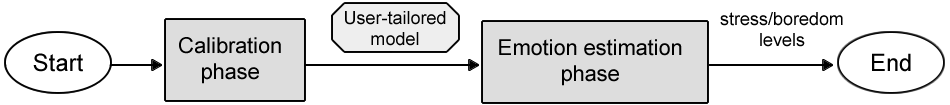
\includegraphics[width=\textwidth]{Content/figures/research-aim-general.png}
    \caption{General structure proposed for remote detection of stress and boredom levels of players during interaction with games.}
    \label{fig:research-aim-general}
\end{figure}

The process is based on a non-contact, multifactorial analysis of user signals obtained from a video stream via computer vision. The principal of the emotion detection phase is based on a user-tailored machine learning model, which is trained with information obtained from the user while he/she played a set of games in the calibration phase. The user-tailored machine learning model is trained according to the process presented in Figure \ref{fig:user-tailored-calibration}. Each user plays a set of calibration games while being recorded by a camera. Computer vision is used to process the video feed and remotely extract signals from the user, such as HR and facial actions. Those signals are used as input to train the machine learning model for that particular user (user-tailored model).

\begin{figure}[h]
    \centering
    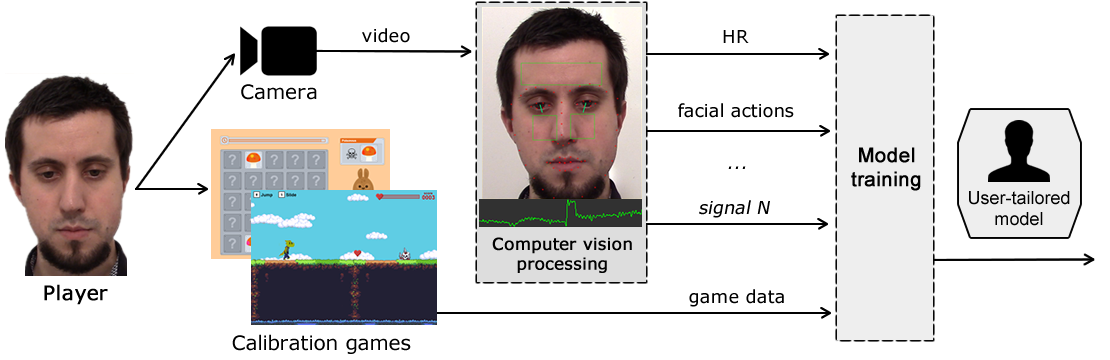
\includegraphics[width=\textwidth]{Content/figures/user-tailored-calibration.png}
    \caption{Calibration phase composed of emotion elicitation games (calibration games) and remote acquisition of signals from the user. The result of this phase is a user-tailored model used to detect emotions.}
    \label{fig:user-tailored-calibration}
\end{figure}

The games used in the calibration phase act as emotion elicitation sources. Each of those games are casual-themed and carefully designed to trigger two distinct emotions, i.e. boredom and stress, featuring a progressive transition between them as illustrated by Figure \ref{fig:calibration-game-linear}. At the beginning of the game, the difficulty level (green line) is low and the user is required to perform few or no actions. The games are designed in a way that the user is not able to increase the pace of the gameplay nor make it faster based on personal skills. As a consequence the user is forced to play a low-paced gameplay, which leads to an emotional state of boredom (blue curve). As time progresses, the pace of the gameplay and its difficulty level increase linearly. The increase happens at fixed time intervals, e.g. every 60 seconds. At some point in time, which is different for each user depending on gaming skills and personal preferences, the pace of the gameplay and the difficulty level will be overwhelming, leading the user to an emotional state of stress (red curve). As the difficulty level continues to increase, the stress level of the user will also increase. Finally the difficulty level will increase until the point where the user is unable to cope with the game, which will lead to consecutive mistakes in the game that will eventually terminate it, e.g. heath bar of the main character reaches zero.

\begin{figure}[h!]
    \centering
    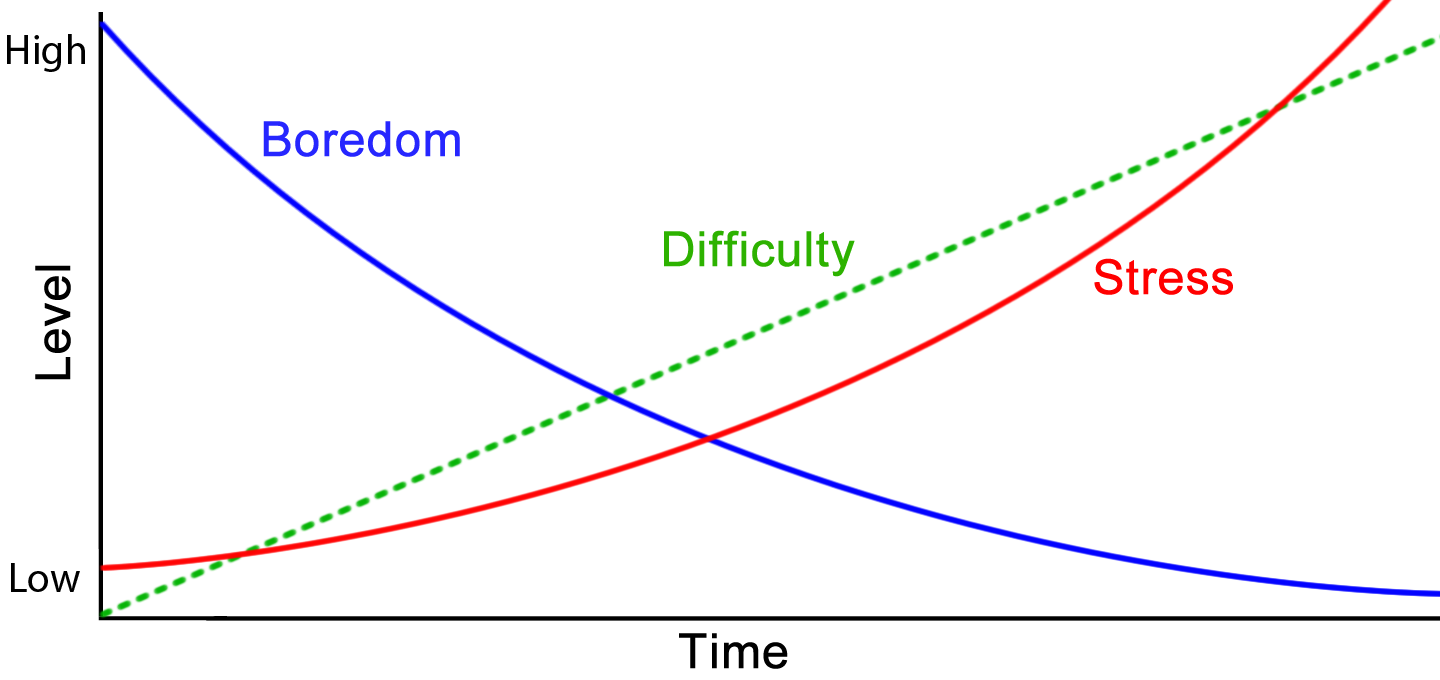
\includegraphics[width=0.7\textwidth]{Content/figures/calibration-game-linear.png}
    \caption{Progression of the level of difficulty of a calibration game over time along with the corresponding variations of the emotional states of stress and boredom experienced by the user.}
    \label{fig:calibration-game-linear}
\end{figure}

The mentioned calibration games are designed to trigger specific emotions and vary them over time, so the remotely collected information from the user during the calibration phase contains a detailed variation profile of the person being analyzed, including changes of each signal and the theoretically known emotional state of the user at that moment. If a person has a better response to a certain physiological signal instead of another, e.g. HR over facial expressions, then the variation of that signal accounts more weight in the training of the model. Since the training process is completely based on the signals of a single user, nuances and individual behavior are likely to be registered and learned. The calibration phase needs to be performed once per person.

After the calibration phase, the person can play any other ordinary game and be monitored in an emotion estimation phase, as illustrated by Figure \ref{fig:user-tailored-use}. As the user plays the game, signals are remotely acquired via computer vision. Those signals are used as input to the trained user-tailored model of that particular person, which produces as a result an estimation of the emotional state regarding stress and boredom for that person in that game. The process relies on the same remotely acquired signals with the addition of the predictions of the model according to the training performed during the calibration phase.

\begin{figure}[h]
    \centering
    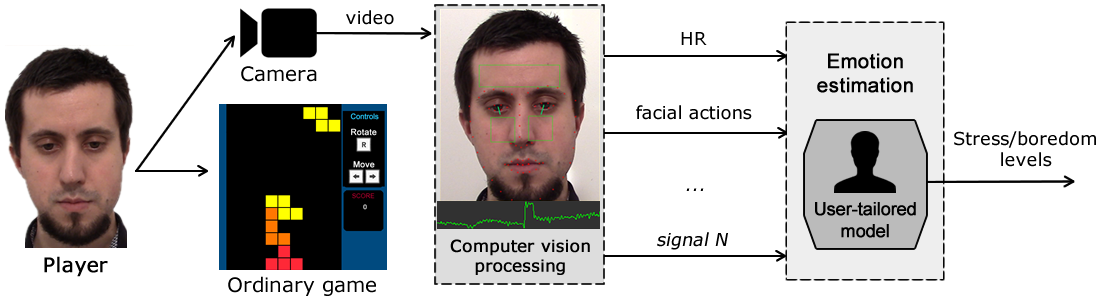
\includegraphics[width=\textwidth]{Content/figures/user-tailored-use.png}
    \caption{Emotion estimation phase. Remotely acquired signals from the user are fed into a user-tailored model that outputs the stress/boredom levels of the user during the interaction with an ordinary game.}
    \label{fig:user-tailored-use}
\end{figure}

Given that the user has a trained user-tailored model, the emotion estimation phase can be performed for any game as many times as desired. The model uses the remotely obtained signals from the user in conjunction with the calibration data to detect the player's changes regarding stress and boredom levels in any other game.

%According to previous research, the use of games as a emotional triggering mechanism is a feasible approach. Additionally an user-tailored model is a more efficient approach than a group-tailored model for the detection of emotional changes in users.
%\section{Thesis overview and structure}

\section{Thesis overview and structure}

This thesis is divided in parts whose chapters present and explain in details the scientific methodology, the theoretical background and the studies conducted to achieve the research aim described in Section \ref{sec:research-aim}. Overall the solution to remotely detect user emotions proposed by this thesis relies on three main elements: \textbf{emotion elicitation}, i.e. calibration games, \textbf{acquisition of users signals}, i.e. computer vision techniques, and \textbf{emotion estimation}, i.e. user-tailored machine learning model. Those three elements are significantly intertwined and they directly affect each other. In summary, when users interact with game-based emotion elicitation material, they tend to move, laugh and occlude the face, which adds noise to (or impede) the estimations performed by the computer vision techniques. It then affects or even prevents the creation of an emotion detection model, which requires the games to be re-worked or adapted to ensure they continue to serve as emotion elicitation material, consequentially leading to a chain reaction that cycles over the previously mentioned elements again.

According to the literature review conducted for this research, the use of those three main elements combined has never been tried before. As a result, it was not possible to determine beforehand if they could actually work in combination to detect user emotions remotely. A set of iterations would be required to test, evaluate and learn about those elements working together. On that account, Design Science, an iterative problem solving research method, was deemed the best approach to conduct the investigation, as explained in Chapter \ref{ch:methodology} (on page \pageref{ch:methodology}). Using such research method, the literature is consulted and a tentative solution is proposed and evaluated. Results of such evaluation provide new insights about the problem, which are then interpreted against the literature, leading to a new tentative solution. The cycle is repeated until a solid contribution is formed. For the research conducted in this thesis, the literature review made it clear that a more fruitful way of detecting emotions would be to interpret them as a manifestation of psychophysiological signals, e.g. HR and facial activity. It steers the research towards human physiology instead of psychology, whose interpretation is likely less subjective and more quantitative oriented. The literature review also focused on identifying which psychophysiological signals have been used in previous work focused on emotion detection, along with identification of computer vision techniques that can remotely extract those signals. After selecting the set of signals and computer vision techniques to be used in this research, six iteration of the design science cycle were performed based on two experiments. Experiment 1, detailed in Chapter \ref{ch:experiment1} (on page \pageref{ch:experiment1}), aimed to evaluate the feasibility of using the previously mentioned three main elements of this research in conjunction. It was mainly designed to test if the concept of calibration games, a novel aspect of the this thesis, would cause an emotional reaction on the subjects that could be remotely detected out of psycophysiological signals. Data gathered in experiment 1 was analyzed in five studies, i.e. Study 1 to 5, which can be seen as five iterations in the design science cycle.

\textbf{Study 1:} detailed in Section \ref{sec:experiment1-study1} (on page \pageref{sec:experiment1-study1}) was an exploratory evaluation of facial activity and perceived boredom and stress levels. The evaluation is connected to previous works and emotion/game theories presented in Chapters \ref{ch:literature-games} and \ref{ch:literature-face} (on pages \pageref{ch:literature-games} and \pageref{ch:literature-face}, respectively). Analysis of subject's self-reported emotional states statistically confirmed that they perceived the games as being boring at the beginning and stressful at the end. It supported the idea that calibration games, a corner stone in this thesis, could be used as emotion elicitation material. Additionally manual and empirical analysis of the video recordings indicated that subjects presented more facial actions during stressful periods of the games compared to boring periods. Finally there was indications that subjects featured a neutral face most of the time, which implies that it is not trivial to estimate emotions purely based on facial analysis without a context.

\textbf{Study 2:} detailed in Section \ref{sec:experiment1-study2} (on page \pageref{sec:experiment1-study2}) evaluated if calibration games could produce variations in physiological signals, namely HR, as described by the theories and previous work presented in Chapter \ref{ch:literature-physiological} (on page \pageref{ch:literature-physiological}). Analysis of the HR collected with a physical sensor, i.e. watch, during the experiment statistically confirmed that subject's HR was different during stressful and boring periods of the game. This information confirmed that calibration games could be used as emotion elicitation material, effectively inducing variations in physiological signals on subjects exposed to them, which could be used to detect emotions.

\textbf{Study 3:} detailed in Section \ref{sec:experiment1-study3} (on page \pageref{sec:experiment1-study3}) evaluated the feasibility of remotely detecting the variations of HR that were confirmed in Study 2. Remote photoplethysmography (rPPG), as described by the theories and works presented in Chapter \ref{ch:literature-rppg} (on page \pageref{ch:literature-rppg}), was used as the technique to remotely estimate HR information from videos of subjects interacting with games. Estimations of HR obtained with rPPG were compared to HR measurements collected with the physical sensor, which highlighted how the technique is affected by the natural behavior of subjects, e.g. movement and laughter. The study also provided insights about the mean estimation error of the technique when affected by the noise introduced by the natural behavior of subjects.

\textbf{Study 4:} detailed in Section \ref{sec:experiment1-study4} (on page \pageref{sec:experiment1-study4}) evaluated facial activity of subjects similarly to Study 1, however using a completely automated process relying on computer vision. A method to automatically track facial muscles connected to emotional reactions, which were reported by previous works detailed in Chapter \ref{ch:literature-face} (on page \pageref{ch:literature-face}), was developed and evaluated in the study. Results of the automated facial analysis conducted on all subjects statistically confirmed the findings of the manual analysis performed in Study 1, suggesting that subjects presented more facial activity during stressful than boring periods of the games.

\textbf{Study 5:} detailed in Section \ref{sec:experiment1-study5} (on page \pageref{sec:experiment1-study5}) was the first iteration in the design science cycle where all the three previously mentioned main elements of this research were in place and working together to detect the emotional state of subjects. Based on previous works presented in Chapter \ref{ch:literature-multifactorial} (on page \pageref{ch:literature-multifactorial}), a neural network was trained and used to remotely detect emotions. For each subject, two calibration games were used to train the model, i.e. user-tailored neural network, while one calibration game was left out to be used to evaluate the accuracy of remotely estimating the emotional state of the subject. Permutations were used to ensure all calibration games were used in the 2-training-1-testing configuration. Additionally different sets of signals, i.e. facial activity and HR, only facial activity, only HR, an so on, were evaluated in relation to the accuracy of emotion detection. The test was motivated by findings described in Chapter \ref{ch:literature-multifactorial} (on page \pageref{ch:literature-multifactorial}), which suggest that a multifactorial analysis, when more than one signal is used in the emotion detection process, yields better results than using a single signal in isolation. Results regarding the accuracy of the emotion estimation indicated that a multifactorial approach is indeed better suited for the process. Additionally results indicate that the proposed method is able to perform emotion estimations better than chance-level classification, which confirmed the feasibility of method proposed in this thesis. Finally the achieved results indicated that the jointly use of calibration games and remote acquisition of signals to train a user-tailored machine learning model can detect emotional states of users.

Following the confirmation of feasibility provided by Study 5, a new experiment was designed and conducted to validate the proposed method. At this point in the research project, the evaluation was conducted in larger scale compared to the first experiment and all the main elements of the proposed method were in place and working together. Experiment 2, detailed in Chapter \ref{ch:experiment2} (on page \pageref{ch:experiment2}), aimed to evaluate the accuracy of the final method proposed in this thesis to remotely detect emotions of users interacting with a game. In experiment 2, subjects played the same calibration games of experiment 1, however they also played 7 levels of Infinite Mario, detailed in Section \ref{sec:experiment2-evaluation-game} (on page \pageref{sec:experiment2-evaluation-game}), which is a clone of the commercial of-the-shelf (COTS) game Super Mario. Data from the calibration games was used to train a user-tailored neural network, which was used to estimate the emotional state of each subject during the interaction with the levels of Infinite Mario. Results confirmed in a larger scale the findings of the previously conducted Study 5, supporting the idea that the method proposed in this thesis for remote estimation of emotions is feasible.

\subsection{Text organization}

This thesis is structured to first introduce the methodology used to conduct the research, as presented by Chapter \ref{ch:methodology} (on page \pageref{ch:methodology}). Subsequently a literature review presents the theoretical background that support this research. Concepts, theories and techniques are presented and contextualized within the aims of this thesis, including emotions and games (Chapter \ref{ch:literature-games}, on page \pageref{ch:literature-games}), emotions and facial analysis (Chapter \ref{ch:literature-face}, on page \pageref{ch:literature-face}), emotions and physiological signals (Chapter \ref{ch:literature-physiological}, on page \pageref{ch:literature-physiological}), remote extraction of physiological signals (Chapter \ref{ch:literature-rppg}, on page \pageref{ch:literature-rppg}), and multifactorial emotion estimation (Chapter \ref{ch:literature-multifactorial}, on page \pageref{ch:literature-multifactorial}). Following is a part containing chapters related to the two experiments conducted to investigate, evaluate and validate the elements proposed by this research. Experiment 1 (Chapter \ref{ch:experiment1}, on page \pageref{ch:experiment1}) and its five studies show how the method proposed in this thesis was constructed. Experiment 2 (Chapter \ref{ch:experiment2}, on page \pageref{ch:experiment2}) shows how the proposed method was evaluated in larger scale in a scenario that is more similar to a real use case. Afterwards is the part of the thesis that presents the results achieved by this research project, along with a discussion of its implications in the field of games research and other areas (Chapter \ref{ch:discussion}, on page \pageref{ch:discussion}). This part also includes chapters that discuss ethical and privacy considerations of this research (Chapter \ref{ch:ethics}, on page \pageref{ch:ethics}), as well as limitations and critiques related to the proposed method (Chapter \ref{ch:limitations}, on page \pageref{ch:limitations}). Finally the last part presents the closing remarks with a conclusion (Chapter \ref{ch:conclusion}, on page \pageref{ch:conclusion}) and suggestions of future work (Chapter \ref{ch:closing}, on page \pageref{ch:closing}).

\subsection{Definitions and scope}

The research presented in this thesis is a multidisciplinary work that involves theories and concepts from different fields. Some of those concepts, particularly regarding emotions, are shared among the fields, however they have different definitions and interpretations. As a consequence, it is important to establish what are the fields involved in this research, as well as the understanding of concepts in the context of this work, particularly regarding emotions. Figure \ref{fig:fields} illustrates the fields related to this research alongside with the community that the work contributes to.

\begin{figure}[h]
    \centering
    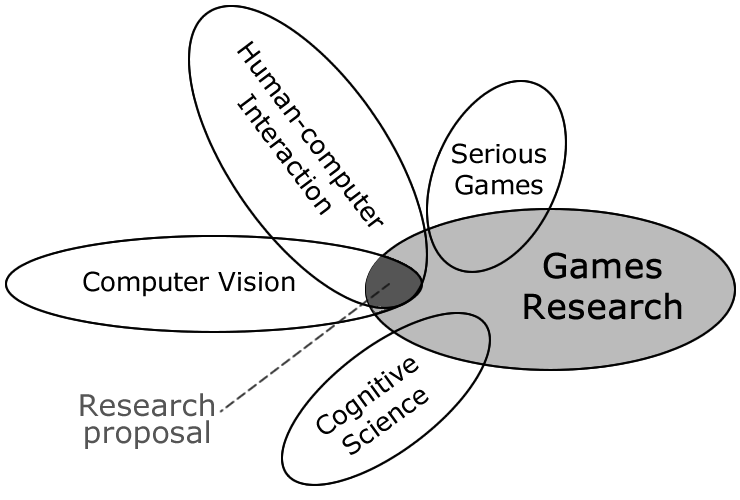
\includegraphics[scale=0.6]{Content/figures/fields}
    \caption{Different fields involved in this research. Main contribution is on the area of Games Research.}
    \label{fig:fields}
\end{figure}

The present research mainly involves and contributes to the field of games research, particularly the branch related to variations of emotions during interactions of users and games. The process of monitoring user emotions in human-computer interaction, known as affective computing \parencite{picard2000affective}, is a challenging endeavor and a recurrent research topic. This thesis brings concepts of Computer Vision into the field of Games Research to enhance the process of monitoring user emotions, making it non-obtrusive by proposing a method to remotely acquire and analyze player's signals in order to detect stress and boredom levels. Despite being connected to the topic of human emotions, this research does not focus on Cognitive Science, whose definition of stress and boredom, for instance, might carry a different meaning and correlation with games. Stress and boredom, in the context of this research, are emotions used in the games research field to describe the state of mind of players during the interaction with games. Stress, in the scope of this research, is a state of mind self-reported by a player during a game session that expresses a high level of anxiety, particularly when the player's skill level is not sufficient to beat the current challenge in the game. Similarly, boredom is a state of mind self-reported by a player during a game session that expresses a low level of enjoyment, particularly when the player's skill level is higher than the required to beat the current challenge in the game. Chapter \ref{ch:literature-games} (on page \pageref{ch:literature-games}) presents different theories related to emotions that can be used to define stress and boredom in games. In the context of this research, the definition of emotions, i.e. stress and boredom, is less related to Psychology or Cognitive Science. Instead the definition is based on Biology with focus on the human physiology, i.e. emotions are variations of psychophysiological signals, as seen in the ``fight or flight" effect. It is out of the scope of this thesis to create a (new) definition of stress and boredom based on the analysis of psychophysiological signals. On the contrary, the analysis of such signals and their variations are the source of information used to classify the emotional state of subjects.

\chapter{Research methodology}

The aim of this research is to produce a technology-based solution to the problem of non-contact emotion detection within the context of games research. The solution is a software composed of a user-tailored model that is trained from a game-based calibration phase and is able to infer the emotional state of a player regarding stress and boredom via analysis of remotely acquired user signals. The constructs, models and methods involved in such aim have been individually studied in previous research, however the combination of all those elements in a single solution within the context of games research is novel. The utilization of those elements in combination is not yet demonstrated to work, so an iterative and incremental process must be conducted to identify challenges, problems and solutions to achieve the desired goal.

\begin{figure}[h]
    \centering
    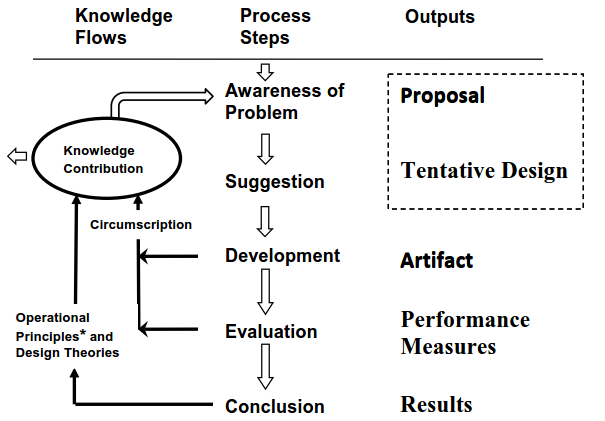
\includegraphics[width=0.8\textwidth]{Content/figures/vaishnavi-design-science-process-model.png}
    \caption{Design science research process model. Reproduced from \textcite{vaishnavi2004design}.}
    \label{fig:vaishnavi-design-science-process-model}
\end{figure}

A research methodology that fits such iterative process is design science. Typically design science research is a problem solving process focused on developing new artifacts. \textcite{hevner2004design} defines design science in the context of Information Systems as a process that explores a relevant problem within an environment, iteratively measuring and refining the proposed solution according to the existing body of knowledge. The progress is made iteratively as the scope of the design of the artifact is expanded based on the discovery of available means, ends and constraints. Similarly \textcite{johannesson2014introduction} define design science as the scientific study and creation of artifacts as they are developed and used by people with the goal of solving practical problems of general interest. The outcome of design science research includes the contextual knowledge about the artifacts.

\textcite{vaishnavi2004design} structure the mentioned iterative process in five steps, illustrated in Figure \ref{fig:vaishnavi-design-science-process-model}: awareness, suggestion, development, evaluation and conclusion. The awareness step is the recognition and articulation of a problem from an environment, which can be originated from studying the existing literature, for instance. The suggestion step presents a tentative design of how the problem might be addressed, which envisions a new functional artifact with a novel configuration of existing and/or new elements. The development and the evaluation steps comprehend the implementation of the tentative design and its analysis with well defined metrics and measurements. The evaluation either confirms or contradics hypothesis about the behavior of the object, leading to new awareness (and other iteration of the process) or to a conclusion. Finally the conclusion step determines why and how the artifact worked or did not work within its environment. \textcite{vaishnavi2004design} categorize the knowledge that is gained during the research process and presented in the conclusion step as \textit{firm} and as \textit{loose ends}. In the former the conclusion show facts that can be repeatably applied or behavior that can be repatably invoked, while in the later the conclusion shows anomalous behavior that defies explanation and may serve as further research topics.

The types of artifacts resulting from design science research are constructs, models, methods and/or instantiations \parencite{oates2005researching,johannesson2014introduction}. Contructs are the terms, concepts, definitions and notations required to formulate and represent the problem. Models are a combination of contructs related to each other to represent possible solutions to a problem. Methods provide guidance on the models to be produced and the process to solve the problem. Finally instantiation is a working system that demonstrates that theories and artifacts, i.e constructs, models and methods, can be implemented in a computer-based system.

\begin{figure}[h]
    \centering
    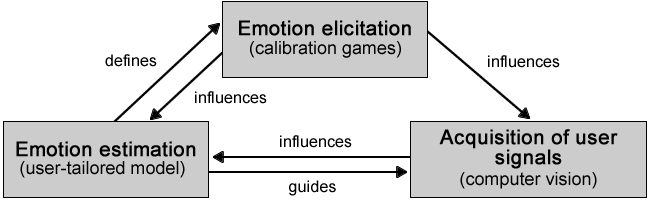
\includegraphics[width=0.8\textwidth]{Content/figures/method-components-dependency.png}
    \caption{Depency among the main parts of this research: emotion elicitation, acquisition of user signals and emotion estimation.}
    \label{fig:method-components-dependency}
\end{figure}

The present research involves the use and orchestration of three main components, illustrated in Figure \ref{fig:method-components-dependency}. Those components are a game-based emotion elicitation part, composed of calibration games, the part involving remote acquisition of user signals via computer vision, and an emotion estimation part, composed of a machine learning model. The use of game-based material in a calibration phase in this research influences how users behave during the emotion elitication process, e.g. body movement and facial expression. The movement of users directly impacts the techniques for remote extraction of user signals during both the calibration phase and the emotion estimation phase, since those techniques are highly influenced by motion. The accuracy of those techniques regarding the remotely acquired signals is affected as well, which might invalidate the feasibility of remotely reading determined physiological and non-physiological signals required by the emotion estimaion model.

The interaction among the mentioned components, i.e. emotion elicitation, acquision of user signals and emotion estimation, must be continuously investigated and adapted to overcome the previously described challenges. As a consequence, an iteractive cycle of development and research is required, as illustrated by Figure \ref{fig:hevner-generate-test}. In each iteration, a possible solution for the current set of problems is generated, rigourly tested and evaluated, producing information to guide the next iterations in the cycle. The set of design alternatives in this research are related to the identification of physiological and non-physiological signals to be used in the emotion estimation process, how they can be elicitated with games in a calibration phase, which computer vision techniques can be employed to remotely acquire the signals and which machine learning model is able to map the information into emotional states. The set of constraints involve problems associated with users behaving naturally, e.g. laughing and moving the body during the procedure, use of non-specialized hardware, e.g. ordinary camera, accuracy and efficienty of the solution, among others.

\begin{figure}[h]
    \centering
    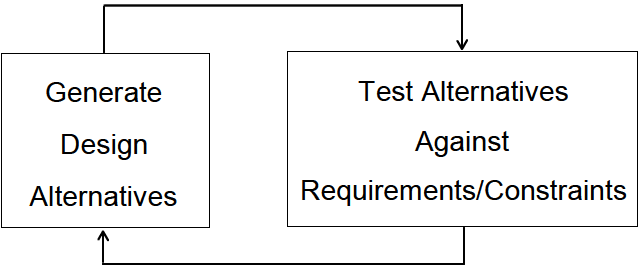
\includegraphics[width=0.6\textwidth]{Content/figures/hevner-generate-test.png}
    \caption{The Generate/Test cycle. Adapted from \textcite{hevner2004design}}
    \label{fig:hevner-generate-test}
\end{figure}

%The aim of this research is to produce a utility tool, i.e. software, which is an artifact based on a model built on existing theories, which will be combined in a new and innovative way. Since the result of the research is a model, which will be built from different measurements to predict or infer a state, the present work stands on the positivism paradigm. Essentially this work will formulate a theory about how the variation of physiological signals relate to stress/boredom levels in the context of games and how it can be remotely detected. The involvement of humans in the process might relate to the social side of interpretivism, however the foundation of the work is still based on the analysis of physiological signals. Such signals and their patterns might be different for each person, however they are still ordered and regular under the human being perspective. As a consequence, they can be objectively observed, measured and analysed with a quantitative approach and hypothesis testing.

Design-science research requires the application of rigorous methods in both the construction and evaluation of the designed artifacts \parencite{hevner2004design, johannesson2014introduction, oates2005researching}. One of such evaluation methods is experimental research, which is the strategy used to build and validate the knowledge in this project. Such approach is composed of a set of research designs that use controlled testing and manipulation of variables in order to understand causal processes \parencite{robson2016real}. The foundation of an experiment is to manipulate a variable (or a set of them) and measure any changes in other variables. It establishes the effect on a dependent variable, which is the focus of the research. The model being constructed in this research links the variations of user signals to stress/boredom levels in the context of games, hence there is a causal effect in the process since identified variations (cause) will precede changes in stress/boredom levels (effect). It progresses to the construction of a hypothesis where the cause will consistently lead to the same effect so the link between variations of signals and emotional levels can be inferred or predicted.

The preferred experimental design for the present research will be based on a within-subject approach \parencite{lane2015online}. In such approach, all participants perform at all levels of the treatment and there are no control groups.
%It is the opposite of a between-subjects approach, where subjects are divided in more than one group that receive different treatments. In that approach there are special groups, called control groups, that receive no treatment. The comparison between the control groups and the treatment groups ensures internal validity.
Such design could be criticized for having low internal validity, since it is not possible to unambiguously attribute cause and effect \parencite{kirk1982experimental}. A two-group approach could be suggested as having stronger internal validity, since it contains a control group and allows a less ambiguous conclusion. In the context of the present research, however, any multiple group design implies the comparison of physiological signals and emotional perceptions among different people. Given the social and cultural background of the participants, it is virtually impossible to compare two groups of people regarding stress/boredom. People have different preferences, culture and expectations, which cause maturation and history threats to internal validity \parencite{trochim2001research}.
%Additionally the process of comparing variations of physiological signals among different subjects is a complex task, even when subjects are similar, e.g. same age and sex. As a consequence, a subject in a control group might present a set of variations of signals and classify a game as boring, while a similar subject in another group might classify the same game as not boring at all, presenting a different set of variations of signals.
In that light, the within-subject approach relies on a one-group experimental design to increase internal validity, since subjects are compared with themselves, which removes inter-subject differences.

Design science research is a feasible approach for this research project. The iterative nature of the methodology allows the investigation, validation and better understanding of the interactions among the component involved in the proposed research aim. The research is expected to produce a main artifact, i.e. emotion detection process, however it will be composed of several other artifacts including models, methods and the instantiation of the complete solution.

%\section{Research objectives}

%The objective of this research is to produce a method that is able to interpret remotely acquired signals from a person playing a game and detect his/her current emotional state regarding stress and boredom according to data previously obtained in a calibration phase. The model will be implemented in a software that uses a video feed to detect the person's emotional state.

%The current approaches used to obtain information from the players during games research inevitably affect the player's experience. They require the user to stop the game activity in order to share his/her current state, such as by answering a questionnaire. The frequency that such questionnaires are issued is also a concern. If performed too often, more information might be collected, but the data might contain noise caused by the frequent interruptions, e.g. player is more stressed/bored by the questionnaire interruptions than by the game itself. If performed too sparse, not enough information will be gathered from the player. A physical sensor attached to a player, on the contrary, allows a continuous monitoring process, however it is intrusive and might interfere with the player capacity to interact with the game. It might prevent the use or movement of specific parts of the body, for instance. Physical sensors also increase the chances of the player to behave differently as a side-effect of the monitoring process itself.

%A purely remote-based solution, as the one proposed by this research, enhances the tooling available to the games research community regarding investigation methods of stress and boredom. A games researcher will be able to increase the internal validity of his/her workflow by ensuring the player keeps the focus on the game without interruptions and by minimizing the side effects (and inconveniences) of physical monitoring. This research could also be deployed as a solution for game developer studios to automatically analyze hours of recorded gameplay and highlight the moments when boredom/stress levels changed significantly. As a complement the solution will be based on a single, ordinary camera and a software implementation, which eliminates the use of complex setups of physical sensors. It eases the investigation process and reduces costs.

\part{Literature review}
\chapter{Games and emotions}
\label{ch:literature-games}

Research about games is a broad topic that involves different disciplines and definitions. In the context of this thesis, a game is defined as a system in which players engage in an artificial conflict, defined by rules, that results in a goal \parencite{salen2004rules}. An artificial conflict is a set of challenges that the player must overcome towards the game goal, e.g. sort elements within a time constraint.

\textcite{schell2014art} mentions that, from a game design perspective, the difficulty level of such challenges affects the emotional state of players, e.g. moments of boredom or anxiety/stress. Every time a reward is given to the player, which usually is a tool to increase the player's power, the game's challenge level is lowered because the player becomes more skilled. After a period, such increase in the player's skill level causes the game to be boring because the challenges are now easier to beat. At that point, the difficulty level is again increased by the game, raising the challenging levels for the player once more, causing anxiety. The anxiety and stress period lasts until the player is rewarded again, when the newly obtained power will eventually lower the challenge levels again (resulting in boredom), causing the cycle to repeat itself.

\textcite{chen2007flow} used the theory of flow or the ``theory of optimal experience'', originally estaslished by \textcite{csikszentmihalyi1991flow}, to describe how player experience was in large part depending on the relationship between a game's challenge and its player's level of skill. A challenge beyond the player's skill to address and overcome it causes anxiety, while the opposite results in disinterest, leading to boredom \parencite{chen2007flow}. An ideal challenge/skill balance in a repeating cycle of increasing challenge followed by a reward keeps the player in an optimal experience and concentration, i.e. flow zone, as illustrated by Figure \ref{fig:flow-schell}.

\begin{figure}[h!]
    \centering
    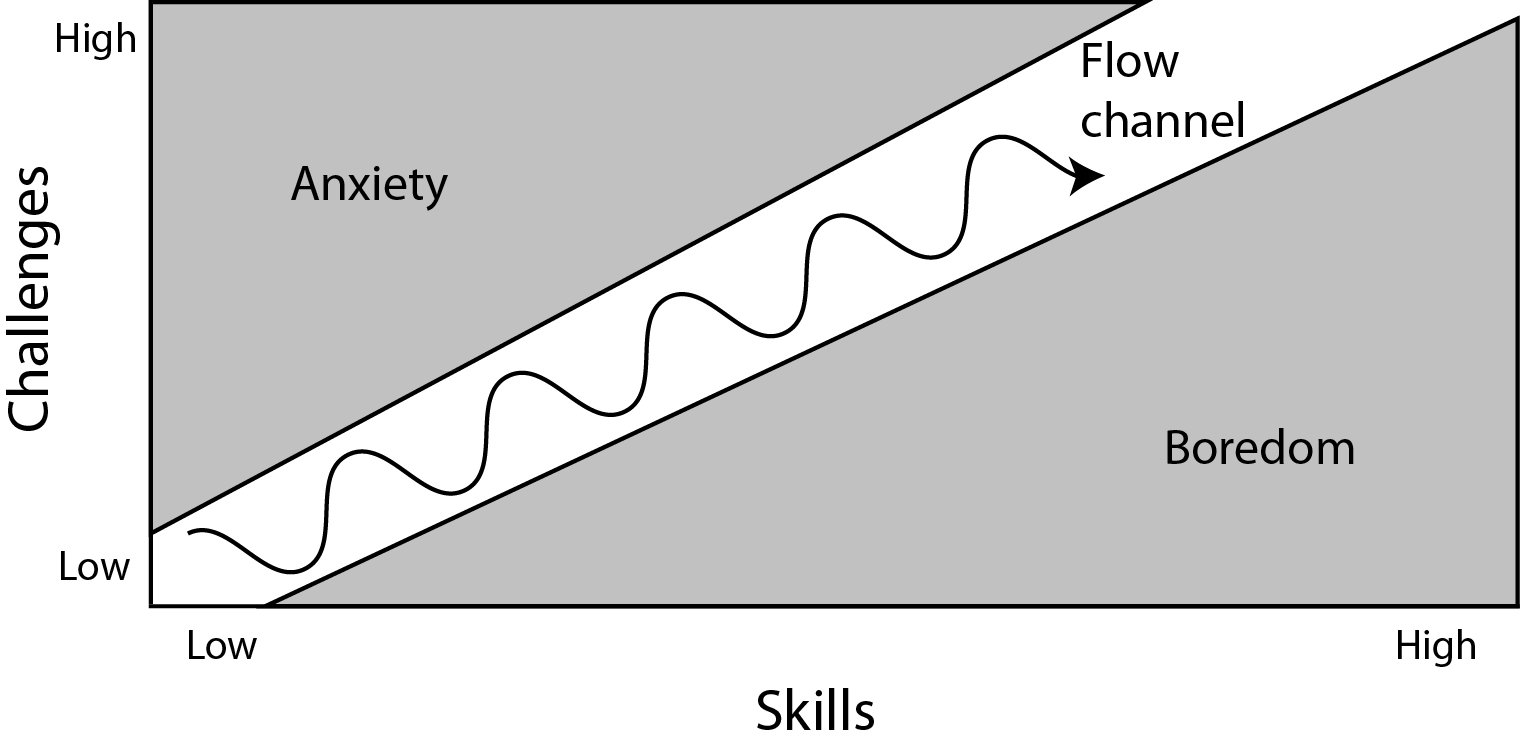
\includegraphics[scale=0.8]{Content/figures/flow-schell.png}
    \caption{Repeating cycle of increasing challenge followed by a reward, keeping the player in the flow zone. \parencite{schell2014art}}
    \label{fig:flow-schell}
\end{figure}

 The following sections describe in more detail the theoretical foundation of emotions, connecting them to the context of games.

%%%%%%%%%%%%%%%%%%%%%%%%%%%%%%%%%%%%%%%%%%%%%%%%%%%%%%%%%%%%%%%%%%%%%%%%%%%%%%%%%%%%%%%%%%%%%%%%%%%%%%%
\section{Emotions theory}
%%%%%%%%%%%%%%%%%%%%%%%%%%%%%%%%%%%%%%%%%%%%%%%%%%%%%%%%%%%%%%%%%%%%%%%%%%%%%%%%%%%%%%%%%%%%%%%%%%%%%%%

In the field of games research, one of the most mentioned theories regarding emotions is the theory of flow. It has been used as the foundation for several concepts, including engagement and immersion \parencite{brown2004grounded}, sense of presence \parencite{weibel2011immersion} and applicability in game design \parencite{sweetser2005gameflow, chen2007flow, cruz2017player}. Flow was originally defined as a phenonmenon in which a person experiences a subjective state characterized by an instense level of attention during the execution of an intrinsically motivated activity \parencite{csikszentmihalyi1991flow}. As previously mentioned, an ideal challenge/skill balance in a game leads players to an optimal experience and concentration state (e.g. flow), so flow constructs are of interest to the games community. Such peculiar state of flow, however, is not limited to activities involving games, it can be experienced in a variety of other activities, e.g. dancing and climbing. The connection of the theory of flow to contexts other than games is outside the scope of this thesis.

Further research \parencite{nakamura2014concept} refined the original definition of the flow state, culminating in the eight channel model of flow, illustrated in Figure \ref{fig:flow-eight}. Such model better describes the emotional state of users according to the challenge/skill balance in relation to the subject mean, since it is less coarse than the original flow model. In the eight channel model of flow, for instance, a person performing a low skill and low challenging task experiences apathy, while in the original model the classification would indicate a flow state. Emotional states as stress and boredom can be described as a function of the current player's skill level and the level of challenge he/she is facing.

\begin{figure}[h!]
    \centering
    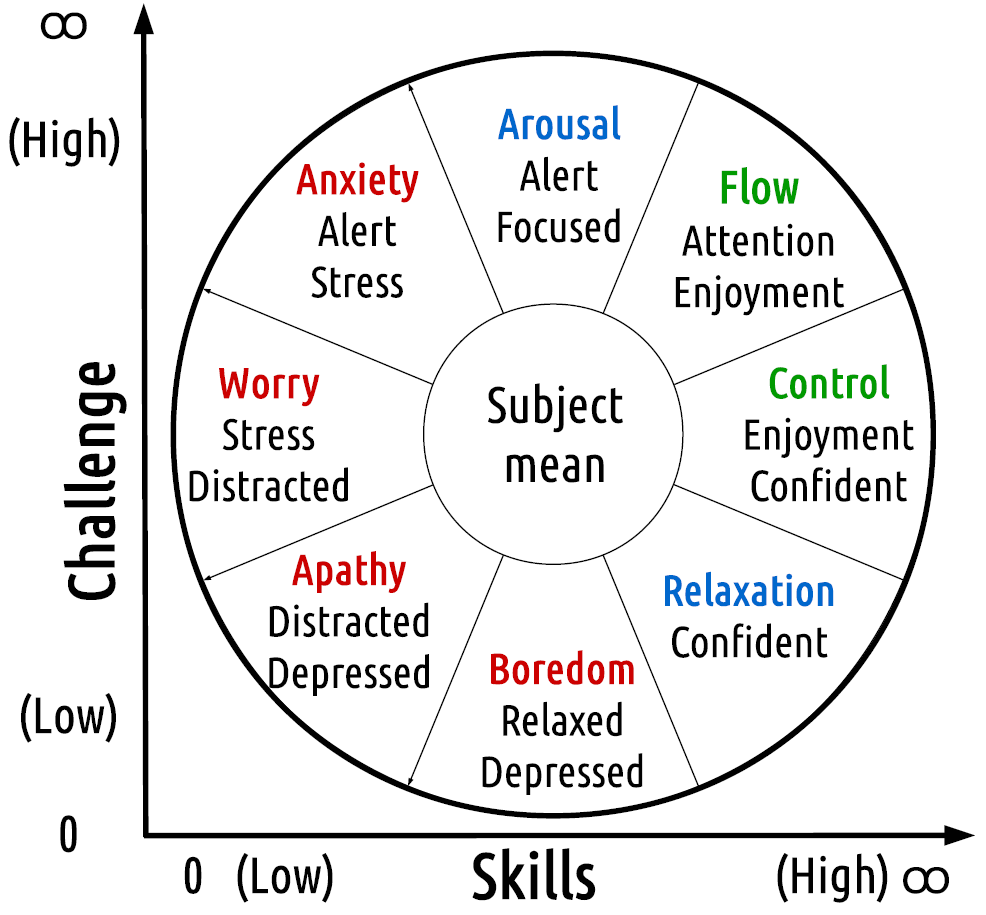
\includegraphics[scale=0.3]{Content/figures/flow-eight.png}
    \caption{Eight channel model of flow \parencite{nakamura2014concept}}
    \label{fig:flow-eight}
\end{figure}

Another model commonly mentioned in the literature are the basic emotions proposed by \textcite{ekman1971constants}. Constructed from an experiment involving cultural differencies, it states that particular facial muscular patterns and discrete emotions are universal. The six emotions mentioned in the theory are happiness, surprise, sadness, fear, anger and disgust, which are strictly basic emotion models of affective state. A contrary definition is presented by \textcite{russell1978evidence}, who defined another model of emotions named Circumplex Model of Affect (CMA). Commonly referred to as Russell's Arousal-Valence (AV) space, the model is contrary to strictly basic emotion models of affective state, where each emotion emerge from independent neural systems \parencite{posner2005circumplex}. The model proposes a dimensional approach where all affective states arise from the activation of two fundamental neurophysiological systems: arousal (or alertness) and valence (a pleasure–displeasure continuum).

\begin{figure}[h!]
    \centering
    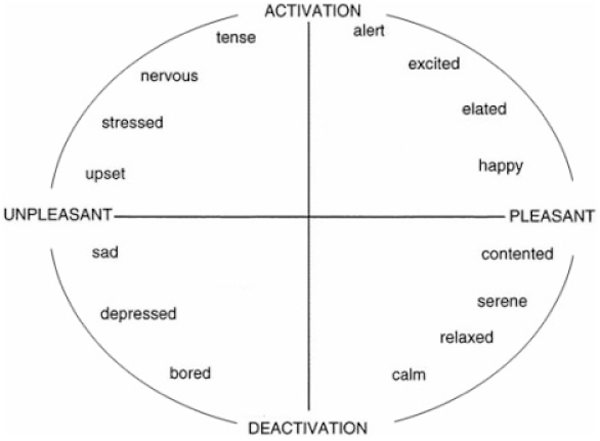
\includegraphics[scale=0.5]{Content/figures/russell-av.png}
    \caption{Representation of the circumplex model of affect \parencite{posner2005circumplex}. Horizontal axis represents the valence dimension and the vertical axis represents the arousal or activation dimension.}
    \label{fig:av-model}
\end{figure}

Figure \ref{fig:av-model} illustrates the AV space. The horizontal axis represents the valence dimension, which varies from the negative, unpleasant spectrum to the positive, pleasant spectrum. The vertical axis represents the arousal or activation dimension, which varies from low (bottom) to high (top). Each emotion is the result of a linear combination of these two dimentions. An emotional state of excitement, for instance, is conceptualized as the product of a positive activation in the neural system associated with valence along with a high activation in the neural system associated with arousal. The different scales of activation of each of those two dimensions produces different emotional states.

%%%%%%%%%%%%%%%%%%%%%%%%%%%%%%%%%%%%%%%%%%%%%%%%%%%%%%%%%%%%%%%%%%%%%%%%%%%%%%%%%%%%%%%%%%%%%%%%%%%%%%%
\section{Immersion, engagement and sense of presence}
%%%%%%%%%%%%%%%%%%%%%%%%%%%%%%%%%%%%%%%%%%%%%%%%%%%%%%%%%%%%%%%%%%%%%%%%%%%%%%%%%%%%%%%%%%%%%%%%%%%%%%%

As previously mentioned, the theory of flow is significantly used to explain emotional states and concepts in the field of games research. The definition of flow, however, requires a more sophisticated interpretation, as investigated by further research. %As previously mentioned, from a game design perspective, for instance, Schell \parencite{schell2014art} mentions that a progression of the player in the flow zone is desired, however it should not be a ``straight line'', but more of a cycle alternating among emotional states as stress, enjoyment and boredom.
Different elements are also connected to flow, such as engagement, immersion and sense of presence.

Immersion, in the concept defined by \textcite{brown2004grounded}, refers to the degree of involvement of players with a computer game. In that light, the authors theorize that a player overcomes barriers that limit his/her degree of involvement in immersion. After each barrier is broken, the sense of immersion deepens. The first barrier, for instance, is named engagement and it refers to the player willingness to invest attention and energy to learn how to play the game. The concept of flow, as defined by \textcite{csikszentmihalyi1991flow}, is an extreme state, which is only achieved when the player has overcame all previously mentioned barriers and is in a ``total immersion'' state. Such condition is rare to happen since it requires the highest level of attention from the player. As a consequence, engagement is more plausible and common during gaming experiences than flow.

The existence of several works \parencite{boyle2012engagement} related to understanding and defining what engagement and immersion are demonstrates the interest of researchers to broaden the view beyond flow alone. Presence, for instance, which describes the player's feeling of actually being in the game, is reported as an important aspect of engagement and immersion \parencite{weibel2011immersion}. Studies connected to training simulation \parencite{engstrom2016impact}, for instance, also indicate that contextualization (increasing the sense of presence) might affect immersion positively. Additionally to the intentions of understanding and defining engagement and immersion, studies also try to measure them. The majority of the approaches used for that are based on questionnaires, which are by nature subjectively answered by players. Additionally that approach usually breaks any sense of presence of the player since it requires a shift in attention away from the game, hence breaking or affecting the level of engagement/immersion as well.

Quantitative approaches have also been investigated to measure engagement, such as the use of physiological signals like heart rate \parencite{ravaja20051} and eye movement \parencite{jennett2008measuring}, for instance. The complexity in defining engagement and immersion is also reflected in the task of measuring it. \textcite{ravaja20051}, for instance, mentions the significant variation of physiological signals as an obstacle. Signals increase during emotional arousal, but decrease in response to attention engagement, which makes the measurement of engagement a non-trivial process. It highlights the difficulties in correlating qualitative data to more abstract concepts as engagement, immersion and flow.

%Research initiatives that help in the identification of the player emotional state without breaking the current level of engagement and immersion are desired. This research aims at using the link between the ANS and emotional regulation as the foundation to analyse physiological signals of a player, which will be remotely obtained and processed in a user-tailored fashion according to data previously collected in a game-based calibration phase.

%%%%%%%%%%%%%%%%%%%%%%%%%%%%%%%%%%%%%%%%%%%%%%%%%%%%%%%%%%%%%%%%%%%%%%%%%%%%%%%%%%%%%%%%%%%%%%%%%%%%%%%
\section{Instruments for assessment of emotions}
%%%%%%%%%%%%%%%%%%%%%%%%%%%%%%%%%%%%%%%%%%%%%%%%%%%%%%%%%%%%%%%%%%%%%%%%%%%%%%%%%%%%%%%%%%%%%%%%%%%%%%%

Questionnaires are a common tool used for the assessment of emotional states of users during experiments involving games and emotions. Different formats of questionnaires are found in the literature. The simplest approach are ad-hoc questionnaires, which contains a set of questions designed by the researcher for a particular experiment. A common type of emotion scale in such approach are Likert scales related to an emotional state, e.g. stress level.

Another instrument for assessment of emotions is the Self-Assessment Manikin (SAM) \parencite{morris1995observations}, which is an efficient cross-cultural measurement of emotional response regarding pleasure, arousal and dominance. Figure \ref{fig:sam} illustrates the SAM mechanism. SAM employes a nonverbal, graphic depiction of three affective dimensions. In the top row of the questionnaire the user can express the level of pleasure, ranging from a figure with a smile to a figure with an unhappy face. The middle row presents figures ranging from an agitated (high arousal) state to a relaxed, sleepy state. Finally the bottom row represents the level of dominance (control) of the user in the situation at hand.

\begin{figure}[h]
    \centering
    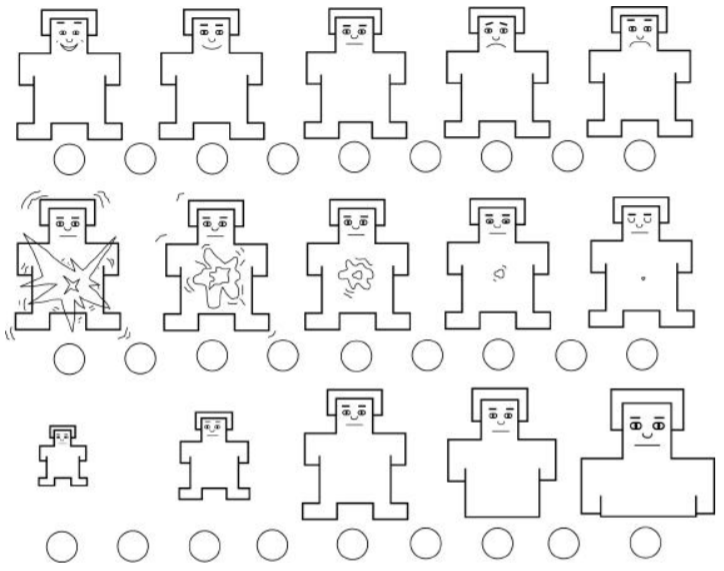
\includegraphics[width=0.7\textwidth]{Content/figures/SAM.png}
    \caption{Self-Assessment Manikin (SAM). Reproduced from \textcite{morris1995observations}.}
    \label{fig:sam}
\end{figure}

A similar approach is the Affective Slider (AS) \parencite{betella2016affective}, a digital self-reporting tool composed of two slider controls for assessment of pleasure and arousal. Figure \ref{fig:as} illustrates the AS self-assessment mechanisms. AS also employes a nonverbal, graphic depiction of the emotional state of the user, however the focus is on arousal and valence. A user can adjust the sliders to show his/her level of arousal (top slider) and valence (bottom slider).

\begin{figure}[h]
    \centering
    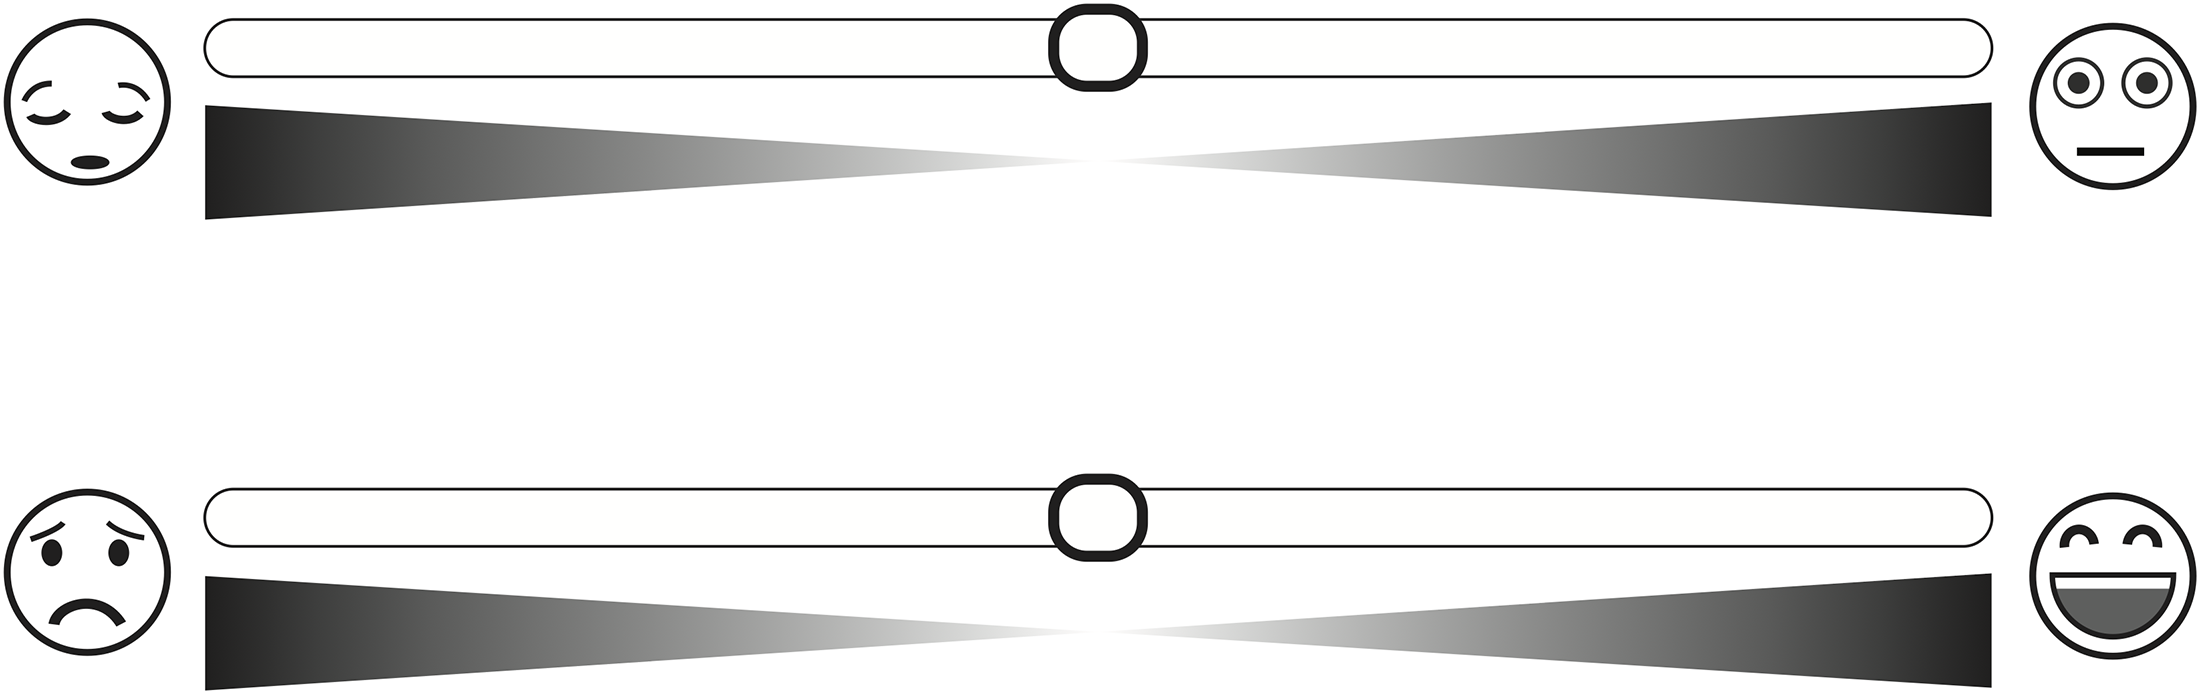
\includegraphics[width=0.7\textwidth]{Content/figures/AS.png}
    \caption{Affective Slider (AS). Reproduced from \textcite{betella2016affective}.}
    \label{fig:as}
\end{figure}

The selection of an emotion assessment instrument is connected to the research context. Both SAM and AS, for instance, are established and proven emotion measurement instruments, which would strengthen the theoretical foundations of the emotion measurement process. As a downside, however, they require the researcher to instruct users on how to properly answer the questionaire.

\chapter{Emotions and facial analysis}
\label{ch:literature-face}

The human face is a source of information and an important part of communication. Several elements connect this channel of information to emotional states, such as facial expressions and the activity of eyes and head \parencite{akakin2010spatiotemporal}. The analysis of such elements can convey information regarding emotional states, e.g. facial expressions are considered one of the most relevant features that can provide indication about emotional states \parencite{cowie2001emotion}.

Facial analysis is a promising approach to detect the emotional state of players unobtrusively and without interruptions \parencite{cohn2014automated}. The use of computer vision for player experience detection is feasible and visual inspection of gaming sessions has shown that automated analysis of facial expressions is sufficient to infer the emotional state of players \parencite{tan2012feasibility,tan2014inferring}. Automatically detected facial expressions have been correlated with dimensions of game experience \parencite{tan2014correlation} and used to enhance player's experience in online games \parencite{zhou2004real,zhan2008real}. Automated facial analysis has become mature enough for affective computing, however there are several challenges associated with the process. Facial actions are inherently subtle, making them difficult to model, and individual differences in face shape and appearance undermine generalization across subjects \parencite{cohn2014automated}. Schemes such as the Facial Action Coding System (FACS) \parencite{ekman1977facial,cohn2007observer} aim to overcome those challenges by standardizing the measurements of facial expression by defining highly regulated procedural techniques to detect facial Action Units (AU). In the FACS scheme, facial actions/movements are decomposed into 46 different AUs anatomically related to facial muscles. When analyzed in defined contexts, such mapped actions can present a correlation between determined facial features and emotional states, e.g. stress and boredom.

\begin{table}[h!]
\caption{Categorization of facial elements connected with stress and anxiety according to \textcite{giannakakis2017stress}}
\label{table:stress-facial-features}
\begin{tabular}{lll}%
\toprule%
\textbf{Head} & \textbf{Eyes} & \textbf{Mouth} \\
\midrule
Head movement & Blink rate & Mouth shape \\
Skin color & Eyelid response & Lip deformation  \\
Heart rate (facial PPG) & Eye aperture & Lip corner puller \\
& Eyebrow movements & Lip corner depressor \\
& & Lip pressor \\
\midrule
\textbf{Gaze} & \textbf{Pupil} & \\
\midrule
Saccadic eye movements & Pupil size variation &  \\
Gaze spacial distribution & Pupil ratio variation &  \\
Gaze direction & &\\
\bottomrule%
\end{tabular}%
\end{table}

\textcite{giannakakis2017stress} present a literature review focused on facial elements with value for detection of anxiety and stress, including the involvement of eyes (pupil size variations, gaze distribution, blinking rate), mouth (lips deformation, mouth activity) and head (head movement and velocity). Table \ref{table:stress-facial-features} lists all identified facial elements. There are indications that blinking increases with emotional arousal, including stress and anxiety levels \parencite{dinges2005optical}. Gaze direction, gaze congruency (agreement between eye and head orientation) and the size of the gaze-cuing effect (facilitation of reaction time towards visual clues) are also influenced by the level of anxiety or stress \parencite{staab2014influence}. Similarly mouth activity is influenced by conditions of stress, particularly lip movement \parencite{dinges2005optical} and asymmetric lip deformation \parencite{metaxas2004image}. Finally the frequency of mouth openings has been measured as inversely proportional to the stress level under high cognitive load \parencite{liao2005decision}.

Different approaches have been used to connect facial analysis to emotional states of users. Initiatives include manual or automated face detection, use of machine learning models to map facial features to emotions and so on. The following sections present in more detail works related to face detection, including the approach used for analysis and connection to emotional states.

%%%%%%%%%%%%%%%%%%%%%%%%%%%%%%%%%%%%%%%%%%%%%%%%%%%%%%%%%%%%%%%%%%%%%%%%%%%%%%%%%%%%%%%%%%%%%%%%%%%%%%%
\section{Facial analysis based on sensors}
%%%%%%%%%%%%%%%%%%%%%%%%%%%%%%%%%%%%%%%%%%%%%%%%%%%%%%%%%%%%%%%%%%%%%%%%%%%%%%%%%%%%%%%%%%%%%%%%%%%%%%%

Analysis of facial behavior commonly relies on data obtained from physical sensors, e.g. electromyography (EMG), or from the application of visual methods to assess the face, e.g. feature extraction via computer vision \parencite{schrader2017rising}. The approach based on EMG data uses physical sensors attached to subjects to measure electrical activity of facial muscles, such as the zygomaticus, the orbicularis oculi and the corrugator supercilii muscles (Figure \ref{fig:face-muscles}), associated with smiling, eyelids control and frowning, respectively.

\begin{figure}[h!]
\centering
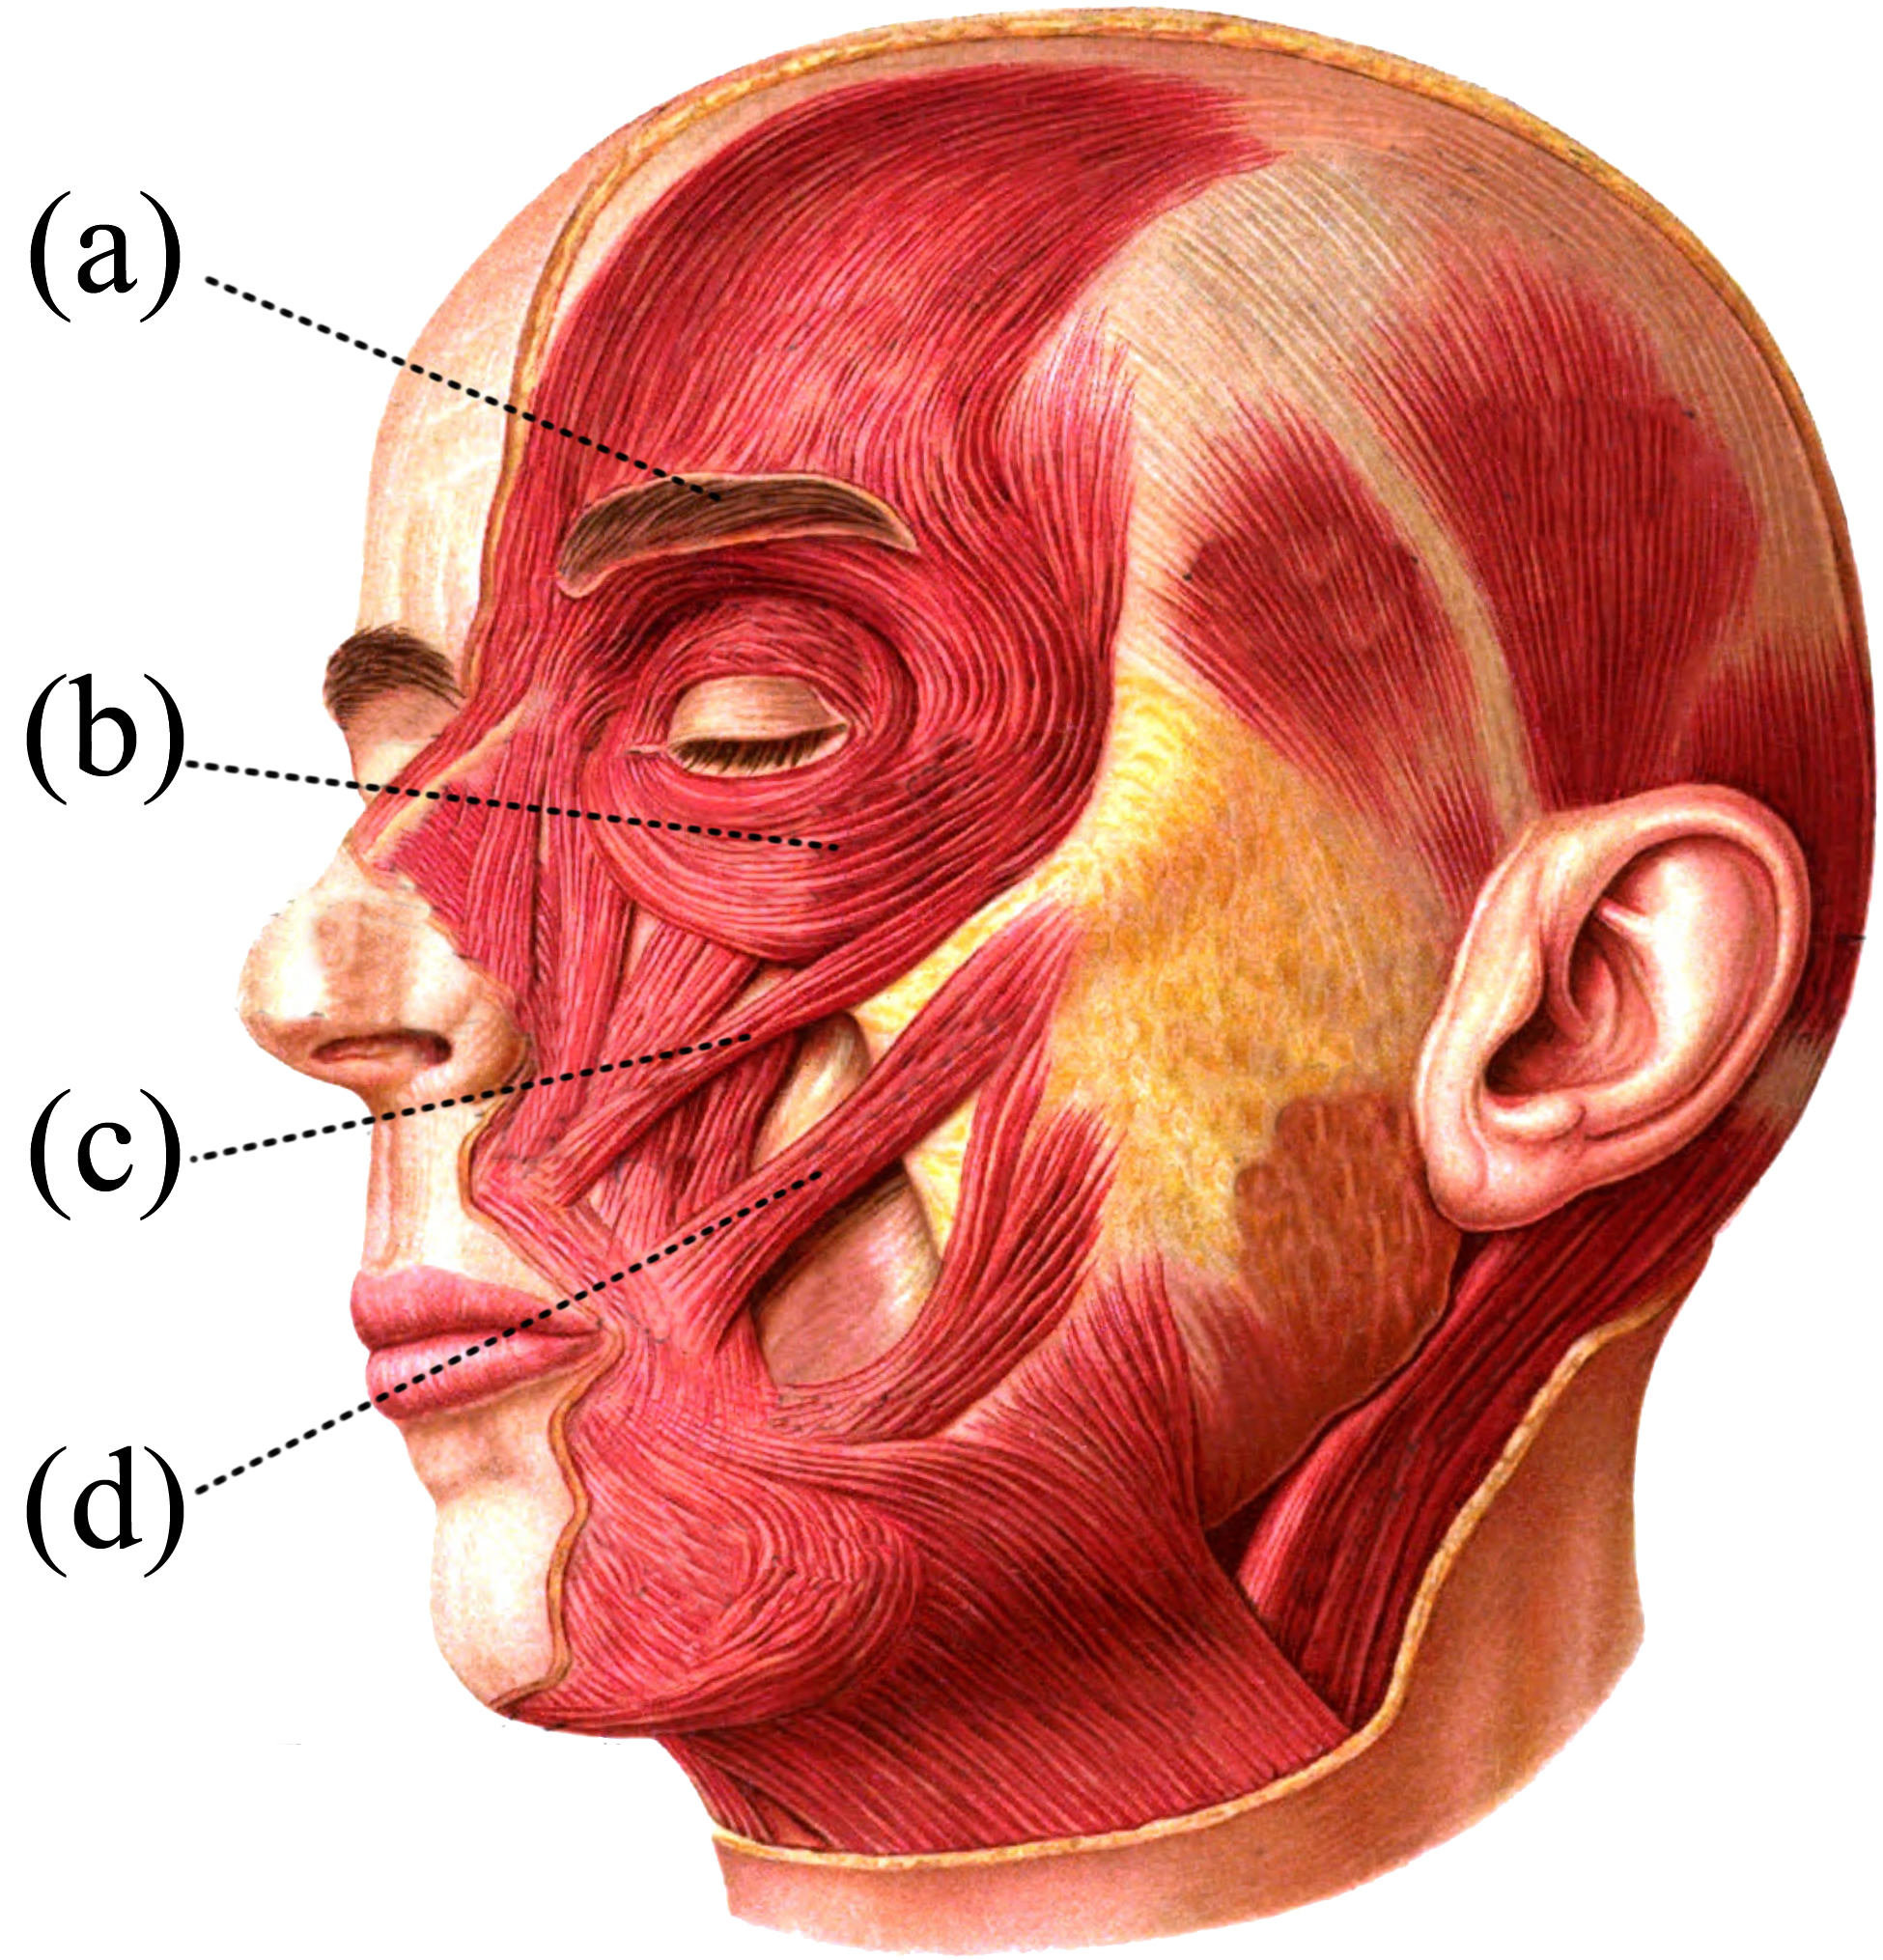
\includegraphics[width=0.8\textwidth]{Content/figures/face-muscles.jpg}
\caption{Facial muscles. (a) Corrugator supercilii. (b) Orbicularis oculi. (c) Zygomaticus minor. (d) Zygomaticus major. Adapted from ``Sobotta's Atlas and Text-book of Human Anatomy", by Dr. Johannes Sobotta (Illustration: K. Hajek and A. Schmitson), 1909. Reproduced from \parencite{sobotta1909wikimedia}.}
\label{fig:face-muscles}
\end{figure}

\textcite{hazlett2006measuring} presents evidence of more frequent corrugator activity when positive game events occur. \textcite{tijs2008dynamic} show increased activity of zygomatic muscle associated with self-reported positive emotions. Similarly \textcite{ravaja20051} show that positive and rewarding game events are connected to increase in zygomatic and orbicularis oculi EMG activity.

Approaches based on EMG are more resilient to variations of lighting conditions and facial occlusion, however they are obtrusive since physical sensors are required to be attached to the subject's face.

%%%%%%%%%%%%%%%%%%%%%%%%%%%%%%%%%%%%%%%%%%%%%%%%%%%%%%%%%%%%%%%%%%%%%%%%%%%%%%%%%%%%%%%%%%%%%%%%%%%%%%%
\section{Facial analysis based on computer vision}
%%%%%%%%%%%%%%%%%%%%%%%%%%%%%%%%%%%%%%%%%%%%%%%%%%%%%%%%%%%%%%%%%%%%%%%%%%%%%%%%%%%%%%%%%%%%%%%%%%%%%%%

Contrary to the obtrusiveness of EMG-based approaches, analysis of facial behavior based on automated visual methods can be performed remotely and without physical contact. The process usually involves the use of computer vision to perform face detection, localization of facial features (also known as landmarks or fiducial points) and classification of such information into facial expressions \parencite{salah2010communication}.

Computer vision systems usually rely on image processing, artificial intelligence, e.g. machine learning, and decision making techniques to detect and classify objects from images or videos. A class of such objects is the human face, detected and analyzed by a process called facial alignment.

\begin{figure}[h]
    \centering
    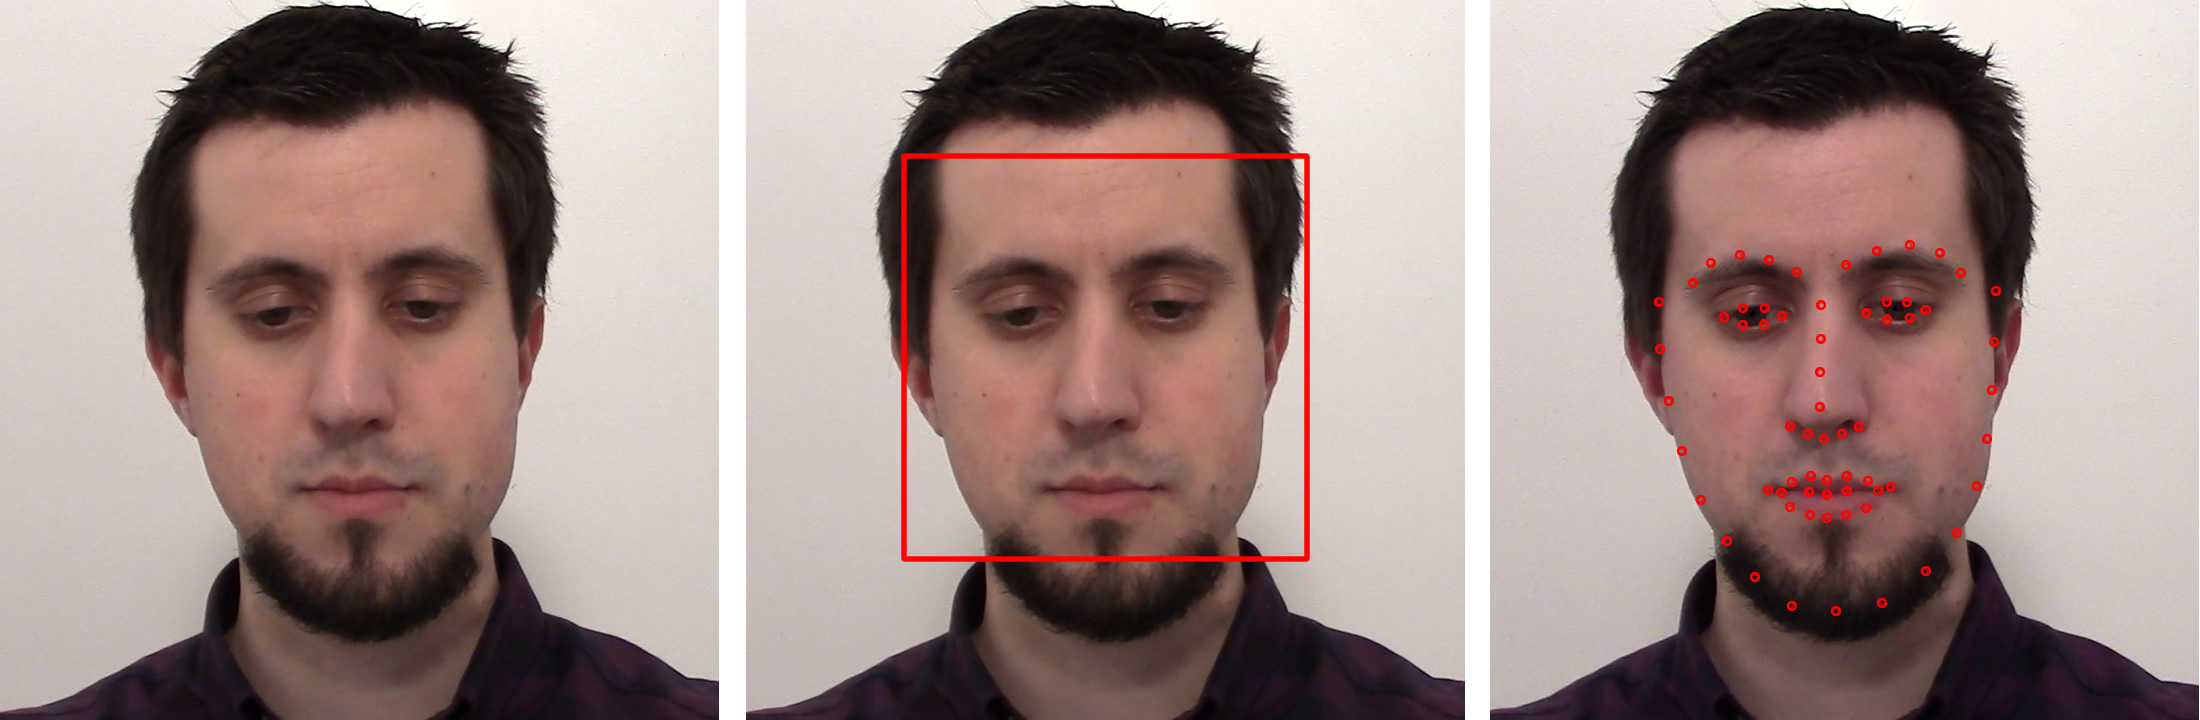
\includegraphics[width=\linewidth]{Content/figures/face-alignment.jpg}
    \caption{Example of face alignment. From left to right: input image, detected face, and aligned face.}
    \label{fig:alignment}
\end{figure}

Facial alignment consists of identifying the position of specific features of the face, e.g. eye and nose, after the face has been detected in an image/video. Figure \ref{fig:alignment} demonstrates the process. This procedure is relevant in many different scenarios, for instance facial/expression recognition and pose estimation. Research has been conducted to create accurate and fast methods that can be used to perform face alignment under an ever growing set of challenging conditions, e.g. face movement combined with different lighting configurations.

Many methods have been proposed and a literature review shows that two basic approaches are widely used in alignment techniques: constrained local models and cascaded regression methods. Both approaches work on an image of a face contained within a rectangle obtained by a face detection algorithm, such as Viola \& Jones \parencite{viola2004robust}. The following sections describe each one of them, mentioning the most relevant techniques for facial alignment that are based on the approach being described.

\subsection{Constrained Local Model}

The Constrained Local Model (CLM) approach consists of locating a set of points on a target image, then applying a constrain to them. The constrain is usually based on a statistical shape model, which is obtained via training in a set of images featuring manually inserted landmarks. Since the shape model is statistical, the position of the points (landmarks) that it describes will always resemble a face, so proportions of lines and/or the distance among points will not be so different from a human face (at least not different from the ones found in the training set). Figure \ref{fig:clm-models}(a) illustrates the configuration of the shape model with different variations.

\begin{figure}[h]
\centering
  \begin{subfigure}[b]{0.5\textwidth}
    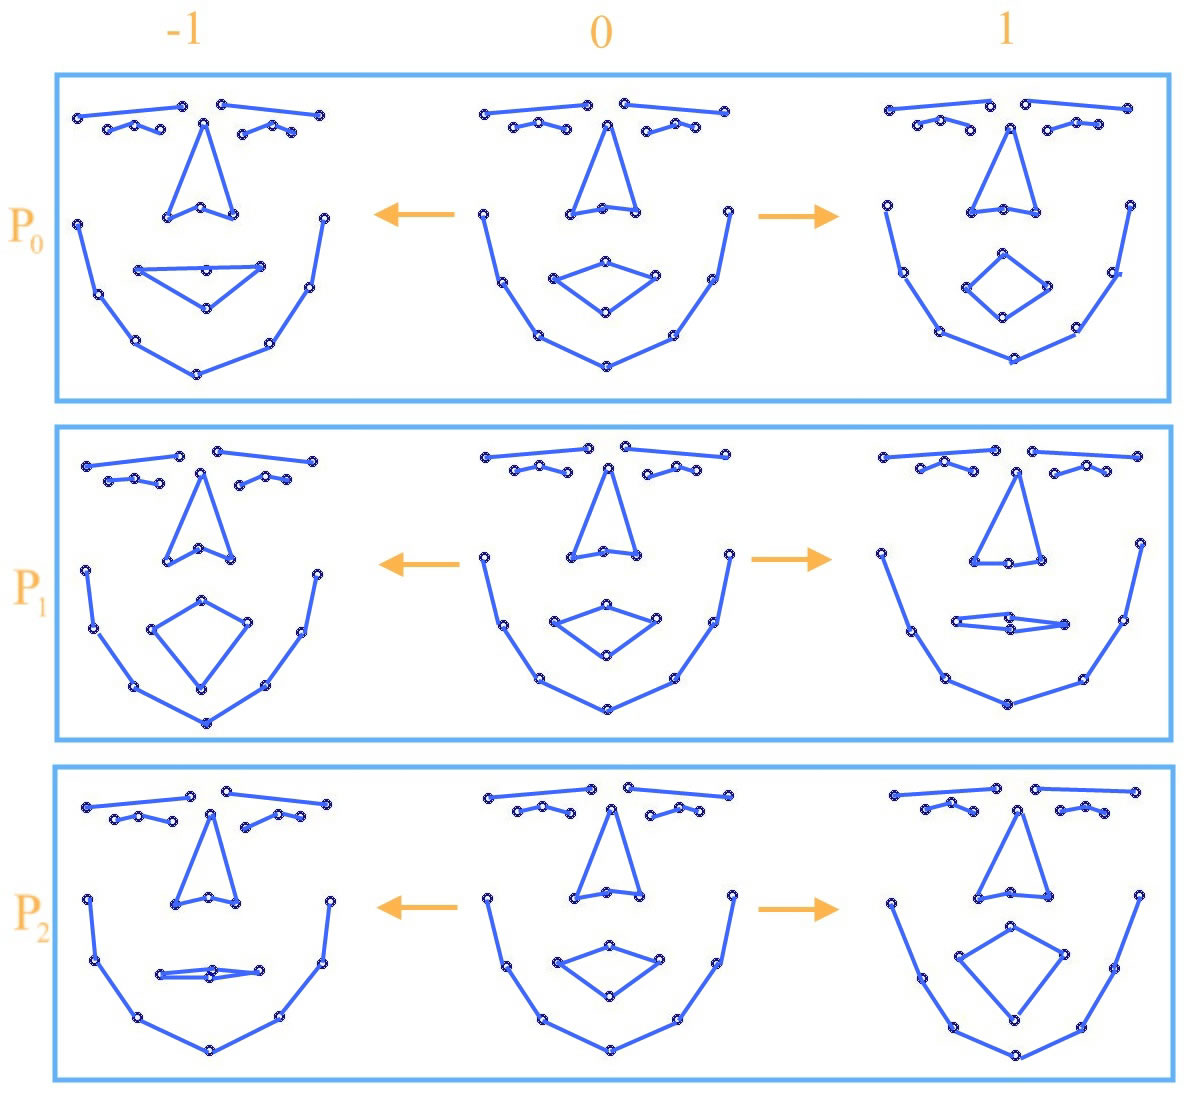
\includegraphics[width=0.95\textwidth]{Content/figures/clm-model-variation.jpg}
    \caption{}
    \label{fig:clm-model-variation}
  \end{subfigure}%
  \begin{subfigure}[b]{0.5\textwidth}
    \centering
    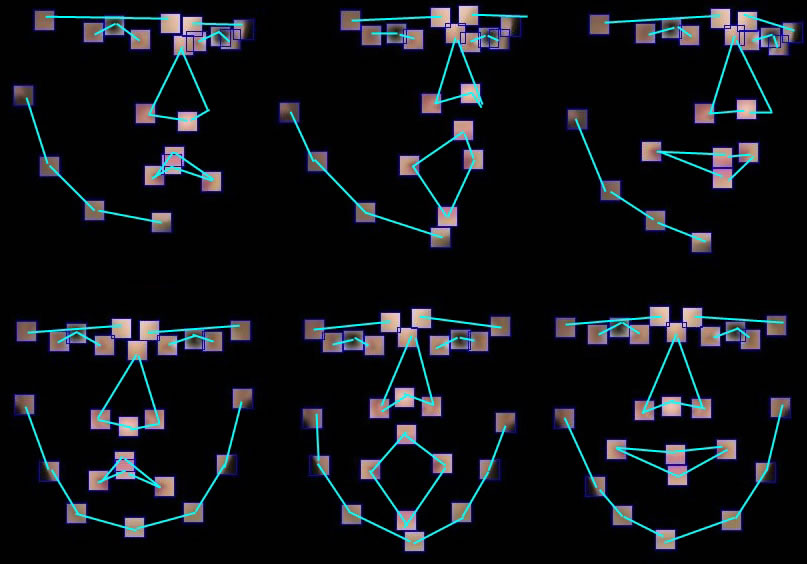
\includegraphics[width=0.95\textwidth]{Content/figures/clm-patches.jpg}
    \caption{}
    \label{fig:clm-patches}
  \end{subfigure}
  \caption{Shape models of CLM. (a) Configuration of the shape models with different variations. (b) Shape models and their respective entries in the texture model. Reproduced from \textcite{yu2010facial}.}
  \label{fig:clm-models}
\end{figure}

Additionally to the shape model, there is a texture model that contains a set of patches (images) extracted from the training images by selecting the areas around the inserted landmarks. Those patches are used to guide the search procedure in the alignment process, which allows the technique to correctly identify the right model to properly align the face being analyzed. Figure \ref{fig:clm-models}(b) shows different shape models and their respective entries in the texture model.

The process of aligning a face is iterative and it starts by sampling points that are placed in the face image according to the current shape estimation of the face. In the first try, this estimation is usually the average face obtained from all training images. The area around the sampled points are extracted and used in a search to locate a set of similar patches in the texture model. The current shape estimation and the texture patches it locates are evaluated according to a cost function. As soon as the shape variation with the minimal cost is found, the process is repeated: new patches are sampled and searched against the texture model, the current estimation is adjusted and so on. Eventually the cost function will not produce a significantly different value from one iteration to another, which means the current estimation is the best match found.

Figure \ref{fig:clm-evolution} demonstrates the evolution of the technique as it iterates in an image. First the mean shape is placed into the image and the patches are sampled around the (mistakenly) positioned landmarks. As the technique iterates, searched patches progressively induce changes in the current shape model, sampling more accurate patches. Eventually the technique converges to the aligned face.

\begin{figure}[h]
    \centering
    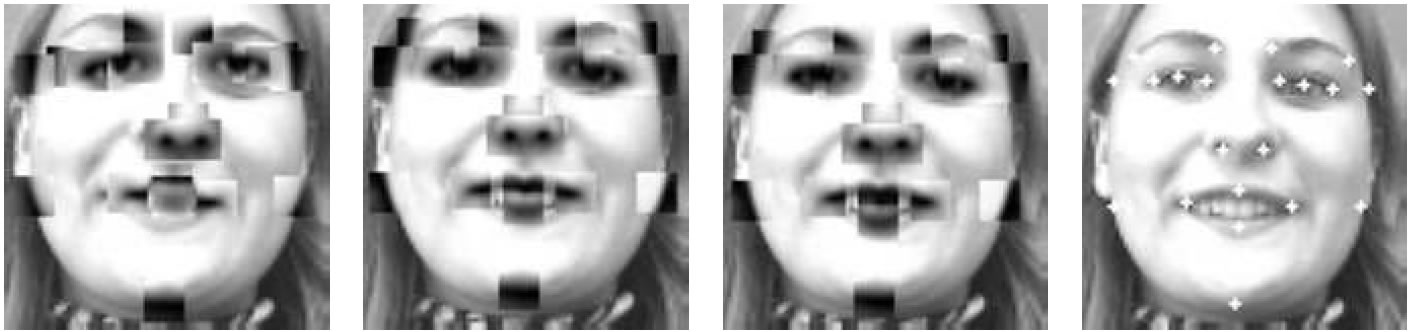
\includegraphics[width=\linewidth]{Content/figures/clm-evolution.jpg}
    \caption{Iteration of CLM during the alignment of an image. Reproduced from \textcite{cristinacce2006feature}.}
    \label{fig:clm-evolution}
\end{figure}

Two techniques that represent the CLM approach are the feature detection and tracking with constrained local models \parencite{cristinacce2006feature} and its 3D variation \parencite{baltruvsaitis20123d}, which uses 3D depth data to improve the process.

\subsection{Cascaded Regression}

The cascaded regression methods approach consists of using an initial guess shape that is progressively refined into the final answer (identification of key features in the image). This refinement is performed in a stage-by-stage manner (cascade) and the result of the current stage is used as the input for the next one. In each stage, the adjustment of the current shape (into the aligned result) is performed by a regression function, learnt via training. Early regressors in the cascade handle large variations in the shape, as opposed to the late ones, which focus on specific details. Each regressor extracts features from the image, which are then worked to produce variations in the current guess shape. The extracted features depend on the current shape and they are commonly referred as shape-indexed features.

The shape-indexed features are differences in pixel intensities. The calculation of a shape-indexed feature involves the selection of a few pixels and the subtraction of their intensities. The way those pixels are selected is usually different for each of the cascaded-regression techniques. Figure \ref{fig:shape-indexed} illustrates an example of selection of a few pixels for three particular landmarks. The landmark on the top-right (gray circle) highlights the selected pixels that will be used. The difference of intensities among those pixels will define this particular shape-indexed local feature. The shape-indexed local features are used in a decision process in each step (cascade), as illustrated by Figure \ref{fig:regressor-steps}. Usually the initial guess shape is the mean shape of the training set. This guess is used to calculate the current set of shape-indexed features to be extracted, which then guides the variation applied to the current shape. The variation to be applied is usually chosen based on the result of a cost function, which selects a variation that minimizes the distance between the current guess and the supposed aligned face. As the process repeats itself, different shape-indexed features are selected, a new variation is calculated and so on. Eventually the current shape will converge and it will represent the alignment for the face being analyzed (final shape estimation).

\begin{figure}[h]
    \centering
    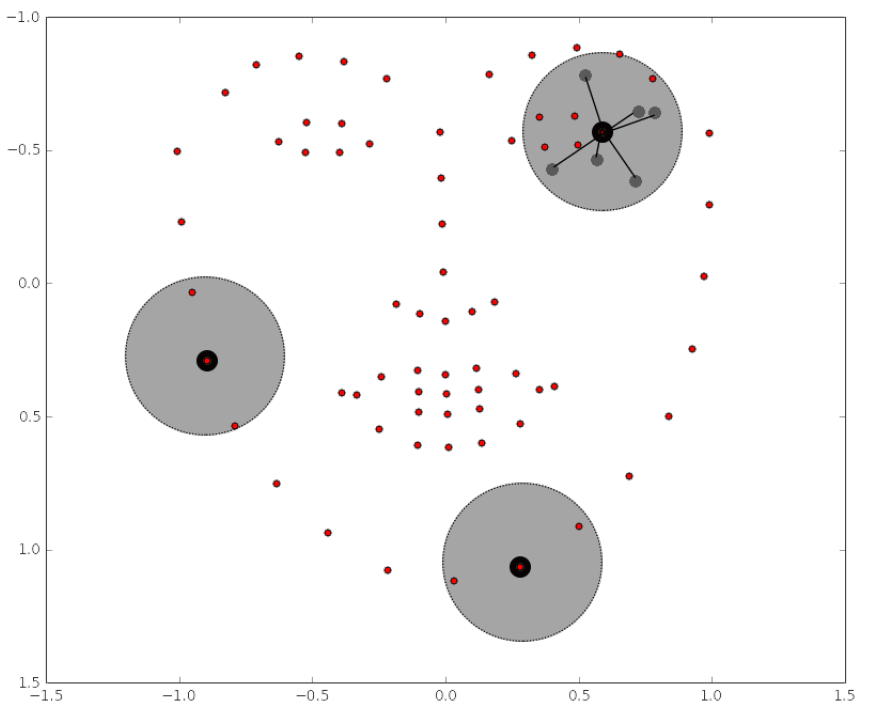
\includegraphics[width=0.6\linewidth]{Content/figures/shape-indexed.png}
    \caption{Pixels used in the calculation of a shape-indexed feature. Reproduced from \textcite{maris2015}.}
    \label{fig:shape-indexed}
\end{figure}

\begin{figure}[h]
    \centering
    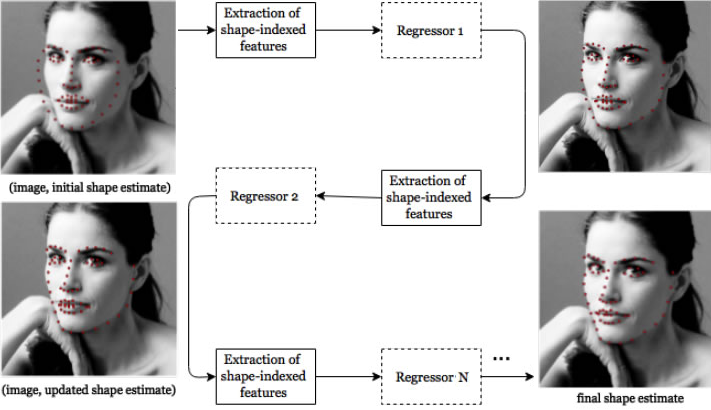
\includegraphics[width=1.0\linewidth]{Content/figures/cascade-explanation.png}
    \caption{Estimation of face shape with regressors in a set of stages. Reproduced from \textcite{maris2015}.}
    \label{fig:regressor-steps}
\end{figure}

Different variations are used to handle the training, the extraction of features and the way the regression is performed. The technique of face alignment with Ensemble of Regression Trees (ERT) \parencite{kazemi2014one}, for instance, estimates the face's landmarks by inputting the regressors with a sparse subset of pixels intensities, which is calculated with a prior probability on the distance of the pixels.

%The Supervised Descent Method (SDM) \parencite{xiong2013supervised}, on the other hand, extracts SIFT features from the current shape estimation and it converges the shape by solving a series of linear least square problems. The approach via regression of Local Binary Features (LBF) \parencite{ren2014face} proposes the use of a set of local binary features (opposed to a global view of the face) combined with a locality principle for learning and processing such features independently. Finally the face alignment by Explicit Shape Regression (ESR) \parencite{cao2014face} trains the regressors by explicitly minimizing the alignment error over training data, so all facial landmarks are regressed jointly.

%The regressors work by progressively inferring the shape, so the early regressors in the cascade handle large shape variations (ensures robustness) while later regressors focus on the small and subtle variations (ensures accuracy).

%%%%%%%%%%%%%%%%%%%%%%%%%%%%%%%%%%%%%%%%%%%%%%%%%%%%%%%%%%%%%%%%%%%%%%%%%%%%%%%%%%%%%%%%%%%%%%%%%%%%%%%
\section{Facial-based emotion detection}
\label{ch:literature-face-emotion-detection}
%%%%%%%%%%%%%%%%%%%%%%%%%%%%%%%%%%%%%%%%%%%%%%%%%%%%%%%%%%%%%%%%%%%%%%%%%%%%%%%%%%%%%%%%%%%%%%%%%%%%%%%

Facial-based emotion detection techniques try to estimate the emotional state of a subject based on the analysis of facial features. Works involving such approach commonly focus on detecting or classifying emotional states based on the six basic emotions proposed by \textcite{ekman1971constants}, i.e. happiness, surprise, sadness, fear, anger and disgust. Some visual methods rely on manual or automated FACS-based analysis as a standard for categorization and measuring of emotional expressions \parencite{bartlett1999measuring}.

The feasibility of that approach is demonstrated by \textcite{kaiser1994multi}, showing that more AU were reported by manual FACS coders during the analysis of video recordings of subjects playing the stressful part of a game when compared to its neutral part. Additionally authors report lip pull corner and inner/outer brow raise as more frequent AUs during gaming sessions. \textcite{wehrle2000emotion} also support the approach using an automated, FACS-based facial analysis aggregated with data from game events to provide an appraisal analysis of subjects emotional state.

\begin{figure}[h]
    \centering
    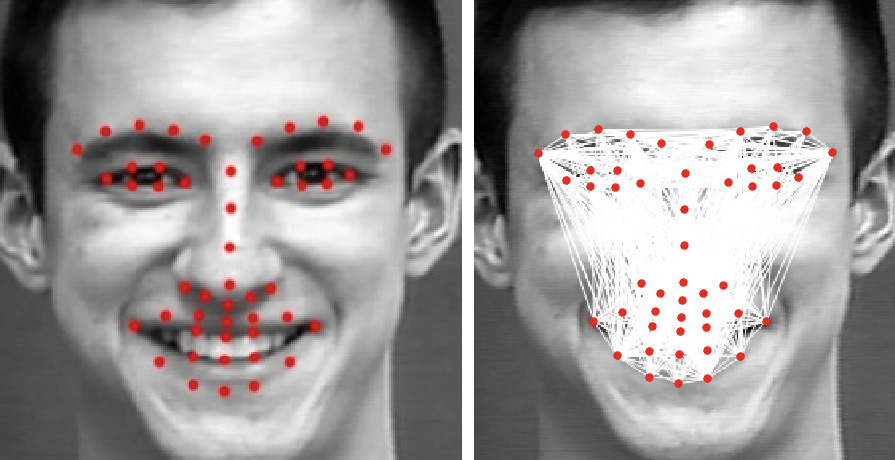
\includegraphics[width=0.75\linewidth]{Content/figures/samara2016sensing-distances.png}
    \caption{Distance-based facial feature descriptors. Left: detected facial landmarks. Right: highlight of the distance among facial landmarks. Reproduced from \textcite{samara2016sensing}.}
    \label{fig:distance-samara}
\end{figure}

Similarly \textcite{grafsgaard2013automatically} present an experiment where facial expression information is used to investigate emotional states. The experiment consists of an analysis of facial AUs during computer mediated tutoring sessions among students. Subjects and tutors interact through a tutoring software related to computer programming, while subjects are recorded. After each session, subjects answer a questionnaire related to measurements of cognitive load and engagement. The recordings are analyzed in an automated way with manual verification of the results. A predictive model is constructed using the questionnaire answers and the recording analysis, which results in correlations of facial AU and emotional states. The authors compare their findings against other research, which differ significantly. For instance, brow lowering has been correlated with confusion in previous work, however the authors found that it was a positive predictor of student frustration in the context of their experiment.

\textcite{heylen2005facial} also present a similar investigation in a pilot experiment of a tutoring session related to the application of subcutaneous injection. Students interact with a virtual patient while using a physical haptic device to administrate an injection. The recordings of the students are analyzed by the researchers to make annotations of the expressions based on their own interpretation of the context. The researchers use a compilation of literature components to guide the evaluation of the collected data. As the authors point out, a variety of expressions occur, but most of the time students remain with a neutral facial expression. The annotated features are (ordered from most to less frequent): smile (total 22), raise eyebrows (11), pull down mouth corners (2) and frown (1).

%As opposed to previously mentioned works, our approach consists of using induced boring to stressful mechanics in games to produce variations in the emotional state of participants. Our experiment has a linear progression from a boring to a stressful state that should be perceived by the subjects. We believe such configuration gives our experiment a novel approach for the exploration of facial actions and HR regarding their connection to emotional states, since we can categorize information according to the induced (and theoretically known) emotional states. To the best of our knowledge, this is the first experiment where games with linear boring-to-stressful progression are used to deliberately induce emotional reactions.

Differently than the previously mentioned works, other initiatives aim to detect emotions based on the analysis of facial landmarks and their distances, movement or angles. \textcite{joho2009exploiting} use facial analysis for affective video summarisation. The authors use an automated face tracking approach to obtain a vector of motion features of certain regions of the face, named Motion Units (MU). MUs are classified by a Bayesian network, which is trained from labeled data. Results indicate promicing correlation between the manually annotated content of the videos and the automatically classified one.

Somewhat similarly \textcite{akakin2010spatiotemporal} detect facial landmarks over consecutive frames of videos, whose trajectories (time series) during head gestures and facial expressions are organized in a spatiotemporal matrix. Discriminative features are extracted from the trajectory matrix, which are used to train machine learning models, i.e. Adaboost and SVM. Classification accuracy is reported to be around 90\% for the detection of 7 face and head gestures in a datased composed of 210 videos of 4 subjects). The detection of emotions, however, is limited to only two states, i.e. hapiness and sadness.

Finally \textcite{samara2016sensing} present the sensing of affective states based on the analysis of the distances of facial landmarks. Automated face detection is employed to detect facial landmarks, however no coding scheme is used to identify the detected points. Instead the authors use the Euclidian distance among facial landmarks, represented as distance vectors, to train a SVM model to detect expressions. Figure \ref{fig:distance-samara} illustrated the process. Detection accuracy is improved by a two-state SVM classification model, entitled by the authors as Hierarchical Parallelised Binary Support Machines. Accuracy rates of about 96\% were achieved on two facial expression datasets. \textcite{samara2016sensing} alse use the Euclidean distance among face points to train a Support Vector Machine (SVM) model to detect expressions. Similarly \textcite{chang2009emotion} use 12 distances calculated from 14 landmarks to detect fear, love, joy and surprise. \textcite{hammal2007facial} use 5 facial distances calculated from lines in key regions of the face derived from the MPEG-4 animation standard \parencite{abrantes1999mpeg}, e.g. eyebrows, for classification of expressions. \textcite{tang20083d,tang2008line} use up to 30 Euclidean distances among facial landmarks also obtained from MPEG-4 based 3D face models to recognize the 6 universal facial expressions. Similarly \textcite{hupont2013facial} classify the same emotions by using a correlation-based feature selection technique to select the most significant distances and angles of facial points.

The use of facial expressions as a single source of information, however, is contested in the literature. \textcite{blom2014towards} report that subjects present a neutral face during most of the time of gameplay and frustration is not captured by face expressions, but by head movements, talking and hand gestures instead. In a similar conclusion, \textcite{shaker2011game} show that head expressivity, i.e. movement and velocity, is an indicator of how experienced one is on games. Additionally high frequency and velocity of head movements is indicative of failing in the game.

%%%%%%%%%%%%%%%%%%%%%%%%%%%%%%%%%%%%%%%%%%%%%%%%%%%%%%%%%%%%%%%%%%%%%%%%%%%%%%%%%%%%%%%%%%%%%%%%%%%%%%%
\section{Summary}
\label{sec:literature-face-summary}
%%%%%%%%%%%%%%%%%%%%%%%%%%%%%%%%%%%%%%%%%%%%%%%%%%%%%%%%%%%%%%%%%%%%%%%%%%%%%%%%%%%%%%%%%%%%%%%%%%%%%%%

Facial analysis based on physical sensors, e.g. EMG, provide continuous monitoring of subjects and are not affected by lighting conditions or pose occlusion by subject's movement. However they are obtrusive and the use of sensors increase user's awareness of being monitored \parencite{yamakoshi2007preliminary,yamaguchi2006evaluation,healey2005detecting}. Approaches based on video analysis, e.g. FACS and computer vision, are less intrusive. Despite the fact that FACS has proven to be a useful and quantitative approach for measuring facial expressions \parencite{bartlett1999measuring}, its manual application is laborious, time-consuming and requires certified coders to inspect the video recordings. The application of FACS also has downsides, including different facial expression decoding caused by misinterpretation in specific cultures \parencite{jack2013culture}.

Facial analysis from visual methods, such as the previously mentioned feature-based approaches relying on computer vision, are quicker and easier to deploy. Automated facial analysis as a mean to detect the emotional state of players has been proved to work at creating emotionally adapted games \parencite{saari2004towards} or tools for unobtrusive game research. When automated facial analysis is used, it is often tested on contexts not related to games, or facial cues are derived from models not designed for analysis of emotional interactions in games, such as the MPEG-4 standard \parencite{abrantes1999mpeg}. Such standard specifies representations for 3D facial animations, not emotional interactions in games. Automated facial analysis is also commonly performed on images or videos whose subjects are acting to produce facial expressions, which are likely to be exaggerated in nature and not genuine emotional manifestations. Those are artificial reactions that are unlikely to happen in a context involving subjects interacting with real games, where emotional involvement between subject and game is stronger. Another limitation of previous work is the common focus on detecting facial expressions \textit{per se}, e.g. 6 universal facial expressions \parencite{ekman1971constants}, not necessarily detecting isolated facial actions, e.g. frowning, associated with emotional reactions in games. Finally people are different and elements as age and familiarity with a game influence the outcome of automated facial analysis of behavioral cues \parencite{asteriadis2012towards}, as well as different games might induce different bindings of facial expressions \parencite{tan2014correlation}. Empirical results of manual annotations of facial behavior in gaming sessions have indicated more annotations during stressful than during boring (see Section \ref{sec:experiment1-study1}) or neutral \parencite{kaiser1994multi} parts of games. As a consequence, a more user-tailored contextualization is essential for any study involving facial analysis, particularly involving games.

%Further investigation of such findings using an automated analysis instead of a manual approach is a topic of interest for game researchers and practitioners, who can benefit from improved tools related to facial behavior analysis.

%However previous works commonly focus on analyzing images or videos whose subjects performed facial expressions on guidance. Those are artificial circumstances that do not portrait natural interactions of users and games, for instance. When the analysis is performed on videos of subjects interacting with games, usually the aim is to detect a very specific set of facial expressions, e.g. 6 universal facial expressions, disregarding head movement and subtle changes in facial behavior.

%Such difference in results is expected due to the variational nature of facial expressions among different individuals and contexts, however it underlines the complexity of correlating facial features and emotions

\chapter{Emotions and physiological signals}
\label{ch:literature-physiological}

The empowerment of computers with the understanding of emotions is one of the focus of human-computer interaction research. The use of physiological signals of users in the process of detecting emotions involves the different input signals, such as electrocardiogram data, skin temperature and electro-dermal activity, among others. A significant number of works explore such inputs and the challenges associated with them on emotion recognition using physiological signals \parencite{jerritta2011physiological}.

% TODO: add Thesis - AIZoubi, page 62 (paper) or 79 (digital PDF indicator).
% TODO: add table info from Thesis - AIZoubi, page 45 (paper) or 62 (digital PDF indicator).

\begin{table}[h]
\caption{Most common psychophysiological measurements used in human interaction studies \parencite{jerritta2011physiological}}
\label{table:physiological-signals}
\begin{tabular}{L{.4\linewidth}L{.5\linewidth}}%
\toprule%
\textbf{Respiratiry system} & Breaths per minute\\
 & Respiration volume \\
\midrule
 \textbf{Electrodermal activity} & Skin conductance (SC) \\
 & Galvanic skin response (GSR) \\
\midrule
\textbf{Brain activity} & Electroencephalography (EEG) \\
& Brain imaging methods \\
\midrule
\textbf{Muscular system} & Electromyography \\
\midrule
\textbf{Cardiovascular system} & Heart rate variability (HRV) \\
& Respiratory Sinus Arrhythmia (RSA)  \\
& Cardiact output  \\
& Inter beat interval (IBI) \\
& Blood pressure (BP)  \\
\bottomrule%
\end{tabular}%
\end{table}

One of the reasons why physiological signals are interesting for emotion recognition is because suppressing emotions or social masking through physiological signals is impossible \parencite{kim2004emotion}. In the games research field, there have been studies aiming at using such theory and psychophysiological methods applied to game research \parencite{kivikangas2011review}. It has been demonstrated that it is possible to use physiological signals to automatically assess different emotional states in the context of games using a variety of signals \parencite{bousefsaf2013remote,yun2009game,rani2006empirical,tijs2008dynamic}.

Different approaches exists for emotion elicitation stimuli, feature extraction and classification methodologies regarding emotion recognition. Table \ref{table:physiological-signals} presents the most common psychophysiological measurements used in human interaction studies. The aim of this thesis is to remotely obtain physiological information from users to detect emotional states. As a consequence, the input signals presented in Table \ref{table:physiological-signals} were researched and filtered based on the existence of techniques that are able to remotely measure them. HR was identified as a reliable physiological signal regarding emotion detection which can be remotely estimated via video of subjects. HR has been used to measure emotional states \parencite{kivikangas2011review}, including the detection of emotions as stress \parencite{choi2009using} and boredom \parencite{yamakoshi2007preliminary}. Additionally computer games were proven to provoke alteration in the mean HR of players at stressful periods of gameplay \parencite{sharma2006assessment,rodriguez2015vr}.

The following sections present more details regarding the physiology of HR and its use in emotion detection.

%Multimodal sensing consists of reading different signal channels from a subject. A person presents a wide set of those channels, such as blood pressure, pulse oximetry, facial expressions, pupillary variation, among others. The analysis of such data can be used to infer the subject's emotional/stress state, for instance. Usually biometric sensors attached to the subject are used to read the channels, however remote approaches are proving to be feasible. The following subsections present some of those channels and the sensing techniques used to extract them. All of them are non-intrusive, working by analyzing a video of the subject with no physical contact.

%In games research, quantitative approaches already used HR to measure engagement \parencite{ravaja20051}, for instance.
%there are initiatives to measure such states and other elements, such as engagement/immersion \parencite{boyle2012engagement} and presence \parencite{weibel2011immersion}.

%%%%%%%%%%%%%%%%%%%%%%%%%%%%%%%%%%%%%%%%%%%%%%%%%%%%%%%%%%%%%%%%%%%%%%%%%%%%%%%%%%%%%%%%%%%%%%%%%%%%%%%
\section{Physiology of heart rate}
%%%%%%%%%%%%%%%%%%%%%%%%%%%%%%%%%%%%%%%%%%%%%%%%%%%%%%%%%%%%%%%%%%%%%%%%%%%%%%%%%%%%%%%%%%%%%%%%%%%%%%%

The cardiac cycle is periodic and it contains a set of waves that reflect depolarization and repolatization events, which are all connected to the functioning mechanism of the heart \parencite{yanowitz2012introduction}. Figure \ref{fig:rr-interval} illustrates two cardiac cycles with highlights on each of such waves. The X axis represents time in milliseconds and the Y axis represent the wave amplitude. A heartbeat is a contraction and relaxation of the heart, which is connected to the Q, R and S waves, known as the QRS complex.

\begin{figure}[h!]
    \centering
    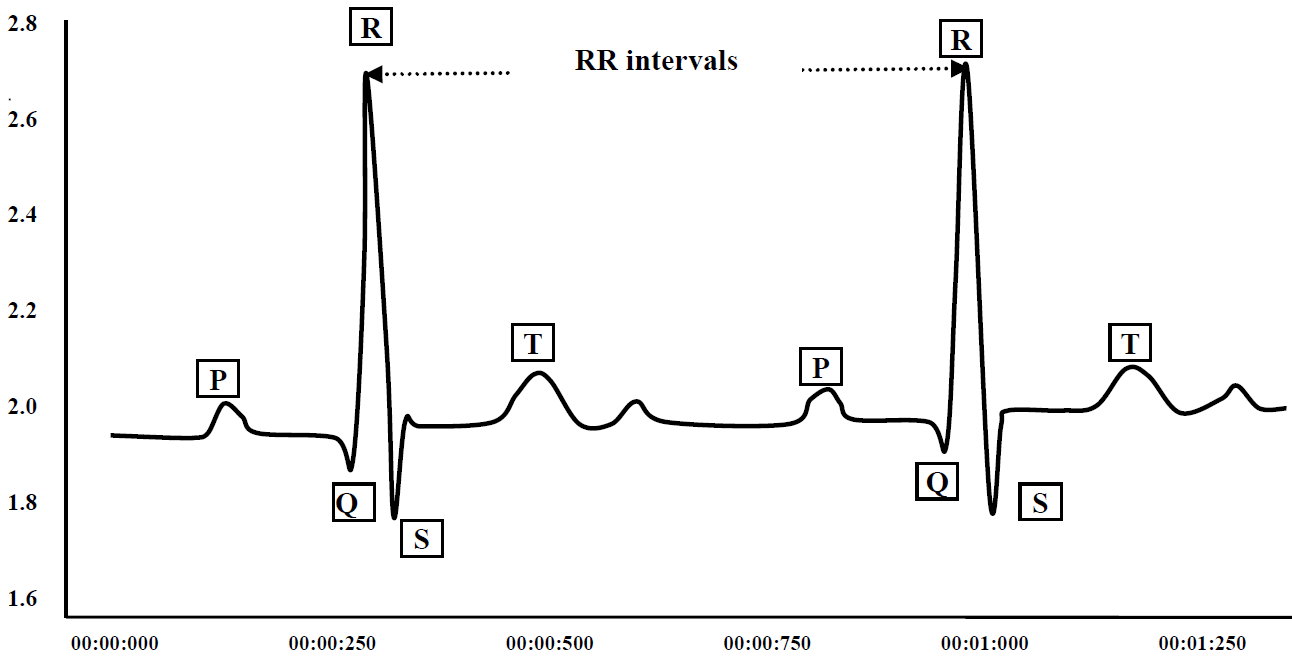
\includegraphics[width=1.0\linewidth]{Content/figures/rr-interval.png}
    \caption{Two cardiac cycles with highlights on each its electrical waves. The X axis represents time in milliseconds and the Y axis represent the wave amplitude. A heartbeat is connected to the Q, R and S waves, known as the QRS complex. Reproduced from \textcite{ahmed2010heart}.}
    \label{fig:rr-interval}
\end{figure}

The tracing of the QRS complex allows the monitoring of the heart rate. The peak of the R wave, referred to as R peak, marks an specific time in the cardiac cycle. The difference between two R wave peaks is the RR interval, also known as inter-beat interval (IBI). The RR interval reflects the entire duration of each heart beat. As a consequence, the amount of R waves within one minute is used to calculate the HR. The variations in time between R peaks, which is the beat-to-beat variability of HR, is referred to as heart rate variability (HRV).

The HR is connected to the central nervous system and it can be influenced by a series of different elements, including modifiable and non-modifiable ones \parencite{valentini2009variables}. Modifiable elements are those related to external influence, such as mental stress or physical activity. Non-modifiable elements are related to physiology, such as age, gender and race. A healthy human adult has a HR within the interval of [45 bpm, 240 bpm], the equivalent of [0.75 Hz, 4 Hz] \parencite{li2014remote}.

% A healthy human adult has a HR between 45 - 240 bpm (0.75 - 4 Hz) [1]. There are many factors influencing the HR of a person, both modifiable (e.g. physical activity, mental stress, smoking) and non-modifiable (e.g. age, gender) [12]. The HR can change rapidly from activities such as postural changes [13] and also from uncontrolled events such as cardiac arrhythmia and sudden cardiac arrest [14, 15].

% [1] X. Li et al. “Remote Heart Rate Measurement from Face Videos under Realistic Situations”. In: Computer Vision and Pattern Recognition (CVPR), 2014 IEEE Conference on. June 2014, pp. 4264–4271. doi: 10.1109/CVPR.2014.543
%
% [12] M. Valentini and G. Parati. “Variables Influencing Heart Rate”. In: Progress in Cardiovascular Diseases 52 (2009), pp. 11–19
%
% [13] C. Borst et al. “Mechanisms of initial heart rate response to postural change”. In: American Journal of Physiology - Heart and Circulatory Physiology 243.5 (1982), H676–H681
%
% [14] National Heart, Lung and Blood Institute. How Is Sudden Cardiac Arrest Diagnosed? http://www.nhlbi.nih.gov/health/health-topics/topics/ scda/diagnosis. Accessed: 2016-06-02

%%%%%%%%%%%%%%%%%%%%%%%%%%%%%%%%%%%%%%%%%%%%%%%%%%%%%%%%%%%%%%%%%%%%%%%%%%%%%%%%%%%%%%%%%%%%%%%%%%%%%%%
\section{Heart rate, stress and frustration}
%%%%%%%%%%%%%%%%%%%%%%%%%%%%%%%%%%%%%%%%%%%%%%%%%%%%%%%%%%%%%%%%%%%%%%%%%%%%%%%%%%%%%%%%%%%%%%%%%%%%%%%

The foundation of HR-based approaches for emotional estimation draws on the theory that physiological signals are linked to emotion regulation \parencite{appelhans2006heart,fenton2012emotion,schubert2009effects}. The automatic nervous system (ANS), a key system in the generation of physiological arousal \parencite{appelhans2006heart}, is subdivided into the sympathetic nervous system (SNS) and the parasympathetic nervous system (PNS). Those systems interact (often antagonistically) to produce variations in the physiological signals to prepare a person to react to a situation. The SNS is dominant during physical and psychological stress, triggering the body to alertness, increasing HR, for instance. This is commonly referred to as ``fight or flight'' response. The PNS, on the other hand, is dominant in periods of stability and relative safety, maintaining physiological signals at a lower degree of arousal, e.g. decreasing HR. The continuous changes between SNS and PNS impulses cause variations of HR and HRV \parencite{schubert2009effects}, which refers to beat-to-beat alternations in HR intervals.

Physiological signals, such as HR, are hard to fake because of their link with the ANS, differently from facial expressions \parencite{Landowska}, for instance. As a consequence, HR and its derivatives, such as HRV, have been used as reliable sources of information in different emotion estimation methods \parencite{kukolja2014comparative}. Additionally it has been used as an indication of perceived interest and confusion in mobile applications \parencite{xiao2015towards}, as player input for games \parencite{stockhausen2013beats}, and as triangulation of phychophysiological emotional reactions to digital media stimuli \parencite{nogueira2015annotation}. The significant variation of physiological signals, however, is an obstacle to its use in emotional estimation. Signals increase during emotional arousal, but decrease in response to attention engagement, which makes the measurement of engagement, for instance, a non-trivial process \parencite{ravaja20051}. Despite such challenges, the use of HR and HRV has been demonstrated in a continuous arousal monitor \parencite{grundlehner2009design} as well as a detection mechanism for mental and physical stress based on physical and mental tasks \parencite{vandeput2009heart,garde2002effects}. Results indicate higher HR during the mentally demanding task when compared to the rest period. The HR mean alone also has been shown to be a measurement of frustration in a game \parencite{rodriguez2015vr}.

%As previously mentioned, however, the use of sensors that require physical contact might disturb the user experience or be sensitive to noise. Even when users state they forgot about the use of physical sensors during a gaming session, researchers still face noisy data due to subject motion affecting the sensors \parencite{brogni2006variations}.

\textcite{vandeput2009heart} demonstrate the use of HR and HRV to detect mental and physical stress. Three demanding activities (a postural task, a mental task and a task that is a combination of both) are used and for almost all HR measures obtained, the demanding activities can be distinguished from the rest period. The authors also point out that mental stress decreased high frequency components of the HRV interval (i.e. $HRV_{HF}$), while increasing low frequency ones (i.e. $HRV_{LF}$). A similar experiment was conducted by \textcite{garde2002effects} involving two tasks: one being mental and physically demanding (digital version of the Stroop color word test \parencite{golden1978stroop}) and other being only physically demanding. The authors confirm the findings of \textcite{vandeput2009heart} by showing higher HR, increased $HRV_{LF}$ and decreased $HRV_{HF}$ during the mentally demanding task when compared to the rest period.

\textcite{bousefsaf2013remote} also use a digital version of the Stroop test in a similar experiment. A combination of HR, HRV and HRV\textsubscript{HF} is used to estimate the stress state of subjects. The resulting stress state curve tends to decrease during the rest period and increase during stress sessions (as did the HR), in accordance with the previously mentioned works; additionally the self-reported answers to questionnaires present significant differences of stress level in the rest and in the stress sessions as well. \textcite{mcduff2014remote,mcduffcogcam} also use HR and its variants in order to measure cognitive stress during computer tasks. According to the authors, the average heart rate and breathing rate are not significantly different in any case, which differs from the findings of previously mentioned work. The variations of HRV\textsubscript{LF} and HRV\textsubscript{HF}, however, are significantly different during the cognitive tasks compared to the rest period; higher HRV\textsubscript{LF} and lower HRV\textsubscript{HF} power are found in both cognitive tasks compared to the rest period, which aligns with findings of previous work. Stress predictions made by the model are consistent with the self-reported answers provided by subjects.

\textcite{grundlehner2009design} present a real-time, continuous arousal monitor. Using a wireless sensor network for signal acquisition, the authors record and use four signals from subjects to estimate arousal: electrocardiogram (ECG), respiration, skin conductance and skin temperature. The ECG is used to calculate HRV, which is then used in the estimation. A regression analysis is performed to identify the importance of the features in the estimation of arousal. HRV\textsubscript{LF} and HRV\textsubscript{HF} are not significant when compared to the other signals (e.g. skin conductance), while the standard deviation of HRV presents a significant weight. The arousal prediction matches the hypothesized arousal events marked by the authors in each of the experiment parts (e.g. start of noise in the audio part).

% TODO: add \cite{anttonen2005emotions,witvliet2007play}

\chapter{Remote photoplethysmography: non-contact heart rate measurement}
\label{ch:literature-rppg}

Photoplethysmography (PPG) is a technique commonly used to measure HR based on the variations of light absortion in the human skin. The pressure of the cardiac activity causes the blood vessels to change volume and light absorbtion rate because of the levels of oxigen in the blood flow. Such differences make the light absorption on the skin surface change accordingly. PPG is a time-varying signal resulted from such differences in the light absorption in live human tissue, which can be processed to calculate the HR. The process is illustrated in Figure \ref{fig:ppg}. The employment of PPG requires a physical sensor, e.g. finger pulse oximeter, in order to be performed.

\begin{figure}[h]
\centering
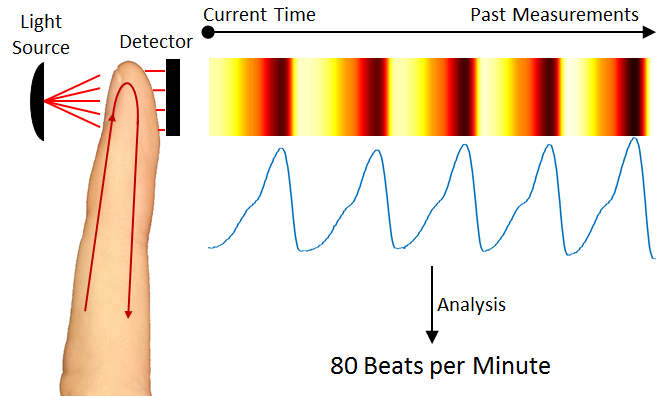
\includegraphics[width=0.7\linewidth]{Content/figures/ppg.png}
\caption{General structure of a physical photoplethysmographic system. Adapted from \textcite{chwyl2016statistical}.}
\label{fig:ppg}
\end{figure}

Further research on PPG \parencite{mcduff2015survey} evolved the technique to allow it to be performed remotely based on the analysis of a video of a person. The remote approach is commonly refered in the literature as remote photoplethysmography (rPPG)  \parencite{allen2007photoplethysmography}. Such improvement removed the requirement of a physical sensor or any physical contact for the estimation of HR and its derivates. A literature review shows the existence of a variety of different rPPG approaches, including thermal-, image-, and movement-based ones \parencite{kranjec2014non, Sereevoravitgul}. The following sections present the common structure of an rPPG technique, a survey of existing rPPG techniques and information regarding accuracy and limitations of such technology.

%rPPG-based methods for HR measurement are tools that can be used by the HCI community, particularly in games research.

%The use of physiological signals to infer information about users is a recurrent research topic \parencite{kivikangas2011review,jerritta2011physiological, kukolja2014comparative}. However the methods employed to obtain such signals are commonly based on physical contact, e.g. ECG, and few initiatives have been carried out relying on non-contact approaches, e.g. rPPG. In the computer vision domain, on the other hand, an increasing number of works is concerned with creating new (or improving already existing) techniques for rPPG. To provide an introduction for readers unfamiliar with rPPG, we introduce its general structure and the core techniques in the field. Additionally we present works involving physiological signals, in particular HR, and game-related materials commonly used for detection of emotional states of users.

%%%%%%%%%%%%%%%%%%%%%%%%%%%%%%%%%%%%%%%%%%%%%%%%%%%%%%%%%%%%%%%%%%%%%%%%%%%%%%%%%%%%%%%%%%%%%%%%%%%%%%%
\section{Structure of the technique}
\label{sec:literature-rppg-structure}
%%%%%%%%%%%%%%%%%%%%%%%%%%%%%%%%%%%%%%%%%%%%%%%%%%%%%%%%%%%%%%%%%%%%%%%%%%%%%%%%%%%%%%%%%%%%%%%%%%%%%%%

There exist initiatives to classify \parencite{rouast2016remote, mcduff2015survey} and formally model the algorithmic principles \parencite{Wang_2016algorithmic} of rPPG techniques. In that light, \textcite{rouast2016remote} propose a general algorithm framework composed of three phases that are common to all rPPG techniques (see Figure \ref{fig:rppg}): signal extraction, signal estimation and heart rate estimation.

\begin{figure}
\centering
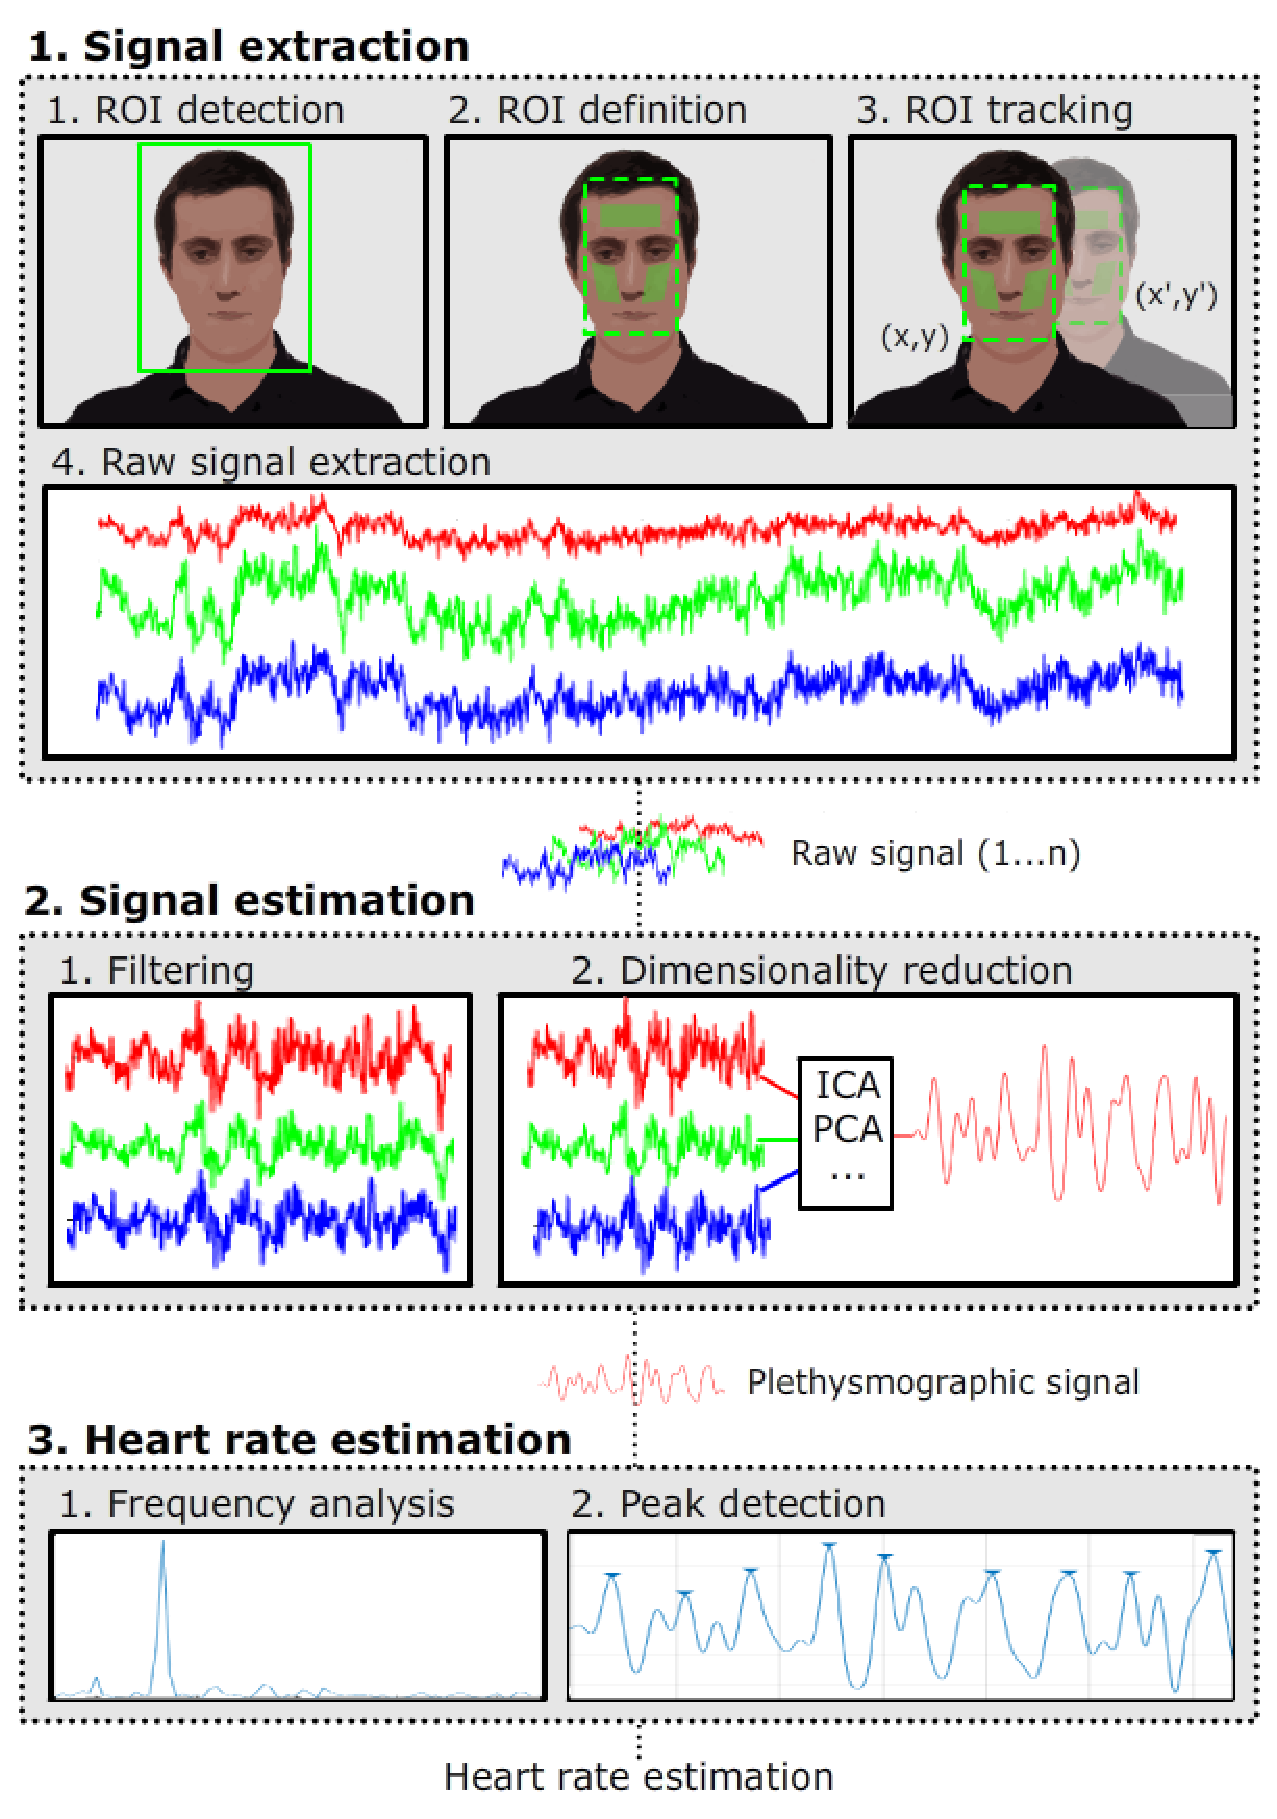
\includegraphics[width=0.9\linewidth]{Content/figures/general-rppg}
\caption{General algorithm framework common to all rPPG techniques. Adapted from \textcite{rouast2016remote}.}
\label{fig:rppg}
\end{figure}

\subsection{Signal extraction}

The signal extraction phase extracts a set of raw signals from a video. Step 1 relates to the detection of a region of interest (ROI), which is an area of the video that usually contains the face of the subject. Approaches commonly used for this step are the algorithm of Viola\&Jones (VJ) \parencite{viola2004robust}, a machine learning based approach to classifying faces, Active Appearance Models (AMM) \parencite{EdwardsAAM} and facial landmark detectors. %\parencite{saragih2011deformable,martinez2013local}.

In step 2 (ROI definition) the parts of the ROI to be used for the signal extraction are defined. Approaches commonly employed include the use of whole ROI (usually the bounding box returned by VJ, which is likely to contain background pixels along with the facial pixels), a part of the ROI (e.g. 60\% of the bounding box width) or specially defined areas (e.g. forehead, cheeks or shapes defined by facial landmark points).

Step 3 (ROI tracking) deals with the process of tracking the defined ROI area over the duration of the video. Ideally the PPG signal should be extracted from the pixels belonging to the same skin region over time. This is unlikely to happen due to subject motion, be it voluntary or not (subjects will present movement that influences the ROI even when still \parencite{poh2010non}). A common approach for this step is the re-detection of the ROI for each frame, which is computationally suboptimal and still prone to noise. Detection algorithms, e.g. VJ, are not likely to be exact, so results between consecutive frames might be slightly different, which causes fluctuation in the defined ROI. More elaborated approaches avoid the costly frame-by-frame re-detection procedure (and its fluctuations) by updating an already detected ROI in subsequent frames. The update is based on movement information obtained from tracking algorithms applied to features/points within the ROI. %Examples of such algorithms are Good Features to Track, Kanade-Lucas-Tomasi (KLT), Speeded Up Robust Features (SURF), Kernel-based Object Tracking and tracking-by-detection with kernels.

Finally in step 4 (raw signal extraction) a raw (untreated) signal is extracted. It is a time-varying signal whose points/samples are obtained from the content of the defined ROI in each frame of the video. One common approach used to extract the signal is based on colors, e.g. average of the values of the pixels of each channel (R, G and B) over time produces the raw signal. Another approach is based on the movement of the head, which is a mechanical reaction to the blood flow in the aorta. Feature points within the defined ROI are tracked over time by a tracking algorithm and the horizontal and/or vertical variations in the trajectory of the points produce the raw signal. The signal extraction phase can result in multiples raw signals, which are dependent on the approach applied. A color-based approach, for instance, might result in three raw signals, one for each color channel (RGB).

\subsection{Signal estimation}

The raw signals are filtered and combined to produce a single estimated plethysmographic signal. The filtering step aims to remove unwanted noise from the raw signal, which could be caused by the capturing device (e.g. camera noise), subject movement, changes in illumination, etc. The raw signal is usually normalized (subtracted by its mean and divided by its standard deviation) first. The commonly used filters are based on high/low pass, such as bandpass, moving average window and detrending based on Smoothness Priors Approach (SPA) \parencite{eleuteri2012efficient}. Since the feasible frequencies for the HR band are known, filters are usually configured to eliminate frequencies outside that band, e.g. cutoff frequencies of [0.7 Hz, 4.0 Hz], which eliminates from the raw signal frequencies outside the [42 bpm, 240 bpm] interval.

In the dimensionality reduction step, the raw signal is used to estimate the plethysmographic signal, i.e. the one containing the HR. As previously mentioned, depending on the approach used for the raw signal extraction, one or more raw signals might be available for use in the estimation. One approach for the estimation is to simply choose one of the raw PPG signals as the estimated plethysmographic signal, e.g. the raw signal extracted from the G channel. Such choice is acceptable since the plethysmographic signal is known to be stronger in the green channel of an RGB video \parencite{verkruysse2008remote}, however it is more likely to contain noise since a raw (untreated) component is being used. Another approach relies on Blind Source Separation (BSS) methods, which tries to mitigate noise by assuming the estimated plethysmographic signal is a linear combination of the raw signals. Independent Component Analysis (ICA) \parencite{hyvarinen2000independent} and Principal Component Analysis (PCA) \parencite{jolliffe2002principal} are common BSS algorithms used to find the weight that each raw signal has in the linear combination to produce the estimated plethysmographic signal. Finally another approach assumes fixed weights for the linear combination, which are derived from models of skin illumination, for instance.

\subsection{Heart rate estimation}

Finally the estimated plethysmographic signal is analyzed and the HR is extracted. There are two steps in this phase, frequency analysis and peak detection, however only a single one of them is usually performed. In the frequency analysis step, approaches include Continuous Wavelet Transform (CWT) used to construct a time-frequency representation of the plethysmographic signal, and Fourier Transform to analyze the signal in the frequency domain. Regarding the later, the estimated plethysmographic signal is assumed to contain a distinct periodicity (the HR). As a result, when converted into the frequency domain via Fast Fourier Transform (FFT), for instance, the signal should present a high spectral power associated with the frequency of such distinct periodicity. As a consequence, the index of the frequency with the highest peak in the power spectra in the frequency domain corresponds to the HR.

In the peak detection step, however, the signal is not converted into the frequency domain, instead it is interpolated and peaks are detected (usually with a local maxima algorithm). The distances among the peaks correspond to the inter-beat interval (IBI), which is then used to calculate the HR (as $60/\overline{IBI}$) and/or the heart rate variability (HRV).

%%%%%%%%%%%%%%%%%%%%%%%%%%%%%%%%%%%%%%%%%%%%%%%%%%%%%%%%%%%%%%%%%%%%%%%%%%%%%%%%%%%%%%%%%%%%%%%%%%%%%%%
\section{Consolidated techniques}
\label{sec:literature-rppg-techniques}
%%%%%%%%%%%%%%%%%%%%%%%%%%%%%%%%%%%%%%%%%%%%%%%%%%%%%%%%%%%%%%%%%%%%%%%%%%%%%%%%%%%%%%%%%%%%%%%%%%%%%%%

The previously described general algorithm framework for rPPG techniques illustrates the wide range of variations possible by different combinations of approaches within each step of the process. Early initiatives regarding rPPG, for instance, used manually detected/defined ROI, few or no use of signal filtering and signal extraction based on the average of image brightness \parencite{takano2007heart} or colors \parencite{verkruysse2008remote}.
%Additionally the authors presented findings regarding the process: PPG signal is stronger in the green channel of an RGB video, which is aligned with the fact that hemoglobin absorbs green light better; each pixel in the ROI contributes to the HR signal detection, which implies that the selection/size of the ROI is not critical for HR determination; lighter areas in the video often feature a higher pulse signal; and the PPG signal obtained from facial regions, specially the forehead, are stronger than other body parts.

The work of \textcite{poh2010non} was the first in the field to rely on BSS. Figure \ref{fig:poh} illustrates the proposed approach. The authors extracted the signal using automatic definition/tracking of the ROI (based on 60\% width of a VJ bounding box) and the average of the color channels. The three raw signals (derived from R, G and B) were filtered, detrended and decomposed using ICA. The second component generated by ICA was interpolated and a custom algorithm detected peaks to identify the HR. The authors further improved the technique by selecting the ICA component whose power spectrum contained the highest peak \parencite{poh2011advancements} and by incorporating alternate frequency bands (i.e. orange and cyan) into the extraction phase \parencite{mcduff2014improvements}.

\begin{figure}
\centering
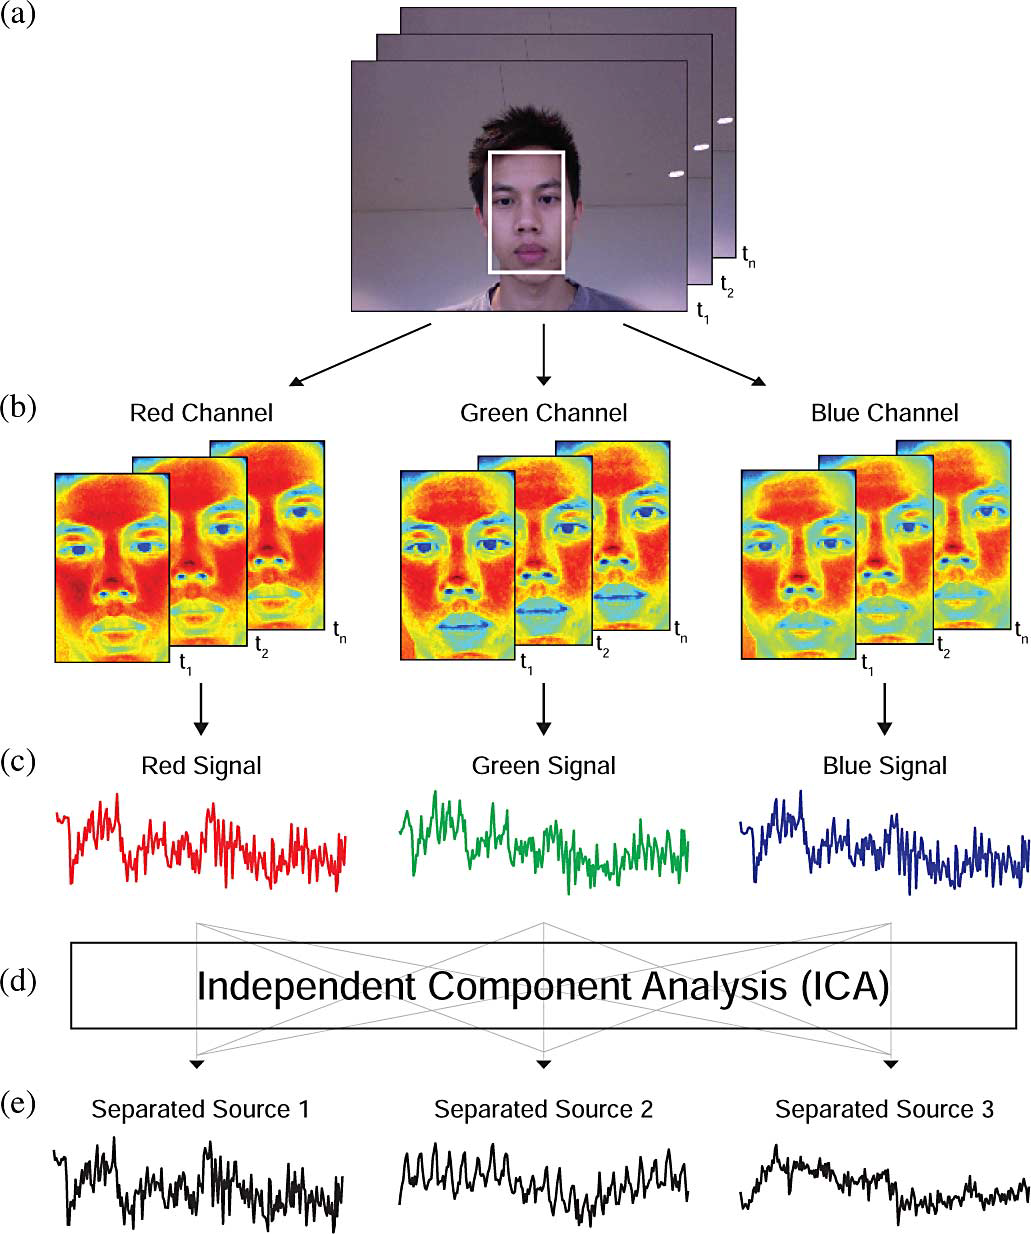
\includegraphics[width=0.7\linewidth]{Content/figures/poh.png}
\caption{rPPG approach based on ICA \parencite{poh2010non}.}
\label{fig:poh}
\end{figure}

\textcite{Datcu_2013} present a similar approach, however using AAM to segment the face of the subject into ROIs. \textcite{li2014remote} also use a different ROI, based on facial landmarks, and a combination of additional steps to mitigate noise caused by illumination, motion and facial expressions by removing signal outliers. \textcite{bousefsaf2013continuous} propose a variation of the previously described approaches, using a skin detection procedure to select pixels in the signal extraction phase. Additionally CWT is used in the signal estimation phase instead of the commonly used FFT, which is pointed by authors as more suitable for rapid changes in frequencies in time. As a consequence, the authors were able to detect the instantaneous HR (iHR) and significantly reduce the waiting time for the detection of HR measurements.

%used a digital version of the Stroop test and a video of a subject (captured by a webcam) to calculate HR and HRV to detect stress. A combination of HR, HRV and $HRV_{HF}$ is used to estimate the stress state. The resulting stress state curve tends to decrease during the rest period and increase during stress sessions (as the HR measurements), in accordance with previously mentioned works; additionally self-reported answers from questionnaires present significant differences of stress level in the rest and in the stress sessions as well, which confirms that remote reading and processing of HR as an input signal is able to relate with the real emotional state of an user. The detection mechanism, however, is purely based on the assumption that stress increases the HR mean. Both HR and HRV are averaged and interpolated within a time span (27 seconds) and the resulting wave produced from that calculation is said to be the stress level. Such wave might describe stress levels, since it matched variations of electrodermal response (EDR) data recorded using a skin conductance sensors, which is an indicator of stress, but the wave can also be seen as a simple representation of the HR and HRV variations, not stress itself.

Different approaches that are not based on the average of colors of the face can also be found in the literature. Those techniques use knowledge of the color vector of the different components to perform  the signal extraction. \textcite{Wang_2016novel} focus on the definition of a plane orthogonal to the skin-tone, ignoring pixels outside the subspace of skin pixels in the signal estimation phase. Similarly \textcite{de_Haan_2013} also use a skin model to generate a chrominance-based PPG signal, which is calculated as a combination of the intensities of the color channels in the video instead of their average. Those techniques aim to be more resilient than BSS-based techniques regarding motion noise. \textcite{6619284} are the first to completely move away from color-based initiatives and perform the signal extraction based on head movements. \textcite{Irani} further improved the technique by using a moving average filter applied to the trajectory of the feature points being tracked to remove the noise produced by other sources of motion, e.g. respiratory activity.
%Yun et al. \parencite{yun2009game}, on the other hand, demonstrated that changes in HR cause variation of temperature in the lower area of the forehead, which can be measured by a thermal imaging camera and used to infer stress state. The analysis performed by the authors was based on the variations of temperature in such lower area of the forehead, which differs from the color averaging approach previously described and used by other authors. The results, however, highlight that the region is affected by stress activities, which confirms the findings of \parencite{Datcu_2013}, \parencite{Sereevoravitgul} and \parencite{verkruysse2008remote} that point the forehead area as being more prone for remote readings.

The different settings in each phase of an rPPG technique result in a trade-off between advantages and disadvantages. Estimation based on head movement, e.g. \textcite{6619284}, does not rely on previous knowledge about colors nor requires visible skin area to work. However it is outperformed by other methods when subjects are not completely still \parencite{li2014remote} since it is significantly affected by subject motion. Techniques based on pre-defined skin-tone models, e.g. \textcite{Wang_2016novel,de_Haan_2013}, better adapt to changes in illumination (including non-white light sources), however they suffer performance degradation when the skin mask is not properly defined (or is noisy) or the pre-defined skin model is inaccurate \parencite{Wang_2016algorithmic}. Finally BSS-based methods, e.g. \textcite{poh2011advancements}, rely on BSS techniques (e.g. ICA) which are ideal to de-mix the estimated PPG signal from noise. However such techniques are unable to deal with periodic motion (i.e. exercise situation) and its statistical nature requires a long signal to enable an accurate measurement \parencite{Wang_2016algorithmic}. Despite such limitations, the ICA-based rPPG technique by \textcite{poh2011advancements} presents the best signal-noise ratio (SNR) for HR estimation under stationary situations (i.e. non-exercising) with different illumination conditions when compared to other techniques \parencite{Wang_2016novel}. The work is also extensively cited in the literature and often used as a benchmark for new techniques, which makes it a consolidated and robust solution.

%%%%%%%%%%%%%%%%%%%%%%%%%%%%%%%%%%%%%%%%%%%%%%%%%%%%%%%%%%%%%%%%%%%%%%%%%%%%%%%%%%%%%%%%%%%%%%%%%%%%%%%
\section{Accuracy and limitations}
%%%%%%%%%%%%%%%%%%%%%%%%%%%%%%%%%%%%%%%%%%%%%%%%%%%%%%%%%%%%%%%%%%%%%%%%%%%%%%%%%%%%%%%%%%%%%%%%%%%%%%%

The structure of rPPG techniques, as previously described, requires the analysis of each frame of a video to estimate the HR. As a consequence, any rPPG technique is influenced by the frame rate of the video, which accounts for the number of frames displayed per second (expressed in frames per second, or FPS), the resolution of each of those frames and the number of subsequent frames required to allow an estimation.

The frame rate of the video used in the estimation is directly connected to the sampling frequency, named $F_s$. Assuming that all frames of a video are used by an rPPG technique, a video running at 30 FPS allows a $F_s$ of 30 Hz, since each frames generates a sample. The minumum FPS required for the estimation must adhere to the Nyquist limit, which states that the sampling frequency must be at least twice as high as the highest frequency being measured:

\begin{equation*}
    F_s \geq 2 \cdot f_{Max}
\end{equation*}

where $f_{Max}$ denotes the highest frequency being measured. Since rPPG techniques are used to estimate HR, the value for $f_{Max}$ can be derived from a valid HR frequency interval. As previously described, a normal person presents a HR between the interval [45 bpm, 240 bpm], which is equivalent to the interval of [0.75 Hz, 4 Hz]. As a consequence, $f_{Max}$ is 4Hz (240 bpm) and $F_s$ is calculated as $F_s \geq 2 \cdot 4$, resulting in a minumum $F_s$ of 8 Hz, which translates to a video with frame rate of 8 FPS.

A fourier transform, e.g. FFT, is usually employed in rPPG techniques. The FFT divides the frequency spectrum of the input signal into $N$ number of discrete frequency blocks equal to the number of samples in the input signal. The number of samples $N$ used for the estimation is commonly refered to as window size. The smallest frequency that can be differentiated within that spectrum is named frequency resolusion, $\Delta f$, which is calculated as:

\begin{equation}
    \Delta f = \frac{F_s}{N}
    \label{eq:frequency-resolution}
\end{equation}

The frequency resolution $\Delta f$ influences the error rate in the estimation of the HR. For instance, if $\Delta f$ is 0.1 Hz, the HR will be estimated with an error of $\pm 3$ bpm. A low HR estimation error is desired, so a low value for $\Delta f$ is desired as well. By analysis of equation \ref{eq:frequency-resolution}, it is noted that $\Delta f$ descreases when $F_s$ descreases or when $N$ increases.

The value for $F_s$ is usually dependent on the camera device being used, which follows certain standards, e.g. 30 FPS. As a consequence, $\Delta f$ can be altered by changes on the window size $N$. Such changes, however, directly impact the estimations, since there is a trade-off between the window size and the estimation error. The higher the window size, the longer the video segment required for the estimation. Longer video segments are likely to contain movement of the subject being analyzed, which adds noise to the rPPG estimation.

\begin{table}[h!]
\caption{Frequency resolution $\Delta f$ (in Hz) as a function of window size (in samples) and frame rate (in FPS) \parencite{roald2013estimation}.}
\label{table:frequency-resolution}
\centering
\begin{tabular}{ccccccc}%
\toprule%
\textbf{Window size} & \textbf{10 FPS} & \textbf{15 FPS} & \textbf{25 FPS} & \textbf{30 FPS} & \textbf{50 FPS} & \textbf{60 FPS} \\
\midrule
100 & 0.1 & 0.15 & 0.25 & 0.3 & 0.5 & 0.6 \\
200 & 0.05 & 0.075 & 0.125 & 0.15 & 0.25 & 0.3 \\
300 & 0.033 & 0.05 & 0.083 & 0.1 & 0.17 & 0.2 \\
400 & 0.025 & 0.037 & 0.062 & 0.075 & 0.12 & 0.15 \\
500 & 0.02 & 0.03 & 0.05 & 0.06 & 0.1 & 0.12 \\
600 & 0.017 & 0.025 & 0.042 & 0.05 & 0.08 & 0.1 \\
700 & 0.014 & 0.02 & 0.03 & 0.04 & 0.07 & 0.08 \\
1000 & 0.01 & 0.015 & 0.025 & 0.03 & 0.05 & 0.06 \\
\bottomrule%
\end{tabular}%
\end{table}

\textcite{roald2013estimation} presents this trade-off by detailing the frequency resolution as a function of window size and video frame rate, as demonstrated in Table \ref{table:frequency-resolution}. As an example, assuming a video of 50 FPS and a frequency resolution of 0.07 Hz (which corresponds to an estimation error of $\pm 2.1$ bpm), a window size of 700 samples is required (equivalent of a video segment of 14 seconds). Additionally it has been proven that limitations in the sampling frequency, e.g. low $F_s$, can be compensated in the PPG signal detection by the use of interpolation \parencite{sun2012noncontact}.

\chapter{Multifactorial emotion estimation}
\label{ch:literature-multifactorial}

Previous chapters demonstrate the use of physiological signals and facial information applied separately to emotion estimation. The use of a single signal for the assessment is feasible, however a mapping process based on a multifactorial analysis, when more than one signal is used, is more likely to produce accurate results \parencite{kukolja2014comparative}. A combination of signals can reduce the interference/noise caused by signal manipulation.

Physiological signals, e.g. HR, are considered reliable sources since they are hard to fake (because of their link to the ANS), differently from facial expressions \parencite{Landowska}, for instance. When combined in the same analysis, however, those signals can complement each other and provide more information about emotional states.

The following sections present works related to multifacotiral emotion estimation categorized by contact (use of physical sensors) and non-contact (remote analysis) approaches.

\section{\sloppy Approaches based on physical contact and sensors}

The first multifactorial analysis approaches were based on obtrusive measurements of the input signals, where physical sensors were used. \textcite{Chanel_2011}, for instance, demonstrate the use of multifactorial input analysis to measure emotions and involvement in a game context. Participants play Tetris in different difficulty conditions while being monitored by a variety of sensors, which include a respiration belt and an electroencephalogram (EEG) system. The data from the EEG and the other peripheral signals are computed into two groups of features, which are used to train classifiers to recognize the states: boredom (low pleasure and low pressure, associated with easy difficulty), engagement (higher pleasure and motivation, associated with medium difficulty) and stress (anxiety and low pleasure, associated with hard difficulty). The classification accuracy of the model varies between 48\% and 55\% for different input signals, classifiers and feature selection.

\textcite{grundlehner2009design} also use physical sensors to perform real-time continuous arousal monitoring. The authors record and use four signals from subjects to estimate arousal: electrocardiogram (ECG), respiration, skin conductance and skin temperature. The ECG is used to calculate HRV, which is then used in the estimation. The data used for emotion-triggering is based on videos, sounds and a cognitive demanding game. A regression analysis is performed to identify the importance of the features in the estimation of arousal. $HRV_{LF}$ and $HRV_{HF}$ are not significant when compared to the other signals (e.g. skin conductance), while the standard deviation of HRV presents a significant weight. The arousal prediction matches the hypothesized arousal events marked by the authors in each of the emotion-triggering content. The results, however, were performed with controlled, pre-defined events that are expected to cause reactions, which might be related to arousal. More subtle or dynamic interactions, such as the ones obtained when a subject plays a digital game, might not be identified or detected by the approach proposed by the authors.

\textcite{bailenson2008real} use a combination of physiological signals (obtained from physical sensors) and facial expressions. The authors use a machine learning model to map the input signals to emotions (sadness or amusement). The training data used for the machine learning model is based on recordings of participants while they watched a video containing different emotion-triggering segments (neutral, amusement and sadness). Additionally 15 physiological signals are also used, among them HR, skin conductance level and finger temperature. The video recordings are annotated by professional coders. The annotated video frames are used in conjunction with the physiological signals to produce the predicting model. The authors compare the performance of models built from different data sources, such as the data from all subjects (general model), or from the female/male population (gender-specific model) or from a single individual (person-specific model). The model performs better when categorizing emotions instead of predicting its intensities and when detecting amusement instead of sadness. Additionally the person-specific model outperforms the other two variations, suggesting that a person-tailored model might be more effective in identifying features (even the more subtle ones) than a general-purpose model. The results also state that a model built from a combination of facial and physiological information is more efficient than a model built with either one alone.

\begin{figure}
\centering
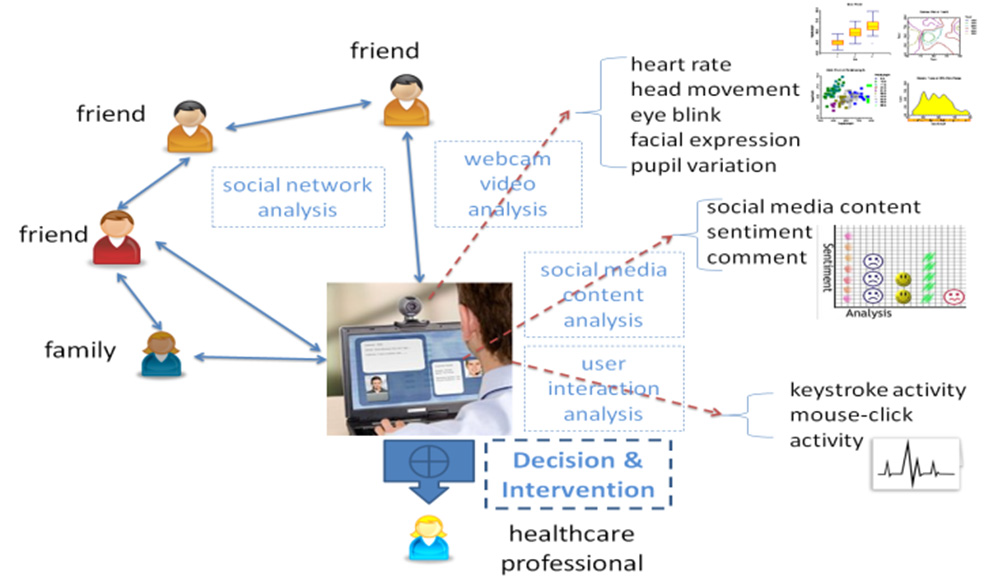
\includegraphics[width=0.9\linewidth]{Content/figures/zhou.png}
\caption{Non-obtrusive and remote approach based on multifactorial analysis to identify user emotion. Reproduced from \textcite{mental}.}
\label{fig:zhou}
\end{figure}

\section{\sloppy Approaches based on remote, non-contact analysis}

\textcite{mental} propose a completely non-obtrusive and remote approach based on multifactorial analysis to identify user emotion, as illustrated in Figure \ref{fig:zhou}. The main goal of such approach is aimed at monitoring patients mental health states. The model was created by weighting different features created from input signals, all obtained unobtrusively from a video of the subject's face and the textual content he/she created during the session (e.g. a reply to a tweet). The features are physiological (HR and pupil radius), physical (head movement rate, facial expression, eye blinking rate), based on human-computer interactions (mouse and keyboard usage rate) and based on sentiment analysis of social content (images and textual tweets). All features are used to train a multi-class classifier (based on logistic regression), which learns about the three possible emotion states: negative, neutral and positive. The emotion inference is performed in real-time and based on a probability rule: the state suggested by the classifier with the highest intensity is assumed to be the current subject's emotional state. The results show an accuracy rate of 89\% for negative, 56\% for neutral and 78\% for positive state identification. The authors do not specify, however, how much each input signals contributes to the emotional output. Additionally it is not possible to infer if such approach could be used outside the controlled environment created by the authors, which requires a simulation of a social network filled with previously defined and known content in order to work.

\textcite{mcduff2014remote} also use a camera to remotely measure cognitive stress via HRV. Participants are recorded while resting and while silently performing a mental arithmetic task. Facial landmarks are automatically detected and a ROI containing part of the subject's face is selected for analysis. Using a spacial average of the pixel intensities in each frame, a PPG signal is calculated through independent component analysis (ICA) and blood volume pulse (BVP) is extracted. Based on the discovered BVP, several other physiological parameters are calculated, such as HR, respiratory rate (RR), $HRV_{LF}$ and $HRV_{HF}$. The remote measurement of all physiological signals is in agreement with a physical device used as ground truth. Using those parameters, the authors construct a classifier, modeled with Naive Bayes and support vector machine (SVM), for predicting whether the subject is under cognitive stress. The input features used for the models are mean heart rate, mean respiratory rate, normalized $HRV_{LF}$ power, normalized $HRV_{HF}$ power and $HRV_{LF/HF}$ power ratio for each session. Results show that the prediction accuracy is 85\% using SVM, demonstrating that the input signals are sensitive enough to measure the cognitive stress state. The HRV components and the RR are the strongest predictors, while the is was not significantly different between the two detectable states. \textcite{mcduffcogcam} perform further investigations, however using different cognitive tasks (two cognitive demanding games). A person-independent machine learning model based on HR, HRV, $HRV_{LF}$, $HRV_{HF}$ (along with normalized and combined versions of those signals) and breathing rate is used to classify the stress level of the subjects. According to the authors, the average heart rate and breathing rate are not significantly different in any case, which differs from previous findings of other authors. The variations of $HRV_{LF}$ and $HRV_{HF}$, however, are significantly different during the cognitive tasks compared to the rest period; higher $HRV_{LF}$ and lower $HRV_{HF}$ power are found in both cognitive tasks compared to the rest period, which aligns with findings of previous work. Authors also point out that the stress predictions made by the model are consistent with the self-reported answers. The two participants with the highest self-reported stress level show the highest predicted stress level, while the two participants with the lowest self-reported stress level also present the lowest predictions. %It emphasizes the challenges associated with the great variability between individuals regarding physiological signals and emotional state, such as stress.

\begin{figure}[h]
    \centering
    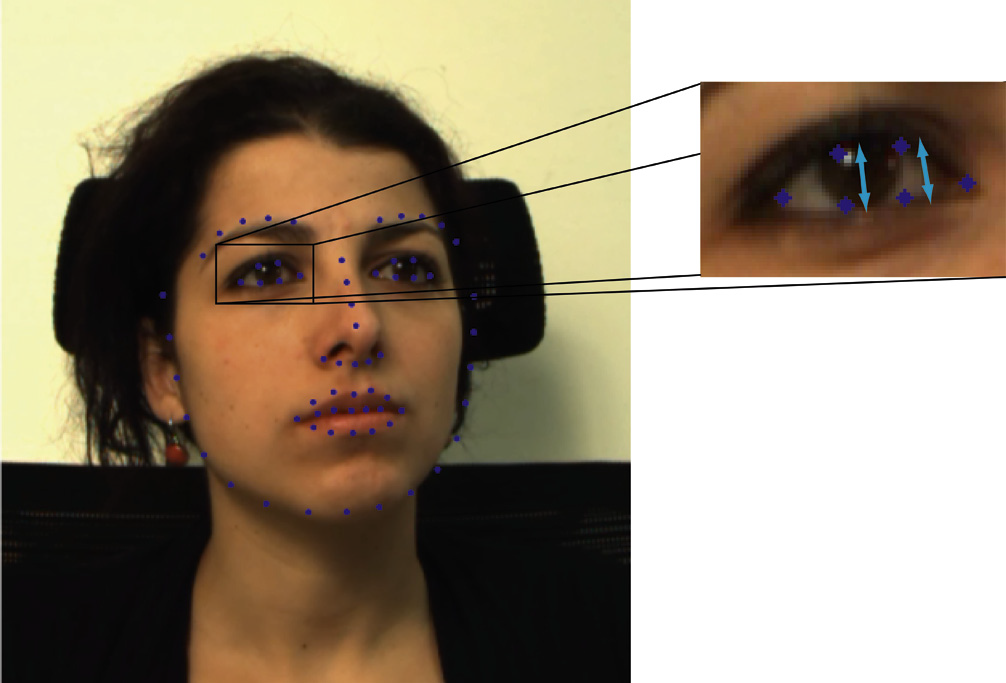
\includegraphics[width=0.7\linewidth]{Content/figures/giannakakis2017stress-eye.png}
    \caption{Highlight of distance calculation regarding eye aperture. Reproduced from \textcite{giannakakis2017stress}.}
    \label{fig:giannakakis2017stress-eye}
\end{figure}

Finally \textcite{giannakakis2017stress} present an approach for detection of stress/anxiety based on eye blink, mouth/head movements and HR estimations using rPPG. Participants are recorded while performing a set of tasks designed to trigger emotional responses, such as talking in a foreign language, remembering a sad incident, visualizing images/videos and playing a gamified cognitive test, i.e. Stroop test. Facial cues are obtained from an automatically detected ROI. Those cues are used to extract facial features, which are related to eyes, mouth, and head movement. Figure \ref{fig:giannakakis2017stress-eye} highlights the facial analysis used in the calculation of eye apperture, which is one of the features extracted and used in the emotion detection. The extracted features, including HR information estimated using rPPG, are selected and ranked accordinly to maximize a machine learning classification step. Different classifiers are employed, which yield different classification accuracy rates. For each task performed by the subjects, classification accuracy ranges between 80\% and 90\% taking into account the most efficient classifier. It is noted by the authors that the observation of stressful images and the interaction with the Stroop test appear to be the most consistent across the classifiers employed.


\part{Experiments}
\chapter{Experiment 1: provoked stress and boredom}
\label{ch:experiment1}

The experiment described in this chapter, the first one conducted, aimed at gathering data and exploring the relations regarding facial actions (FA), HR and emotional states, particularly stress and boredom. The experiment is based on the previously mentioned findings that HR varies according to stress/frustration and that facial expressions can convey contextual information about emotional state \parencite{giannakakis2017stress}. As opposed to previously mentioned works, in this experiment each subject spends an average of 25 minutes in the session, playing three different games that were custom-made to provoke the emotional reactions similar to off-the-shelf games. Subjects were also not instructed regarding how they should move, so body and facial reactions are likely to be the ones the subject would normally perform under a gaming context. The approach consists of using induced boring to stressful mechanics in the games to produce variations in the emotional state and HR of participants. %, based on the previously mentioned findings that HR varies according to stress/frustrations.

%FA were manually detected and annotated based on observations.
In total, three studies were performed on the data obtained from the experiment. The first study focuses on empirical exploration of how FA, defined as being any facial movement different from a neutral face, e.g. lips contraction, relate to emotional states. The second study focuses on the variations of HR that occurred during the interaction with the games, specially under situations that were designed to provoke boredom and stress. It should confirm the hypothesis that the HR during boring and stressful parts of a game is in fact different. Finally the third study focuses on the accuracy evaluation of an rPPG technique when applied to gaming sessions where subjects behave naturally.

The following sections present information regarding the participants, the experiment structure and each one of the mentioned studies.

%. Our experiment allows the investigation of variations of HR and FA in a context where boredom and stress were induced on purpose. As a result of our experiment, we present information regarding the changes in the HR mean of subjects while they play games that are deliberately boring and stressful; additionally we present a set of annotated FA that happened during the phases of the games that were perceived as being boring and stressful.

%The remote detection of HR proved a promising approach to infer boredom/stress levels \parencite{kukolja2014comparative} or cognitive stress \parencite{mcduff2014remote} of a person. Experiments regarding such approaches, however, were performed under extremely controlled situations with few game-related stimuli. A significant limitation of such approaches was that subjects were asked to remain still during the experiment. Another problem is that subjects had limited interaction with the content being presented: they performed tasks mentally (e.g. counting), watched videos/images or performed gamified cognitive tests for a short period of time. Those are artificial situations that are unlikely to happen in real-life situations, especially in a gaming session with a challenging game lasting for several minutes. In that situation, the subject will probably move and present variations of facial actions during the gaming session \parencite{bevilacqua2016variations}.

%%%%

\section{Participants}

Twenty adult participants of both genders (10 female) with different ages (22 to 59, mean 35.4, SD 10.79) and different gaming experience gave their informed and written consent to participate in the experiment. The study population consisted of staff members and students of the University of Sk\"ovde, as well as citizens of the community/city. When asked how skilled subjects believe they are at playing video games, 1 subject (5\%) reported no skill, 10 (50\%) reported not very skilled, 7 (35\%) reported moderately skilled and 2 (10\%) reported very skilled. When asked the number of hours per week they had played any type of video game over the last year, 2 subjects (10\%) reported more than 10, 6 (30\%) reported 5 to 10, 2 (10\%) reported 3 to 4, 2 (10\%) reported 1 to 3, 4 (20\%) reported 0 to 1, and 4 (20\%) reported no activity. Those numbers indicate that the population has a diversity of gaming experience and playing frequency, which provides the experiment with information that is less skewed towards specific profile of players, e.g. hardcore players.

\section{Materials and procedures}

Subjects were seated in front a computer, alone in the room, while being recorded by a camera and measured by a heart rate sensor. The camera was attached to a tripod placed in front of the subjects at approximately 0.6m of distance; the camera was slightly tilted up. A spotlight, tilted 45$^{\circ}$ up, placed at a distance of 1.6m from the subject and 45cm higher than the camera level, was used for illumination; no other light source was active during the experiment. Figure \ref{fig:setup} illustrates the setup.

\begin{figure}[h]
\centering
\includegraphics[width=\textwidth]{Content/figures/experiment-setup-double}
\caption{Experiment setup. On the left, illustration regarding the position of equipment, including the angle of the external light source. On the right, highlight of the position and angle of the video camera.}
\label{fig:setup}
\end{figure}

The participants were each recorded for about 25 minutes, during which they played three games. Each game was followed by a questionnaire related to the game and stress/boredom. The first two games were followed by a 138 seconds rest period, where the subjects listened to calm classic music. The last game was followed by an additional questionnaire about age and gaming experience/profile. The order which the games were played was randomized among subjects. Participants received instructions from a researcher that they should play three games, answer a questionnaire after each game and rest; they were told that their gaming performance was not being analyzed, that they should not give up in the middle of the games and that they should remain seated during the whole process.

After each game, subjects answered a questionnaire in order to provide self-reported stress and bordeom measurements. The questionnaire had six questions: the first four were a 5-point Likert scale related to how the player felt related to stress/boredom at the beginning/end of each game (1: not stressed/bored at all, 5: extremely stressed/bored); a question to identify the part of the game that best describes the moment the subject enjoyed the most (very beginning, after beginning and before middle, middle, after middle and before end, very end); finally a question asking if the subject understood the game. Before the end of the experiment, subjects answered a final questionnaire with nine questions, which were related to: age; gender; number of hours per week spent with games over the last year (question from the video game experience questionnaire \parencite{unsworth2015playing}); how proficient or skilled the subject believe being at playing video games (question from the Survey of Spatial Representation and Activities - SSRA \parencite{terlecki2005important}); familiarity with puzzle, platform and Tetris games; current state of mind compared to other days (e.g. normal, unusually stressed, etc.); and gaming profile (like, dislike challenging games).

Regarding the self-reported levels of stress and boredom provided by subjects after each game, the answers were given according to the participant's own interpretation of such levels. As a consequence we are not able to treat the answers as a uniform scale with a defined degree of difference among values. Because of that we decided to use a Wilcoxon Signed-rank test to statistically check if the reported boredom levels at the end are significantly different from the ones at the beginning of the games, as well as if the reported stress levels at the end are different from the ones at the beginning of the games. For the Mushroom game, the reported boredom levels at the beginning (median 3.5) were significantly higher than the reported levels at the end (median 1) of the game, $Z=-2.69$, $p<0.01$. Regarding the reported stress levels, values at the beginning (median 1) were significantly lower than the reported levels at the end (median 3), $Z=3.63$, $p<0.01$. For the Platformer game, boredom levels at the beginning (median 3) were higher than the ones at the end (median 1), $Z=-2.47$, $p<0.05$. Regarding stress levels, values at the beginning (median 1) were lower than the ones at the end (median 4), $Z=3.79$, $p<0.01$. Finally for the Tetris game, boredom levels at the beginning (median 4) were higher than the ones at the end (median 2), $Z=-2.97$, $p<0.01$. Regarding stress levels, values at the beginning (median 1) were lower than the ones at the end (median 4), $Z=3.95$, $p<0.01$.

The self-reported answers support the idea that subjects perceived the three games as being boring at the begin and stressful at the end, which was the intended result of our design process.

\section{Data collection}

During the whole experiment, subjects were recorded using a Canon Legria HF R606 video camera. All videos were recorded in color (24-bit RGB with three channels $\times$ 8bits/channel) at 50p frames per second (fps) with pixel resolution of 1920 $\times$ 1080 and saved in AVCHD-HD format, MPEG-4 AVC as the codec. At the same time, subject's HR was measured by a TomTom Runner Cardio watch (TomTom International BV, Amsterdam, Netherlands), which was used as ground truth. The watch was placed on the left arm, approximately 7cm away from the wrist, like a regular wrist watch, and its use was unobtrusive, so it did not affect the movements of the subjects, who could still use both hands to play the games. The watch recorded the HR at 1 Hz.

\section{Games and stimuli elicitation}
\label{sec:experiment1-games-elicitation}

The three games\footnote{Source code available at: https://fernandobevilacqua.com/link/phd-experiment1} used in the experiment were 2D and casual-themed, played with mouse or keyboard in a web browser. The games were carefully designed to provoke boredom at the beginning and stress at the end, with a linear progression between the two states (adjustments of such progression are performed every 1 minute). The game mechanics were chosen based on the capacity to fulfill such linear progression, along with the quality of not allowing the player to instantly kill the main character (by mistake or not), e.g. by falling into a hole. The mechanics were also designed/selected to ensure that all subjects would have the same game pace, e.g. a player must not be able to deliberately control the game speed based on his/her will or skill level.

The \textbf{Mushroom} game, illustrated in Figure \ref{fig:mushroom-platformer-tetris} (left), is a puzzle where the player must feed a character by dragging and dropping mushrooms in rounds. In a given round, $M$ mushrooms are displayed in a grid and the player has $K$ seconds (a decreasing time bar at the top informs the remaining time) to collect good and discard bad (poisonous) mushrooms. At the upper-right corner of the screen, a sign informs the player about the bad/poisonous mushroom of the round. The player must drag and drop all good mushrooms (the ones different from the poisonous indication) into the character, while dragging and dropping the bad ones into the trash can. Mushrooms are differentiated by the colors of their features (circles). The player is rewarded with score points, a health bar increase ($HB\textsubscript{I}$) and a pleasant sound when a right move is performed. In case of mistake a health bar decrease ($HB\textsubscript{D}$) and an annoying/aggressive alarm sound is applied. If the time $K$ is over and the player has not finished moving all the mushroom of the round, each remaining mushroom in the grid is counted as a mistake. If the grid is clean and there is still time available, the player must wait until the time is over. The values of $M$, $K$, $HB\textsubscript{I}$ and $HB\textsubscript{D}$ are used to induce boredom/stress. At the beginning, $M$ is low (starts with 2) and $K$ is high (starts with 45 seconds), so the player spends a significant amount of time waiting for the game to continue; every 1 minute the value of $M$ is increased and $K$ is decreased. The changes continue to happen until the player is unable to deal with the amount of mushrooms within the available time. This leads to mistakes that will eventually decrease the health bar to zero, terminating the game. After the mark of 6 minutes, the game becomes virtually impossible to beat.

The \textbf{Platformer}, illustrated in Figure \ref{fig:mushroom-platformer-tetris} (center), is a side-scrolling, endless runner game where the player must control the main character while collecting hearts and avoiding obstacles (skulls with spikes). The character can jump (by pressing the up arrow key in the keyboard) or slash (S key), however the player is not able to move the main character left or right, it remains in the same position on the screen (towards the left side of the screen). The character moves on top of platforms, which are always perfectly connected, so there are no gaps (holes) among them; the height of the platform can vary, however, so there might be a slope up/down connecting two platforms, for instance. If the character hits an obstacle, the health bar is decreased ($HB\textsubscript{D}$) and a sound effect related to pain is played. If any heart is collected, the health bar increases ($HB\textsubscript{I}$) and a pleasant sound effect is played. The position where the hearts appear on each platform is adjustable (defined by $HH$), so they can appear close to the platform (no action is required to collect the heart) or a bit higher from the ground (jump action is required to collect the heart). The speed of the character ($S$, which is the velocity at which elements are moving on the screen), the height variation of each new platform that appears on the screen ($HV$), the amount of hearts ($G$) and obstacles ($E$) per platform are all controlled by the game and used to adjust boredom/stress. At the beginning, boredom is induced by keeping all previously mentioned parameters with low values, which means the game is slow, the character moves from platform to platform at the same height and almost no hearts or obstacles appear on the screen. The few hearts that are available are placed close to the ground to destimulate jumping actions. As time progresses, the values of $S$, $E$, $HV$, $HB\textsubscript{D}$ and $HH$ increase, while $G$ and $HB\textsubscript{I}$ decrease to induce the player to a stressfull state. At the mark of 5 minutes, for instance, the game is significantly fast, with several obstacles on the screen and almost no hearts to collect; the damage caused to the character when hit by an obstacle is also higher than the beginning of the game. The linear increase in difficulty will eventually result in consecutive hits (mistakes), which will decrease the health points until zero, when the game ends.

\begin{figure*}[!h]
\centering
\includegraphics[width=\textwidth]{Content/figures/experiment1-games}
\caption{Mushroom (left), Platformer (center) and Tetris (right). In Mushroom, player has to drag and drop the correct mushrooms into the character, discarding the wrong ones into the trash. In Platformer, the player has to jump over or slide under obstacles while collecting hearts. In our version of Tetris, there are no hints about the next piece to be added to the screen}
\label{fig:mushroom-platformer-tetris}
\end{figure*}

Finally the game \textbf{Tetris}, shown in Figure \ref{fig:mushroom-platformer-tetris} (right), is a modification of the original Tetris game. In our version of the game, the next block to be added to the screen is not displayed, so the player is unable to predict future moves. Additionally, the down key, usually used to speed up the descendant trajectory of the current piece, is disabled. The keyboard controls are the arrow keys to move the piece left/right and the R key to rotate the piece. The game is also modified to ensure that all subjects received the same sequence of pieces (we use the same seed for the generation of random numbers). The speed that the pieces fall ($S$) is used to control boredom and stress; at the beginning of the game, boredom is induced by using a low value for $S$, which makes the game slow since the pieces are falling slowly and the player is unable to speed them up. As time progresses, $S$ increases linearly making the game faster and harder to play, which should induce stress. At the mark of 5 minutes, for instance, a single piece takes almost 1 second to traverse the whole screen.

\section{Study 1: variations of facial actions}
\label{sec:experiment1-study1}

This study presents information regarding FA that the subjects presented during the experiment. The 6 hours of recordings of all subjects were manually analyzed and FA were annotated empirically. The annotations were categorized according to the period when they happened (the boring first part or the stressful second part of the games). An analysis on such annotated FA was conducted on group and individual level, aiming to find patterns between the featured FA and the boring/stressful periods of the games.

The following sections presents the analysis, discussion and results of the gathered information.

\subsection{Analysis and methods}
\label{s:experiment1-study1-methodology}

The recordings of all subjects were analyzed by a single reseacher who took notes of any facial actions (FA) that were different from a neutral (resting) face, e.g. lips contraction, brow movement, etc. Annotations were not performed periodically, e.g. every 5 seconds, instead they were made only when the subject's face changed from its neutral/resting state. As a consequence, if the subject remained with a neutral face for a long period of time, no annotations were made during that period.

The use of such empirical and non-standard approach for facial annotation was used because focus is not on facial expressions \textit{per se}, but in the exploration of any facial action (standardized or not) that might be used to infer patterns in boredom/stressful states. This approach is not without its limitations, however it provides a reasonable empirical perception of facial activity that is different from a neutral face, which is satisfactory for the investigation. FA are subtle and not necessarily part of a complete facial expression, e.g. surprise face, so they might be better identified in a context where annotations are made only when facial changes happen, as opposed to a frame-by-frame analysis/annotation of a video, for instance.

\begin{figure}[!h]
\centering
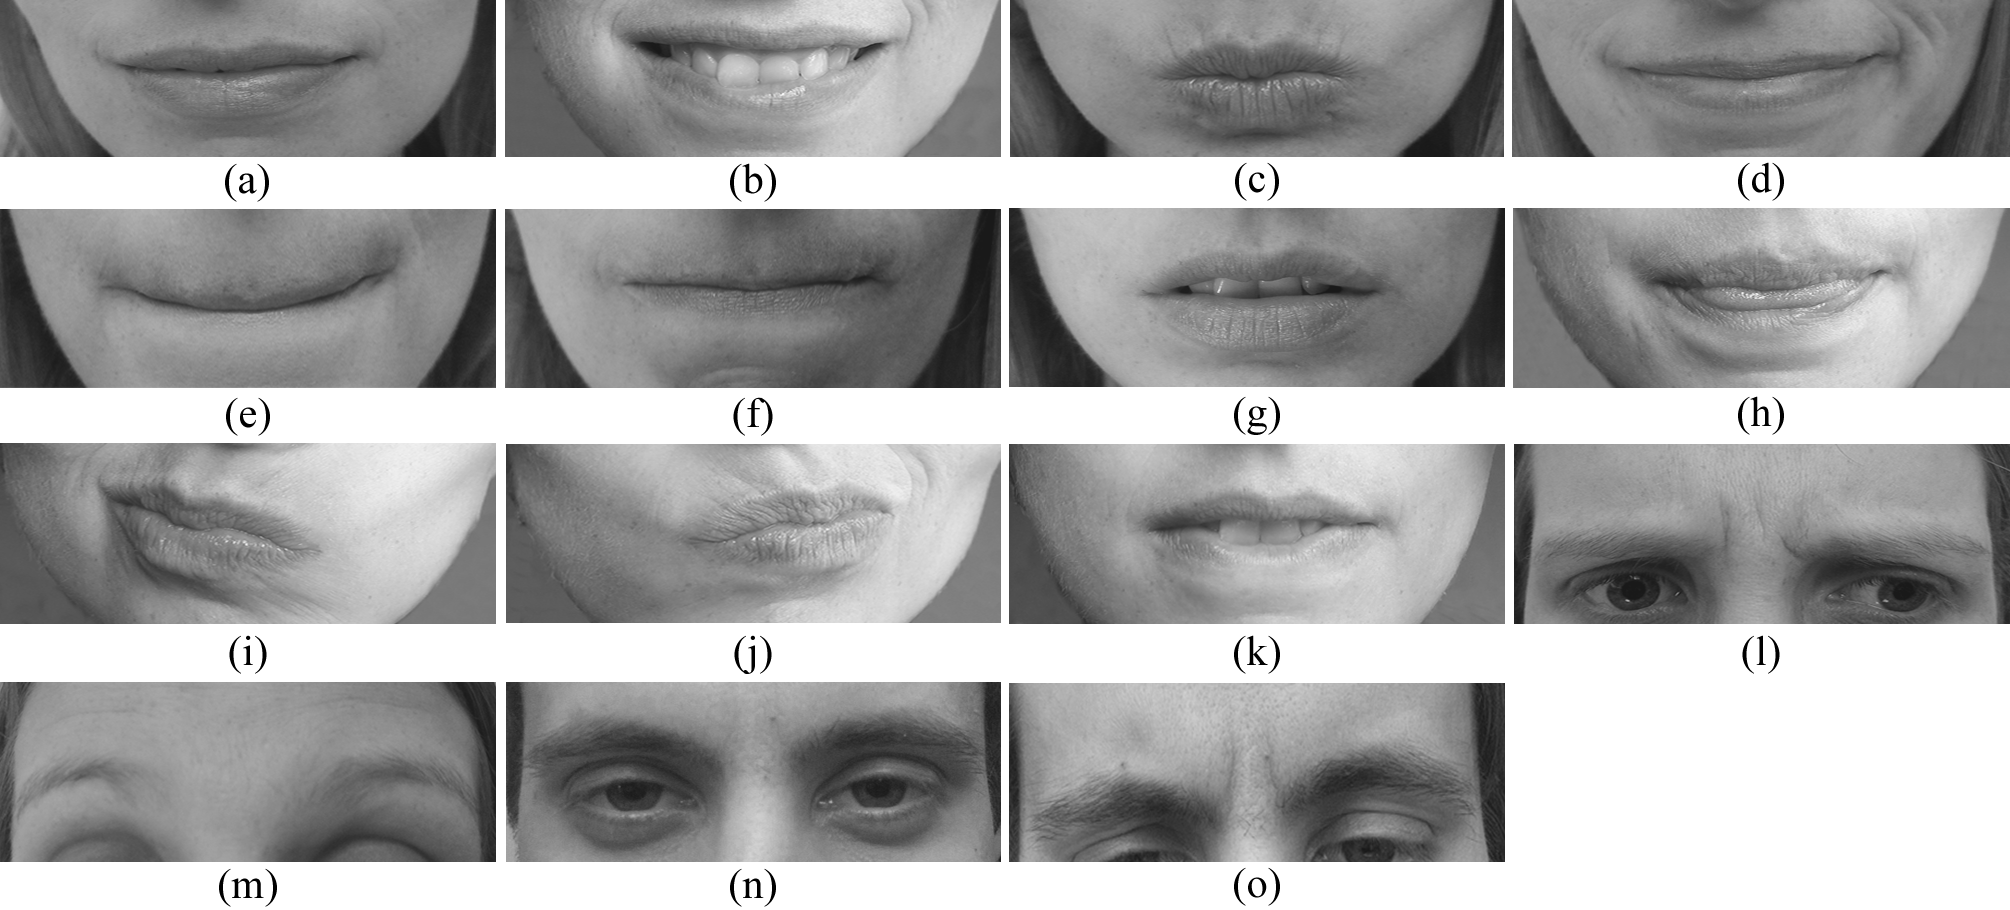
\includegraphics[width=0.4\textwidth]{Content/figures/facial-actions}
\caption{Annotated facial actions (FA). (a) Smile not showing teeth; (b) Smile showing teeth; (c) Lip puckerer; (d) Lip stretcher; (e) Lip suck; (f) Lip pressor; (g) Lips parted; (h) Tongue touching lips; (i) Mouth movement right; (j) Mouth movement left; (k) Lower lip bite; (l) Frown; (m) Brow raiser; (n) Lid tightener; (o) Brow lowering}
\label{fig:fa}
\end{figure}

According to the design of the games, subjects are supposed to perceive the experience during the beginning of the games as being more boring than the one at the end, while the experience at the end should be perceived as more stressing than the one at the beginning of the games. As a result, if the game sessions of each subject is divided in half, in theory one of the two resulting parts is more likely to be perceived as more boring by the subjects, while the other is more likely to be perceived as more stressful. Using that assumption, FA annotations were divided in two groups, the ones made during the period that corresponds to the first half ($H_0$) of the games and the ones made in the second half ($H_1$). Such division of the annotation aimed to identify any pattern regarding FA happening during periods theoretically perceived as boring or stressful. After all annotations were made, an identification of uniqueness was performed and, based on that information, the repetitions of such unique actions across the games for all subjects was counted. As a result, the frequency that each FA appeared during all game sessions was obtained, as well as when they happened (in $H_0$ or $H_1$). Any FA that appeared just a single time during the whole 6 hours recording was excluded from the list, assuming that such action was noise or probably part of another action. As a result 17 unique FA that appeared in the recordings at least twice were identified. Excluding the talking and laughing FA, Figure \ref{fig:fa} illustrates all annotated FA. Finally after all annotations were counted and categorized according to the period in the game, a per-subject evaluation regarding the frequency of FA was conducted. For each subject, an inspection was performed regarding FA that appeared in $H_1$ of all three games with a higher frequency than in $H_0$, and vice versa (appeared in $H_0$ of all three games with a higher frequency than in $H_1$).

\subsection{Results}

\begin{table}[h!]
\caption{Amount of FA annotations made for all subjects during periods $H_0$ and $H_1$ of the games}
\label{table:amount-fa}
\centering
\begin{tabular}{L{.4\linewidth}C{.2\linewidth}C{.2\linewidth}}%
\toprule%
\textbf{Game} & \textbf{Period $H_0$} & \textbf{Period $H_1$} \\
\midrule
Mushroom   & 90 & 98 \\
\midrule
Platformer & 88 & 181 \\
\midrule
Tetris     & 110 & 159 \\
\bottomrule%
\end{tabular}%
\end{table}

The number of subjects that featured a particular FA was analized, alongside with the number of repetitions of such FA, for all three games. The analysis is also divided according to the period of the game. Only FA featured by two or more subjects were considered, since it produces an analysis that is connected to more frequent FA among the whole group of subjects instead of the peculiarities of a single person. Table \ref{table:amount-fa} shows the amount of FA annotations made for all subjects during the games. According to the results, the amount of FA annotations made during $H_1$ (second half) of all three games was greater than the amount of annotations made during $H_0$ (first half). The increase in annotations during $H_1$ compared to $H_0$ was 8.8\%, 105.6\% and 44.5\% higher for the Mushroom, Platformer and the Tetris game, respectively.

Regarding the FA annotated during each game, for the Mushroom game, the three most frequent FA in $H_0$ were frown (repeated 16 times among 5 subjects), talking (12 times, 3 subjects) and tongue touching lips (9 times, 3 subjects). The three most frequent FA in $H_1$ were frown (repeated 16 times among 3 subjects), talking (13 times, 5 subjects) and lips parted (13 times, 5 subjects). By comparing most frequent FA in the two periods, both frown and talking are present, however they were not featured by a significant number of participants. In fact no more than 5 subjects (25\% of the participants) featured one of those FA. It suggests that individuals present distinct facial behaviors that are not easily generalizable, even in the same context. Curiously, two particular FA presented a significant change in the amount of repetitions and subjects between the two periods: lip pressors (from 7 to 11 repetitions, 2 to 4 subjects) and lips parted (from 5 to 13 repetitions, 2 to 5 subjects). When compared to the whole group of participants, such increase is not significant (again they represent less than 25\% of the participants), but it might be the indication of a pattern for two or three subjects. As suggested by previous work, the combination of such particular changes with another physiological signal, e.g. HR, might produce an acceptable detector for boredom/stress emotional state.

For the Platformer game, the three most frequent FA for $H_0$ were frown (19 repetitions among 3 subjects), tongue touching lips (12 repetitions, 3 subjects) and smile not showing teeth (11 repetitions, 3 subjects). For $H_1$, the FA were frown (49 repetitions, 5 subjects), smile not showing teeth (21 repetitions, 7 subjects) and lips parted (17 repetitions, 5 subjects). By comparing the FA in both periods, frown was featured by more subjects (5, representing 25\%) during the stressful part of the game, however more participants (7, representing 35\%) also featured smiles not showing teeth as well. Additionally to those FA, 25\% of the participants featured talking behavior during $H_1$, externalizing game decisions.

For the Tetris game, the three most frequent FA for $H_0$ were frown (36 repetitions among 4 subjects), smile not showing teeth (14 repetitions, 4 subjects) and lip pressor (11 repetitions, 4 subjects). For $H_1$, the FA were frown (42 repetitions among 4 subjects), lip pressor (28 repetitions, 6 subjects) and smile not showing teeth (16 repetitions, 5 subjects). By comparing those results to the most frequent FA in the Mushroom game, only frown is present in both; it is important to stress that frown was featured by less than 25\% of the participants in both games, which highlights the difficulties in finding a pattern that can be applied to all subjects to identify a boring or a stressful situation, even when the most frequent FA are used. On the other hand, two FA presented a significant change from one period to another in the Tetris game: lip pressor (from 11 to 28 repetitions, 4 to 6 subjects) and talking (from 0 to 15 repetitions, 0 to 6 subjects). Both actions were featured by 30\% of the participants, which could be further investigated in the pursue of FA that can help in the identification of emotional states. Regarding the talking FA, it has been observed from the recordings that some subjects tended to externalize in words any wrong decisions they made in the game, such as how pieces were positioned, in a similar way observed during the Platformer game; in that sense, talking could be used as an indicator of activity in the game, since it is a clear facial manifestation that happened, in this case, when players were frustrated. For further FA analysis based on a group level, see \parencite{bevilacqua2016variations}.

Finally a per-subject inspection of all annotated FA was conducted according to the procedure described in Section \ref{s:experiment1-study1-methodology}. The aim was to identify, for each subjects, which FA appeared in $H_0$ (or $H_1$) of \emph{all} three games with a higher frequency than they did in $H_1$ (or $H_0$), if any. Table \ref{table:individual} shows the results of such inspection. Marked numbers represent the frequency of a FA that was present in all three games for the specified subject and period. In total 10 participants (50\%) featured at least one FA that appeared in all three games, in the same period (boring or stressful part) with a frequency equal or greater than its appearance in the counter-period. Subject 2, for instance, featured one lip pressor during $H_0$, while the total number of times the same FA appeared in $H_1$ for all three games combined was 18. It is important to highlight that subject 16 was the only one who featured a FA more frequently in $H_0$ of all three games than he/she did during $H_1$; all other subjects featured FA more frequently in $H_1$ than in $H_0$.

\begin{table}[!h]
\caption{Subject-based frequency of FA that appeared in the same period of all three games}
\label{table:individual}
\centering
\begin{threeparttable}
\begin{tabular}{cp{.4\linewidth}cc}
\toprule%
\textbf{Subject} & \textbf{FA} & \textbf{Period $H_0$} & \textbf{Period $H_1$} \\
\toprule%
2 & Lip pressor & 1 & 18\tnote{b} \\
\midrule
15 & Lip pressor & 2 & 9\tnote{b} \\
\midrule
10 & Laughing & 2 & 19\tnote{b} \\
\midrule
14 & Laughing & 3 & 9\tnote{b} \\
\midrule
12 & Smile not showing teeth & 2 & 8\tnote{b} \\
\midrule
13 & Smile not showing teeth & 0 & 6\tnote{b} \\
\midrule
18 & Smile not showing teeth & 4 & 10\tnote{b} \\
\midrule
11 & Lips parted & 1 & 10\tnote{b} \\
\midrule
17 & Lip stretcher & 0 & 8\tnote{b} \\
\midrule
16 & Talking & 7\tnote{b} & 1 \\
\bottomrule
\end{tabular}
\begin{tablenotes}
\small
\item[b]{FA was present in all three games for the specified subject and period.}
\end{tablenotes}
\end{threeparttable}
\end{table}

\subsection{Discussion}

About the FA, even though further investigation is required, calculations indicate that subjects featured a neutral face for a longer period of time during the first half ($H_0$) of all games when compared to the second half ($H_1$). Since FA annotations were made only when the subject's face featured anything different from her/his neutral face, more annotations indicate more facial activity. Additionally the results might indicate that subjects featured more FA (different from the neutral face) under stressful situations than they did under boring situations, where a neutral face/expression is probably dominant.

The games used in the experiment were designed to gradually increase the difficulty level until the subject was not able to handle it. As a consequence, it is possible to postulate that smiles and laughs during the second half could be connected to the subject's perception that the games were too difficult to continue playing properly. On the other hand, they could indicate genuine manifestations of enjoyment during the moments the subjects felt the game was properly balanced and engaging. Regarding the other FA, such as lip pressor and lips parted, further investigation is required to accurately connect or use such actions to predict/detect emotional states, however the results show a clue about how FA variations can be different on the individual level. As previously discussed, the analysis and generalization of FA on a group level is less clear than an individual approach, since FA behavior might be specific to each person. The per-subject analysis indicated that, for a portion of the participants, at least one FA was present in the three games, in the same period for the same person. Such information might be used as the starting point for further investigation regarding FA and an individual-tailored detection model for boredom/stress, for instance.

%%%%%%%%%%%%%%%%%%%%%%%%%%%%%%%%%%%%%%%%%%%%%%%%%%%%%%%%%%%%%%%%%%%%%%%%%%%%%%%%%%%%%
%\subsection{Limitations}
%%%%%%%%%%%%%%%%%%%%%%%%%%%%%%%%%%%%%%%%%%%%%%%%%%%%%%%%%%%%%%%%%%%%%%%%%%%%%%%%%%%%%

%One potential limitation of our work is the internal validity. As previously described, the experiment was based on a one-group posttest design, which does not use a control group to measure the effects of the treatment. Such design could be criticized for having low internal validity, since it is not possible to unambiguously attribute cause and effect \parencite{kirk1982experimental}. A two-group approach could be suggested as having stronger internal validity, since it contains a control group and allows a less ambiguous conclusion. In the context of our research, however, any multiple group design implies the comparison of physiological signals and emotional perceptions among different people. Given the social and cultural background of the participants, it is virtually impossible to compare two groups of people regarding stress/boredom. People have different preferences, culture and expectations, which cause maturation and history threats to internal validity \parencite{trochim2001research}. Additionally the process of comparing variations of physiological signals among different subjects is a complex task, even when subjects are similar, e.g. same age and sex. As a consequence, a subject in a control group might present a set of variations of signals and classify a game as boring, while a similar subject in another group might classify the same game as not boring at all, presenting a different set of variations of signals. In that light, our experiment relies on a one-group experimental design to increase internal validity, since subjects were compared with themselves, which removes inter-subject differences.

%Another limitation is the empirical approach used to annotate the FA, which was not based on a formal scheme and was conducted by a single person without validation by other researchers. We believe that the exploratory nature of our study regarding FA allows the use of such approach. Our aim was not to standardize FA regarding stress/boredom, but to document the perceptions of naked-eye observations of FA in a context involving games, so that it can be used to guide further steps regarding the utilization of FA in a multifactorial analysis. A frame-by-frame annotation of our video recordings using a formal scheme, such as FACS, would be a significantly laborious and time-consuming task, which is not motivated by our exploratory and empirical approach. Another limitation is the assumption used when dividing each game session in half, presuming that the middle point of the period indicates a transition from two distinct periods: $H_0$, perceived as more boring, and $H_1$, perceived as more stressing. It is not necessarily true. Even though our data indicate that subjects perceived the beginning of the games as being boring and the end as being stressful, our point of division or the periods themselves remain an assumption. There might be moments towards the end of the game, for instance, that could be perceived as more boring or joyful depending on the subject, since each participant has her/his own specific expectations and skill level regarding games. Finally the core mechanic of the Mushroom game is based on the color of the mushrooms (instead of patterns, for instance), which is not suitable for color blind subjects.

\subsection{Conclusion}

%This paper presented the description and results of an experiment aimed at exploring the variations of heart rate (HR) and facial actions (FA) during gaming sessions with induced boredom and stress. In total twenty adults of different ages and gaming experiences participated in the experiment, where they played three different games while being recorded by a video camera and monitored by a HR sensor. The games used in the experiment were carefully designed and implemented to have a difficulty level that linearly increases over time, from a boring to a stressful point. According to self-reported answers in post-games questionnaires, participants perceived the games as being boring at the beginning and stressful at the end. Such configuration gives our experiment a novel approach for the exploration of HR and FA regarding their connection to emotional states, since information can be categorized according to the induced (and theoretically known) emotional states.

Results show that more FA annotations were made during the stressful part of the games, which indicates that participants remained with a neutral face for longer periods of time during the boring part. The analysis on group level revealed that any FA pattern was related to 5 subjects (25\% of the group) at most. In the analysis conducted on the individual level, particular patterns were found for 10 subjects (50\% of the group).

%Our findings suggest that changes in the HR during gaming sessions is a promising indicator of stress, which could be incorporated into a model aimed at emotion detection. As pointed out by previous work, a user-tailored model based on several signals, e.g. HR and FA, is more likely to detect emotional states of users. In the context where the measurement of physiological signals by physical and contact-based sensors is intrusive or not desired, e.g. remote estimation of HR, information from different channels is required. One of such additional channels of information might be facial expressions, such as the FA analysis performed in this paper. For the context of our experiment, FA analysis on an individual level produced more information to connect FA and stress/boredom emotional states. We believe that this paper contributes with information regarding HR and FA in the context of games, which can be combined to create user-tailored models for emotion detection based on different data sources.

\section{Study 2: variations of heart rate}
\label{sec:experiment1-study2}

This study presents information regarding variations of HR of subjects during the experiment. The HR data related to the game session of each subject was divided in periods of 1 minute each, whose HR mean was calculated and compared to a baseline value obtained from the HR mean of the subject during rest. Based on the self-reported answers regarding stress and boredom, HR mean was analyzed at specific periods, such as the second minute of gameplay (perceived as boring) and the last minute of gameplay (perceived as stressful).

The result of this study contributes information regarding HR in the context of games. It is a key element to create user-tailored models for emotion detection based on different data sources, e.g. HR and facial actions. The following sections presents the analysis, discussion and results of the study.

\subsection{Analysis and methods}
\label{sec:study2-methodology}

Firstly the set of HR was filtered by removing all readings obtained during the experiment whose values that were equal to zero assuming they were miss-readings. After the baseline HR value for each subject ($B_s$) was calculated as:

\begin{equation} \label{eq:baseline}
B_s = \frac{1}{2}(\overline{HR}_{r1,s} + \overline{HR}_{r2,s})
\end{equation}

where $s$ indicates the subject and $\overline{HR}_{r1,s}$, $\overline{HR}_{r2,s}$ are the mean HR during the first and the second resting period (for subject $s$), respectively. $B_s$ is assumed to be the ``expected" HR of a given subject while resting. The average difference between $\overline{HR}_{r1,s}$ and $\overline{HR}_{r2,s}$ for each subject was 2.34 bpm.

The HR mean coefficient $C_s^{g,t}$ was then calculated, which is the HR mean of a subject while playing a game during a given period of 60 seconds:

\begin{equation} \label{eq:variation}
C_s^{g,t} = \frac{1}{60}\sum_{n=1}^{60} HR_{s,g}(t\cdot 60 + n)
\end{equation}

where $s$ is the subject, $g$ is the game being played ($M$ for \underline{M}ushroom, $P$ for \underline{P}latformer or $T$ for \underline{T}etris), $t$ is the period and $HR_{s,g}(k)$ is the HR measured from subject $s$, in game $g$ at the mark of $k$ seconds. Since each subject played each game for more than 60 seconds, there is more than one period for each subject for a given game. The $t$ component of $C_s^{g,t}$ specifies which of such periods the HR mean refers to. For instance, $t=0$ comprehends the period from time 0:00 until time 1:00 of a given game, $t=1$ is the period from time 1:01 until 2:00, and so on. As an example, the HR mean coefficient $C_2^{P,1}$ is the HR mean of subject $2$ while playing the Platformer game from time 1:01 to 2:00.

HR values are specific to each individual, so the relativized HR mean coefficient, $V_s^{g,t}$, was calculated by subtracting $C_s^{g,t}$ from $B_s$ as:

\begin{equation} \label{eq:variation-normalized}
V_s^{g,t} = C_s^{g,t} - B_s
\end{equation}

$V_s^{g,t}$ accounts for values that are related to changes instead of absolute HR measurements, which are significantly more suitable for comparison among different subjects, or within the same subject.

Based on previous work regarding variations of HR and emotions, the following hypothesis was stated: the HR mean during the last minute of gameplay is greater than the HR mean during the second minute of gameplay. More specifically, the true difference in means between $V^{g,n}$ (i.e. HR means when $t=n$, where $n$ is the last minute of gameplay) and $V^{g,1}$ (i.e. HR means when $t=1$, the second minute of gameplay) is greater than zero. The dependent variable is $V$ and the null hypothesis is that the true difference in means between $V^{g,n}$ and $V^{g,1}$ is less than or equal to zero. The reason why $t=1$ (second minute of gameplay) was chosen instead of $t=0$ (first minute of gameplay) for the hypothesis is because it is believed the first minute of the game might not be ideal for a fair comparison. Firstly during the first minute of gameplay, subjects are less likely to be in their usual neutral emotional state. They are more likely to be stimulated by the excitement of the initial contact with a game soon to be played, which interferes with any feelings of boredom. Secondly subjects need a basic understanding and experimentation with the game in order to judge if it is boring or not. As per the understanding of the author, such conjecture is less likely to be fulfilled during the first minute of gameplay then it is to be during the second minute of gameplay.

\subsection{Results}

Table \ref{table:hr} presents the values of $V$, the relativized HR mean coefficient, for all subjects in all games, grouped by intervals of 1 minute, calculated according to the description in Section \ref{sec:study2-methodology}. Column $g$ is the game being played, $t$ is the period in the game and $s$ is the subject. Since all games were constantly changing in difficulty and subjects have different gaming skills, there are subjects with no data entry for some $t$ intervals, which means he/she was defeated by the game earlier than other subjects were. Subject 9 had problems playing the Platformer game, so data for that subject in that game was not used in the calculations.

A positive value in Table \ref{table:hr} represents a $V$ (HR mean) that is above the subject's baseline $B_s$ (mean HR while resting) for an specific period $t$. A negative value indicates that $V$ in that period is below the subject's baseline $B_s$. Assuming $n$ as the last minute of gameplay of a given subject in a game, by comparing the values at $t=0$ (first minute of the gameplay, perceived as boring) and $t=n$ (last minute of gameplay, perceived as stressful) in the Mushroom game, 19 subjects (95\%) presented $V^{M,n}$ greater than $V^{M,0}$. The same comparison regarding the Platformer game indicates that 16 subjects (84.2\%) had higher $V^{P,n}$ than $V^{P,0}$. In the Tetris game 13 subjects (65\%) presented higher $V^{T,n}$ than $V^{T,0}$.

\begin{landscape}
\begin{table*}
\renewcommand{\arraystretch}{1.0}
\caption{Values of $V_s^{g,t}$, the relativized HR mean coefficient, for all subjects ($s$) in a given game $g$ (M is for Mushroom, P for Platformer and T for Tetris), grouped by intervals ($t$) of 1 minute}
\label{table:hr}
\centering
\begin{threeparttable}
\resizebox{1.45\textwidth}{!}{
\begin{tabular}{cccccccccccccccccccccc}
\toprule%
$g$ & $t$  & \multicolumn{20}{c}{$s$} \\
\midrule%
 & & 1    & 2    & 3    & 4    & 5     & 6    & 7    & 8    & 9    & 10   & 11    & 12    & 13   & 14   & 15    & 16   & 17   & 18   & 19   & 20 \\
\midrule%
\multirow{7}{*}{M}    & 0   & -3.8 & 2.2  & -2.5 & -3.1 & -3.4  & -2.5 & 0.4  & 3.5  & -4.9 & -2.8 & -3.4  & -0.2  & -1.8 & 5.9  & -4.9  & 6.5  & -0.4 & -3.3 & 4.4  & 2.1  \\
                      & 1   & -9.1 & -1.4 & 0.3  & -2.6 & 0.2   & -3.7 & -1.5 & 2.7  & -4.9 & -4.1 & -10.3 & 0.0   & -3.1 & -3.1 & 0.2   & 5.6  & 2.5  & -0.8 & 0.5  & 3.2  \\
                      & 2   & -4.8 & -1.3 & -0.1 & -0.6 & 7.0   & 0.9  & 2.0  & 4.5  & -0.8 & -3.0 & -9.2  & 4.1   & 0.1  & -0.5 & -0.1  & 5.4  & 2.8  & 2.4  & 2.6  & 4.8  \\
                      & 3   & -4.9 & -0.7 & -2.8 & -1.5 & 1.5   & 0.3  & 2.4  & 5.1  & -2.4 & 1.7  & -4.6  & 2.4   & 0.4  & -0.2 & 0.7   & 4.5  & 3.4  & 3.8  & 2.4  & 3.5  \\
                      & 4   & -3.9 & -1.1 & 0.9  & 1.5  & 5.3   & 0.8  & 4.5  & 6.3  & 2.0  & 1.3  & -3.6  & 3.3   & 1.6  & 6.9  & 0.0   & 4.5  & 2.9  & 3.4  & 9.9  & 9.1  \\
                      & 5   & 0.3  & 2.4  & 1.4  & 1.7  & 11.9  & -1.2 & -    & -    & 4.4  & 10.2 & 1.6   & 6.2   & -    & -    & 3.2   & -    & 5.9  & 3.2  & 17.9 & 5.8 \\
                      & 6   & -    & -    & -1.2 & -0.1 & -     & -    & -    & -    & -    & -    & -     & -     & -    & -    & -     & -    & 3.3  & -    & -    & 6.7     \\
\midrule%
\multirow{5}{*}{P}    & 0   & -1.7 & 1.3  & 0.4  & -0.2 & 0.1   & 9.9  & 2.4  & -1.7 & -\tnote{a}   & -1.9 & -2.7  & 0.8    & 5.7  & 19.7 & 6.0  & 0.2  & 5.9  & -1.2 & 4.2  & 5.5  \\
                      & 1   & -1.6 & -0.4 & 3.4  & -0.9 & -0.3  & 2.2  & 2.4  & 5.5  & -\tnote{a}   & 2.4  & -4.4  & 0.7    & -1.5 & 4.1  & 4.9  & -1.0 & 0.8  & -0.2 & 3.7  & 7.7  \\
                      & 2   & 1.9  & 9.7  & 0.8  & -0.6 & 3.0   & -1.1 & 1.3  & 3.9  & -\tnote{a}   & 15.1 & 0.2   & 3.5    & 3.9  & 3.8  & 11.7 & -0.7 & 2.8  & 0.4  & 4.0  & 10.6 \\
                      & 3   & 3.0  & 9.3  & 2.5  & -2.6 & 2.8   & 10.3 & 4.9  & 5.2  & -\tnote{a}   & 21.6 & 3.2   & 5.4    & 9.2  & 4.6  & 9.9  & -    & 2.1  & 2.6  & 7.9  & 10.4 \\
                      & 4   & 5.9  & 6.8  & -    & 8.0  & 5.3   & -    & -    & -    & -\tnote{a}   & -    & -     & -      & 4.9  & -    & 13.5 & -    & -    & -    & -    & -     \\
\hline
\multirow{6}{*}{T}    & 0   & 2.1  & 6.5  & -2.1 & -1.3 & -4.0  & 5.7  & 3.4  & 4.2  & 8.3  & 3.2  & 2.1   & -0.1  & 3.5  & 3.4  & 4.4  & -1.2 & 7.8  & -3.9 & 5.8  & 4.7  \\
                      & 1   & -2.7 & 0.0  & -3.3 & -1.2 & -4.9  & -0.1 & 4.3  & 4.2  & 2.7  & 2.9  & 0.0   & 2.6   & 2.2  & -2.5 & 5.9  & -1.3 & 4.2  & -0.4 & 5.7  & 0.0 \\
                      & 2   & -1.7 & 2.6  & 2.4  & -0.1 & -2.3  & 4.3  & 3.5  & -0.4 & 2.7  & 5.1  & 2.6   & 5.9   & 1.1  & -1.1 & 5.3  & -1.8 & 7.4  & 0.1  & 8.1  & 4.3  \\
                      & 3   & -1.9 & -0.2 & 0.3  & -2.2 & 0.8   & 5.4  & 2.1  & 3.8  & -    & 5.2  & 2.2   & 5.4   & -0.5 & -2.5 & 4.7  & -1.2 & 10.6 & 1.5  & 3.8  & 2.3  \\
                      & 4   & -0.8 & 3.0  & -    & 0.9  & -     & -    & -    & 7.8  & -    & 9.2  & 0.2   & 6.6   & -    & 3.4  & 5.6  & -1.2 & -    & 2.0  & 6.8  & 4.3  \\
                      & 5   & 1.5  & 7.4  & -    & -0.4 & -     & -    & -    & -    & -    & 12.9 & 7.4   & 4.5   & -    & 3.5  & 6.7  & -    & -    & -    & 6.9  & -    \\
\bottomrule
\end{tabular}
}
\begin{tablenotes}
\small
\item[a]{Subject 9 had problems playing the Platformer game, so data from this subject during this game was excluded.}
\end{tablenotes}
\end{threeparttable}
\end{table*}
\end{landscape}

As previously mentioned, the null hypothesis is that the true difference in means between $V$ at the last minute of gameplay ($t=n$) and at the second minute of gameplay ($t=1$) is less than or equal to zero. Table \ref{table:proof} shows the mean of the differences of a one-tailed paired t-test on the values of $V^{g,n}$, i.e. last minute of gameplay for a given game $g$, and $V^{g,1}$, i.e. second minute of gameplay for a given game $g$, for all games and subjects. Results indicate the difference is greater than zero with statistical significance for all games. For the Mushroom game, the mean of the differences between the last ($V^{M,n}$) and the second ($V^{M,1}$) minutes of gameplay is $6.11$ bpm ($p < 0.001$). For the Platformer game, the mean of the differences of $V^{P,n}$ and $V^{P,1}$ is $5.1$ bpm ($p < 0.001$). Finally, for the Tetris game, the mean of the differences of $V^{T,n}$ and $V^{T,1}$ is $3.33$ bpm ($p < 0.001$). Those numbers reject the null hypothesis, thus supporting the experimental hypothesis that the HR mean during the last minute of gameplay is greater than the HR mean during the second minute of gameplay, for all games.

\begin{table}
    \caption{Mean of the differences of $V^{g,t}$ at the periods $t=1$ (second minute of gameplay) and $t=n$ (last minute of gameplay), for all subjects in each game ($g$). Values in bpm (beats per minute). Significance was tested with a one-tailed paired t-test}
    \label{table:proof}
    \centering
  \begin{threeparttable}
     \begin{tabular}{lc}
        \toprule%
        \textbf{Game ($g$)} & \textbf{$V^{g,n}$, $V^{g,1}$} \\
        \midrule%
        Mushroom (M) & 6.11 ***  \\
        Platformer (P) & 5.10 ***  \\
        Tetris (T) & 3.33 *** \\
        \bottomrule%
     \end{tabular}
    \begin{tablenotes}
      \small
      \item[***]{$p < 0.001$}
    \end{tablenotes}
  \end{threeparttable}
\end{table}

In order to further explore the mean variation of HR at key periods other than the ones in our hypothesis, the mean of the differences involving $V^{g,0}$, $V^{g,1}$, $V^{g,n}$ and $V^{g,n-1}$ was calculated for all games and subjects. Results are shown in Table \ref{table:mean}. $V^{g,0}$ and $V^{g,1}$ are the values of $V$ for a given game $g$ during the first and the second minute of gameplay, respectively. $V^{g,n}$ and $V^{g,n-1}$ represent the values of $V$ for a given game $g$ during the last and the immediately before the last minute of gameplay, respectively. As previously mentioned, the value of $n$, the last minute of gameplay, is different for each subject since subjects might have been defeated by the game at different moments due to personal skill levels.

\begin{table}
\caption{Mean of the differences of $V^{g,t}$ at key periods, for all subjects in a given game $g$. Values in bpm (beats per minute)}
\label{table:mean}
\centering
\begin{tabular}{p{.21\linewidth}cccc}
\toprule%
\textbf{Game ($g$)} & \textbf{$V^{g,1}$,$V^{g,0}$} & \textbf{$V^{g,n}$,$V^{g,n-1}$} & \textbf{$V^{g,n}$,$V^{g,0}$} & \textbf{$V^{g,n-1}$,$V^{g,1}$} \\
\midrule%
Mushroom (M) & -0.87   & 2.39 & 5.23 & 3.71 \\
Platformer (P) & -1.31   & 2.57 & 3.78  & 2.52  \\
Tetris (T) & -1.71 & 1.22  & 1.62    & 2.10 \\
\bottomrule%
\end{tabular}
\end{table}

In the first two minutes of gameplay ($t=0$ and $t=1$), the mean of the differences between $V^{g,1}$ and $V^{g,0}$ is negative for all games. Those numbers suggest a higher HR mean during the first minute of the games ($t=0$) than during the second minute ($t=1$). At the last two minutes of gameplay ($t=n$ and $t=n-1$), the mean of the differences between $V^{g,n}$ and $V^{g,n-1}$ is positive for all games. Those numbers suggest a higher HR mean during the last minute of the game ($t=n$) compared to the penultimate minute ($t=n-1$). Finally regarding the last ($t=n$) and the first ($t=0$) minutes of gameplay, and the penultimate ($t=n-1$) and the second ($t=1$) minutes of gameplay, numbers suggest a higher HR mean during the last minute of the game ($t=n$) compared to the first minute ($t=0$). There is also a higher HR mean during the penultimate minute of gameplay ($t=n-1$) compared to the second minute ($t=1$).

\subsection{Discussion}

A number of subjects presented a higher value for $V$, the relativized HR mean coefficient, towards the end of the Mushroom and the Platformer games when compared to the same period of the Tetris game, as shown by Table \ref{table:hr}. Both the Mushroom and the Platformer game were completely new to the subjects, since they were developed exclusively for the experiment. For the self-reported 5-point Likert scale regarding familiarity with the games/genres, the mean value was 2.75 for the Mushroom, 2.8 for the Platformer and 3.35 for the Tetris game (5 being extremely familiar). Such numbers could indicate that subjects were less likely to predict what was going to happen in the Mushroom and the Platformer when compared to the Tetris game. It could explain the greater number of subjects with higher $V$ during the end (stressful) part of those two games when compared to the smaller number of subjects with higher $V$ at the end of Tetris. The later is a popular game and subjects were more familiarized with it, so they might be more likely to guess what is about to happen in the game, reducing anxiety levels. This is specially true if the subject is trained to deal with the inherent stress of the mechanic, for instance.

A significant number of subjects presented a negative value for $V$ in some periods. In total 16 subjects (80\%) in the Mushroom game, 11 (57.8\%) in the Platformer and 12 (60\%) in the Tetris game presented negative values. A negative value indicates that the subjects had a lower HR mean while playing the game at specific periods than while resting. After the experiment, some subjects reported discomfort during the resting period, mentioning that it was too long and boring. The resting period might have been stressful for some subjects, as they were required to rest while being seated without any entertainment, e.g. mobile phones. Another explanation for such negative values is that the calculation of the subject's baseline $B_s$ might be a weak approximation of the real HR mean of each subject during rest, since only two 140-seconds long resting situations for each subject were measured. It is likely, however, that the baseline calculation is still a good parameter, since the average difference between the mean HR of the two resting periods was significantly low, as explained in Section \ref{sec:study2-methodology}.

Regarding the confirmation of the hypothesis, the mean of the differences between $V$ at the last ($t=n$) and the second ($t=1)$ minutes of gameplay, presented in Table \ref{table:proof}, shows statistical significance in the difference for all games. It reinforces findings of previously mentioned works \parencite{vandeput2009heart, garde2002effects, bousefsaf2013remote, rodriguez2015vr, yamakoshi2007preliminary} which indicate that HR tends to be higher (above the subject's baseline) during stressful moments and lower (closer to subject's baseline) during boring moments in a gaming context. As previously described, the reason why the $t=1$ (second minute of gameplay) was used instead of $t=0$ (first minute of gameplay) for the main comparison is because the first minute of all games might not be ideal for a fair comparison. During the first minute, subject are less likely to be in their usual neutral emotional state. Such line of reasoning is supported by the exploratory analysis of the mean of the differences of $V$ at periods other than the ones used in the hypothesis, as presented in Table \ref{table:mean}. In the beginning of the games, the HR mean during $t=0$ (0:00 to 1:00) was higher than during $t=1$ (1:01 to 2:00) for all three games. It could indicate that subjects were more stimulated at the very beginning, probably caused by the excitement of the initial contact with a game to be played. Such difference during $t=1$ and $t=0$ could also be explained as a response to the fact that subjects probably understood the game mechanic. During the first minute of gameplay, subject are probably still working to understand the game, so an opinion regarding boredom is still being formed. After the one minute mark, subject are more likely to have fully understood the game, so they could judge it was boring. Additionally, a better understanding of the mechanic combined with the fact that subjects were not allowed to change the game pace, e.g. to make it more interesting, probably increased the feeling of boredom.

%%%%%%%%%%%%%%%%%%%%%%%%%%%%%%%%%%%%%%%%%%%%%%%%%%%%%%%%%%%%%%%%%%%%%%%%%%%%%%%%%%%%%
%\subsection{Limitations}
%%%%%%%%%%%%%%%%%%%%%%%%%%%%%%%%%%%%%%%%%%%%%%%%%%%%%%%%%%%%%%%%%%%%%%%%%%%%%%%%%%%%%

%One potential limitation of our work is the internal validity. As previously described, the experiment was based on a one-group posttest design, which does not use a control group to measure the effects of the treatment. Such design could be criticized for having low internal validity, since it is not possible to unambiguously attribute cause and effect \parencite{kirk1982experimental}. A two-group approach could be suggested as having stronger internal validity, since it contains a control group and allows a less ambiguous conclusion. In the context of our research, however, any multiple group design implies the comparison of physiological signals and emotional perceptions among different people. Given the social and cultural background of the participants, it is virtually impossible to compare two groups of people regarding stress/boredom. People have different preferences, culture and expectations, which cause maturation and history threats to internal validity \parencite{trochim2001research}. Additionally the process of comparing variations of physiological signals among different subjects is a complex task, even when subjects are similar, e.g. same age and sex. As a consequence, a subject in a control group might present a set of variations of signals and classify a game as boring, while a similar subject in another group might classify the same game as not boring at all, presenting a different set of variations of signals. In that light, our experiment relies on a one-group experimental design to increase internal validity, since subjects were compared with themselves, which removes inter-subject differences.

\subsection{Conclusion}

Results indicate that the average HR mean for all subjects during the last minute of gameplay was greater than the average HR mean during the second minute of gameplay, for all games with statistical significance ($p<0.001$). The findings are aligned with and reinforce previous research that indicate higher HR mean during stressful situations in a gaming context. The design of the games permitted a more elaborated analysis of boring and stressful periods, which contributes information regarding variations of HR mean during such conditions in gaming sessions. Additionally an exploratory investigation regarding HR mean during other key periods in the games was performed, e.g. first and penultimate minutes of gameplay. Further analysis is still required, however the numbers suggest that the average HR mean during the first minute of gameplay was greater than during the second minute of gameplay, probably as a consequence of unusual excitement during the first minute, e.g. the idea of playing a new game.

The findings suggest that changes in the HR during gaming sessions is a promising indicator of stress, which could be incorporated into a model aimed at emotion detection. As pointed out by previous work, a user-tailored model based on several signals, e.g. HR and FA, is more likely to detect emotional states of users.

\section{Study 3: heart rate and accuracy of rPPG measurements}
\label{s:experiment1-study3}

This study presents information regarding the accuracy evaluation of a remote photoplethysmography (rPPG) technique in a gaming context. The technique was applied to estimate the HR of subjects behaving naturally in gaming sessions with induced boredom and stress. Previous work with experiments involving emotions and rPPG were performed under extremely controlled situations with few game-related stimuli. Subjects were not interacting with a complete digital game in any of the experiments, which hindered the accuracy evaluation of rPPG techniques within the context of games research, for instance. Authors commonly used images, videos or text as content to produce the emotional stimuli, in experimental sessions lasting from 20 seconds to 10 minutes.

The aforementioned non-game stimuli content is less likely to produce the reactions of a real gaming session, e.g. spontaneous body movement and facial actions. As opposed to such works, in this study each subject spent an average of 25 minutes in the session, playing three different games that were custom-made to provoke the emotional reactions similar to a natural play session. Subjects were also not instructed regarding how they should move, so body and facial reactions are likely to be the ones the subject would normally perform under a gaming context.

The recordings of game sessions of each subject were divided in video segments of 1 minute each. The rPPG technique by Poh et al. \parencite{poh2011advancements} was applied to each of those video segments to estimate the HR of subjects. An accuracy evaluation of the estimated HR obtained from the video segments was performed in relation to the HR calculated from ground truth.

%In that context, we designed and carried out an experiment focused on the accuracy evaluation of an rPPG technique applied to real gaming sessions, using custom made games as emotion stimuli.  We aim to explore the accuracy of rPPG-estimated HR readings of subjects while playing under such circumstances. To the best of our knowledge, this is the first experiment to measure the accuracy of an rPPG technique with the use of three boredom/stress-inducing games with subjects behaving naturally.

\subsection{Analysis and methods}

Firstly the videos of each game session were divided into several video segments of 60 seconds each, denoted as $V_i$, where $i \in [1, 2, ..., n]$ represents the interval (1 comprehends the time from 0:00 until 1:00, 2 comprehends the time from 1:00 until 2:00, and so on). The use of 60 seconds as the duration of each video segment is based on the work by \textcite{poh2011advancements}.

Since the games have a constantly increasing difficulty level, different subjects might have played the same game for longer or shorter periods of time. As a consequence, the interval $n$ represents the last available interval for each subject and it is likely to be different among subjects. Any remaining video segment of less than 60 seconds was discarded, i.e. if the duration of a game session was not multiple of 60. Following was the calculation of $HR_{gt}(V_i)$, which is the mean HR obtained from the ground truth data of a subject while playing during the video segment $V_i$. It was excluded from the calculation any HR value equal to zero assuming it was a miss-reading.

As previously mentioned in Section \ref{s:literature-rppg-techniques}, the rPPG technique proposed by \textcite{poh2011advancements} is consolidated, extensively mentioned in the literature and presents the best SNR for HR estimation under non-exercising situations. For those reasons, such technique  (refereed as the rPPG technique from now on) was selected to perform the extraction of HR from the video segments. For the comparison, $HR_{video}(V_i)$ was calculated, which is the estimated HR from video segment $V_i$ obtained with the rPPG technique. The evaluation of the accuracy of $HR_{video}$ when compared to $HR_{gt}$ was based on statistical methods used by previous works \parencite{poh2011advancements, rouast2016remote, li2014remote}. The measurement error is calculated as:

\begin{equation}
\label{eqn:hr-error}
HR_{error} = HR_{video} - HR_{gt}
\end{equation}

where $HR_{video}$ is the set of HR estimations by the rPPG technique from the video segments and $HR_{gr}$ is the set of HR means calculated from the ground truth obtained from the watch, as previously described in Section \ref{s:experiment1-study3}. $HR_{error}$ was calculated with video segments of a given game (for the analysis of that game) or with all available segments (for the analysis of all games combined).

The following measurements were also calculated: mean of $HR_{error}$ denoted as $M_e$; standard deviation of $HR_{error}$ denoted as $SD_e$; root mean squared error (RMSE) of $HR_{error}$; mean of error-rate percentage, calculated as:

\begin{equation}
\label{eqn:merate}
M_{eRate} = \frac{1}{N} \sum_{i=1}^{N}\frac{|HR_{error}(V_i)|}{HR_{gt}(V_i)}
\end{equation}

where $V_i$ is a video segment and $N$ is the total of video segments for a given game (or for all games); finally the linear correlation between $HR_{video}$ and $HR_{gt}$ accessed using Pearson's correlation coefficient $r$.

%%%%%%%

The selected rPPG technique was implemented in Matlab R2016a according to the original paper by \textcite{poh2011advancements}. Since the custom algorithm to detect peaks mentioned in the article is unknown, such step was replaced by the identification of the highest peak in the frequency domain after an FFT operation. This operation is commonly used in the HR estimation phase of rPPG techniques, as explained in Section \ref{s:literature-rppg-structure}.

The implementation of the rPPG technique was validated with a procedure similar to the one described by \textcite{li2014remote}. Firstly a manual inspection of all video recordings from the experiment was performed and a segment $V'_i$ of 30 seconds (1500 frames) was exerted from each video where the subject presented the least amount of body motion and facial activity. It resulted in a testing set of 20 video segments of 30 seconds each, totalizing 30000 frames of data. The mean HR calculated from ground truth for the testing set was 76.8 bpm (SD 13.4 bpm, min. 55 bpm, max. 110 bpm).

The rPPG technique was then applied to each of those $V'_i$ segments to estimate the HR, evaluating the estimated values using ground truth and the statistical methods previously described. Results are presented in Table \ref{table:rppg-validation}. The numbers indicate the implemented rPGG technique produces accurate and statistically significant results for the estimations, which are aligned with those reported in the original paper. Therefore it is assumed the rPPG technique is correctly implemented and further accuracy measurements obtained during the analysis are due to subject activity, not implementation errors.

\begin{table}
\caption{Performance of the rPPG technique applied to the testing set}
\label{table:rppg-validation}
\centering
\begin{threeparttable}
  \begin{tabular}{ccccc}
  \toprule
    $M_e$ (bpm) & $SD_e$ (bpm) & RMSE (bpm) & $M_{eRate}$ (\%) & $r$ \\
  \midrule
    -0.25 & 1.41 & 1.40 & 1.52 & 0.99* \\
  \bottomrule
  \end{tabular}
  \begin{tablenotes}
    \small
    \item[*]{$p < 0.001$}
  \end{tablenotes}
\end{threeparttable}
\end{table}

\subsection{Results}

The performance of the rPPG technique regarding the extraction of the HR is presented on Table \ref{table:rppg-validation-games}. The first three rows of the table present the performance evaluation calculated with data from each game, while the last row presents the same performance evaluation calculated with data from all games combined. Regarding the analysis of all games combined, the mean estimation error $M_e$ was 2.99 bpm ($SD_e$ 18.83 bpm), RMSE was 19.03 bpm and $M_{eRate}$ was 10.31\%. The low value for $M_e$ suggests feasible overall accuracy of the technique, however the high values for $SD_e$ and $M_{eRate}$ suggest significant variation among the estimations.

As demonstrated by $M_{eRate}$, which is the mean of error-rate percentage, the estimation error of the rPPG technique was equivalent to 10.31\% of the expected HR value calculated from ground truth, on average. On a game level, the mean estimation error $M_e$ was 2.96 bpm ($SD_e$ 19.45 bpm) in the Mushroom game, 0.31 bpm (13.51 bpm) in the Platformer game and 5.18 bpm (21.45 bpm) in the Tetris game. RMSE and $M_{eRate}$ were 19.59 bpm and 10.88\% in the Mushroom game, 13.43 bpm and 7.82\% in the Platformer game, and 21.97 bpm and 11.64\% in the Tetris game, respectively.

All three games presented acceptable values for $M_e$ and significantly higher values for $SD_e$ and $M_{eRate}$, which also suggests feasible results with considerable variations in the estimation error during the analysis of subjects for each game. In particular, the estimations performed during the Platformer game presented the lowest values for $M_e$, RMSE and $M_{eRate}$, which indicates the rPPG technique performed with lower errors and fewer variations among subjects in the Platformer game than it did in the other two games.

\begin{table}
\caption{Accuracy measurements of the rPPG technique when applied to the video segments of a given game and of all games}
\label{table:rppg-validation-games}
\begin{threeparttable}
  \begin{tabular}{p{0.13\linewidth}ccccp{0.04\linewidth}}%
  \toprule
     Game & $M_e$ (bpm) & $SD_e$ (bpm) & RMSE (bpm) & $M_{eRate}$ (\%) & $r$ \\
  \midrule
      Mushroom & 2.96 & 19.45 & 19.59 & 10.88 & 0.45* \\
      Platformer & 0.31 & 13.51 & 13.43 & 7.82 & 0.55* \\
      Tetris & 5.18 & 21.45 & 21.97 & 11.64 & 0.37* \\
      \textit{All} & 2.99 & 18.83 & 19.03 & 10.31 & 0.43* \\
  \bottomrule
  \end{tabular}
  \begin{tablenotes}
    \small
    \item[*]{$p < 0.001$}
  \end{tablenotes}
\end{threeparttable}
\end{table}

The Pearson's correlation coefficient $r$ regarding $HR_{gt}$ (mean HR calculated from the ground truth) and $HR_{video}$ (mean HR estimated via rPPG) is 0.45, 0.55 and 0.37 for the Mushroom, Platformer and Tetris game, respectively. All correlations have statistical significance, $p < 0.001$. The correlation is illustrated in Figure \ref{fig:chart-r-games}. For all three games, there is a positive and medium strength correlation between $HR_{gt}$ and $HR_{video}$, which also indicates the estimations performed by the rPPG technique are feasible. The correlation is stronger in the Platformer game, followed by the Mushroom game and finally by the Tetris game.

\begin{figure}[!h]
\centering
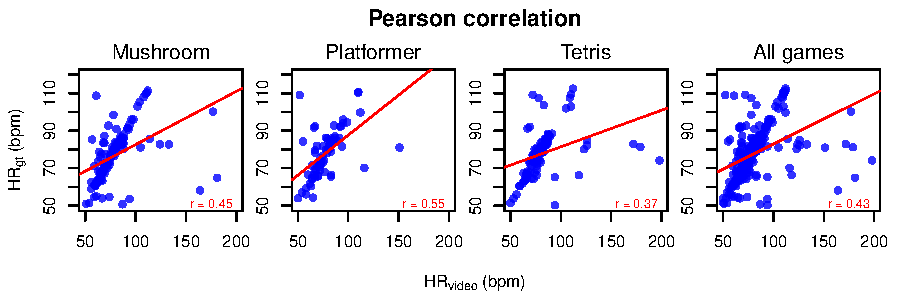
\includegraphics[width=\columnwidth]{Content/figures/correlation-hrgt-hrvideo.pdf}
\caption{Statistical correlation of $HR_{gt}$ and $HR_{video}$ when applied to the video segments of each game, as well as to the video segments of all games.}
\label{fig:chart-r-games}
\end{figure}

To better analyze the variations regarding estimation errors among subjects, figures \ref{fig:chart-hists-me} and \ref{fig:chart-hists} show a distribution of values of $M_e$, RMSE and $M_{eRate}$ for all games combined and individually. The x-axis represents intervals of values of $M_e$, RMSE or $M_{eRate}$ while the y-axis represents the percentage of subjects that presented an estimation error within the interval informed in the x-axis.

Regarding the distribution of values of $M_e$, shown in Figure \ref{fig:chart-hists-me}, overall 66.1\% of the subjects presented estimations with $M_e$ within the interval [-5 bpm, 5 bpm]. For the remaining 33.9\% of the subjects, $M_e$ was spread within the interval [-20 bpm, 35 bpm]. On a game level, $M_e$ was within the interval [-5 bpm, 5 bpm] for 65\%, 68.4\% and 65\% of the subjects of the Mushroom, Platformer and Tetris game, respectively. The values for $M_e$ are more equally distributed for the Platformer game, which explains the lower values of $SD_e$ for that game when compared to the Mushroom and the Tetris game, which present less equally distributed values of $M_e$.

The distribution of values of RMSE, shown in Figure \ref{fig:chart-hists} in the first row, indicate that overall values were lower then 10 bpm for 59.4\% of the subjects, while the remaining of the subjects had RMSE varying from 10 bpm to 50 bpm. On a game level, RMSE was lower than 10 bpm for 50\%, 68.5\% and 60\% of the subjects of the Mushroom, Platformer and Tetris game, respectively.

Regarding $M_{eRate}$, shown in Figure \ref{fig:chart-hists} in the second row, overall 69.5\% of subjects had HR estimations that were up to 10\% different than the expected HR from ground truth. On a game level, in total 73.7\% and 70\% of the estimations performed by the rPPG technique during the Platformer and the Tetris game, respectively, presented $M_{eRate}$ interior or equal to 10\%. Those values are slightly better than the 65\% of the subjects with $M_{eRate}$ up to 10\% in the Mushroom game. Despite the fact that $M_{eRate}$ was similar for both the Platformer and Tetris games, the former presented no subjects whose $M_{eRate}$ was greater than 30\%, while the later presented 10\% of the subjects with $M_{eRate}$ greater than 30\%.

\begin{figure}[!h]
\centering
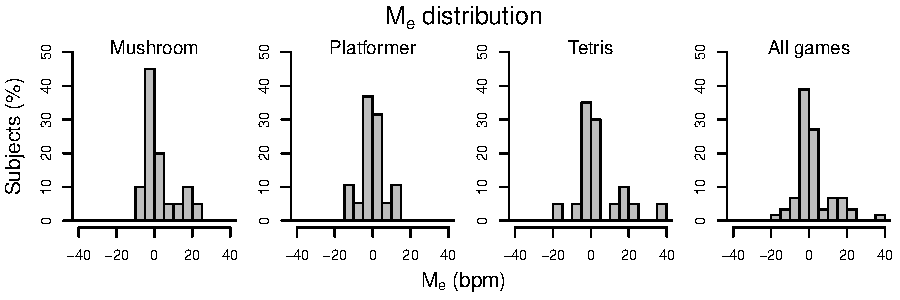
\includegraphics[width=1.0\textwidth]{Content/figures/hist-me.pdf}
\caption{Distribution of values of $M_e$ for all games. The x-axis represents intervals of values of $M_e$ while the y-axis represents the percentage of subjects that presented an estimation error within the interval informed in the x-axis.}
\label{fig:chart-hists-me}
\end{figure}

\begin{figure}[!h]
\centering
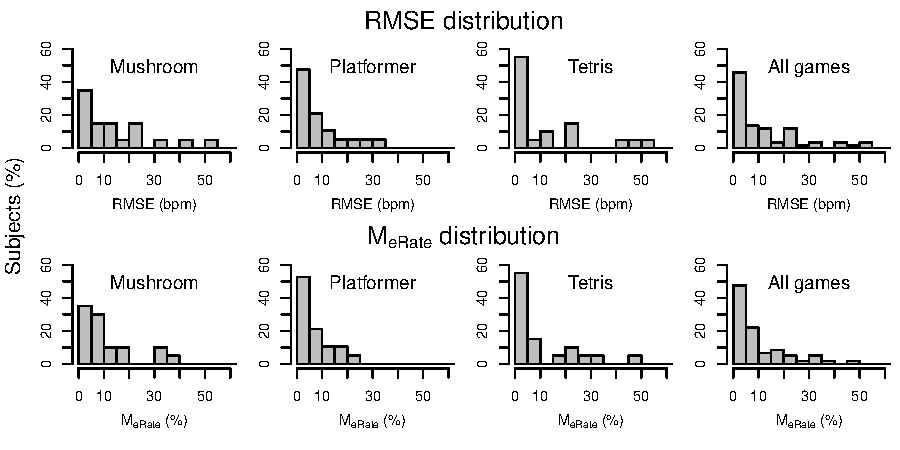
\includegraphics[width=1.0\textwidth]{Content/figures/hist-rmse-mrate.pdf}
\caption{Distribution of values of RMSE and $M_{eRate}$ for all games. The x-axis represents intervals of values of RMSE or $M_{eRate}$ while the y-axis represents the percentage of subjects that presented an estimation error within the interval informed in the x-axis.}
\label{fig:chart-hists}
\end{figure}

\subsection{Discussion}

The results obtained indicate that the use of the selected rPPG technique to estimate HR from videos of gaming sessions is feasible. When the technique was applied to a testing set of 20 manually selected 30 seconds long video segments, whose subject's facial activity and body movement were minimal, the estimations were significantly accurate. As demonstrated by Table \ref{table:rppg-validation}, the mean of error-rate $M_{eRate}$ was 1.52\% and the Pearson's correlation coefficient was $r = 0.99$ for that testing set. Those results were expected since the videos featured an unrealistic condition where subjects remained mostly still with a neutral face.

When the rPPG technique was applied to all gaming sessions, however, body movement and facial activity significantly impacted the estimation performance. It is aligned with previously described works in the literature, which indicate the estimation error increases when subject activities increase \parencite{Wang_2016novel}.

The elevated values for $SD_e$, the standard deviation of $M_e$, suggest significant variations in the estimations among subjects in each video segment. The estimation discrepancies do not seem to be caused by errors equally spread among all gaming sessions, but due to a subset of problematic ones instead. The discrepancies and skewness of the estimations are visible in the scatter plot of the estimated and expected HR values in Figure \ref{fig:chart-r-games}. It shows a cluster of points for each game, however it is surrounded by significantly wrong estimation points. In the Mushroom game, for instance, 5 estimations (bottom right of the chart) were in the interval [120 bpm, 181 bpm] bpm, which is significantly outside the expected ground truth interval of [80 bpm, 110 bpm]. Similar significantly wrong estimations can also be seen in the Platformer and the Tetris game.

The skewed distribution of values of $M_e$, $M_{eRate}$ and RMSE illustrated in figures \ref{fig:chart-hists-me} and \ref{fig:chart-hists} also support that indication. Considering the estimations for all games, in total 69.5\% of them presented $M_{eRate}$ related to an estimation value that was less than 10\% different than the expected HR from ground truth. Additionally 59.4\% of all estimations presented RMSE lower than 10 bpm. That result is slightly worse when compared to similar works that used rPPG techniques and subjects featuring natural movements, whose reported RMSE was between 0.11 and 7.28 bpm.

A direct comparison of the results of this study to the ones of such similar works is unfair however. Despite the fact that the aforementioned works present experiments where subjects are told to behave naturally, their accuracy evaluation is based on artificial human-computer interactions, as previously described in Section \ref{s:experiment1-study3}. The accuracy results of the present study account for body and facial movement caused by games whose focus is entertainment, not artificial interactions. As a consequence, the results are more connected to a scenario involving real and spontaneous reactions to games, showing that the estimations of the rPPG technique are feasible, however skewed by other factors such as natural facial activity and subject movement.

The differences in estimation also seem to be connected to the particularities of each game and subject. Considering the distribution of values of RMSE and $M_{eRate}$, both the Platformer and the Tetris games presented more estimations with lower error than the Mushroom game. The Mushroom game presented 15\% of its estimations with RMSE greater than 30 bpm and $M_{eRate}$ greater than 30\%, which are significantly wrong estimations.

In order to further explore such differences in estimations, the variations of movement and size of the ROI used to track the subject's face along the videos was analyzed. A stable ROI (both in shape and movement) is required for a precise extraction of the plethysmographic signal, so significant variations in the ROI lead to estimation errors. The mean position of the center point of the ROI for each subject in each gaming session was calculated. For each subject in each game session, the Euclidean distance between the center point of the ROI of each frame and the mean center point of the ROI previously calculated (for that subject in that session) was measured.

Similarly the mean length of the ROI diagonal for each subject in each game session was calculated, subtracting it from the length of the ROI diagonal of each frame in that gaming session. Since game sessions differ in time duration, the subject's progress in the game was normalized using the interval [0, 1], where 0 is the start point of the gaming session and 1 its end. Measurements were also subtracted from the sessions mean to facilitate analysis and comparison among different games/subjects.

\begin{figure}[!h]
\centering
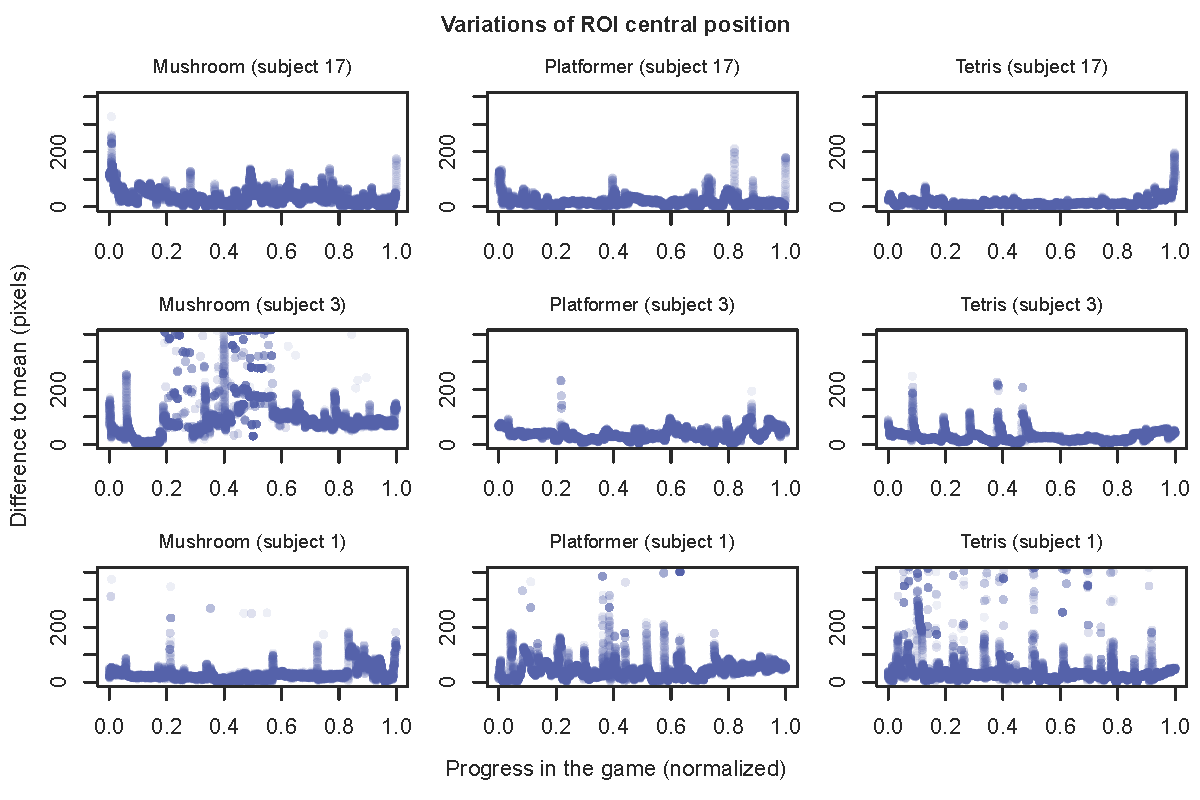
\includegraphics[width=\textwidth]{Content/figures/variation-roi-center.png}
\caption{Variations of distance of the ROI central position for subjects 17 (low estimation errors), 3 (moderate to high estimation errors) and 1 (high estimation errors) during their gaming sessions. Values were subtracted from session mean to facilitate analysis and comparison among different games/subjects.}
\label{fig:chart-roi-anomalies-center}
\end{figure}

Figure \ref{fig:chart-roi-anomalies-center} illustrates some of the patterns observed in the investigation of the distance of the ROI central position. Each row in the figure contains three charts showing the variations of the ROI central position along the gaming sessions of a given subject. The first row contains the investigation of subject 17, who presented, for all his/her gaming sessions combined, -0.33 for $M_e$ ($SD_e$ 1.4) and 1.39 for RMSE (low estimation errors). The second row shows subject 3, who presented 11.47 for $M_e$ ($SD_e$ 16.47) and 19.62 for RMSE (moderate to high estimation errors). Finally the third row shows subject 1, who presented 15.94 for $M_e$ ($SD_e$ 28.5) and 31.96 for RMSE (high estimation errors).

The estimations performed on subject 17 were significantly accurate and the charts regarding the variation of the ROI central position show a stable progression along all gaming sessions. The distance variation (y-axis) remains mostly concentrated within the interval of [0, 100] pixels for all games, which suggest the subject presented few or short movements during gaming sessions. Subject 3 also presented low variation in the Platformer and the Tetris game, however there is a significant variation in the ROI central position in the Mushroom gaming session. The chart indicates significant distance variations of the ROI that are above 200 pixels in a certain period of the game. Finally subject 1 presents high variations in the ROI distance in all gaming sessions, as demonstrated by points above the 200 pixels mark regarding the difference to mean. The Tetris game, in special, present distance variations above 200 pixels during almost the whole session.

\begin{figure}[!h]
\centering
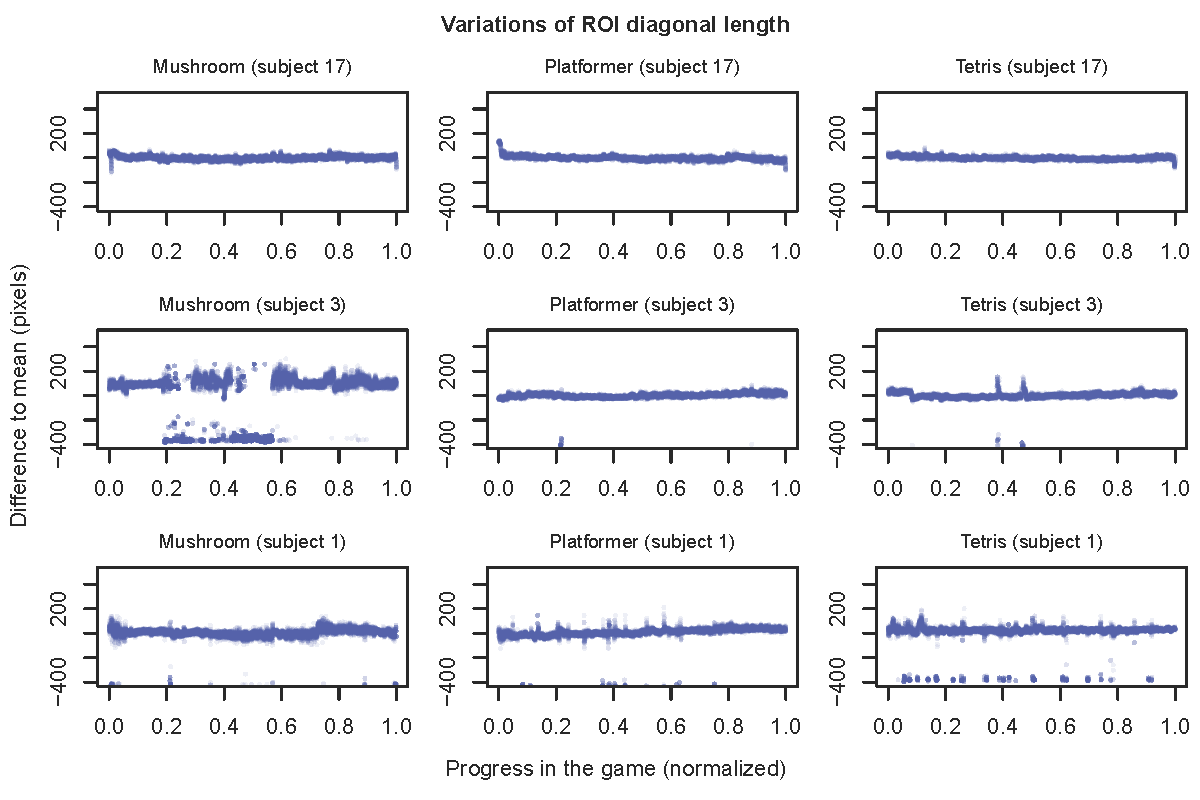
\includegraphics[width=\textwidth]{Content/figures/variation-roi-diagonal.png}
\caption{Variations of ROI diagonal length for subjects 17 (low estimation errors), 3 (moderate to high estimation errors) and 1 (high estimation errors) during their gaming sessions. Values were subtracted from session mean to facilitate analysis and comparison among different games/subjects.}
\label{fig:chart-roi-anomalies-diagonal}
\end{figure}

Figure \ref{fig:chart-roi-anomalies-diagonal} illustrates the same subjects regarding the investigation of the variations of the ROI diagonal length. Similarly to the variations of the ROI central position, the variation of the ROI diagonal length (y-axis) is lower for subject 17 (first row of charts in the figure), since the majority of the values are close to zero. Subject 3 also presents low variations in the ROI diagonal length during the Platformer and the Tetris game, however there are significant changes in the ROI size during a period in the Mushroom game. In such period, the length of the ROI diagonal is negative, i.e. -400 pixels, which indicates the size of the detected ROIs for those frames was smaller than the mean ROI diagonal length. It could be caused by a wrongly detected face (false-negative), for instance. Finally subject 1 presents, to some extent, variations of the ROI diagonal length during the majority of his/her gaming sessions. Those constant variations could be caused by the inability of the face tracking algorithm to stably and continuously detect the subjects face along the frames of the video. The chart shows a distribution of values along the zero mark regarding difference to mean, however they are more spread than those of subject 17, for instance, which indicates higher instability of the ROI size/detection for subject 1. In the Tetris session of subject 1, for instance, there are extreme variation in the ROI diagonal length with values close to -400 pixels, similarly to the ones of subject 3 in the Mushroom game. Such extreme variation could also be explained by a wrongly detected face area during those frames.

An inspection of the videos of subjects with patterns similar to the ones of subjects 3 and 1 revealed sensitive amount of movement and facial activity, including occlusion of the face by the subject's hand, as illustrated by Figure \ref{fig:face-variation}. Any facial occlusion influences the face tracking algorithm used (Viola\&Jones), since it might wrongly detect the face position or do not detect it at all. A flawed face detection step affects the extraction of the plethysmographic signal, because noise is extracted along with the raw signal, making the rPPG technique unable to separate it properly.

Despite the efforts to create games that prevented face occlusion by the subject's hand, such behavior seems to be natural in boring situations. Both Mushroom and Tetris games were more likely to allow players to place a hand in the face to express boredom, since the games could still be played with a single hand when the gameplay speed was not elevated. The Platformer game, on the other hand, is less likely to allow players to use only a single hand to play, which reduced chances of face oclusion inferering with the face tracking algorithm. This could also explain why estimations made during the Platformer game were more accurate than those performed during the other two games. Those extreme cases with facial occlusion are probably affecting the error rates in the analysis, producing less accurate estimations. Such extreme and flawed cases could have removed from the analysis, however the aim is to test how the selected rPPG technique performs in natural gaming situations. A dataset with untreated videos of gaming sessions with natural interactions might produce sub-optimal HR estimations, however it is the understanding that stressing the rPPG technique with less artificial videos provides researchers with insights about possible problems and accuracy limits of such tool.

\begin{figure}
\centering
  \begin{subfigure}[b]{0.5\textwidth}
    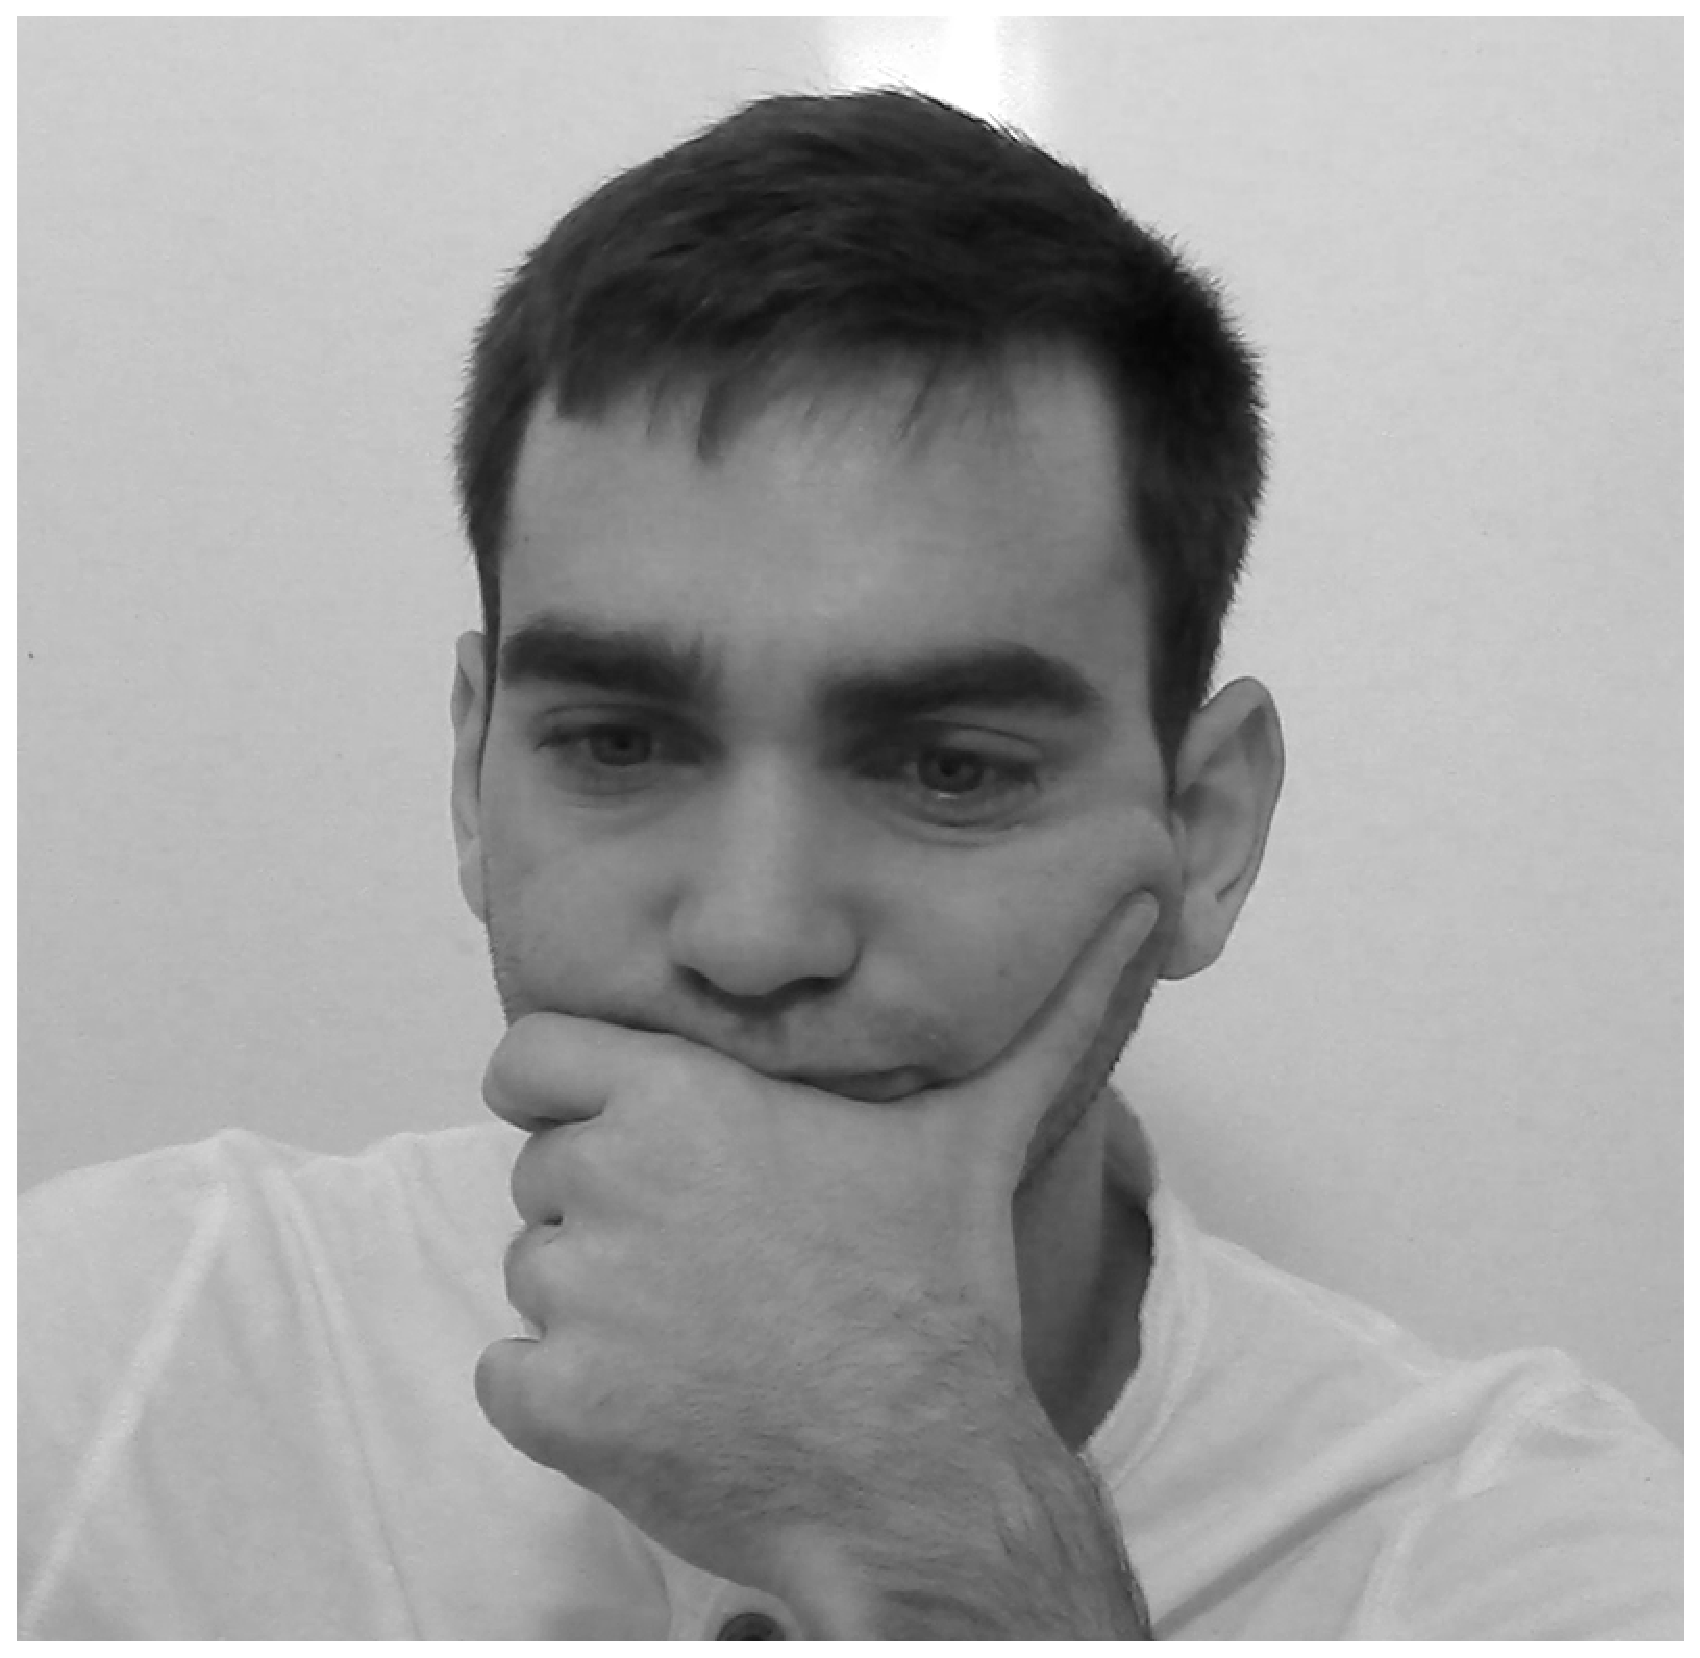
\includegraphics[width=0.95\textwidth]{Content/figures/face-occlusion}
    \caption{}
    \label{fig:face-occlusion}
  \end{subfigure}%
  \begin{subfigure}[b]{0.5\textwidth}
    \centering
    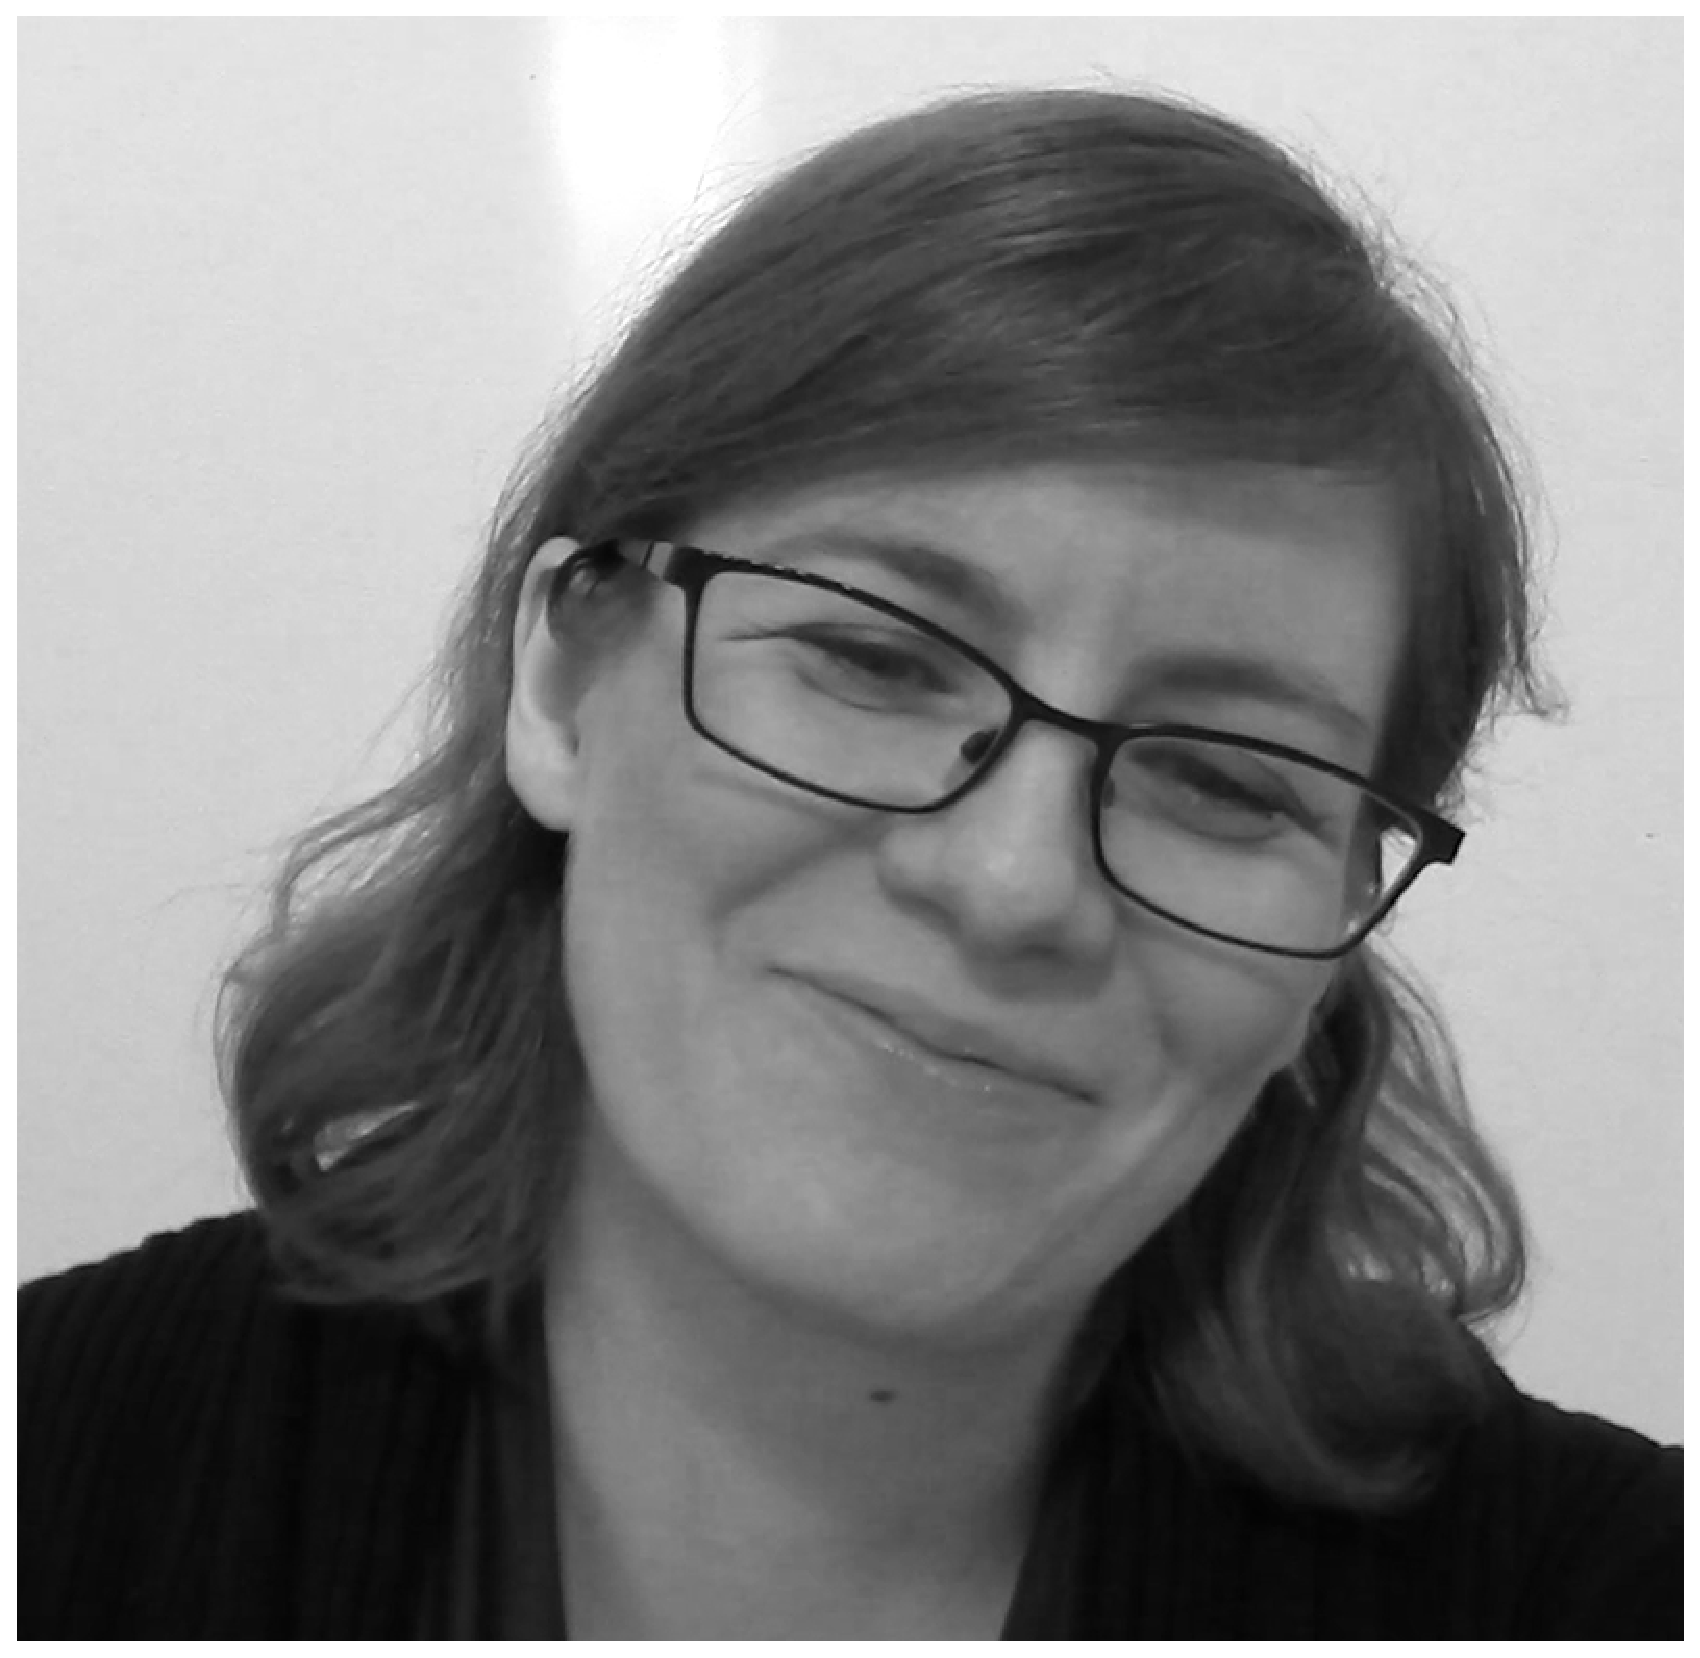
\includegraphics[width=0.95\textwidth]{Content/figures/head-tilt}
    \caption{}
    \label{fig:head-tilt}
  \end{subfigure}
  \caption{Examples of body movement and facial activity during gaming sessions. (a) Partial face occlusion by subject's hand; (b) Head tilt and movement during laugh action.}
  \label{fig:face-variation}
\end{figure}

It is possible to speculate that the variations regarding movement and size of the ROI, which directly influence estimation accuracy of the rPPG technique, seem to be connected to the unique behavior of each user as well. As illustrated by Figures \ref{fig:chart-roi-anomalies-center} and \ref{fig:chart-roi-anomalies-diagonal}, subjects present different movement patterns. Previous analysis of the videos indicates significant differences regarding facial activities among subjects \parencite{bevilacqua2016variations}. It strengthens the idea of a user-tailored model able to deal with such peculiarities, which is more likely to produce better estimations. A method that operates its estimations based on the average user behavior is prone to be significantly affected by specific user behavior outside the expected mean pattern, causing skewed distribution of estimation errors such as the ones presented on Figure \ref{fig:chart-hists} regarding $M_{eRate}$ and RMSE.

%\subsection{Limitations}

%Some limitations of the experimental procedure and analysis should be noted. The 1-minute long duration of each video segment used for the estimation of HR may affect the results. The ideal length of the video segment used for estimation (called window size) is not agreed upon in the literature \parencite{rouast2016remote}. In general, it depends on the characteristics of the rPPG technique being applied as well as the hardware configuration, such as camera framerate \parencite{roald2013estimation}. We selected a 1 min analysis window based on the information of the original work by \textcite{poh2011advancements}. Additionally our experimental procedure consists of games whose difficulty level changes every 1 minute, so that value is aligned with the window size used for HR estimation. As previously described, the statistical nature of ICA, part of the selected rPPG employed in the experiment, demands longer video samples to produce accurate results. The longer the video, however, the higher the chances of subject motion, which increases noise. A trade-off between the duration of the video segments and the estimation accuracy could be better investigated. Our experimental setup used an external light source to minimize noise caused by changes in illumination, which should narrow the estimation error to causes as subject movement and/or facial activity. It is likely, however, that other factors might impact the estimation accuracy, such as facial hair, e.g. beard and hair over the forehead area, use of glasses, and skin color.

\subsection{Conclusions}

Overall the estimation of the rPPG was feasible, showing mean estimation error of 2.99 bpm (SD 18.83 bpm), RMSE of 19.03 bpm and a positive and medium strength Pearson correlation of $r=0.43$, $p < 0.001$. On average, the estimation error of the rPPG technique was up to 10.31\% of the expected value calculated from ground truth. Additionally the exploratory investigation regarding factors that impacted the accuracy of the rPPG technique, such as variations in the region of interest (ROI) used to remotely extract the HR signal, suggest factors connected to the type of the game being played and the unique behavior of each subject influenced the estimations. Among the causes of such influence were identified body movement, e.g. head tilt and rotation, and facial occlusion by subjects hand.

\section{Study 4: automated facial analysis}
\label{sec:experiment1-study4}

This study presents a method for the automated analysis of facial cues from videos, as well as an empirical evaluation of its application as a potential tool for detecting stress and boredom in players. The proposed automated facial analysis is based on the measurement of facial features ($F_1$ to $F_7$) calculated from facial landmarks obtained unobtrusively via computer vision.

%This study introduces a method for automated analysis of facial cues from videos, presenting empirical results of its application as a potential tool for detecting stress and boredom of players in games. The method is based on Euclidean distances between automatically detected facial points, not relying on prior model training to produce results. Additionally the method is able to cope with face analysis under challenging conditions, such as when players behave naturally, e.g. moving and laughing while playing games. The method was applied on the video recordings to contextualize the automated facial analysis in a more game-oriented fashion than previous work.

%%%%%%%%%%%%%%%%%%%%%%%%%%%%%%%%%%%%%%%%%%%%%%%%%%%%%%%%%%%%%%%%%%%%%%%%%%%%%%%%%%%%%
\subsection{Facial features}
\label{sec:experiment1-study4-features-extraction}

The proposed automated facial analysis is based on the measurement of 7 facial features calculated from 68 detected facial landmarks. Table \ref{table:features} presents the facial features, which are illustrated in Figure \ref{fig:faces}(b). The facial features are mainly based on the Euclidean distances between landmarks, similar to some works previously mentioned. However, the approach does not rely on pre-defined expressions, i.e. the 6 universal facial expressions, training of a model, or the use of the MPEG-4 standard, which specifies representations for 3D facial animations, not emotional interactions in games. Additionally the method does not use an arbitrarily selected frame, e.g. the 100\textsuperscript{th} frame \parencite{giannakakis2017stress}, as a reference for calculations, since features are derived from each frame (or a small set of past frames). The features are obtained unobtrusively via computer vision analysis that focuses on detecting activity of facial muscles reported by previous work involving EMG and emotion detection in games.
%We believe our approach is more user-tailored, convenient and better suited for contexts involving games.

The process of extracting the facial features has two main steps: face detection and feature calculation. In the first step, computer vision techniques are applied to a frame of the video and facial landmarks are detected. In the second step, the detected landmarks are used to calculate several facial features related to eyes, mouth, and head movement. The following sections present a detailed description of how each step is performed, including the calculation of features.

% zygomatic -> smiling
% orbicularis oculi -> eyelid control
% corrugator -> frowning

\begin{landscape}
\begin{table*}
    \centering
    \caption{Information regarding calculated facial features}
    \label{table:features}
    \begin{tabular}[l]{@{}lcp{11cm}}
        \toprule%
            \textbf{Name} & \textbf{Notation} & \textbf{Description} \\
        \midrule%
            Mouth outer & $F_1$ & Sum of the Euclidean distance between the mouth contour landmarks and the anchor landmarks. It monitors the zygomatic muscle.  \\
            Mouth corner & $F_2$ & Sum of the Euclidean distance between the mouth corner landmarks and the anchor landmarks. It monitors the zygomatic muscle. \\
            Eye area & $F_3$ & Area of the regions bounded by the closed curves formed by the landmarks in the contour of the eyes. It monitors the orbicularis oculi muscle. \\
            Eyebrow activity & $F_4$ & Sum of the Euclidean distance between eyebrow landmarks and the anchor landmarks. It monitors the corrugator muscle.  \\
            Face area & $F_5$ & Area of the region bounded by the closed polygon formed by the most external detected landmarks.  \\
            Face motion & $F_6$ & Average value of the Euclidean norm of a set of landmarks in the last $N$ frames. It describes the total distance the head has moved in any direction in a short period of time.  \\
            Facial COM & $F_7$ & Average value of all detected landmarks. It describes the overall movement of all facial landmarks.  \\
        \bottomrule%
    \end{tabular}
\end{table*}
\end{landscape}

%%%%%%%%%%%%%%%%%%%%%%%%%%%%%%%%%%%%%%%%%%%%%%%%%%%%%%%%%%%%%%%%
\subsubsection{Face detection}

The face detection procedure is performed for every frame of the input video. Initially the face is detected using a Constrained Local Neural Field (CLNF) model \parencite{baltrusaitis2013constrained,baltruvsaitis2016openface}. CLNF uses a local neural field patch expert that learns the nonlinearities and spatial relationships between pixel values and the probability of landmark alignment. The technique also uses a non-uniform regularized landmark Mean Shift fitting technique that takes into consideration patch reliabilities. It improves the detection process under challenging conditions, e.g. extreme face pose or occlusion, which is likely to happen in game sessions (see Section \ref{sec:experiment1-study1}). The application of the CLNF model to a given video frame produces a vector $L$ of 68 facial landmarks:

\[
L = [p_0, p_1, p_2, \dots, p_{67}]^T
\]

where $p_i$ is a detected facial landmark that represents a 2D coordinate $(x_i, y_i)$ in the frame. Facial landmarks are related to different facial regions, such as eyebrows, eyes and lips. Figure \ref{fig:faces}(a) illustrates the landmarks of $L$ in a given frame.

\begin{figure}
\centering
  \begin{subfigure}[b]{0.5\textwidth}
    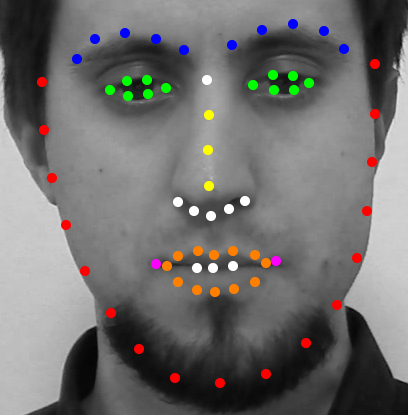
\includegraphics[width=0.95\textwidth]{Content/figures/facial-landmarks-detail.png}
    \caption{}
    \label{fig:facial-landmarks}
  \end{subfigure}%
  \begin{subfigure}[b]{0.5\textwidth}
    \centering
    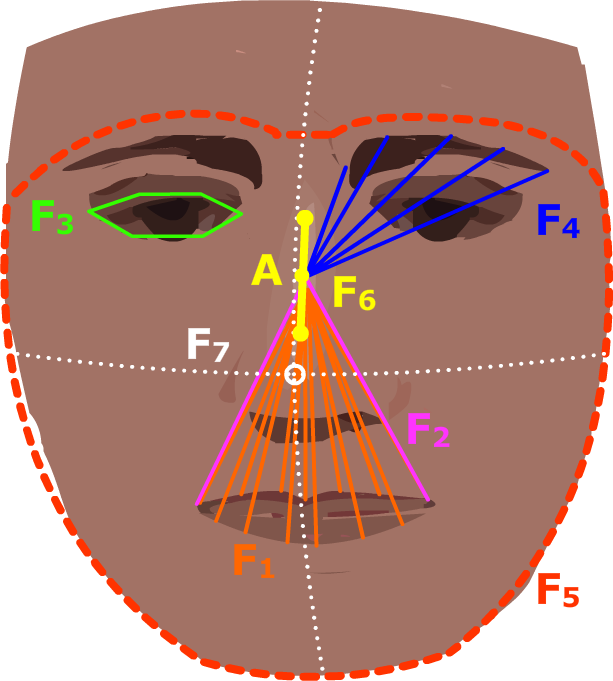
\includegraphics[width=0.95\textwidth]{Content/figures/facial-features.png}
    \caption{}
    \label{fig:facial-features}
  \end{subfigure}
  \caption{Facial landmarks and features. (a) Highlight of 68 detected facial landmarks. (b) Visual representation of the facial features.}
  \label{fig:faces}
\end{figure}


%%%%%%%%%%%%%%%%%%%%%%%%%%%%%%%%%%%%%%%%%%%%%%%%%%%%%%%%%%%%%%%%
\subsubsection{Anchor landmarks}

The calculation of the proposed facial features involves the Euclidean distance among facial landmarks. Subsequently, the Euclidean distance between two landmarks $a_1 = (x_1, y_1)$ and $a_2 = (x_2, y_2)$ is given as:

\[
d(a_1,a_2) = \sqrt{(x_2 - x_1)^2 + (y_2 - y_1)^2}
\]

Landmarks in the nose area are more likely to be stable, presenting fewer position variations in consecutive frames \parencite{giannakakis2017stress}. Consequently, they are good reference points for use in the calculation of the Euclidean distance among landmarks. In order to provide stable reference points for the calculation of our facial features, three highly stable landmarks located in the nose line were selected, denoted as the anchor vector $A = [p_{28}, p_{29}, p_{30}]^T$. The landmarks of the anchor vector $A$ are highlighted in yellow in Figure \ref{fig:faces}(a).

%%%%%%%%%%%%%%%%%%%%%%%%%%%%%%%%%%%%%%%%%%%%%%%%%%%%%%%%%%%%%%%%
\subsubsection{Feature normalization}

The subjects moved towards and away from the camera during the gaming sessions. This movement affects the Euclidean distance between landmarks, as it tends to increase when the subject is closer to the camera, for instance. Additionally, the subjects have unique facial shapes and characteristics, which also affect the calculation and comparison of the facial features between subjects. To mitigate that problem, a normalization coefficient $K$ was calculated as the Euclidean distance between the upper and lower-most anchor landmarks in $A$. In other words, $K$ represents the size of a subject's nose line. Since all features are divided by $K$, their final value is expressed as normalized pixels (relative to $K$) rather than pixels \textit{per se}.

%%%%%%%%%%%%%%%%%%%%%%%%%%%%%%%%%%%%%%%%%%%%%%%%%%%%%%%%%%%%%%%%
\subsubsection{Mouth related features}

Mouth related features aim to detect activity in the zygomatic muscles, illustrated in Figure \ref{fig:face-muscles} (c and d, page \pageref{fig:face-muscles}), which are related to changes in the mouth, such as lips activity (stretch, suck, press, parted, tongue touching, bite) and movement (including talking). Two facial features related to the mouth area were calculated: mouth outer and mouth corner.

\paragraph{Mouth outer ($F_1$):} given vector $M = [p_{48}, p_{49}, \dots, p_{60}]^T$ containing the landmarks in the outer part of the mouth (highlighted in orange in Figure \ref{fig:faces}(a)). The mouth outer feature is calculated as the sum of the Euclidean distance among the landmarks in $M$ and the anchor landmarks in $A$:

\[
F_1 = \frac{1}{K} \sum_{i=1}^{12} \sum_{j=1}^{3} d(A_j, M_i)
\]

where $A_j$ and $M_i$ are the $j$-th and $i$-th element of $A$ and $M$, respectively.

\paragraph{Mouth corner ($F_2$):} given vector $C = [p_{48}, p_{54}]^T$, containing the two landmarks representing the mouth corners (highlighted in pink in Figure \ref{fig:faces}(a)). The mouth corner feature is the sum of the Euclidean distance among the landmarks in $C$ and $A$:

\[
F_2 = \frac{1}{K} \sum_{i=1}^{2} \sum_{j=1}^{3} d(A_j, C_i)
\]

where $A_j$ and $C_i$ are the $j$-th and $i$-th element of $A$ and $C$, respectively.

%%%%%%%%%%%%%%%%%%%%%%%%%%%%%%%%%%%%%%%%%%%%%%%%%%%%%%%%%%%%%%%%
\subsubsection{Eye related features}

Eye related features aim to detect activity related to the orbicularis oculi and the corrugator muscles, illustrated in Figure \ref{fig:face-muscles}(b) and Figure \ref{fig:face-muscles}(a) respectively, which comprehend changes in the eyes region, including eye and eyebrow activity. Two facial features related to the eyes were calculated: eye area and eyebrow activity.

\paragraph{Eye area ($F_3$):} given vector $Y_l = [p_{36}, p_{37}, \dots, p_{41}]^T$ containing the landmarks describing the left eye, highlighted in green in Figure \ref{fig:faces}(a), and vector $Y_r = [p_{42}, p_{43}, \dots, p_{47}]^T$ containing the landmarks describing the right eye, highlighted in green in Figure \ref{fig:faces}(a). The eye area feature is the area of the regions bounded by the closed curves formed by the landmarks in $Y_l$ and $Y_r$, divided by $K$. The area of the curves is calculated using OpenCV's \texttt{contourArea()} function, which uses Green's theorem \parencite{stewart2011calculus}.

\paragraph{Eyebrow activity ($F_4$):} calculated as the sum of the Euclidean distances among the eyebrow landmarks and the anchor landmarks in $A$. Given the vector $W_l = [p_{17}, p_{18}, \dots, p_{21}]^T$ containing the landmarks describing the left eyebrow, highlighted in blue in Figure \ref{fig:faces}(a), and the set $W_r = [p_{22}, p_{23}, \dots, p_{26}]^T$ containing the landmarks describing the right eyebrow, highlighted in blue in Figure \ref{fig:faces}(a). The eyebrow activity feature is calculated as:

\[
F_4 = \frac{1}{K} \sum_{i=1}^{5} \sum_{j=1}^{3} \Big[ d(A_j, W_{l,i}) + d(A_j, W_{r,i}) \Big]
\]

where $A_j$, $W_{l,i}$ and $W_{r,i}$ are the $j$-th, $i$-th and $i$-th element of $A$, $W_l$ and $W_r$, respectively.

%%%%%%%%%%%%%%%%%%%%%%%%%%%%%%%%%%%%%%%%%%%%%%%%%%%%%%%%%%%%%%%%
\subsubsection{Head related features}

Head related features aim to detect body movements, in particular, variations of head pose and amount of motion the head/face performs over time. Three features related to the head were calculated: face area, face motion and facial center of mass (COM).

\paragraph{Face area ($F_5$):} during the interaction with a game, subjects tend to move towards (or away from) the screen, which causes the facial area in the video recordings to increase or decrease. Given vector $F = [p_{0}, p_{1}, \dots, p_{16}]^T$ containing the landmarks describing the contour of the face, highlighted in red in Figure \ref{fig:faces}(a). The face area feature is the area of the region bounded by the closed curves formed by the landmarks in $F \cup W_r \cup W_l$, divided by $K$. Similar to the eye area, the area under the curves is calculated using OpenCV's \texttt{contourArea()} function.

\paragraph{Face motion ($F_6$):} accounts for the total distance the head has moved in any direction in a short period of time. For each frame of the video, the currently detected anchor vector $A$ is saved, which produces vector $D = [A_1, A_2, \dots, A_n]^T$, where $A_i$ is the vector $A$ detected in the $i$-th frame of the video and $n$ is the number of frames in the video. Subsequently the face motion feature is calculated as:

\[
F_6 = \frac{1}{K} \sum_{j=1}^{3} \sum_{t=1}^{Z - 1} || D(f - t, j) - D(f - Z, j) ||
\]

where $Z$ is the number of frames to include in the motion analysis, $D(i,j)$ is the $j$-th element of $A_i \in D$, $f$ is the number of the current frame, and $||.||$ is the Euclidean norm. In the analysis presented here, a value of $Z=50$ (50 frames, equivalent to 1 second) was used.

\paragraph{Facial COM ($F_7$):} describes the overall movement of all facial landmarks. A single 2D point, calculated as the average of all landmarks in $L$, is used to monitor the movement. The COM feature is calculated as:

\[
F_7 = \frac{1}{K} \frac{1}{N} \sum_{i=1}^{N} || p_i ||
\]

where $N$ is the total number of detected landmarks (elements in $L$) and $||.||$ is the Euclidean norm.

%%%%%%%%%%%%%%%%%%%%%%%%%%%%%%%%%%%%%%%%%%%%%%%%%%%%%%%%%%%%%%%%
\subsection{Analysis and methods}
\label{sec:experiment1-study4-feature-analysis}

%%%%%%%%%%%%%%%%%%%%%%%%%%%%%%%%%%%%%%%%%%%%%%%%%%%%%%%%%%%%%%%%
\subsubsection{Data pre-processing}

The pre-processing of video recordings involved the extraction of parts containing the interaction with the games and the discarding of noisy frames. Firstly, the periods showing subjects playing each available game were extracted from the video recordings. This resulted in three videos per subject, denoted as $V_{s,i}$ where $s$ is the $s$-th subject and $i \in \{1, 2, 3\}$ represents the game.

\begin{figure}
\centering
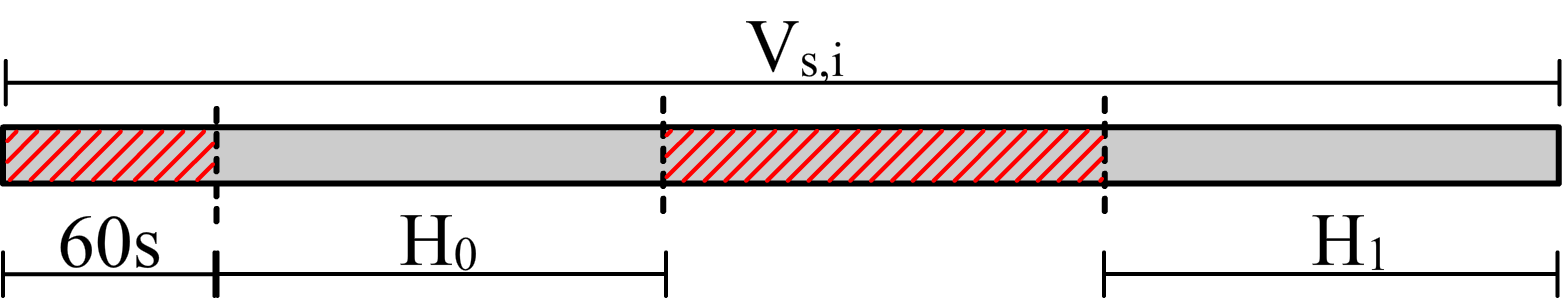
\includegraphics[width=0.7\textwidth]{Content/figures/pre-processing}
\caption{Extraction of video segments $H_0$ and $H_1$ containing boring and stressful game interactions, respectively. Initial $D$ seconds of any video $V_{s,i}$ are ignored and the remaining is divided into three pieces, from which the first and the last ones are selected. Stripes highlight discarded video segments.}
\label{fig:preprocessing}
\end{figure}

As previously mentioned, the games used as emotional elicitation material in the experiment induced variations of physiological signals in the subjects, who perceived the games boring at the beginning and stressful at the end. Since the aim of the present study was to test the potential of facial features to differentiate emotional states of boredom and stress, two video segments were extracted from each video $V_{s,i}$, named $H_0$ and $H_1$, whose subject's emotional state was assumed to be known and related to boredom and stress. In order to achieve that, the following extraction procedure was performed, illustrated in Figure \ref{fig:preprocessing}. Firstly a duration of $D$ seconds of any given video $V_{s,i}$ was ignored. For this pre-processing, $D=60$ was used. The remainder of the video was then divided into three segments, from which the first and the last were selected as $H_0$ and $H_1$, respectively.

The reason $D=60$ seconds was discarded from all the video's segments is because the initial minute might not be ideal for a fair analysis. During the first minute of gameplay, subjects are less likely to be in their usual neutral emotional state. They are more likely to be stimulated by the excitement of the initial contact with a game soon to be played, which interferes with any feelings of boredom. Additionally, subjects need basic experimentation with a game to learn how to play it and assess whether it is boring or not. This claim is supported by the empirical analysis of the first minute of the video recordings, which show repeated head and eye movements to and from the keyboard/display. Consequently, the second minute and onward in the videos is more likely to portray facial activity related to emotional reactions to the game than facial activity connected to gameplay learning. Regarding the division of the remaining part of the video into three segments, from which two were selected as $H_0$ and $H_1$, it followed the reasoning that the emotional state of the subjects was unknown in the middle part of $V_{s,i}$. Based on the self-reported emotional states, subjects reported the beginning part of the games as boring and the final part as stressful. Additionally, there are significant differences in the HR mean between the second and the last minute of gameplay in the games \parencite{bevilacqua2018changes}. As a consequence, it is assumed that the video segments $H_0$ and $H_1$ accurately portray the interaction of the subjects during boring and stressful periods of the games, respectively.

The pre-processing of the recordings resulted in 6 video segments per subjects: 3 segments $H_0$ (one per game) and 3 segments $H_1$ (one per game). A given game $i$ contains $N=20$ pairs of $H_0$ and $H_1$ video segments (20 segments $H_0$, one per subject, and 20 segments $H_1$, one per subject). With regard to all the subjects and games, there are $N=60$ pairs of $H_0$ and $H_1$ video segments (3 games $\times$ 20 subjects, resulting in 60 segments $H_0$ and 60 segments $H_1$). Subject 9 had problems playing the Platformer game, consequently, segments $H_0$ and $H_1$ from subject 9 in the Platformer game were discarded. Therefore, the Platformer game contains $N=19$ pairs of $H_0$ and $H_1$ video segments; regarding all the games and subjects, there are $N=59$ pairs of $H_0$ and $H_1$ video segments.

%%%%%%%%%%%%%%%%%%%%%%%%%%%%%%%%%%%%%%%%%%%%%%%%%%%%%%%%%%%%%%%%
\subsubsection{Feature analysis}

The previously mentioned features can be calculated for each frame of any given video, however facial cues might be better contextualized if analyzed in multiple frames. For that reason, the facial analysis was applied to all the frames of all the video segments $H_0$ and $H_1$. The mean value of each facial feature in each video segment was then calculated. As a result, any facial feature $F_i$ has $N=59$ pairs of mean values (59 from $H_0$ and 59 from $H_1$). Henceforth, the set of mean values in $H_0$ or $H_1$ of a given feature $F_i$ will be referred to simply as feature value in $H_0$ or $H_1$, respectively.
%Each mean value was calculated from all frames of a video segment ($H_0$ or $H_1$) of a subject in a particular game.

Based on a previous manual analysis of facial actions of the video recordings \parencite{bevilacqua2016variations} and findings of related work, the values of facial features during boring periods of the games are expected to be different than those during stressful periods. Since the subjects perceived the games as boring at the beginning and stressful at the end, it is assumed that values in $H_0$ and $H_1$, for all features, are likely to correlate with an emotional state of boredom and stress, respectively. Therefore, the overarching hypothesis is stated as follows: the mean value of features in $H_0$ is different than the mean value in $H_1$, for all the subjects and games. More specifically, the overarching hypothesis can be described as 7 sub-hypotheses, denoted $u_i$, where $i \in \{1, 2, ..., 7\}$. Hypothesis $u_i$ states that the true difference in means between the value of a given feature $F_i$ in $H_0$ and $H_1$, for all the subjects, is greater than zero. The dependent variable of $u_i$ is $F_i$ and the null hypothesis is that the true difference in means between $H_0$ and $H_1$ for feature $F_i$, for all the subjects and games, is equal to zero.

Hypothesis $u_i$ was tested by performing a paired two-tail t-test on the values $H_0$ and $H_1$ of feature $F_i$. In total, 7 tests were performed: $u_1$ (mouth outer), $u_2$ (mouth corner), $u_3$ (eye area), $u_4$ (eyebrow activity), $u_5$ (face area), $u_6$ (face motion), and $u_7$ (facial COM).

%%%%%%%%%%%%%%%%%%%%%%%%%%%%%%%%%%%%%%%%%%%%%%%%%%%%%%%%%%%%%%%%%%%%%%%%%%%%%%%%%%%%%
\subsection{Results}
%%%%%%%%%%%%%%%%%%%%%%%%%%%%%%%%%%%%%%%%%%%%%%%%%%%%%%%%%%%%%%%%%%%%%%%%%%%%%%%%%%%%%

Table \ref{table:changes} presents the mean of differences of all the features between periods $H_0$ and $H_1$, calculated for all the subjects in all the games, according to the description in Section \ref{sec:experiment1-study4-features-extraction}, and analyzed according to the procedures described in Section \ref{sec:experiment1-study4-feature-analysis}. The mean of differences of all the features shows a decrease from $H_0$ to $H_1$. Comparing the mean difference of a feature to its mean value in $H_0$, the decrease from $H_0$ to $H_1$ was 10.7\% for mouth outer ($F_1$), 11.8\% for mouth corner ($F_2$), 10.4\% for eye area ($F_3$), 8.1\% for eyebrow activity ($F_4$), 9.4\% for face area ($F_5$), 8.2\% for face motion ($F_6$), and 11\% for facial COM ($F_7$). Changes related to $F_6$ and $F_7$ were not statistically significant. All the remaining features presented statistically significant changes from $H_0$ to $H_1$. The greatest decrease with statistical significance was associated with mouth corner, followed by mouth outer, eye area, face area, and eyebrow activity. These numbers support the experimental expectations that values for facial features are different when a comparison is made between two distinct parts of the games, i.e. boring and stressful ones.

\begin{table}
    \caption{Mean of differences ($\pm$SD) of features between periods $H_0$ and $H_1$ ($N=59$). Units expressed in normalized pixels.}
    \label{table:changes}
    \centering
    \begin{threeparttable}
        \begin{tabular}{lc}
            \toprule%
                \textbf{Feature (notation)} &  \\
            \midrule%
                Mouth outer ($F_1$)      & -20.59 $\pm$ 57.36\textsuperscript{**} \\
                Mouth corner ($F_2$)     & -3.90 $\pm$ 10.16\textsuperscript{**} \\
                Eye area ($F_3$)         & -0.019 $\pm$ 0.064\textsuperscript{*} \\
                Eyebrow activity ($F_4$) & -15.59 $\pm$ 49.71\textsuperscript{*} \\
                Face area ($F_5$)        & -2.60 $\pm$ 7.90\textsuperscript{*} \\
                Face motion ($F_6$)      & -44.97 $\pm$ 326.74 \\
                Facial COM ($F_7$)       & -0.029 $\pm$ 0.113 \\
            \bottomrule%
        \end{tabular}
        \begin{tablenotes}
          \small
          \item[*]{$p < 0.05$}
          \item[**]{$p < 0.01$}
        \end{tablenotes}
    \end{threeparttable}
\end{table}

The two facial features related to mouth, i.e. mouth corner and mouth outer, presented a combined average decrease of 11.24\% from $H_0$ to $H_1$. The change was the most significant compared to all other features. The mean of differences of $F_1$ and $F_2$ between periods $H_0$ and $H_1$ was $T(59) = -20.59$ (SD 57.36, $p < 0.01$) and $T(59) = -3.9$ (SD 10.16, $p < 0.01$), respectively. Both features had a statistically significant change from $H_0$ to $H_1$, which supports the claim that they are different in those periods. Additionally, both features presented SD as considerably greater than the mean, which indicates that the differences of such features for each subject between periods $H_0$ and $H_1$ are likely to be spread out rather than clustered around the mean value.
Features related to eyes, i.e. eye area and eyebrow activity, presented a combined average decrease of 9.28\% from $H_0$ to $H_1$. The mean of differences of $F_3$ and $F_4$ between periods $H_0$ and $H_1$ was $T(59) = -0.019$ (SD 0.064, $p < 0.05$) and $T(59) = -15.59$ (SD 49.71, $p < 0.05)$, respectively. Similar to mouth-related features, eye-related features had a statistically significant change from $H_0$ to $H_1$, indicating that they are different in those periods. Following the same pattern of change for $F_1$ and $F_2$, both features $F_3$ and $F_4$ also presented a SD considerably greater than the mean, also suggesting that the differences of such features for each subject between periods $H_0$ and $H_1$ are likely to be spread out rather than clustered around the mean value.

Finally, features related to the whole face, i.e. face area, face motion, and facial COM, presented a combined average decrease of 9.52\% from $H_0$ to $H_1$. The mean of differences of $F_5$, $F_6$ and $F_7$ were $T(59) = -2.60$ (SD 7.90, $p < 0.05$), $T(59) = -44.97$ (SD 326.74, $p = 0.29$), and $T(59) = -0.029$ (SD 0.113, $p = 0.052$), respectively. Face area was the only feature in this category to present a change that was statistically significant between periods $H_0$ and $H_1$, supporting the idea that $F_5$ is different in those periods. In constrast, $F_6$ and $F_7$ lack statistically significant differences between periods $H_0$ and $H_1$. Similar to facial features related to mouth and eyes, features $F_5$, $F_6$ and $F_7$ presented considerably greater SD than the mean, also suggesting that the differences of such features between periods $H_0$ and $H_1$ are likely to be spread out rather than clustered around the mean value.

%%%%%%%%%%%%%%%%%%%%%%%%%%%%%%%%%%%%%%%%%%%%%%%%%%%%%%%%%%%%%%%%%%%%%%%%%%%%%%%%%%%%%
\subsection{Discussion}
%%%%%%%%%%%%%%%%%%%%%%%%%%%%%%%%%%%%%%%%%%%%%%%%%%%%%%%%%%%%%%%%%%%%%%%%%%%%%%%%%%%%%

The overarching hypothesis states that the mean value of features in $H_0$ is different than the mean value in $H_1$. Furthermore, the overarching hypothesis is composed of 7 sub-hypotheses. i.e. $u_i$, one for each feature $F_i$, where $u_i$ states that the true difference in means between the value of a given feature $F_i$ in $H_0$ and $H_1$, is greater than zero. The majority of the calculated facial features, i.e. mouth outer ($F_1$), mouth corner ($F_2$), eye area ($F_3$), eyebrow activity ($F_4$), and face area ($F_5$), presented statistically significant differences in their mean values when a comparison is made between two distinct parts of the games, i.e. $H_0$ and $H_1$. As previously mentioned, the subjects perceived the first part of the games, i.e. $H_0$, as boring and the second part, i.e. $H_1$, as stressful. The results support the claim of sub-hypotheses $u_1$ to $u_5$, which indicate that facial features $F_1$ to $F_5$ can be differentiated between periods $H_0$ and $H_1$ and can consequentially have the potential to unobtrusively differentiate the emotional states of boredom and stress of players in gaming sessions. The results refute sub-hypotheses $u_6$ and $u_7$, since features $F_6$ and $F_7$ lack statistically significant differences between periods $H_0$ and $H_1$.

Mouth related facial features, i.e. mouth outer ($F_1$) and mouth corner ($F_2$), presented statistically significant differences between boring and stressful parts of the games. Both features are calculated on the basis of the distance between mouth and nose related facial landmarks, which presented a decrease in stressful parts of the games. This decrease could be attributed to landmarks in the upper and lower lips being closer to each other, which could be associated with lips pressing, lips sucking or talking, for instance. Particular to the mouth corner feature, a decrease in distance is the result of the two mouth corners being placed closer to the nose area, which could be associated with smiles or mouth deformation, e.g. mouth corner pull to left/right. Consequentially, a decrease in the mean value of both features suggests greater mouth activity that involves the proximity of mouth landmarks to the nose area in stressful parts of the games compared to boring parts. Such results are aligned with previous studies that show lip pull corner as a frequent facial behavior during gaming sessions \parencite{kaiser1994multi} and talking as an emotional indicator \parencite{blom2014towards}. Additionally, stating that mouth related features were constructed after the zygomatic muscle activity, the results are connected with previous studies that show increased activity of the zygomatic muscle is related to self-reported emotions \parencite{tijs2008dynamic} and their connection to changes in a game \parencite{ravaja20051}.

Eye related features, i.e. eye area ($F_3$) and eyebrow activity ($F_4$), also presented statistically significant differences between boring and stressful parts of the games. They presented a decrease in the mean value from $H_0$ to $H_1$, which points to landmarks detected in the eyes contour becoming closer to each other in $H_1$. This suggests that more pixels in the eyes area were detected during $H_0$ (boring part) than $H_1$ (stressful part). Such numbers might indicate less blinking activity or more wide-open eyes during boring parts of the games. Additionally, they could indicate more blinking and eye tightening activity (possibly related to frowning) during stressful parts. Both indications are aligned with previous findings, which show increased blinking activity (calculated from eye area) in stressful situations \parencite{giannakakis2017stress}. Regarding the eyebrow feature, its calculation is based on the distance between facial landmarks in the eyebrow lines and the nose. A decrease in value indicates a smaller distance between eyebrows and nose, which could be explained by frowning, suggesting that the subjects presented more frowning action during stressful moments of the game. The mean value of eyebrow activity during $H_0$ is greater than during $H_1$, which indicates that the distance between eyebrows and nose was greater during boring parts of the games compared to stressful parts. It could also be the result of more eyebrow risings, e.g. facial expressions of surprise, in boring periods compared to stressful periods. Eye related features were constructed to monitor the activity of the orbicularis oculi and the corrugator supercilii muscles. The results are related to previous work that reports game events affecting the activity of the orbicularis oculi \parencite{ravaja20051} and the corrugator \parencite{hazlett2006measuring} muscles.

Finally, features related to the whole face, i.e. face area ($F_5$), face motion ($F_6$) and facial COM ($F_7$), are partially conclusive. These features are affected by body motion, e.g. head movement and corporal posture, therefore, a decrease in value might indicate less corporal activity during $H_1$ compared to $H_0$. Face area was the only feature in this category to present a change that was statistically significant. The value of the face area feature is directly connected to the subjects' movement towards and away from the camera. A decrease in face area from $H_0$ to $H_1$ suggests that the subjects were closer to the computer screen more often during boring parts of the games than during stressful parts. The facial COM feature also presented a decrease from $H_0$ to $H_1$. This feature is connected to vertical and horizontal movements, performed by the subject's face, that are anchored to a fixed reference point and less influenced by head rotations. Despite presenting a change that is not statistically significant ($p = 0.519$), the decrease of facial COM might be an indication that the subjects were motionless more during stressful periods than during boring periods. The face motion feature also presented a decrease from $H_0$ to $H_1$ that is not statistically significant ($p = 0.294$). This feature accounts for the amount of movement a subject's face performs in a period of 50 frames (dynamic reference point), which is directly affected by vertical, horizontal and rotational movements of the head. A decrease could be associated with moving/rotating the head less often during the analyzed 50 frames periods in $H_1$ than in $H_0$. However, the lack of statistical significance suggests the change is not related to a subject's emotional state, but other factors, such as the inherent behavior associated with game mechanics, i.e. head movement caused by the observation of cards in the Mushroom game. The results lack the statistical significance to replicate the findings of previous work, which relate head movements to changes in games, i.e. failure \parencite{shaker2011game} and frustration \parencite{blom2014towards}, or to stressful situations \parencite{giannakakis2017stress}.

\begin{table}
    \caption{Percentage of change of features from period $H_0$ to $H_1$ in the Mushroom game ($N=20$).}
    \label{table:mushroom}
    \centering
    \begin{threeparttable}
        \begin{tabular}{lccc}
            \toprule%
                \textbf{Feature (notation)} & \textbf{Mean} & \textbf{Min.} & \textbf{Max.} \\
            \midrule%
                Mouth outer ($F_1$)      & -12.9 & -69.1  &  22.1  \\
                Mouth corner ($F_2$)     & -15.0 & -71.6  &  15.5  \\
                Eye area ($F_3$)         & -8.9  & -76.9  &  8.2   \\
                Eyebrow activity ($F_4$) & -8.0  & -72.3  &  9.6   \\
                Face area ($F_5$)        & -11.3 & -74.5  &  18.2  \\
                Face motion ($F_6$)      & 47.2  & -61.3  &  253.8 \\
                Facial COM ($F_7$)       & -12.9 & -81.0  &  9.8   \\
            \bottomrule%
        \end{tabular}
        \begin{tablenotes}
          \small
          \item[]{}
        \end{tablenotes}
    \end{threeparttable}
\end{table}

It could be argued that the characteristics of each game mechanic influence the mean change of features between the two periods. Such argument is particularly true for features that are calculated on the basis of the  subject's body movement, i.e. face area, face motion and facial COM. In that case, subjects could move the face as a result of in game action, i.e. inspecting mushrooms, rather than an emotional manifestation. Additionally, the mean change of features between the two periods presented SD as considerably greater than the mean value, indicating that differences between periods are likely to be spread out. It suggests significant between-subject variations for each feature or game. In order to further explore such topics, the changes of all the features were analyzed at a game level. Tables \ref{table:mushroom}, \ref{table:platformer} and \ref{table:tetris} present the mean, minimum and maximum change presented by the features, in percentages, from period $H_0$ to $H_1$, calculated from all the subjects in the Mushroom, Platformer and Tetris game, respectively.

% - mean_face_activity_mouth_corner
%  --- Mushroom:feature_percent_change_h1h0 (MEAN: -15.0623 +- 22.3271, MIN: -71.6096, MAX: 15.5234, size: 19)
%  --- Platformer:feature_percent_change_h1h0 (MEAN: -8.2233 +- 16.5980, MIN: -55.9144, MAX: 15.4862, size: 20)
%  --- Tetris:feature_percent_change_h1h0 (MEAN: -2.1576 +- 15.6917, MIN: -26.5059, MAX: 26.9403, size: 20)

% - mean_face_activity_mouth_outer
%  --- Mushroom:feature_percent_change_h1h0 (MEAN: -12.9002 +- 23.7823, MIN: -69.1433, MAX: 22.0860, size: 19)
%  --- Platformer:feature_percent_change_h1h0 (MEAN: -7.3933 +- 16.3137, MIN: -54.0250, MAX: 16.8574, size: 20)
%  --- Tetris:feature_percent_change_h1h0 (MEAN: -1.5551 +- 16.9394, MIN: -27.7824, MAX: 39.0389, size: 20)

%%%%%%

% - mean_face_eye_area
%  --- Mushroom:feature_percent_change_h1h0 (MEAN: -8.8938 +- 18.4143, MIN: -76.9261, MAX: 8.2052, size: 19)
%  --- Platformer:feature_percent_change_h1h0 (MEAN: -6.7983 +- 12.8790, MIN: -30.4287, MAX: 20.0007, size: 20)
%  --- Tetris:feature_percent_change_h1h0 (MEAN: -2.6443 +- 10.7056, MIN: -19.0377, MAX: 26.1494, size: 20)

% - mean_face_activity_eyebrow
%  --- Mushroom:feature_percent_change_h1h0 (MEAN: -8.0459 +- 17.4875, MIN: -72.2900, MAX: 9.6327, size: 19)
%  --- Platformer:feature_percent_change_h1h0 (MEAN: -4.9538 +- 8.2031, MIN: -31.1452, MAX: 7.8590, size: 20)
%  --- Tetris:feature_percent_change_h1h0 (MEAN: -3.2697 +- 8.5840, MIN: -16.1624, MAX: 21.0678, size: 20)

%%%%%%

% - mean_face_area
%  --- Mushroom:feature_percent_change_h1h0 (MEAN: -11.3570 +- 20.7006, MIN: -74.5458, MAX: 18.1803, size: 19)
%  --- Platformer:feature_percent_change_h1h0 (MEAN: -5.9259 +- 12.4417, MIN: -43.8483, MAX: 14.2506, size: 20)
%  --- Tetris:feature_percent_change_h1h0 (MEAN: -1.3994 +- 13.3718, MIN: -24.3034, MAX: 26.7179, size: 20)

% - mean_face_motion_instability
%  --- Mushroom:feature_percent_change_h1h0 (MEAN: 47.2473 +- 87.2554, MIN: -61.3346, MAX: 253.7698, size: 19)
%  --- Platformer:feature_percent_change_h1h0 (MEAN: 0.9220 +- 46.3529, MIN: -60.1762, MAX: 112.7347, size: 20)
%  --- Tetris:feature_percent_change_h1h0 (MEAN: -11.3512 +- 52.7989, MIN: -85.7686, MAX: 114.3080, size: 20)

% - mean_face_com_distance
%  --- Mushroom:feature_percent_change_h1h0 (MEAN: -12.9136 +- 19.1599, MIN: -81.0704, MAX: 9.8368, size: 19)
%  --- Platformer:feature_percent_change_h1h0 (MEAN: -3.6207 +- 12.5175, MIN: -42.0907, MAX: 23.0761, size: 20)
%  --- Tetris:feature_percent_change_h1h0 (MEAN: -2.6776 +- 11.7565, MIN: -24.6873, MAX: 21.8101, size: 20)

\begin{table}
    \caption{Percentage of change of features from period $H_0$ to $H_1$ in the Platformer game ($N=19$).}
    \label{table:platformer}
    \centering
    \begin{threeparttable}
        \begin{tabular}{lccc}
            \toprule%
                \textbf{Feature (notation)} & \textbf{Mean} & \textbf{Min.} & \textbf{Max.} \\
            \midrule%
                Mouth outer ($F_1$)      & -7.4 & -54.0 & 16.9  \\
                Mouth corner ($F_2$)     & -8.2 & -55.9 & 15.5  \\
                Eye area ($F_3$)         & -6.8 & -30.4 & 20.0  \\
                Eyebrow activity ($F_4$) & -4.9 & -31.1 & 7.8   \\
                Face area ($F_5$)        & -5.9 & -43.8 & 14.2  \\
                Face motion ($F_6$)      & 0.9  & -60.2 & 112.7 \\
                Facial COM ($F_7$)       & -3.6 & -42.1 & 23.1  \\
            \bottomrule%
        \end{tabular}
        \begin{tablenotes}
          \small
          \item[]{}
        \end{tablenotes}
    \end{threeparttable}
\end{table}

Mouth and eye related features, i.e. $F_1$ to $F_4$, presented, on average, a decrease from $H_0$ to $H_1$ in all three games. However, the decrease does not apply to all the subjects, since at least one presented an increase from $H_0$ to $H_1$, as demonstrated by the positive values in the \textit{Max} column of Tables \ref{table:mushroom}, \ref{table:platformer} and \ref{table:tetris}. Comparatively, the mean, minimum and maximum change of mouth ($F_1$, $F_2$) and eye ($F_4$, $F_5$) related features is similar in the three games. Consequentially, it is possible that features $F_1$ to $F_4$ are not affected by the game mechanics, however they do differ on a subject basis. On the other hand, features related to the whole face, i.e. $F_5$ to $F_7$, seem to be affected by game mechanics. Both $F_5$ and $F_7$ presented, on average, a decrease in the three games. In contrast, $F_6$ presented, on average, an increase in the Mushroom and the Platformer game. A disproportional mean increase of 47.2\% from $H_0$ to $H_1$ for feature $F_6$ in the Mushroom game compared to the Platformer (0.9\% increase) and Tetris (11.3\% decrease) game, suggests that the feature is highly influenced by the mechanic of the Mushroom game. In this game, subjects are likely to move the head to facilitate saccadic eye movements used to inspect the cards. As the difficulty of the game increases, the number of cards to be inspected on the screen also increases, which could potentially lead to more (periodic) head movements as the game progresses to its stressful part.

\begin{table}
    \caption{Percentage of change of features from period $H_0$ to $H_1$ in the Tetris game ($N=20$).}
    \label{table:tetris}
    \centering
    \begin{threeparttable}
        \begin{tabular}{lccc}
            \toprule%
                \textbf{Feature (notation)} & \textbf{Mean} & \textbf{Min.} & \textbf{Max.} \\
            \midrule%
                Mouth outer ($F_1$)      & -1.5  & -27.8 & 39.0  \\
                Mouth corner ($F_2$)     & -2.1  & -26.5 & 26.9  \\
                Eye area ($F_3$)         & -2.6  & -19.0 & 26.1  \\
                Eyebrow activity ($F_4$) & -3.3  & -16.2 & 21.1  \\
                Face area ($F_5$)        & -1.4  & -24.3 & 26.7  \\
                Face motion ($F_6$)      & -11.3 & -85.8 & 114.3 \\
                Facial COM ($F_7$)       & -2.7  & -24.7 & 21.8  \\
            \bottomrule%
        \end{tabular}
        \begin{tablenotes}
          \small
          \item[]{}
        \end{tablenotes}
    \end{threeparttable}
\end{table}

Finally, all the features presented changes from periods $H_0$ to $H_1$ whose SD is considerably greater than the mean value, as shown in Table \ref{table:changes}. The considerable heterogeneous variation of features, as demonstrated in the \textit{Min} and \textit{Max} columns of Tables \ref{table:mushroom}, \ref{table:platformer} and \ref{table:tetris}, supports the claim that the differences of features between the periods are spread out rather than clustered around the mean. Even though further analysis is required, the high SD and the broad interval of percentage change of all the features in the three games, showing a decrease of 76.9\% and increase of 8.2\% for the same feature in the same game, for instance, highlight the between-subjects' behavioral differences. A possible interpretation is that a more user-tailored, as opposed to a group-oriented, use of our facial features is more likely to portray such subject-based differences in a context involving emotional detection and games.

%%%%%%%%%%%%%%%%%%%%%%%%%%%%%%%%%%%%%%%%%%%%%%%%%%%%%%%%%%%%%%%%%%%
\subsection{Conclusions}
%%%%%%%%%%%%%%%%%%%%%%%%%%%%%%%%%%%%%%%%%%%%%%%%%%%%%%%%%%%%%%%%%%%

The method has been applied to the video recordings of an experiment involving games as emotion elicitation sources, which were deliberately designed to cause emotional states of boredom and stress. The results show statistically significant differences in the values of facial features detected during boring and stressful periods of gameplay for the following features: mouth outer ($F_1$), mouth corner ($F_2$), eye area ($F_3$), eyebrow activity ($F_4$), and face area ($F_5$). The face motion ($F_6$) and facial COM ($F_7$) features presented variations that were not statistically significant.

The results support the claim that the proposed method for the automated analysis of facial cues can potentially be used to differentiate the emotional states of boredom and stress in players. The utilization of such a method is unobtrusive and video-based, which eliminates the need to attach physical sensors to subjects.

\section{Study 5: remote detection of emotions}
\label{sec:experiment1-study5}

This study presents information regarding the use of machine learning to remotely detect the emotional state of subjects while they play a game. The literature review presented in chapters \ref{ch:literature-face}, \ref{ch:literature-physiological} and \ref{ch:literature-multifactorial} indicate that a model based on several user signals, which is a multifactorial analysis, is more efficient for emotion detection. The mentioned chapters also highlight which of those signals can be remotely acquired within the context of this research via computer vision techniques.

The majority of the previous work found in the literature mention the use of machine learning techniques to model user signals into emotional states \parencite{moghimi2017affective}. Different models and accuracy results are mentioned, which depend on several particularities of the approach used by the authors. Based on the literature, a neural network has been selected for this study as a promising machine learning model for affective recognition.

This study is a systematic evaluation of the feasibility of a user-tailored neural network trained on data samples from two calibration games of a given subject which is then used to classify samples from a third calibration game of that same subject. The following sections present how the study was conducted and analyzed, as well as the results obtained. Finally a discussion of the results and a conclusion is provided.

%%%%%%%%%%%%%%%%%%%%%%%%%%%%%%%%%%%%%%%%%%%%%%%%%%%%%%%%%%%%%%%%%%%%%%%%%
\subsection{Analysis and methods}
\label{sec:experiment1-study5-method}
%%%%%%%%%%%%%%%%%%%%%%%%%%%%%%%%%%%%%%%%%%%%%%%%%%%%%%%%%%%%%%%%%%%%%%%%%

%%%%%%%%%%%%%%%%%%%%%%%%%%%%%%%%%%%%%%%%%%%%%%%%%%%%%%%%%%%%%%%%
\subsubsection{Data pre-processing}

Pre-processing of video recordings involved the extraction of the parts containing the interaction with the games and the discard of noisy frames. The process is significantly similar to the one detailed in Section \ref{sec:experiment1-study4-feature-analysis} (on page \pageref{sec:experiment1-study4-feature-analysis}). Firstly the periods where subjects were playing each one of the available games were extracted from the video recordings. It resulted in three videos per subject, denoted as $V_{s,i}$ where $s$ is the $s$-th subject and $i \in \{1, 2, 3\}$ represents the game. Then the initial $D=45$ seconds of any given video $V_{s,i}$ were ignored. The remaining of the video was then divided into three pieces, from which the first and the last were selected as $H_0$ and $H_1$, respectively.
%Segment $H_0$ represents the boredom part, i.e. $P_b$, while $H_1$ represents the stressful part, i.e. $P_s$.

The pre-processing of the recordings resulted in 6 video segments per subjects: 3 segments $H_0$ (one per game) and 3 segments $H_1$ (one per game). A given game $i$ contains $N=20$ pairs of $H_0$ and $H_1$ video segments (20 segments $H_0$, one per subject, and 20 segments $H_1$, one per subject). When considering all subjects and games, there are $N=60$ pairs of $H_0$ and $H_1$ video segments (3 games $\times$ 20 subjects, resulting in 60 segments $H_0$ and 60 segments $H_1$). Subject 9 had problems playing the Platformer game, so all segments $H_0$ and $H_1$ from that subject were discarded. Consequentially there are $N=57$ pairs of $H_0$ and $H_1$ video segments in total after the pre-processing.

The emotion elicitation design of the calibration games, where $H_0$ and $H_1$ represent boring and stressful interactions, respectively, is used to label samples to train and test the model. Samples from the $H_0$ part were labeled as boredom and samples from the $H_1$ part were labeled as stress. Such process accounts for the informed levels of boredom and stress of the subject, aiming to ensure a correct labeling of samples based on video segments that are more likely to accurately reflect the emotional state self-reported by subjects.

\subsubsection{Classification features}
%%%%%%%%%%%%%%%%%%%%%%%%%%%%%%%%%%%%%%%%%%%%%%%%%%%%%%%%%%%%%%%%%%%%%%%%%

The classification efficiency of a machine learning model is related to the number of features able to accurately discriminate the elements being classified. The use of more features does not necessarily produce a better model \parencite[Chapter 6]{james2013introduction}. Some features might not accurately contribute to the classification, which leads to degradation of results if they are included.

Features and their classification potential are highly dependent on the type of data being used. In the present study, the set of features used for classification was extracted and selected based on previous reports of the potential of said features to differentiate emotional states in games. In total 9 features, denoted $F_1$ to $F_9$, are available for use: $F_1$ to $F_7$ are related to facial activity, and $F_8$ and $F_9$ are related to HR activity, including remote estimations (rPPG). Table \ref{table:study5-features-list} presents a description of all features.

\begin{table*}[h]
    \centering
    \caption{Description of features used for classification}
    \label{table:study5-features-list}
    \begin{tabular}[l]{@{}clp{6.5cm}}
        \toprule%
            \textbf{Notation} & \textbf{Name} & \textbf{Description} \\
        \midrule%
            $F_1$ & Mouth outer & Monitor the zygomatic muscle.  \\
            $F_2$ & Mouth corner & Monitor the zygomatic muscle. \\
            $F_3$ & Eye area & Monitor the orbicularis oculi muscle, e.g. blinking. \\
            $F_4$ & Eyebrow activity & Monitor the corrugator muscle.  \\
            $F_5$ & Face area & Monitor facial movement to and away from the camera  \\
            $F_6$ & Face motion & Describe the total distance the head has moved in any direction in a short period of time.  \\
            $F_7$ & Facial COM & Describe the overall movement of all facial landmarks. \\
            $F_8$ & Remote HR & HR estimated using the rPPG technique proposed by \textcite{poh2011advancements}.  \\
            $F_9$ & Ground HR & HR calculated from a physical sensor, i.e. watch. \\
        \bottomrule%
    \end{tabular}
\end{table*}

Features $F_1$ to $F_7$ are based on automatically detected facial landmarks related to facial elements that express a connection with emotional states. As previsouly mentioned in Chapter \ref{ch:literature-face}, there is evidence of more frequent corrugator activity when positive game events occur \parencite{hazlett2006measuring} and increased activity of zygomatic muscle associated with self-reported positive emotions \parencite{tijs2008dynamic}. Positive and rewarding game events are also connected to increase in zygomatic and orbicularis oculi activity \parencite{ravaja20051}. Detection of stress is also related to blinking rate \parencite{giannakakis2017stress,dinges2005optical}, lip movement \parencite{dinges2005optical} and lips deformation \parencite{metaxas2004image,giannakakis2017stress}, mouth activity \parencite{liao2005decision}, and head movement/velocity \parencite{giannakakis2017stress}.

Feature $F_8$ is based on remote estimations of HR performed using the rPPG technique proposed by \textcite{poh2011advancements}. Similarly feature $F_9$ is based on the HR readings provided by a physical sensor, i.e. watch, used by the subjects. As mentioned in Chapter \ref{ch:literature-physiological}, HR and its derivatives, such as HRV, have been used as reliable sources of information in different emotion estimation methods \parencite{kukolja2014comparative}. Reports in the literature show the use of HR and derivates for continuous arousal monitoring \parencite{grundlehner2009design}, measurement of confusion \parencite{xiao2015towards}, triangulation of phychophysiological emotional reactions to digital media stimuli \parencite{nogueira2015annotation}, detection of mental and physical stress \parencite{vandeput2009heart,garde2002effects}, and measurement of frustration \parencite{rodriguez2015vr}.

\subsubsection{Features extraction and calculation}
%%%%%%%%%%%%%%%%%%%%%%%%%%%%%%%%%%%%%%%%%%%%%%%%%%%%%%%%%%%%%%%%%%%%%%%%%

The process of extracting and calculating features is performed using a moving window applied on the videos of all subjects. The moving window has a size of 15 seconds and a step of 1 second (93.33\% overlap). For each window in the video, computer vision techniques are applied to all frames within that window to detect facial landmarks and to collect information regarding pixel values, e.g. mean value of pixels in the blue channel. The detected landmarks are used to calculate the features related to facial activity, while pixel values are used to estimate the HR.

Features $F_1$ to $F_7$, which represent facial activity, are mostly calculated using the Euclidian distance of automatically detected facial landmarks for each frame. A detailed description of the process is presented in Section \ref{sec:experiment1-study4} (page \pageref{sec:experiment1-study4}). Features $F_8$ and $F_9$, which represent HR activity, are calculated based on rPPG estimations of HR and on HR measurements of a physical sensor, respectively. A detailed description of the rPPG estimation process is presented in Section \ref{sec:experiment1-study3} (page \pageref{sec:experiment1-study3}).

Even though all frames within the window are analyzed, only a single, final value is assigned to each feature per window. For features $F_1$ to $F_7$, the final value of a given feature is calculated by aggregating the values of all frames within the window of that given feature using mean or standard deviation. From now on, $F_i^\mu$ and $F_i^\sigma$ will be used to denote feature $F_i$ whose values in a window were aggregated using mean and standard deviation, respectively. Empirical tests conducted for this study have shown that features connected to facial regions with fast changes within the window, e.g. eye area and face motion, are better represented with an aggregation using the standard deviation. However facial features with slower changes, e.g. face area and mouth activity, are better represented with an aggregation using the mean. Feature $F_8$ does not require any aggregation of values since all frames within the window are used to produce a single value, i.e. the estimation of the mean HR in that window. Finally feature $F_9$ is aggregated using the mean of all HR values provided by the physical sensor within the window, i.e. mean HR within the window.

\subsubsection{Training and evaluation of an emotion classifier}
\label{sec:experiment1-study5-training-evaluation}
%%%%%%%%%%%%%%%%%%%%%%%%%%%%%%%%%%%%%%%%%%%%%%%%%%%%%%%%%%%%%%%%%%%%%%%%%

The classification procedure uses the previously mentioned feature set and a neural network trained to identify two emotional states: boredom and stress. Both the training and evaluation of the neural network are performed on a user tailored fashion: data from a given subject $S_i$ is used to train and evaluate the emotion classification of that given subject $S_i$. Figure \ref{fig:study5-training-evaluation} illustrates the process.

\begin{figure}[ht]
    \centering
    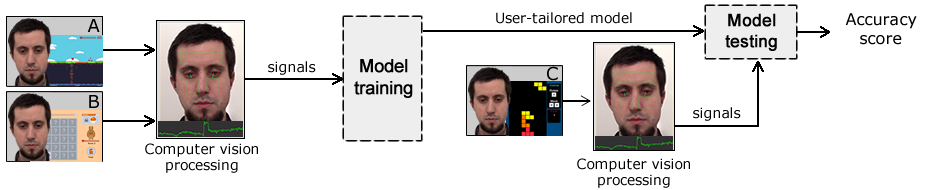
\includegraphics[width=\textwidth]{Content/figures/machine-learning-investigation.png}
    \caption{Iteration of a 3-fold \textit{Leave-One-Session-Out Cross-Validation} performed on the gaming session of a given subject with 3 games, i.e. A, B and C. Data of two calibration games, e.g. A and B, are used to train the machine learning model, while data of the third calibration game, e.g. C, is used to evaluate the model.}
    \label{fig:study5-training-evaluation}
\end{figure}

\textit{Leave-One-Session-Out Cross-Validation} (LOSOCV) is used to evaluate each trained user-tailored model, as illustrated in Figure \ref{fig:study5-training-evaluation}. In LOSOCV, data from one session instance is left out and a model is constructed on data from all other session instances. In the present study, a given subject $S_i$ played 3 calibration games, e.g. A, B and C, so data from one calibration game is left out and a model is trained on the data of the other two calibration games for that subject $S_i$. This is repeated for all three calibration games of that subject $S_i$. Consequentially the use of LOSOCV will produce 3 models per subject, resulting in 3 measurements of classificaiton accuracy per subject, denoted $L_j$, where $j \in \{1, 2, 3\}$ represent each evaluated model. The final classification accuracy for given subject $S_i$, named $A_i$, is calculated as the mean of $L_j$ values obtained from the iterations in the LOSOCV. In other words, each subject contributes a single classification accuracy value $A_i$, which is calculated based on the mean classification accuracy of his/her three models in the LOSOCV iterations.

In the training process of each model, which is performed 3 times per user, the hyper-parameters of each neural network, e.g. number of neurons, is optimized using random search \parencite{bergstra2012random}. A 10-fold cross validation method repeated 3 times is applied, so the dataset is split into 10-subsets and each of those subset is held out while the model is trained on all others. The process is repeated 3 times and the final metric for the model is the mean from the number of repeats. Area under the ROC curve (AUC) is used as a metric to select the best model.

According to previous analysis, subjects perceived the games as being boring at the beginning and stressful at the end. As a consequence, it is assumed that subject's emotional state in $H_0$ and $H_1$ is boredom and stress, respectively. Based on that assumption, training and evaluation data obtained from video segments in $H_0$ and $H_1$ were labeld as boredom and stress, respectively.

%, which finds models as good or beter then ones configured by a pure grid search

%Describe how the model was trained, which includes how the calibration games were grouped, e.g. two for training, one for testing. Explain that neural networks were used because they are widely mentioned in the literature.

%%%%%%%%%%%%%%%%%%%%%%%%%%%%%%%%%%%%%%%%%%%%%%%%%%%%%%%%%%%%%%%%%%%%%%%%
\subsubsection{Analysis}
\label{sec:experiment1-study5-analysis}
%%%%%%%%%%%%%%%%%%%%%%%%%%%%%%%%%%%%%%%%%%%%%%%%%%%%%%%%%%%%%%%%%%%%%%%%%

In order to test the effectiveness of the neural network in classifying samples as either boredom or stress, all trained neural networks were evaluated in conjunction. As described in the previous section, each subject's model was evaluated using LOSOCV, which produced a classification accuracy $A_i$ for any given subject $S_i$. The minimum, maximum and mean value of $A_i$ was calculated as a metric for accuracy. In order to better contextualize the classification results, the same process was also applied to other three metrics obtained during the LOSOCV evaluation: Precision, Recall and F1 score\footnote{F1 score should not be confused with $F_1$, the mouth outer facial feature used in the model.}. Precision accounts for the correctly predicted positive observations over the total of predicted positive observations, e.g. from all samples classified as stress, how many of those were indeed labeled as stress. Recall accounts for the correctly predicted positive observations over all available observations in a class, e.g. from all available samples labeled as boredom (or stress), how many were actually classified as such. Finally F1 score is the weighted average of Precision and Recall.

Aiming to better understand the contribution of each feature for the classification process, the training/evaluation process mentioned early was also performed using different feature sets. Each of those different feature sets was evaluated in an independent test, denoted $T_i$. Table \ref{table:study5-different-feature-sets} shows tests $T_i$ and the corresponding feature sets used in the process.

\begin{table*}
    \centering
    \caption{Tests and their respective feature sets}
    \label{table:study5-different-feature-sets}
    \begin{tabular}[l]{@{}cclp{4.0cm}}
        \toprule%
            \textbf{$T_i$} & \textbf{Name} & \textbf{Feature set} & \textbf{Note} \\
        \midrule%
            1 & \texttt{MULTI\_R} & $F_1^\mu$, $F_2^\mu$, $F_3^\sigma$, $F_4^\sigma$, $F_5^\mu$, $F_6^\sigma$, $F_8$ & Facial analysis, rPPG-estimated HR.\\ % 5278d175-71e752ce: HR_poh2011, mean_face_activity_mouth_corner, mean_face_activity_mouth_outer, mean_face_area, std_face_activity_eyebrow, std_face_eye_area, std_face_motion_instability
            2 & \texttt{MULTI\_G} & $F_1^\mu$, $F_2^\mu$, $F_3^\sigma$, $F_4^\sigma$, $F_5^\mu$, $F_6^\sigma$, $F_9^\mu$ & Facial analysis, HR from physical sensor.\\ % 5278d175-9fa716ee: mean_HR_ground, mean_face_activity_mouth_corner, mean_face_activity_mouth_outer, mean_face_area, std_face_activity_eyebrow, std_face_eye_area, std_face_motion_instability
            3 & \texttt{FACE} & $F_1^\mu$, $F_2^\mu$, $F_3^\sigma$, $F_4^\sigma$, $F_5^\mu$, $F_6^\sigma$ & Facial analysis only. \\ % 5278d175-826512b2: mean_face_activity_mouth_corner, mean_face_activity_mouth_outer, mean_face_area, std_face_activity_eyebrow, std_face_eye_area, std_face_motion_instability
            4 & \texttt{HR\_R} & $F_8$ & rPPG-estimated HR only.\\ % 5278d175-97a38001: HR_poh2011
            5 & \texttt{HR\_G} & $F_9^\mu$ & HR from physical sensor only. \\ % 5278d175-ad2580a5: mean_HR_ground
        \bottomrule%
    \end{tabular}
\end{table*}

Tests \texttt{MULTI\_R} and \texttt{MULTI\_G} use multifactorial set of features for their neural network, where facial and HR information are used in combination. The difference between \texttt{MULTI\_R} and \texttt{MULTI\_G} is that the former uses rPPG estimated HR, while the latter uses HR obtained from the physical sensor. Test \texttt{FACE} uses a set of features based solely on facial information. Finally tests \texttt{HR\_R} and \texttt{HR\_G} use only HR information as a feature. Similarly to \texttt{MULTI\_R} and \texttt{MULTI\_G}, tests \texttt{HR\_R} and \texttt{HR\_G} use HR readings from rPPG estimatations and from a physical sensor, respectively.

Subjects perceived the games as boring and stressful, so such difference should make a trained neural network capable of properly classifying evaluation samples as either boredom or stress. Additionally the use of a multifactorial approach, where facial analysis and HR information are used in combination instead of either one alone, is expected to produce better classification results \parencite{zacharatos2014automatic}. Based on those expectations, the following hypotheses are stated:

\begin{itemize}
  \item $u_1$: a user-tailored neural network trained on data samples from two calibration games of a given subject $S_i$ is able to classify samples from a third calibration game of that same subject $S_i$ with an accuracy greater than chance-level rate (random guessing);
  \item $u_2$: a user-tailored neural network using a multifactorial feature set, i.e. facial and HR features, performs with greater accuracy than a user-tailored neural network using facial features only;
  \item $u_3$: a user-tailored neural network using a multifactorial feature set, i.e. facial and HR features, performs with greater accuracy than a user-tailored neural network using HR features only.
\end{itemize}

Hypothesis $u_1$ was tested by checking if the mean value of the classification accuracy, i.e. calculated from all $A_i$ values, is greater than 0.5. In such case it is assumed that an accuracy rate of 0.5 (50\%) is the theoretical probabilistic chance level achieved by totally random classification performed by a classifier evaluated on an infinite number of data samples. Hypotheses $u_2$ and $u_3$ were tested by performing a Wilcoxon Signed Ranks test on all $J_i$ values of the two competing tests $T_i$. As previously mentioned, the use of LOSOCV produces 57 accuracy measuraments $J_i$ per test $T_i$.

%%%%%%%%%%%%%%%%%%%%%%%%%%%%%%%%%%%%%%%%%%%%%%%%%%%%%%%%%%%%%%%%%%%%%%%%%
\subsection{Results}
%%%%%%%%%%%%%%%%%%%%%%%%%%%%%%%%%%%%%%%%%%%%%%%%%%%%%%%%%%%%%%%%%%%%%%%%%

Table \ref{table:study5-result-metrics-mean} presents the mean values of the resulting classification metrics for accuracy, precision, recall and F1 score, calculated and analyzed according to the procedures described in Section \ref{sec:experiment1-study5-method}. Regarding the accuracy metric, the highest mean value achieved was 62.3\% in test \texttt{MULTI\_G}, whose model used a combination of facial and HR features. The HR feature in that case was calculated from the physical sensor, not remotely estimated. The second and third highest accuracy rates were 60.8\% in test \texttt{HR\_G} (HR from physical sensor only) and 60.4\% in test \texttt{MULTI\_R} (facial and remotely-estimared HR features), respectively. The highest values achieved for precision, recall and F1 score were 65.6\%, 62.4\%, and 58.1\%, respectively, all in test \texttt{HR\_G}.

\begin{table*}
    \centering
    \caption{Mean values of resulting classification metrics}
    \label{table:study5-result-metrics-mean}
    \begin{tabular}[l]{@{}ccccc}
        \toprule%
            \textbf{Test} & \textbf{Accuracy} & \textbf{Precision} & \textbf{Recall} & \textbf{F1}\\
        \midrule%
            \texttt{MULTI\_R} & 0.604 & 0.612 & 0.599 & 0.521 \\ % 5278d175-71e752ce
            \texttt{MULTI\_G} & \textbf{0.623} & 0.583 & 0.607 & 0.514 \\ % 5278d175-9fa716ee
            \texttt{FACE} & 0.594 & 0.601 & 0.585 & 0.507 \\ % 5278d175-826512b2
            \texttt{HR\_R} & 0.547 & 0.541 & 0.545 & 0.497 \\ % 5278d175-97a38001
            \texttt{HR\_G} & 0.608 & \textbf{0.656} & \textbf{0.624} & \textbf{0.581} \\ % 5278d175-ad2580a5
        \bottomrule%
    \end{tabular}
\end{table*}

Table \ref{table:study5-result-metrics-minmax} presents a discrimination of the minumum and maximum mean values for the resulting classification metrics. At least one subject in test \texttt{MULTI\_G} has been classified with a mean accuracy of 98\%, the highest value for that metric in all tests. The worst mean accuracy value was 19\% for at least one subject in test \texttt{MULTI\_R}. Regarding precision, the highest mean value was 97\% in test \texttt{MULTI\_G}. In all tests but \texttt{HR\_G}, at least one subject has been classified with zero precision (all samples were classified wrongly). Regarding precision, the highest and lowest mean values were 98\% and 12\% in tests \texttt{MULTI\_G} and \texttt{FACE}, respectively. Finally regarding F1 score, the highest mean value was 98\% for at least one subject in test \texttt{MULTI\_G}. All tests presented zero as the lowest F1 score.

\begin{table}[!htbp]
  \centering
  \caption{Minimum and maximum mean values of resulting classification metrics}
  \label{table:study5-result-metrics-minmax}
  \begin{tabular}{ccccccccc}
    \toprule%
      \textbf{Test} & \multicolumn{2}{c}{\textbf{Accuracy}} & \multicolumn{2}{c}{\textbf{Precision}} & \multicolumn{2}{c}{\textbf{Recall}} & \multicolumn{2}{c}{\textbf{F1}} \\
      {} & min & max & min & max & min & max & min & max \\
    \midrule%
      \texttt{MULTI\_R}  & 0.19 & 0.91 & 0.00 & 0.95 & 0.19 & 0.87 & 0.00 & 0.91 \\ % 5278d175-71e752ce
      \texttt{MULTI\_G}  & 0.25 & \textbf{0.98} & 0.00 & \textbf{0.97} & 0.13 & \textbf{0.98} & 0.00 & \textbf{0.98} \\ % 5278d175-9fa716ee
      \texttt{FACE}  & 0.26 & 0.90 & 0.00 & 0.95 & 0.12 & 0.90 & 0.00 & 0.89 \\ % 5278d175-826512b2
      \texttt{HR\_R}  & 0.36 & 0.72 & 0.00 & 0.79 & 0.18 & 0.77 & 0.00 & 0.67 \\ % 5278d175-97a38001
      \texttt{HR\_G}  & 0.38 & 0.82 & 0.26 & 0.85 & 0.23 & 0.87 & 0.00 & 0.81 \\ % 5278d175-ad2580a5
    \bottomrule%
  \end{tabular}
\end{table}

% data_multi_r and data_hr_r: p = 0.04488, Zstat = -2.0058, effect = 0.2657
% data_multi_r and data_face: p = 0.26797, Zstat = -1.1077, effect = 0.1467

Finally there are indications that a multifactorial model, which uses a combination of facial and HR features, performs with greater accuracy than a model using either facial or HR features. A Wilcoxon Signed Ranks test indicates that the mean accuracy was greater for a multifactorial model using facial and remotely estimated HR features, i.e. \texttt{MULTI\_R}, than for a model using only remotely estimated HR, i.e. \texttt{HR\_R}, $Z=-2.00$, $p=0.044$, $r=0.26$. However there are no indications that the mean accuracy of such multifactorial model, i.e. \texttt{MULTI\_R}, is statistically significantly greater than the mean accuracy of a model using only facial features, i.e. \texttt{FACE}, $Z=-1.10$, $p=0.267$, $r=0.14$.

%%%%%%%%%%%%%%%%%%%%%%%%%%%%%%%%%%%%%%%%%%%%%%%%%%%%%%%%%%%%%%%%%%%%%%%%%
\subsection{Discussion}
%%%%%%%%%%%%%%%%%%%%%%%%%%%%%%%%%%%%%%%%%%%%%%%%%%%%%%%%%%%%%%%%%%%%%%%%%

% data_multi_g and data_face: p = 0.03343, Zstat = -2.1269, effect = 0.2817
% data_multi_g and data_hr_g: p = 0.27802, Zstat = -1.0848, effect = 0.1437

% data_multi_g and data_multi_r: p = 0.07836, Zstat = -1.7603, effect = 0.2332

Results indicate that the use of a user-tailored model to remotely estimate the emotional state of players from videos of gaming sessions is feasible. Previously mentioned hypothesis $u_1$ states that a user-tailored neural network trained on data samples from two calibration games of a given subject $S_i$ is able to classify samples from a third calibration game of that same subject $S_i$ with an accuracy greater than chance-level rate (random guessing). Such model was tested in two configurations: \texttt{MULTI\_R} and \texttt{MULTI\_G}. Model \texttt{MULTI\_R}, which uses a multifactorial feature set composed of facial and remotely estimated HR information, presented a mean classification accuracy of 60.4\%. Such reported accuracy is greater than 50\%, the theoretical probabilistic chance level, which confirms hypothesis $u_1$. Model \texttt{MULTI\_G}, which also uses a multifactorial feature set but differs in the acquisition of HR data, i.e. physical sensor instead of remote estimation, presented a mean classification accuracy of 62.3\%. Such reported accuracy is also greater than the theoretical probabilistic chance level. The slightly greater classification accuracy of model \texttt{MULTI\_G} compared to \texttt{MULTI\_R} suggests that more precise rPPG estimations of the HR could improve the overall classification accuracy of model \texttt{MULTI\_R}. A Wilcoxon Signed Ranks test, however, has no statistically significant indication that the accuracy was greater for \texttt{MULTI\_G} than for \texttt{MULTI\_R}, $Z=-1.76$, $p=0.078$, $r=0.23$. Despite not being statistically significant, values $p=0.078$ and $r=0.23$ (small effect according to Cohen's classification of effect size) suggest a trend towards that reasoning.

Hypothesis $u_2$ states that a user-tailored neural network using a multifactorial feature set performs with greater accuracy than a user-tailored neural network using facial features only. The Wilcoxon Signed Ranks test mentioned in the previous section presented no statistically significant indications that the classification accuracy of \texttt{MULTI\_R} is greater than \texttt{FACE}. It is possible to speculate that a set of facial features, e.g. eyebrow and mouth analysis, has a greater potential to differentiate emotional states in a classifier. Particularly it might perform better than a classifier based on rPPG-estimated HR alone.

Regarding hypothesis $u_3$, which states that a user-tailored neural network using a multifactorial feature set performs with greater accuracy than a user-tailored neural network using HR features only. The Wilcoxon Signed Ranks test mentioned in the previous section presents statistically significant indications that the classification accuracy of \texttt{MULTI\_R} is greater than \texttt{HR\_R}. It supports the claim of hypothesis $u_3$, confirming that a multifactorial model performs better than one based solely on remotely estimated HR data. The lower classification potential of remotely estimated HR, however, could be attributed to errors in the rPPG estimation process caused by noise, e.g. natural movement of subjects (see Section \ref{sec:experiment1-study3}, on page \pageref{sec:experiment1-study3}, for more information). As a consequence, a more precise HR estimation used in a multifactorial model allegedly contributes to produce a better classifier. A Wilcoxon Signed Ranks test confirms with statistical significance that the classification accuracy of \texttt{MULTI\_G}, i.e. facial and HR from sensor, is greater than the accuracy of \texttt{FACE}, i.e. facial information only, $Z=-2.12$, $p=0.033$, $r=0.28$. It supports the previously mentioned idea that a precise HR estimation (from a physical sensor in the case of \texttt{MULTI\_G}) combined with facial information is a better classifier than one using facial information alone, i.e. model \texttt{FACE}. Finally a Wilcoxon Signed Ranks test does not indicate that the accuracy of \texttt{MULTI\_G} is greater than \texttt{HR\_G}, $Z=-1.08$, $p=0.278$, $r=0.14$. Consequentially it seems that precise estimations of HR is important, but HR or facial information used separately are likely to be less important for classification then a joint, multifactorial use of them in the emotion classification process.

Finally it is important to highlight the possible limitations of using the theoretical probabilistic chance level rate of 50\% for the evaluation of the model's accuracy. As previously mentioned, an accuracy baseline of 50\% assumes a totally random classification evaluated on an infinite number of data samples. One could argue that such scenario is unrealistic. In that case, the true evaluation of a model must consider statistical significance levels taking into account the sample size used in the process. \textcite{combrisson2015exceeding} present a work in the field of brain signal classification that uses analytical and empirical solutions, i.e. binomial formula and permutation tests, to show the influence of small numbers of data samples in the theoretical probabilistic chance level. According to the authors, a minimal correct classification rate of 62.5\% is required to assert statistical significance, i.e. $p < 0.05$, during the classification of two classes with a sample size of 40. In the present study, each subject was evaluated with 38 samples on average\footnote{This number refers to the amount of samples used for the evaluation of a model, not its training. During the training phase of each model, more than 38 samples were used per subject.}. As presented in the results of this study, the mean accuracy rate of models \texttt{MULTI\_R} and \texttt{MULTI\_G} are 60.4\% and 62.3\%, respectively. Following the analysis of \textcite{combrisson2015exceeding}, the mean accuracy rate of those multifactorial models would not be enough to assert statistical significance of the results. Nevertheless both models presented a mean accuracy that trends towards the minimal 62.5\%. Additionally the previously mentioned Wilcoxon Signed Ranks test does not indicate that the accuracy was greater for \texttt{MULTI\_G} than for \texttt{MULTI\_R}, so their performance could be the same. It is also important to stress the use of Leave One Session Out Cross Validation in the evaluation of each subject. It uses a completely independent and different game as source of sampling for the evaluation of each model, which strengthens the evaluation process. The reduced number of subjects in the study, i.e. 19, and the reduced number of samples used in the evaluation of each models, i.e. 38 on average, are in fact limiting factors. Reported results, however, provide insights regarding the feasibility of a multifactorial remote approach for emotion classification. The accuracy of the models presented in this study are not statistically confirmed without the assumption of baseline produced by a random classifier evaluated on an infinite number of data samples. However there is in fact a trend indicating that the use of a user-tailored model to remotely estimate emotional states of players is worth of further investigation.

% From: https://www.sciencedirect.com/science/article/pii/S1053811916000604#bb0235
% Recently, Combrisson and Jerbi (2015) compared the various statistical tests used to evaluate decoding performance and showed that the theoretical chance level was less stringent for small numbers of data samples, as found in neuroimaging studies, causing a bias towards statistical significance. The permutation test, by contrast, is not open to this criticism because it is a data-driven method and does not make assumptions about the statistical properties of the dataset. Therefore, the significance test we used may have been more stringent than the one used by those obtaining positive decoding findings in FFA.

%%%%%%%%%%%%%%%%%%%%%%%%%%%%%%%%%%%%%%%%%%%%%%%%%%%%%%%%%%%%%%%%%%%%%%%%%
\subsection{Conclusions}
%%%%%%%%%%%%%%%%%%%%%%%%%%%%%%%%%%%%%%%%%%%%%%%%%%%%%%%%%%%%%%%%%%%%%%%%%

This study presented a systematic evaluation of the feasibility of using a user-tailored neural network trained on data samples from two calibration games of a given subject to classify emotional states from a third calibration game of that same subject. Further investigation is required, however results suggest that a user-tailored neural network, based on remotely acquired data from video recordings, is able to classify emotional states with an accuracy greater than chance-level rate (random guessing).

Regarding the efficiency of a multifactorial model, where facial and HR information are together instead of separately, there are no statistically significant indications that the classification accuracy of such a model is greater than a model using facial information alone. However a multifactorial model based on remotely acquired data performs better than one based solely on remotely estimated HR data.

Finally it seems that precise estimations of HR is important, but HR or facial information used separately are likely to be less important for classification than a combined use of them in a multifactorial emotion classification model based on remotely acquired data. The analysis performed in this study supports further investigation regarding a user-tailored model to remotely estimate emotional states of player.


\chapter{Experiment 2: validation of remote detection of emotions}
\label{ch:experiment2}

The experiment described in this chapter, the second conducted, aimed at validating the proposed approach for the remote detection of emotions, described in the objectives of this thesis (Section \ref{sec:contributions}, page \pageref{sec:contributions}). The approach uses remotely acquired signals, namely, heart rate (HR) and facial actions (FA), to create a user-tailored model, i.e. trained neural network, that is able to detect the emotional states of boredom and stress of a given subject. The approach is composed of two phases: training (or calibration) and testing. In the training phase, the model is trained by applying a user-tailored approach, i.e. data from subject $S_a$ playing 3 calibration games (Mushroom, Platformer and Tetris) are used to create model $N_a$. The result of the training phase is a user-tailored model, i.e. model $N_a$, a trained neural network for use on subject $S_a$. The testing phase occurs in a game session involving subject $S_a$ playing any ordinary, non-calibration game, e.g. COTS game. During the testing phase, the signals of subject $S_a$ are remotely acquired and fed into the previously trained model $N_a$, which outputs the estimated emotional state of subject $S_a$ for that particular testing game.

In summary, the aim of this experiment was to answer the following research question:

\begin{fquote}
How accurate is an emotion detection approach that uses remotely acquired signals, i.e. heart rate and facial actions, as input of a machine learning model, i.e. neural network, that is trained on a user-tailored basis (one subject produces one model) using calibration games as emotion elicitation?
\end{fquote}

The overall goal of this experiment is to validate the proposed approach and prove its feasibility by analyzing the emotion classification accuracy during the testing phase. The following sections present a detailed explanation of the experiment, including its participants, structure and results, as well as a discussion and a conclusion.

%%%%%%%%%%%%%%%%%%%%%%%%%%%%%%%%%%%%%%%%%%%%%%%%%%%%%%%%%%%%%%%%%%%%%%%%%%%%%%%%%%%%%%%
\section{Participants}
%%%%%%%%%%%%%%%%%%%%%%%%%%%%%%%%%%%%%%%%%%%%%%%%%%%%%%%%%%%%%%%%%%%%%%%%%%%%%%%%%%%%%%%

Sixty two ($N=62$) adult participants\footnote{Participants of this experiment (Experiment 2) and those of Experiment 1 (detailed in Chapter \ref{ch:experiment1}, page \pageref{ch:experiment1}) are different. There is no overlap of subjects in both experiments.} of both genders (38.7\% female, 61.3\% male) with different ages (19 to 66, mean 27.2, SD 7.2) and different gaming experience gave their informed and written consent to participate in the experiment. The study population consisted of staff members and students of the University of Sk\"ovde, as well as inhabitants of the community/city.

In response to the question regarding the participants' level of skill playing video games, 6 (9.7\%) reported no skill, 19 (30.6\%) reported not very skilled, 25 (40.3\%) reported moderately skilled and 12 (19.9\%) reported very skilled. In response to the question regarding the number of hours per week playing any type of video game over the last year, 25 (40.3\%) reported more than 10, 7 (11.3\%) reported 5 to 10, 6 (9.7\%) reported 3 to 4, 5 (8.1\%) reported 1 to 3, 10 (16.1\%) reported 0 to 1, and 9 (14.5\%) reported no activity.

These numbers indicate that the sample population has a diversity of ages, gaming experience and playing frequency. Such diversity provides heterogeneous data that allow a more realistic and broad analysis of the proposed method.

%%%%%%%%%%%%%%%%%%%%%%%%%%%%%%%%%%%%%%%%%%%%%%%%%%%%%%%%%%%%%%%%%%%%%%%%%%%%%%%%%%%%%%%
\section{Method}
\label{sec:experiment2-method}
%%%%%%%%%%%%%%%%%%%%%%%%%%%%%%%%%%%%%%%%%%%%%%%%%%%%%%%%%%%%%%%%%%%%%%%%%%%%%%%%%%%%%%%

The following sections present the experiment structure and the methods employed to collect and analyze data.

%%%%%%%%%%%%%%%%%%%%%%%%%%%%%%%%%%%%%%%%%%%%%%%%%%%%%%%%%%%%%%%%%%%%%%%%%%%%%%%%%%%%%%%
\subsection{Experimental design and setup}

Subjects were seated alone in the room, in front a computer, while recorded by a camera and measured by a heart rate sensor, as illustrated in Figure \ref{fig:experiment2-setup}. The camera was attached to a tripod and placed in front of the subjects at a distance of approximately 0.6m; the camera was tilted slightly up. A spotlight, tilted 45$^{\circ}$ up, placed at a distance of 1.6m from the subject and 45cm higher than the camera level, was used for illumination; no other light source was active during the experiment.

\begin{figure}[ht]
\centering
  \begin{subfigure}[b]{0.5\textwidth}
    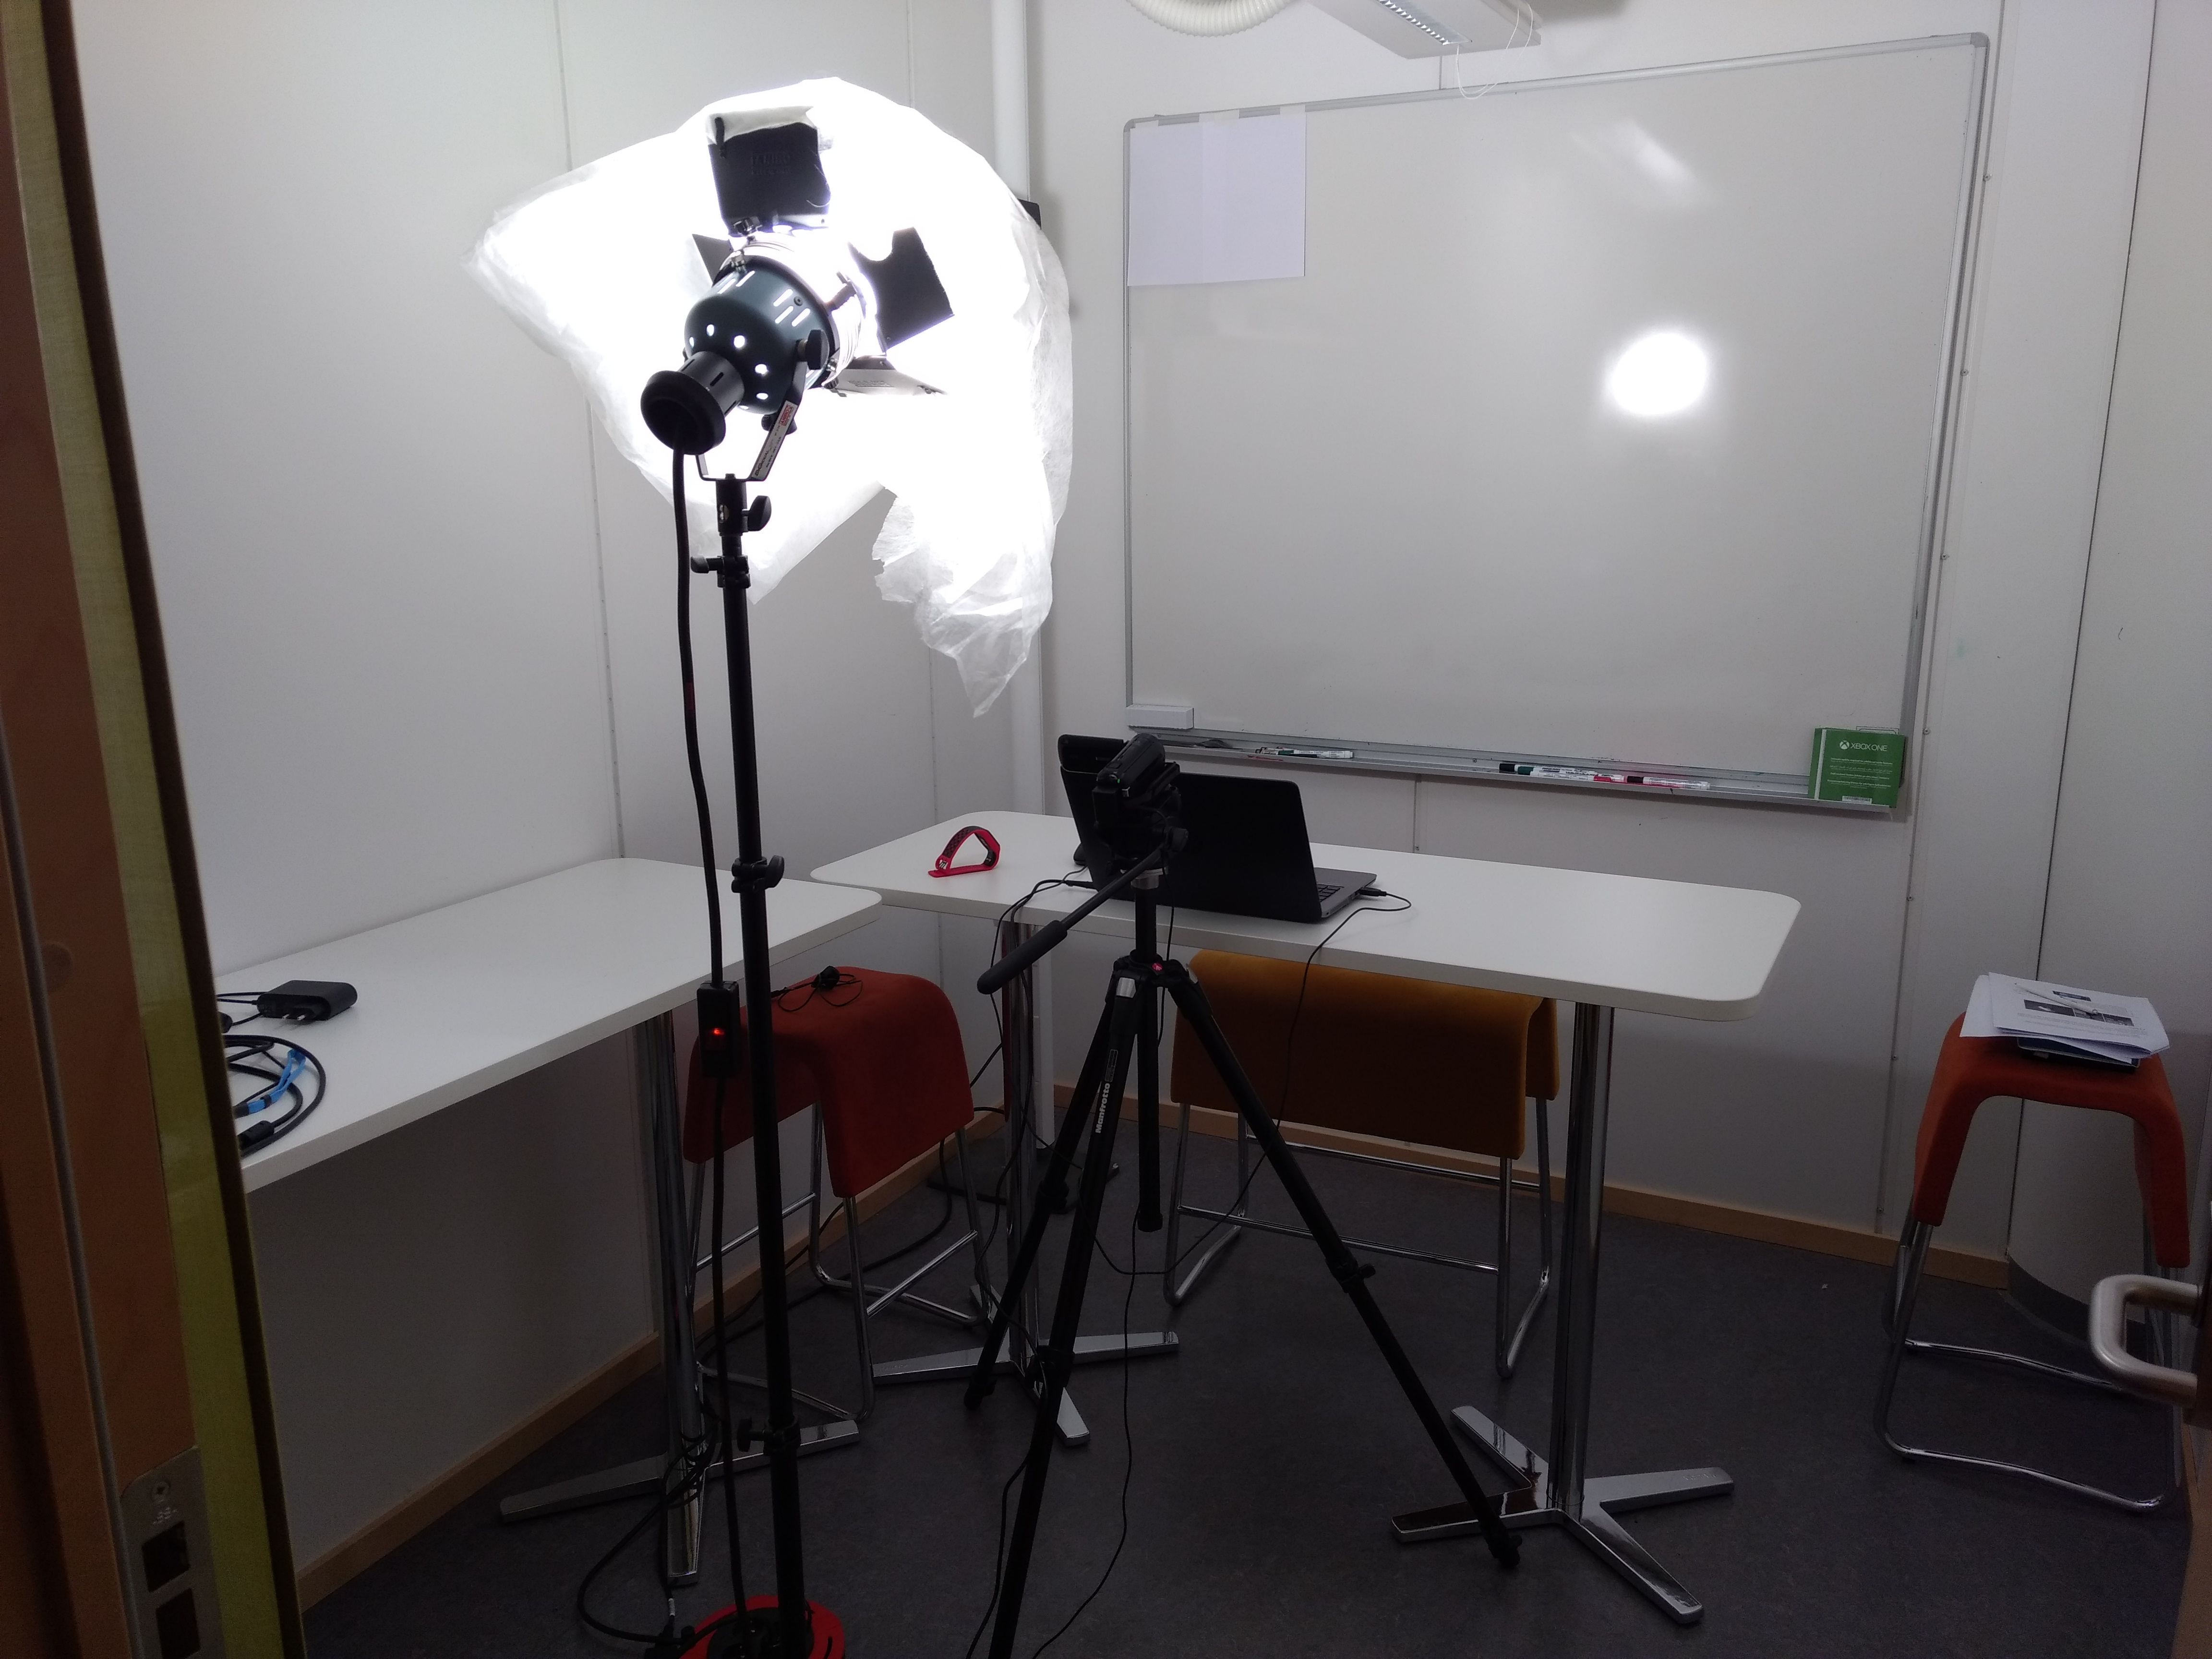
\includegraphics[width=0.95\textwidth]{Content/figures/experiment2-setup-overall}
    \caption{}
    \label{fig:experiment2-setup-overall}
  \end{subfigure}%
  \begin{subfigure}[b]{0.5\textwidth}
    \centering
    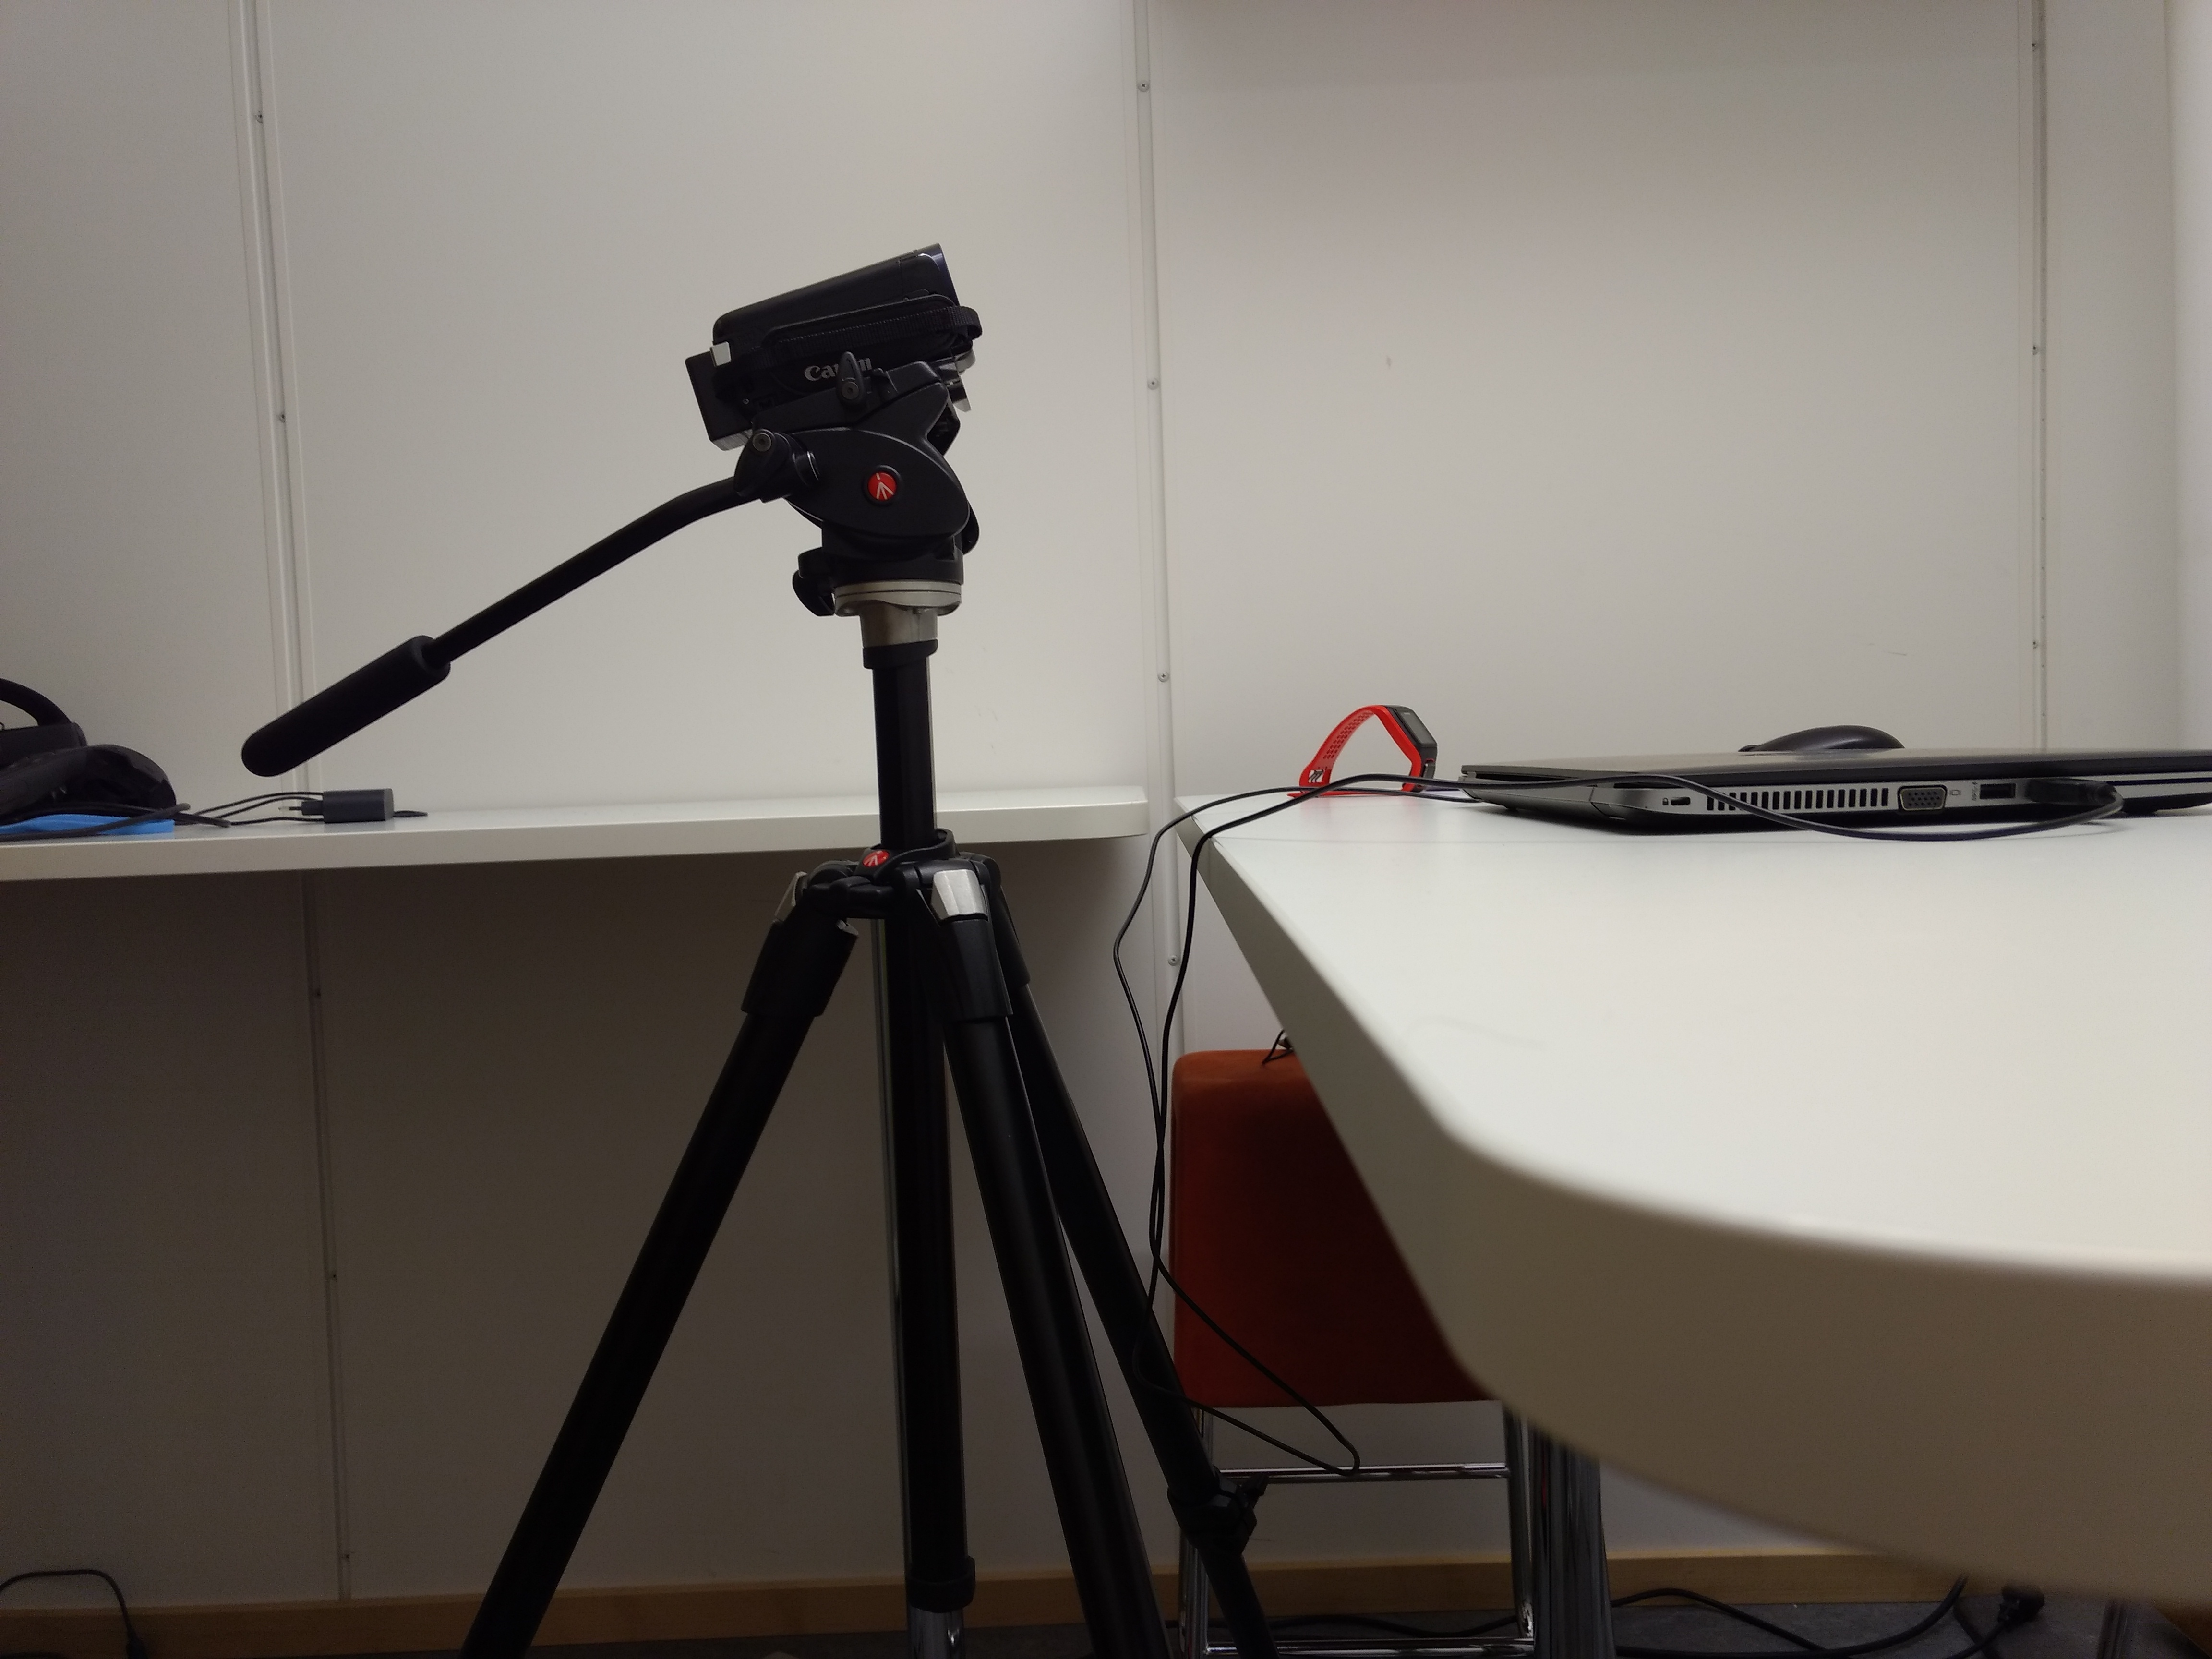
\includegraphics[width=0.95\textwidth]{Content/figures/experiment2-setup-camera}
    \caption{}
    \label{fig:experiment2-setup-camera}
  \end{subfigure}
  \caption{Experiment setup. (a) Position of equipment, showing computer, camera, and external light source. (b) Highlight of the video camera and its angle.}
  \label{fig:experiment2-setup}
\end{figure}

Each participant was recorded for an average of 45 minutes during two (uninterrupted) parts of the experiment, i.e. the calibration and testing phase, as illustrated by Figure \ref{fig:experiment2-parts}. In the calibration part, aimed at gathering data for training a user-tailored model, the subjects played 3 calibration games (described in Section \ref{sec:experiment2-calibration-games}). Each of these games was followed by a questionnaire related to the game and the stress/boredom levels. The games were also followed by a rest period of 138 seconds during which the subjects listened to calm classic music. In the testing part, aimed at gathering data to test the accuracy of the user-tailored model, the subjects played 7 levels of an evaluation game, i.e. Infinite Mario (described in Section \ref{sec:experiment2-evaluation-game}). In the calibration phase of the experiment, the order in which the games were played was randomized among the subjects.

%In the calibration part, games were carefully designed to start with a difficulty level that is significantly low, which is expected to lead the player to an immediate state of boredom. As time progresses, the difficulty level increases linearly. As the difficulty level continues to rise, at certain point the game becomes too hard to be managed by the subject, which eventually results in a ``game over" state. Moments before that point the subject should reach his/her stress peak during gameplay. It is expected that each player experiences three distinct states during the gameplay of each game: boredom (low challenge, low stress) at the beginning, flow (ideal challenge/stress) after the beginning and before the final moments, and stress (high challenge, high stress) at the end. The order in which the games were played was randomized among subjects during the calibration phase of the experiment.

\begin{figure}[ht]
  \centering
  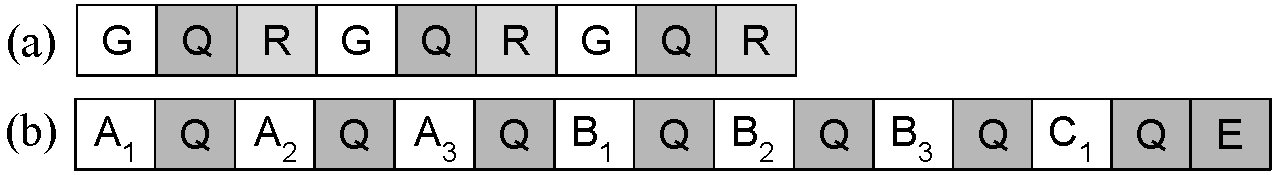
\includegraphics[width=0.95\textwidth]{Content/figures/experiment2-parts}
  \caption{Two (uninterrupted) parts of the experiment. (a) Calibration part; (b) Testing part. G: calibration game, Q: questionnaire about game/level, R: resting, ABC: levels of Infinite Mario, E: demographic questionnaire.}
  \label{fig:experiment2-parts}
\end{figure}

In the testing part, the subjects played 3 batches of Infinite Mario levels: batches $A$, $B$ and $C$ containing 3, 3 and 1 level each, respectively. The levels in batches $A$ and $B$ were designed to present an increase in difficulty within the batch; therefore, levels $A_1$ and $B_1$ were expected to be less difficult/challenging than levels $A_3$ and $B_3$, for instance. Similarly, the levels in batch $B$ were designed to be more challenging than the levels in batch $A$, also following an increase in difficulty. Consequently, levels $B_i$ are expected to be slightly more difficult/challenging than levels $A_i$. This pattern intended to mimic the balance curve of a commercial game, where levels, and game parts, commonly tend to increase their difficulty as the game story progresses. In order to ensure that the subjects would experience some level of boredom during the testing phase, which is required for the evaluation of the proposed method, levels $B_1$ and $C_1$ were designed using a particular set of changes, including the use of Mario's auto-scrolling camera mechanics. In such a configuration, the player has no control of the speed of the level. After each level was played, the subjects were required to answer a questionnaire about how boring/stressful the game level had been. The order in which the levels were played was not randomized among the subjects during the testing phase of the experiment. As a consequence, all the subjects played the evaluation game in the same order: levels $A_1$ to $A_3$, then by levels $B_1$ to $B_3$, finally level $C_1$.

%This mechanic is expected to induce boredom, since the player experienced allegedly challenging (and fun) levels previously and is now unable to move using any desired speed

After the subjects finished playing the last level in the testing part, i.e. level $C_1$, they answered a final questionnaire about their age and gaming experience/profile. Before starting the experiment, the participants received the following instructions from a researcher: they should play a few games, answer questionnaires after each game and rest when instructed; they were told that their gaming performance was not being evaluated, that they should not give up in the middle of the games, that a time limit exists for some levels to prevent them from playing too long, and that they should remain seated during the whole process.

\subsection{Calibration games}
\label{sec:experiment2-calibration-games}

The three calibration games, i.e. Mushroom, Platformer and Tetris, have already been described in detail in Section \ref{sec:experiment1-games-elicitation} (page \pageref{sec:experiment1-games-elicitation}). The present experiment used exactly the same calibration games as in the first experiment (see Chapter \ref{ch:experiment1}). The games are 2D, casual-themed, and played with mouse or keyboard in a web browser. They were carefully designed to provoke boredom at the beginning and stress at the end, with a linear progression between the two states.

\subsection{Evaluation game}
\label{sec:experiment2-evaluation-game}

%Pedersen, C.; Togelius, J. & Yannakakis, G. N. Modeling player experience in Super Mario Bros. 2009 IEEE Symposium on Computational Intelligence and Games, IEEE, 2009, 132-139

%Pedersen, Christopher, Julian Togelius, and Georgios N. Yannakakis. "Modeling player experience for content creation." IEEE Transactions on Computational Intelligence and AI in Games 2.1 (2010): 54-67.

%Shaker, N.; Asteriadis, S.; Yannakakis, G. N. & Karpouzis, K. A game-based corpus for analysing the interplay between game context and player experience. Affective Computing and Intelligent Interaction, Springer, 2011, 547-556

% Shaker, N.; Yannakakis, G. N. & Togelius, J. Feature analysis for modeling game content quality. 2011 IEEE Conference on Computational Intelligence and Games (CIG'11), IEEE, 2011, 126-133

The game used in the evaluation phase of the experiment is a modified version\footnote{The version of the game used in the experiment is a HTML5, web-based version built by Robert Kleffner, available at: https://github.com/robertkleffner/mariohtml5. Robert ported to HTML5 the original Java version created by Markus Persson. Source code of both versions, Robert's and Markus', are in the public domain. The source code of the final version used in this experiment is available at: https://fernandobevilacqua.com/link/phd-experiment2} of Markus Persson's Infinite Mario, a public domain clone of Nintendo's platform game \textit{Super Mario Bros}. In the case of this experiment, the game is played with a keyboard in a web browser. Infinite Mario has been widely mentioned in the literature, including studies involving the modeling of player experience \parencite{pedersen2009modeling,pedersen2010modeling,shaker2011game} and detection of affective states \parencite{shaker2011feature}.

\begin{figure}[h]
  \centering
  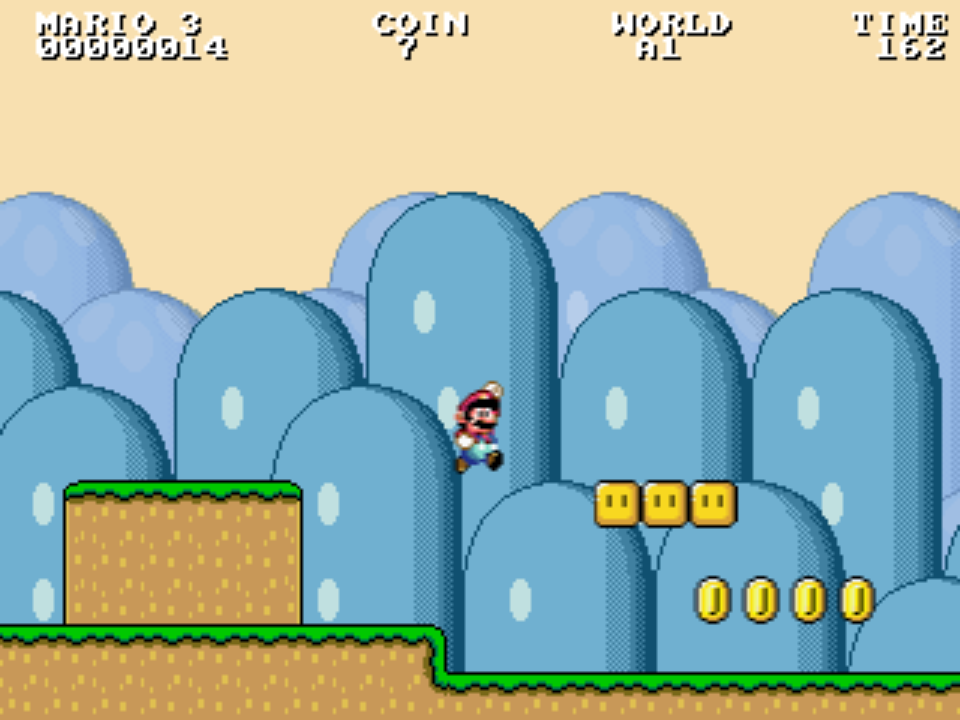
\includegraphics[width=.32\textwidth]{Content/figures/mario-overground}\hfill
  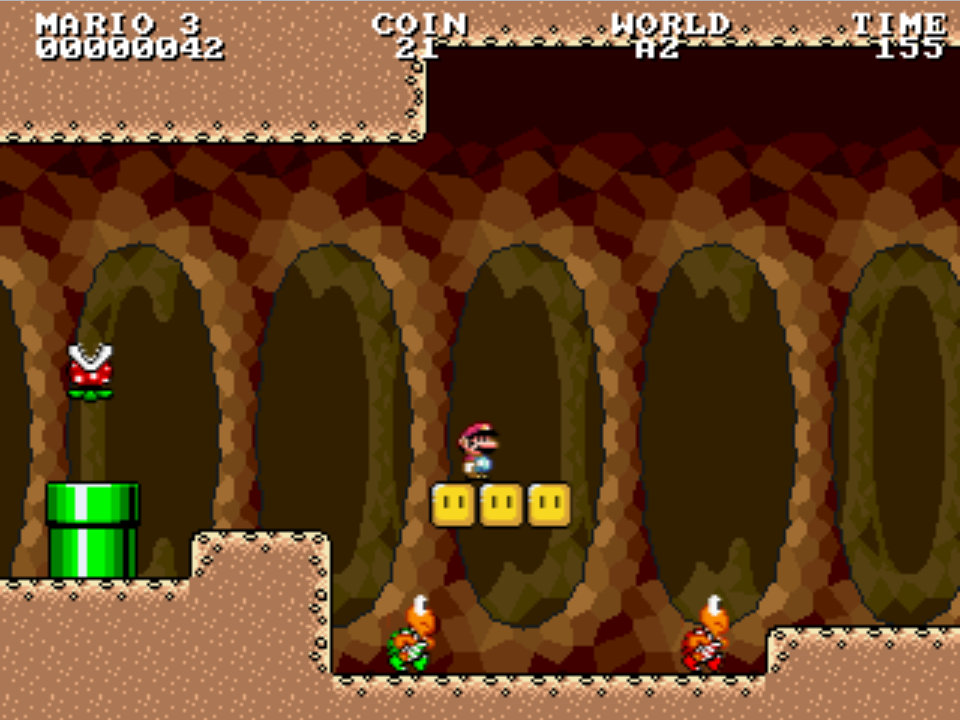
\includegraphics[width=.32\textwidth]{Content/figures/mario-underground}\hfill
  \includegraphics[width=.32\textwidth]{Content/figures/mario-castle}
  \caption{Screenshots from Infinite Mario. From left to right, level types \textit{Overground}, \textit{Underground} and \textit{Castle}, respectively.}
  \label{fig:experiment2-infinite-mario}
\end{figure}

The gameplay in Super Mario, consequentially in Infinite Mario as well, consists of controlling the main character, Mario, along the level. Mario can move left or right, jump, run, duck, and throw fireballs (if the power-up \textit{Flower} has been collected). The objective of the game is to complete each level, which is accomplished by traversing it from left to right until the ``end of level" checkpoint is reached. Mario can be in three different states: small, big, and power-up. If Mario is small, any interaction with enemies that is different from landing on top of them after a jump results in Mario getting killed immediately. If Mario is big, the same ``wrong" interaction with enemies causes Mario to be hurt and transform into the small state. If Mario is in the power-up state, the ``wrong" interaction with enemies causes Mario to be hurt and transform into the big state. Consequently, keeping Mario in the big or power-up state is a strategic advantage that prevents Mario from being killed, which is likely to calm players, i.e. relaxed emotional state. On the other hand, keeping Mario in the small state is less beneficial, since mistakes are fatal, thus likely causing players to feel anxious/stressed in such conditions.

Along the level, Mario might encounter enemies, which can be killed or ignored. Mario can kill enemies by jumping and landing on top of them, which is rewarded with score points. Some enemies, e.g. Koopa Troopa (a sort of turtle), leave a shell behind when killed by Mario. The shell can be picked up by Mario and carried around, serving as a weapon when released. The levels might also contain terrain obstacles of varying sizes, e.g. gaps, that must be jumped over. If Mario falls into a gap, he dies immediately. Mario can also find collectable items, i.e. coins and power-ups, or interactable items, e.g. blocks. Mario collects items by touching them, i.e. a collected coin results in score points. Collectable items might be visible in the level or hidden inside interactable items, e.g. blocks. Mario interacts with blocks by bumping into them from below, e.g. jumping and hitting Mario's head on the bottom of a block destroys it. A destroyed block might give a collectable item as a reward, e.g. coin, \textit{Mushroom} (Mario transitions to big state) or \textit{Flower} (Mario transitions to power-up state).

During gameplay, information about Mario, the score and the current level is displayed at the top of the screen. This information includes the number of lives Mario has left to complete the level, the level score, number of coins collected (collecting 100 coins results in an extra life), name of the current level, and the amount of time available to complete the level (constantly ticking down). When the time remaining to complete the level reaches the 60 seconds mark, a hurry up sound is played, then the background music starts to play in a faster tempo. Unless informed otherwise, all the levels of Infinite Mario in the experiment start with 3 lives and 200 seconds of available time. Every time Mario dies, the time remaining to complete the level is reset to its initial value, e.g. 200 seconds.

Originally, Infinite Mario procedurally generates all its gameplay content, e.g. level design and position of items/enemies. This behavior was not desired for the experiment, since all the subjects should experience the same Mario levels. Additionally, subjects should feel stressed and bored in the game at some points, so that the proposed emotion detection method can be properly evaluated when such moments are detected. As a consequence, Infinite Mario was adapted and tweaked, thus made to fit as an ideal evaluation game in the experiment. The procedural content generation was constrained by a seed and a set of parameters was introduced to control the creation of the content, e.g. length of the level, amount and width of terrain obstacles, such as gaps and platforms, availability of coins and power-ups, among others. It ensured that all the subjects experienced exactly the same levels.

Previous works using Infinite Mario \parencite{pedersen2009modeling,pedersen2010modeling} have shown a correlation between anxiety and 1) difficulty of jumping, e.g. overcoming obstacles, and 2) gap width. There is also a correlation between boredom and the width of gaps, i.e. the wider the gap, the less boring the level. Based on those findings and the guidance provided by game design experts, the Mario levels used in the experiment were adjusted according to the description presented in Table \ref{table:experiment2-mario-levels}. Column \textit{Level} refers to the level name/number. Column \textit{Type} refers to the overall visual representation of the level. Possible types are \textit{Overground} (open sky and green landscape), \textit{Underground} (closed ceiling, dirt-like environment), and \textit{Castle} (closed ceiling with bricks resembling the interior of a castle). Each level type features different background music and visual elements, as illustrated in Figure \ref{fig:experiment2-infinite-mario}. Column \textit{Emotion} refers to the expected emotional state most subjects will experience. Finally, column \textit{Adjustments} refer to the constraints used to generate the levels content.

\begin{landscape}
\begin{table*}
    \centering
    \caption{Levels of Infinite Mario and adjustments made to induce a particular emotional state.}
    \label{table:experiment2-mario-levels}
    \begin{tabular}[l]{@{}cllp{9.5cm}}
        \toprule%
            \textbf{Level} & \textbf{Type} & \textbf{Emotion} & \textbf{Adjustments} \\
        \midrule%
            $A_1$ & Overground  & Any & Reduced number of interactable/collectable items and terrain obstacles; no power-ups; only 2 enemies and 1 gap (with width of Mario himself); Mario starts in big state. \\
            $A_2$ & Underground & Any & Regular number of interactable/collectable items, terrain obstacles, power-ups and enemies. Mario starts in small state. \\
            $A_3$ & Castle      & Stress  & Several gaps (with varying widths); reduced number of interactable items; no collectables/power-ups; several enemies; reduced time to complete level. Mario remains in small state. Mario starts with 5 lives. Available level time is 80 seconds. \\
            $B_1$ & Overground  & Boredom & Auto-scrolling camera; reduced number of interactable/collectable items; few terrain obstacles; no gaps, power-ups, or enemies. Mario remains in big state. \\
            $B_2$ & Underground & Any & Regular number of interactable/collectable items, terrain obstacles, power-ups and enemies. Mario starts in small state. \\
            $B_3$ & Castle      & Stress  & Several gaps (with varying widths); reduced number of interactable items; no collectables/power-ups; several enemies; reduced time to complete level. Mario remains in small state. Mario starts with 5 lives. Available level time is 80 seconds. \\
            $C_1$ & Overground  & Boredom & Auto-scrolling camera; reduced number of interactable/collectable items; few terrain obstacles; no gaps, power-ups, or enemies. Mario remains in big state. \\
        \bottomrule%
    \end{tabular}
\end{table*}
\end{landscape}

Level $A_1$ is an introduction to the game to familiarize the subjects with the mechanics, e.g. move, jump, collect items. Levels $A_2$ and $B_2$ were designed to be regular Mario levels with a compelling and enjoyable challenge scale.

Levels $A_3$ and $B_3$ were designed to be more stressful by including more enemies and several gaps which were wider than usual. The absence of power-ups, the number of challenges, i.e. enemies and wide gaps, and the fact that Mario is continuously in the small state should force the subjects to better time actions, e.g. jump, and constantly pay attention to the surroundings. These levels also use the \textit{Castle} type, which is usually associated with ``boss levels" in Super Mario (commonly more challenging). Finally, levels $A_3$ and $B_3$ have an available time of 80 seconds to be finished, a considerably lower value compared to 200 seconds in other levels. As a consequence, after 20 seconds of gameplay, the hurry up sound is played and the background music starts to play faster, a configuration that is likely to cause an emotional state of stress.

In contrast, levels $B_1$ and $C_1$ were designed to be more boring. These levels include an auto-scrolling camera mechanic, which enables the camera to automatically traverse the level independently of Mario's movements. The speed of the auto-scrolling camera was adjusted to be at constant, but slow pace. Additionally, the reduced number of interactable/collectable items, the existence of only a few terrain obstacles, as well as the absence of gaps, power-ups and enemies are likely to cause an emotional state of boredom. Furthermore, levels $B_1$ and $C_1$ are very similar visually, which might cause subjects to perceive level $C_1$ as a repetition of level $B_1$. In that case, subjects might perceive level $C_1$ as even more boring, since the level topology is already known and the player is unable to move the camera at a faster pace.

As previously mentioned, the levels were adjusted and play-tested by game design experts. It ensured that the content of all levels and the constraints/modifications applied to them did not affect the subject's perception of playing a clone of a Mario. For instance the order in which the levels were played, i.e. repeating the pattern of an overground, then an underground and finally a castle level, was kept as an important element. It should mimic the expected world progression of the original Mario game, where the final level of a particular world is usually a castle level with a boss. Finally particular attention was invested to make Infinite Mario levels difficulty as different as possible from the linear difficulty progression present in the three calibration games. The aim was to make Infinite Mario as similar to Super Mario as possible respecting the content constraints mentioned previously.

\subsection{Data collection}

During the whole experiment, the subjects were recorded with a Canon Legria HF R606 video camera. All the videos were recorded in color (24-bit RGB with three channels $\times$ 8bits/channel) at 50p frames per second (fps) with a pixel resolution of 1920 $\times$ 1080 and saved in the AVCHD-HD format, MPEG-4 AVC as the codec. At the same time, the subject's HR was measured by a TomTom Runner Cardio watch (TomTom International BV, Amsterdam, Netherlands). The watch was placed on the left arm, approximately 7cm away from the wrist, like a regular wrist watch. The use of the watch was unobtrusive, i.e. it did not affect the movements of the subjects, who could still use both hands to play the games. The watch recorded the HR at 1 Hz.

In the calibration phase of the experiment, the subjects answered a questionnaire after each game in order to provide a self-reported level of stress and boredom. The questionnaire had six questions: the first four were a 5-point Likert scale related to how the player felt about their level of stress/boredom at the beginning/end of each game (1: not stressed/bored at all, 5: extremely stressed/bored); a question asking the player to identify the part of the game that best describes the moment of play the subject enjoyed the most (very beginning, after beginning and before middle, middle, after middle and before end, very end); finally, a question asking whether the subject understood the game. In the testing phase of the experiment, the subjects answered a questionnaire after each level of Infinite Mario, in order to provide a self-reported level of stress and boredom experienced during the level played. The questionnaire had two questions, one concerning stress and the other concerning boredom; both used a 5-point Likert scale related to the level of stress/boredom the player experienced during the level played (1: not stressed/bored at all, 5: extremely stressed/bored). Finally, before the end of the experiment, the subjects answered a questionnaire with ten questions related to their age; gender; number of hours per week spent playing games over the last year, i.e. question from the video game experience questionnaire \parencite{unsworth2015playing}; self-assessed level of proficiency or skill at playing video games, i.e. question from the Survey of Spatial Representation and Activities - SSRA \parencite{terlecki2005important}; familiarity with puzzle, platform, Tetris and Mario games; current state of mind compared to other days (e.g. normal, unusually stressed, etc.); and familiarity with the research related to the experiment (unfamiliar, not very familiar, moderately familiar, very familiar).

%%%%%%%%%%%%%%%%%%%%%%%%%%%%%%%%%%%%%%%%%%%%%%%%%%%%%%%%%%%%%%%%%%%%%%%%%%%%%%%%%%%%%%%
\subsection{Data preprocessing}

Before any analysis was conducted, the video recordings of the experiment were pre-processed to allow the extraction of training and validation data. The process involved the extraction of the parts containing the interaction with games and levels, as well as the discarding of noisy frames. The pre-process procedure is notably similar to the one described in Section \ref{sec:experiment1-study4-feature-analysis} (page \pageref{sec:experiment1-study4-feature-analysis}). The periods during which the subjects played the available games and levels were extracted from the video recordings. The pre-processing of the calibration phase, illustrated in Figure \ref{fig:experiment2-pre-processing}, resulted in 3 videos per subject, denoted $C_{i,g}$ where $i$ is the $i$-th subject and $g \in \{1, 2, 3\}$ represents a calibration game. The initial $D=45$ seconds of any given video $C_{s,i}$ were removed since they were deemed noisy regarding emotion information. The value of $D$ is a configuration parameter for the method that directly affects the amount of samples available for training the model. A value of $D=45$ has been used in favor of the previously mentioned $D=60$ to increase the number of samples collected for the training of the model. The remainder of the video was then divided into 3 segments, from which the first and the last were selected as $H_0$ and $H_1$, respectively. The middle part was discarded because its emotional state is unknown. Segments $H_0$ and $H_1$ represent the boring and stressful parts of the calibration games, respectively. The pre-processing of the testing phase resulted in 7 segments per subject, denoted $M_{i,m}$ where $i$ is the $i$-th subject and $m \in \{1, 2, ..., 7\}$ represents a level of Infinite Mario. Video segment $M_{1,4}$, for instance, represents the recording of subject 1 playing level $B_1$. No parts were discarded from video segments collected in the testing phase.

\begin{figure}[h]
    \centering
    \includegraphics[width=0.7\textwidth]{Content/figures/experiment2-pre-processing}
    \caption{Extraction of video segments $H_0$ and $H_1$ containing boring and stressful interactions, respectively, in the calibration games. Initial $D=45$ seconds of any video $C_{i,g}$ are ignored and the remainder is divided into three segments, from which the first and the last ones are selected. Stripes highlight discarded video segments.}
    \label{fig:experiment2-pre-processing}
\end{figure}

The pre-processing of all the recordings resulted in 13 video segments per subject: 3 segments $H_0$ (one per calibration game), 3 segments $H_1$ (one per calibration game), and 7 segments $M$ (one per level of Infinite Mario). Considering all the subjects, the pre-processing of the calibration phase resulted in $N=186$ pairs of $H_0$ and $H_1$ video segments (3 calibration games $\times$ 62 subjects, resulting in 186 segments $H_0$ and 186 segments $H_1$). The testing phase resulted in $N=434$ video segments $M$ (7 levels of Infinite Mario $\times$ 62 subjects).

\subsection{Features extraction}

Features used in the classification model were extracted remotely via the analysis of the video segments of each subject. In total, 8 features, denoted $F_1$ to $F_8$, were used in the process. Detailed information regarding how each feature was extracted, calculated, and aggregated, as well as the reasoning for its use is presented in Sections \ref{sec:experiment1-study4} and \ref{sec:experiment1-study5} (pages \pageref{sec:experiment1-study4}\ and \pageref{sec:experiment1-study5}, respectively).

%In total 8 features, denoted $F_1$ to $F_8$, are used in the process. Features $F_1$ to $F_7$ are based on automatically detected facial landmarks related to facial elements that express a connection with emotional states. Feature $F_8$ is based on remote estimations of HR obtained using the rPPG technique proposed by \textcite{poh2011advancements}. The process of extracting and calculating features is performed using a moving window applied on the video segments of all subjects. The moving window has a size of 15 seconds and a step of 1 second (93.33\% overlap). For each window in the video, computer vision techniques are applied to all frames within that window to detect facial landmarks and to collect information regarding pixel values, e.g. mean value of pixels in the blue channel. The detected landmarks are used to calculate the features related to facial activity, while pixel values are used to estimate the HR.

\subsection{Training of the emotion classifier}

The classification procedure uses the previously mentioned feature set and a neural network to identify two emotional states: boredom and stress. Both the training and evaluation of the neural network were performed on a user-tailored basis: data from the calibration games of a given subject $S_a$ were used to train a model for that subject, i.e. model $N_a$, which is then used to classify the emotional state of that given subject $S_a$ on levels of Infinite Mario. Figure \ref{fig:experiment2-training-evaluation} illustrates the process.

\begin{figure}[ht]
    \centering
    \includegraphics[width=\textwidth]{Content/figures/experiment2-training-evaluation}
    \caption{Training and evaluation of an user-tailored emotion classifier. (a) Training of the emotion classifier; (b) Constructions of a testing dataset; (c) Evaluation of the emotion classifier.}
    \label{fig:experiment2-training-evaluation}
\end{figure}

In the training process of each user-tailored model, illustrated in Figure \ref{fig:experiment2-training-evaluation}(a), features are extracted from the video segments $H_0$ and $H_1$ (calibration data) of a given subject. This information is used to create a training dataset for that given subject. According to previous analysis, the subjects perceived the calibration games as boring at the beginning and stressful at the end. As a consequence, it is assumed that a subject's emotional state in $H_0$ and $H_1$ is boredom and stress, respectively. Based on this assumption, training data obtained from video segments in $H_0$ and $H_1$ were labeled as boredom and stress, respectively.

The training dataset was then used to train the user-tailored model, i.e. neural network. The hyper-parameters of the subject's model, e.g. number of neurons, were optimized using random search \parencite{bergstra2012random}. A 10-fold cross-validation method repeated 3 times was applied, so the training data was split into 10-subsets and each of those subset is left out while the model was trained on all the others. The process is repeated 3 times and the final metric for the model is the mean from the number of repeats. The area under the ROC curve (AUC) was used as a metric to select the best model.

The result of the training process is a trained neural network, i.e. $N_i$ where $i$ is the $i$-th subject. The model is said to be user-tailored because it was trained using only data from a given subject, e.g. subject $S_a$ produces model $N_a$.

\subsection{Construction of a testing dataset}
\label{sec:experiment2-construction-validation}

The majority of the works in the literature validate an emotion classifier by applying it to a share of the samples not used for training. Generally, all available data samples are split into two sets, e.g. one with 80\% and one with 20\% of all the samples, which are then used for training and testing/validation, respectively. In such a configuration, all data used in the process come from the same source, the only difference is how the data are distributed in the different sets. In contrast to that approach, the evaluation of the emotion classifier proposed in this experiment was validated using a completely different and independent dataset.

As mentioned in the previous section, data extracted from the calibration games, i.e. video segments $H_0$ and $H_1$ of a given subject $S_a$, are used to train a model $N_a$. On the other hand, data extracted from the Infinite Mario game, i.e. video segments $M_a$ of subject $S_a$, are sampled to produce a testing dataset. It is important to highlight how unique and challenging such a configuration is, since the user-tailored model is trained on one kind of dataset (calibration games) and tested/validated on another (evaluation game). Each dataset is derived from different and independent sources. Despite this configuration, the game used for evaluation, i.e. Infinite Mario, still shares common characteristics with the calibration games, such as the 2D and casual mechanic.

The feature extraction procedure described previously uses a moving window of 15 seconds with a step of 1 second. When it is applied to the video segments $M_i$, a new value for each feature is extracted per second. It has been reported in the literature that HR-based emotion estimation is possible every 10 seconds \parencite{valenza2014revealing}, however reports also show changes in the inter-beat interval of HR within 4 seconds after in-game events \parencite{ravaja20051}. Regarding facial actions, they might change faster than the HR, therefore, it is reasonable to believe they could significantly change within a time span of 10 seconds. As a consequence, a sampling of 5 seconds was selected to collect feature values for the testing dataset of a given subject from video segments $M_{i,m}$. A sampling of 5 seconds was expected to cover changes both in HR and facial actions as often as possible, without risking the collection of samples that are not independent.

The testing dataset of a given subject $S_a$ contains samples (acquired every 5 seconds) from all the levels of that given subject $S_a$ selected for evaluation. The self-reported emotional state provided by each subject in the selected levels is used as ground truth to test the accuracy of the model. The levels of Infinite Mario used for evaluation are selected according to the following procedure. Assuming that $rstress_{i,j}$ and $rboredom_{i,j}$ represent the self-reported levels of stress and boredom of subject $S_i$ in a Mario level $j$, respectively, a stress score $stress_{i,j}$ and a boredom score $boredom_{i,j}$ are calculated as:

\begin{equation}
  stress_{i,j} = rstress_{i,j} - rboredom_{i,j}
  \label{eq:stress-score}
\end{equation}

\begin{equation}
  boredom_{i,j} = rboredom_{i,j} - rstress_{i,j}
  \label{eq:boredom-score}
\end{equation}

Two Mario levels, i.e. video segments $M_{i,m}$, of a given subject $i$ with the highest values for $stress_i$ are selected and used to sample the stress entries. Similarly, the two levels with the highest values for $boredom_i$ are selected and used to sample the boredom entries. In order to avoid sampling levels whose self-reported emotional state is inconclusive, e.g. stress and boredom levels are equal, the levels already selected for sampling, whose values of $stress_i$ or $boredom_i$ are not greater than or equal to 1 are excluded from the sampling process.

\subsection{Evaluation of the emotion classifier}

Similar to the training process, the evaluation process happens on a user basis, as illustrated by Figure \ref{fig:experiment2-training-evaluation}(c). After the user-tailored model $N_a$ of a given subject $S_a$ has been trained, it is applied to the testing dataset of that subject. The testing dataset of a given subject $S_a$ contains all the samples (acquired every 5 seconds) from all the levels of that given subject $S_a$ selected for evaluation, as described in Section \ref{sec:experiment2-construction-validation}.

The evaluation of the proposed emotion classifier is based on classification accuracy. As mentioned previously, each user-tailored model $N_i$ is applied to a testing dataset sampled for that particular subject. Consequentially, each subject $S_i$ produces one single accuracy metric, named $A_i$. The overall classification accuracy of the proposed method is calculated on the basis of the mean of all $A_i$ values.

%%%%%%%%%%%%%%%%%%%%%%%%%%%%%%%%%%%%%%%%%%%%%%%%%%%%%%%%%%%%%%%%%%%%%%%%%%%%%%%%%%%%%%%
\subsection{Analysis}
%%%%%%%%%%%%%%%%%%%%%%%%%%%%%%%%%%%%%%%%%%%%%%%%%%%%%%%%%%%%%%%%%%%%%%%%%%%%%%%%%%%%%%%

The aim of the experiment is to validate and prove the feasibility of the proposed emotion detection approach, i.e. the use of remotely acquired signals and a user-tailored model (trained on data from calibration games) to detect emotional states of stress and boredom. The feasibility of the approach will be tested in terms of classification accuracy.

Thus, the following hypothesis states:

\begin{itemize}
  \item $u_1$: a user-tailored model, i.e. neural network, trained on data samples from three calibration games of a given subject $S_a$, i.e. Mushroom, Platformer and Tetris, is able to classify the emotional state of samples extracted from an evaluation game, i.e. Infinite Mario, played by that same subject $S_a$ with a mean accuracy greater than the chance-level rate;
\end{itemize}

The chance level is thereby the accuracy achieved assuming it is equally likely for a data sample to fall in any of the existing classes \parencite{kassraian2016promises}. For a balanced two-class problem, the chance-level classification accuracy equals 50\%. However, a chance-level accuracy rate of 50\% assumes that a classifier performs random guessing on data-sets of infinite size. As a consequence, random guessing approximates chance-level accuracies, if the testing data set is large enough. If the testing data set is small, random classification can deliver accuracies that significantly deviate from chance level \parencite{combrisson2015exceeding}.

In order to account for that, a minimal correct classification rate for accuracy has been calculated using the binomial cumulative distribution to assert statistical significance with a confidence level of 95\% ($p < 0.05$) as a function of sample size $n$, i.e. size of validation dataset, and number of classes, i.e. boredom and stress \parencite{combrisson2015exceeding}. Since the subjects had different gaming skills, the time spent playing the levels of Infinite Mario was likely to differ. This variance produced validation datasets of different sizes among the subjects. An analysis of all the validation datasets shows a mean size of 64.4 samples with 32.1 and 32.3 as the mean number of stress and boredom samples in each set, respectively. Therefore, it was assumed that the proposed method was to be validated as a balanced two-class problem with a sample size of $n=64$ (on average) used for the evaluation of each classification. Based on these numbers, a mean classification accuracy rate of 60\% was found to be the minimal rate to assert classification better than chance-level. Consequentially, the null hypothesis associated with $u_1$ is: a user-tailored model trained on data samples from three calibration games of a given subject $S_a$ is not able to classify the emotional state of samples extracted from an evaluation game played by that same subject $S_a$ with a mean accuracy greater than chance-level rate.

Hypothesis $u_1$ was tested by checking whether the mean value of the classification accuracy, i.e. calculated from all $A_i$ values, is greater than 0.6.

%e refer the reader to Combrisson and Jerbi \parencite{combrisson2015exceeding} who explain in detail how assuming a binomial distribution for the classification error, significant classification accuracies can be calculated.

%%%%%%%%%%%%%%%%%%%%%%%%%%%%%%%%%%%%%%%%%%%%%%%%%%%%%%%%%%%%%%%%%%%%%%%%%%%%%%%%%%%%%%%
\section{Results}
\label{sec:experiment2-results}
%%%%%%%%%%%%%%%%%%%%%%%%%%%%%%%%%%%%%%%%%%%%%%%%%%%%%%%%%%%%%%%%%%%%%%%%%%%%%%%%%%%%%%%

The following sections present the results obtained from the data analysis performed according to the previously described method.

%%%%%%%%%%%%%%%%%%%%%%%%%%%%%%%%%%%%%%%%%%%%%%%%%%%%%%%%%%%%%%%%%%%%%%%%%%%%%%%%%%%%%%%
\subsection{Self-reported emotional state}

The emotional state of the subjects during the interaction with the Infinite Mario game is an important element of the experiment. Table \ref{table:experiment2-mario-emotions} shows the mean value and standard deviation of the answers given in the self-reported emotional state questionnaire after each level of Infinite Mario.

\begin{table}[!htbp]
  \centering
  \caption{Mean value of the answers given in the self-reported emotional state questionnaire after levels of Infinite Mario}
  \label{table:experiment2-mario-emotions}
  \begin{tabular}{ccc}
    \toprule%
      \textbf{Level} & \textbf{Stress} & \textbf{Boredom} \\
    \midrule%
      $A_1$ & 1.6 $\pm$ 0.8 & 2.3 $\pm$ 1.2 \\
      $A_2$ & 2.1 $\pm$ 0.9 & 1.8 $\pm$ 1.1 \\
      $A_3$ & 2.9 $\pm$ 0.9 & 1.9 $\pm$ 1.2 \\
      $B_1$ & 1.5 $\pm$ 1.0 & 3.9 $\pm$ 1.2 \\
      $B_2$ & 2.0 $\pm$ 0.8 & 2.2 $\pm$ 1.2 \\
      $B_3$ & 3.0 $\pm$ 1.1 & 2.1 $\pm$ 1.2 \\
      $C_1$ & 1.3 $\pm$ 0.7 & 4.0 $\pm$ 1.2 \\
    \bottomrule%
  \end{tabular}
\end{table}

Levels $A_3$ and $B_3$ presented 2.9 and 3.0 as the mean value for reported stress, respectively, the two highest mean values for stress. Using level $A_1$ as a baseline, since it presented the lowest median values for stress and boredom, i.e. 1.0 and 2.0 respectively, a Wilcoxon Signed-ranks test indicated different stress levels between $A_1$ (median 2.0) and $A_3$ (median 3.0), $Z=-5.78$, $p < 0.001$, $r=0.73$. The same test also indicated different stress levels between $A_1$ (median 2.0) and $B_3$ (median 3.0), $Z=-5.55$, $p < 0.001$, $r=0.70$.

Levels $B_1$ and $C_1$ presented 3.9 and 4.0 as the mean values for reported boredom, respectively, the two highest mean values for boredom. Repeating the use of level $A_1$ as a baseline, a Wilcoxon Signed-ranks test indicated different boredom levels between $A_1$ (median 2.0) and $B_1$ (median 4.0), $Z=-6.14$, $p < 0.001$, $r=0.77$. The same test also indicated different boredom levels between $A_1$ (median 2.0) and $C_1$ (median 4.0), $Z=-6.21$, $p < 0.001$, $r=0.78$.

As mentioned in Section \ref{sec:experiment2-evaluation-game}, levels $A_3$ and $B_3$ were adjusted to be perceived as more stressful. Similarly, levels $B_1$ and $C_1$ were adjusted to be perceived as more boring. The results with statistical significance confirm that the adjustments applied to these levels of Infinite Mario indeed caused a particular emotional state. Even though the analysis presented here was performed on a group basis and the levels of Infinite Mario used in the evaluation of the method were selected on a user basis (according to individually self-reported emotional states), it is possible to conclude that there are indeed levels that were perceived with different emotional states. This is essential for the evaluation and validation of the proposed method.

%%%%%%%%%%%%%%%%%%%%%%%%%%%%%%%%%%%%%%%%%%%%%%%%%%%%%%%%%%%%%%%%%%%%%%%%%%%%%%%%%%%%%%%
\subsection{Emotion classification}

A subject's emotional state during the interaction with particular levels of Infinite Mario was classified as stress or boredom using the proposed method. Table \ref{table:experiment2-result-metrics-mean} presents the mean value of the resulting classification metrics for accuracy, precision, recall and F1 score, calculated and analyzed according to the procedures described in Section \ref{sec:experiment2-method}.

\begin{table*}[ht]
    \centering
    \caption{Mean values of resulting classification metrics}
    \label{table:experiment2-result-metrics-mean}
    \begin{tabular}[l]{@{}cccc}
        \toprule%
            \textbf{Accuracy} & \textbf{Precision} & \textbf{Recall} & \textbf{F1}\\
        \midrule%
            0.6158 & 0.6163 & 0.6127 & 0.5786 \\ % 912327a8-c86e26c6
        \bottomrule%
    \end{tabular}
\end{table*}

The proposed method was able to identify the emotional state of subjects with a mean accuracy of 61.6\%. As previously mentioned, hypothesis $u_1$ states that a user-tailored model, i.e. neural network, trained on data samples from three calibration games of a given subject $S_a$, i.e. Mushroom, Platformer and Tetris, is able to classify the emotional state of samples extracted from an evaluation game, i.e. Infinite Mario, played by that same subject $S_a$ with a mean accuracy greater than 60\% (calculated chance-level rate). A mean accuracy of 61.6\% refutes the null hypothesis, supporting the claim of hypothesis $u_1$. It confirms the feasibility of the proposed method to perform better than chance-level estimations.

Since the subjects were evaluated independently, the mean classification accuracy is not enough to contextualize the estimations at a user level. Figure \ref{fig:experiment2-result-charts} provides a better context of the accuracy values distribution at a subject level, as demonstrated by a histogram and density curves. As illustrated in the histogram of Figure \ref{fig:experiment2-result-charts}(a), the majority of the subjects presented an emotion classification accuracy close to 60\%. Particularly inaccurate estimations can be seen in a group of 13 subjects (20.9\%) that were classified with a mean accuracy less than 50\%. In contrast, a group of 14 subjects (22.5\%) presented particularly precise emotion estimations with a classification accuracy greater than 75\%.

\begin{figure}[ht]
\centering
  \begin{subfigure}[b]{0.5\textwidth}
    \includegraphics[width=0.95\textwidth]{Content/figures/experiment2-hist-user}
    \caption{}
    \label{fig:experiment2-chart-hist}
  \end{subfigure}%
  \begin{subfigure}[b]{0.5\textwidth}
    \centering
    \includegraphics[width=0.95\textwidth]{Content/figures/experiment2-density-user}
    \caption{}
    \label{fig:experiment2-chart-density}
  \end{subfigure}
  \caption{Distribution of accuracy values at a subject level. (a) Histogram showing the number of subjects and the accuracy rate obtained in their emotion classification. (b) Density curve regarding the distribution of accuracy values.}
  \label{fig:experiment2-result-charts}
\end{figure}

Figure \ref{fig:experiment2-result-charts}(b) shows a density curve with default bandwidth and an adjustment of 0.25 regarding the distribution of accuracy values. In this illustration, the area under any part of the curve provides the probability that the accuracy value would equal that particular group of samples. As expected, there is a greater likelihood that samples are classified with an accuracy of 60\% (mean accuracy). Interestingly, there is the likelihood that samples are classified with an accuracy of 80\% or 90\%, which is more likely than a classification accuracy of 40\%.


%%%%%%%%%%%%%%%%%%%%%%%%%%%%%%%%%%%%%%%%%%%%%%%%%%%%%%%%%%%%%%%%%%%%%%%%%%%%%%%%%%%%%%%
\section{Discussion}

The results of the proposed method for emotion detection based on remotely acquired signals show that the mean classification accuracy of 61.6\% is better than a calculated 60\% chance-level rate. As described in Section \ref{sec:experiment2-method}, the evaluation of the method has been performed as a balanced two-class problem with a sample size of $n=64$ (on average). In particular, the chance-level mean classification accuracy rate of 60\% has been found by assuming a binomial distribution for the classification error to ensure a statistically significant classification \parencite{combrisson2015exceeding}. The achieved mean classification accuracy of 61.6\% supports the proposed hypothesis $u_1$, proving that a user-tailored model trained on data samples from three calibration games of a given subject is able to classify the emotional state of samples extracted from an evaluation game played by that same subject. The use of calibration games as emotion elicitation for training an emotion classifier is a novel aspect of the method presented here. The results support such an idea, showing that calibration games could be used as emotion elicitation material.

Despite the fact that a mean classification accuracy of 61.6\% is better than the calculated chance-level accuracy of 60\%, it is still below the mean classification accuracy achieved in other affective computing studies. A survey conducted by \textcite{moghimi2017affective} of over 33 affective computing studies undertaken since 1993 shows a mean classification accuracy of 77.91\% ($\pm$12.76\%, minimum of 50\%, i.e. random classification, and maximum of 96.5\%). The method proposed here is within such a reported range, however, a fair comparison of evaluation metrics is virtually impossible considering the different methods, setups and aims. For instance, the mentioned survey presents only 6 studies (18\%) that used game-related stimuli, however all of them used physical sensors to acquire user signals. Compared in isolation, the mean accuracy is a simple metric that can be used to estimate how well an approach can classify emotional states. However, the evaluation method and the procedures used for training/testing the model can profoundly influence accuracy results. For instance, \textcite{kukolja2014comparative} classify 5 emotions using kNN (nearest neighbors) based on physiological signals obtained with physical sensors. When Leave-One-Out Cross-Validation (LOOCV) is employed, i.e. available data is divided into parts and one part is left out while the rest is used for training, the mean evaluation accuracy is 78.76\%. When LOSOCV is used, i.e. one experimental session is left out for testing and the remaining ones are used for training, the mean evaluation accuracy drops to 56.18\%. Studies using LOOCV usually report mean classification accuracy in the range of 60-80\%, however, LOOCV is less likely to be encountered in a real world situation. When the data available is divided into two groups, e.g. training and testing datasets, samples that are highly correlated, i.e. samples from the same game or session, could exist in both datasets. In the present experiment, for instance, data samples from the game being evaluated, i.e. Infinite Mario, are not in the training dataset. They are, in fact, used exclusively in the testing/evaluation dataset, which is completely independent from the training data. Classification performance on fresh data from the validation set is a better measure for how well the classifiers generalize \parencite[Chapter 5]{james2013introduction}. Therefore, the use of LOOCV, even when k-fold cross-validation is used, presents testing samples that are considerably similar to those found in the training dataset, which could lead to higher mean classification accuracy.

It is also important to highlight how the signals used in the emotion classification are acquired. In the method proposed in the present experiment, all the information used to build the user-tailored model is collected remotely, in a non-obtrusive manner. The previously mentioned mean classification accuracy of 77.91\% from other affective computing studies depends on physical sensors to acquire a subject's signals. A completely remote, emotion estimation setup presents a significant set of challenges. The results of the completely remote data acquisition employed by previous studies show an accuracy rate of 89\% for negative, 56\% for neutral and 78\% for positive state identification \parencite{mental}. For only stress detection, the mean classification accuracy reached best marks of 80\% and 90\% in contexts involving interactions with stressful images and the Stroop test \parencite{giannakakis2017stress}. Finally, in a context involving the detection of cognitive stress, the mean accuracy classification of rest vs. cognitive load has been reported as 86\% \parencite{mcduffcogcam}. All those studies rely on a completely remote method for data acquisition, however, the context of the classification is not focused on games research or in the use of games as the source of emotion elicitation for the training of a model. In the majority of cases, the subjects are also instructed to remain still, which is unlikely to happen in the natural interaction with games. Additionally, LOOCV or equivalent is used in some cases, which influences the model accuracy, as previously mentioned. As detailed in the survey by \textcite{moghimi2017affective}, there are many different experimental setups and approaches for affective computing. Given the peculiarities of each approach, including how the model is trained and evaluated, it would be unfair and naive to make a direct comparison of the studies. Attention should focus on the method, aims and evaluation of any presented approach, so merit can be decided.

Finally, an important factor in the present experiment is the material used to produce the emotional stimuli. In contrast to previous studies, the subjects interacted with complete digital games, not images, videos or text as content, to produce the emotional stimuli. The evaluation game, and the calibration games used in the experiment are not gamified cognitive tests, e.g. Stroop test \parencite{golden1978stroop}. It strengthens the applicability of the results in the field of games research, which is the foundation and the aim of the proposed approach. Another remark is that a mean classification accuracy of 61.6\% might not necessarily be connected to flaws in the proposed approach, but due to limitations in the labeling of ground data. The most reliable technique to assess and label emotional experiences in order to perform appropriate psycho-physiological signal classification is self-assessment of the emotional state \parencite{moghimi2017affective}. However, even if a subject reported a particular level of Infinite Mario as stressful, it does not mean that all the samples collected from that level represent an emotional state of stress. It is plausible to believe that the subjects experienced fluctuations of emotions during a single level, e.g. stress, happiness, and even boredom. Such nuances are not captured by the labeling process used to create the evaluation dataset, which could lead to lower classification accuracy. The heterogeneous nature of the subject population, however, should ensure that such a factor is accounted for. It should be noted that the considerable number of subjects in the experiment, i.e. $N=62$, is greater than the average number of participants in previous affective computing studies, which is $N=25.5$ subjects per experiment \parencite{moghimi2017affective}. This allows a broad evaluation of the proposed approach, accounting for different player profiles and supporting the claims of the previously mentioned hypothesis.

%Additionally the experiment duration varies from 20 seconds to 10 minutes and the non-game stimuli content is less likely to produce the reactions of a real gaming session, for instance spontaneous body movement and facial actions.

% \textcite{kukolja2014comparative} use a neural network and Leave-One-Session-Out Cross-Validation (LOSOCV) for emotion classification based on several physiological signals obtained with physical sensors. The authors report mean accuracy of 60.3\% in classification of 5 discreate emotions.



% Humans detect six basic emotional expressions in faces with mean accuracy of 77.3\% \parencite{bassili1979emotion}, however those facial expressions were being performed by actors (exagerated).

% A multimodal context-sensitive HCI where a clean input from a known actor cannot be expected, i.e. exaggerated facial expressions of "basic" emotions, does not suffice \parencite{pantic2003toward}.

% Additionally, the validation sampling is every 5 seconds based on \parencite{ravaja20051} (IBI with a peak decrease 4 sec after event onset) and \parencite{valenza2014revealing} (estimating emotions each 10 seconds achieve an overall accuracy in recognizing four emotional states based on the circumplex model of affect of 79.29\%, with 79.15\% on the valence axis, and 83.55\% on the arousal axis).

%%%%%%%%%%%%%%%%%%%%%%%%%%%%%%%%%%%%%%%%%%%%%%%%%%%%%%%%%%%%%%%%%%%%%%%%%%%%%%%%%%%%%%%
\section{Conclusion}

The experiment has validated and shown the accuracy of the proposed method for emotion detection. Such a method uses remotely acquired signals, i.e. heart rate and facial actions, and machine learning to detect emotional states of stress and boredom on a user-tailored basis. In order to test the method, calibration games, i.e. Mushroom, Platformer and Tetris, have been used as emotion elicitation material. A fourth game, i.e. Infinite Mario, has been used as an evaluation game. Some levels of Infinite Mario were adjusted so that the subjects would more likely perceive them as stressful or boring, thus allowing the proposed method to be evaluated according to such differences in the emotional state. The analysis performed on the levels of Infinite Mario has shown with statistical significance that some of levels were indeed perceived as more stressful or boring than others.

Regarding the evaluation of the emotion classification, the results confirm that the proposed method was able to identify the emotional state of subjects with a mean accuracy of 61.6\%. The achieved accuracy confirms with statistical significance that the proposed method performs better than a calculated chance-level estimation of 60\%. Despite the fact that a mean classification accuracy of 61.6\% is better than chance-level rate, it is still below the mean classification accuracy achieved in other affective computing studies, i.e. 77.91\%.

Finally, the results suggest that a multifactorial, user-tailored model trained on data samples extracted from calibration games is a feasible method to classify the emotional states of users during their interaction with games.

%The experiment design will be based on a within-subject approach \cite{lane2015online}. In such approach, all participants perform at all levels of the treatment and there are no control groups. It is the opposite of a between-subjects approach, where subjects are divided in more than one group that receive different treatments. In that approach there are special groups, called control groups, that receive no treatment. The comparison between the control groups and the treatment groups ensures internal validity. In the context of this research, physiological signals will be measured, so the division of subjects into more than one group poses a comparison problem. Each individual will inevitably differ from one another regarding physiological signals, such as variations in average HR during rest, for instance. When measuring HR, for instance, some subjects will have higher/lower HR mean than others, independent of the group they are in or the treatment they undergo. To counter that problem, the experiment will use a one-group posttest design \cite{kirk1982experimental}, as illustrated by Figure \ref{fig:experiment}. Using the first row as an example, subject $S_0$ played game $G_a$ as the first level of the treatment, followed by a post-test of that game ($PT_a$), then a rest period. In the second level of the treatment, the subject played game $G_b$, followed by a post-test of that game ($PT_b$), then another rest period. Finally in the third level of the treatment, the subject played game $G_c$ followed by a post-test of that game ($PT_c$).

%\begin{figure}[ht]
%    \centering
%    \includegraphics[scale=0.5]{imgs/experiment-design.png}
%    \caption{One-group posttest experiment design used in this research. $S_j$ represents the $j^{\text{th}}$ subject, $G_i$ represents a game of type $i$, $PT_i$ is the post-test for game $G_i$ and $rest$ is a resting period.}
%    \label{fig:experiment}
%\end{figure}

%By using a one-group posttest design, each individual will perform on all levels of the treatment (play a set of different games). The within-subjects approach ensures that the differences between subjects are not interfering in the comparison, since a subject is being compared to his/herself in the different levels of the treatment. Subjects are not being compared among each other. In essence, each subject is serving as his/her own control group. According to Kirk \cite{kirk1982experimental}, the one-group posttest design should only be used when the researcher knows the mean value of the independent variable when no treatment is in effect. Such information will be obtained during the resting periods of the experiment, where the baseline value for all measured signals can be established for each subject.

%The process of sampling a group of participants for each experiment will follow the convenience sampling approach, a non-probability sampling technique where participants are recruited because of their convenient accessibility/proximity to the researcher. Volunteers will be randomly recruited for each experiment. A probability sampling approach, where each individual of the population has an equal chance of being selected, would be ideal and would strength the external validity of the research. However the costs, logistics and time constraints associated with it makes such approach impractical in the context of this research.







%\section{Experimental validation of the proposed method}
%\label{closing:emotion-detection-experiment}

%After the previous tasks have been completed, the limitations of the remote readings will be known (and mitigated), the set of user signals to be used in the user-tailored model will be defined and a machine learning model to map user signals into emotional states will be selected. In summary the proposed emotion detection process will be structuraly complete, but not validated.

%An experiment involving emotion detection and a commercial off-the-shelf (COTS) game will then be planned and executed to validate the proposed approach. The experiment, referred to as experiment 2 from now on, aims to test the following hypotesis (\textbf{H}):

%\textbf{H: the method proposed by this research (game-calibrated and user-tailored remote detection of emotions) is more accurate at detecting stress/boredom levels of users during the interaction with a COTS game than it is a detection approach solely based on HR measurements that are above/below the user's baseline.}

%The detection method solely based on HR, however, can use different approaches to perform the HR measurements. It can use a physical sensors, e.g. watch, or a remote approach, e.g. rPPG. In that sense, the previously mentioned hypotesis \textbf{H} can be reformulated into two hypotheses, \textbf{H1} and \textbf{H2}:

%\begin{itemize}
%  \item \textbf{H1:} the method proposed by this research is more accurate at detecting stress/boredom levels of users during the interaction with a COTS game than it is a detection approach solely based on a \textit{physical sensor} and its HR measurements that are above/below the user's baseline.
%  \item \textbf{H2:} the method proposed by this research is more accurate at detecting stress/boredom levels of users during the interaction with a COTS game than it is a detection approach solely based on \textit{remotely acquired} HR measurements that are above/below the user's baseline.
%\end{itemize}

%The proposed method relies on a multifactorial approach (see chapter \ref{ch:literature-multifactorial} for information) for emotion detection. In that approach a combination of signals, e.g. HR and facial actions, is used to improve the emotion detection. In theory, this approach should be more accurate at detecting stress/boredom levels of players than a method based on a single signal, i.e. HR, which classifies HR meaurements above the user's baseline as being an emotional state of stress (\textbf{H1}).

%The proposed method is also non-intrusive (remote), however it is significantly affected by the natural behavior of users, e.g. movement and facial activity. The use of multiple signals and the noise mitigation steps (see section \ref{sec:closing-refinement}) employed in the proposed method should make the technique more tolerant to the effects of natural behavior of users. As a consequence, the proposed method should be more accurate than a method solely based on remotely acquired HR measurements, which is more affected by natual behavior of users (\textbf{H2}).

%The test of hypotheses \textbf{H1} and \textbf{H2} will provide information regarding the feasibility of the proposed method, including its accuracy and limitations. The experiment will mark the final step of the PhD project. The thesis will present those accuracy results along with a discussion regarding how and why each part of the proposed method impacted the emotion estimation. The confirmation or refutal of hypothesis \textbf{H1} and \textbf{H2} will validate the components of the proposed method, such as the game-based calibration phase and the use of a machine learning model trained on multifactorial signals.

%Future work will derive from that analysis, since there will be room to improve and further investigate each one of the components of the process, e.g. design of calibration games, remote readings of user signals, new machine learning models, addition of new input signals to the predictive model, etc.

%\subsection{Experiment design}

%The overall idea of experiment 2 is to make subjects play three games: two calibration games and one COTS game. During the whole experiment subjects will be recored by a camera and their HR will be measured by a physical sensor, i.e. a watch.

%\begin{figure}[ht]
%   \centering
%   \includegraphics[width=0.6\textwidth]{Content/figures/closing-experiment2-design.png}
%   \caption{Experimental design used in experiment 2. $S_j$ represents the $j^{\text{th}}$ subject, $G_i$ are calibration games, $COTS$ is an off-the-shelf game, and $rest$ is a resting period.}
%   \label{fig:closing-experiment2-design}
%\end{figure}

%Figure \ref{fig:closing-experiment2-design} illustrates the design of experiment 2. Each subject starts in the calibration part, where he/she plays two calibration games ($G_1$ or $G_2$) separed by a resting period (no interactions). When the subject finishes playing the calibration games, the video recordings of the subject (playing the calibration games) is processed with computer vision to extract the user signals required as input for the emotion detection model, e.g. HR and facial actions (see section \ref{sec:closing-definition-inputs}). Those extracted signals are then used to train the emotion detection model. The labeling of the signals regarding emotional states is contextualized according to the known stress and boredom aspects of the calibration games, as previously described (see sections \ref{sec:contributions} and \ref{closing:investigation-machine-learning}).

%After the model has been trained, the subject enters the emotion detection part of the experiment. In this part, the subject rests (phase A), plays a COTS game (phase B), then rests again (phase A). The video recordings of the emotion detection part is analyzed with computer vision to extract the user signals required by the emotion detection model. The extracted signals are then used as input for the previously trained emotion detection model, which outputs the estimated emotional state of the subject. The emotional state of subjects will be estimated at fixed intervals of time, e.g. every 60 seconds, throughout the emotion detection part of the experiment. Each one of those detection situations can be seen as a checkpoint. The ground truth for each checkpoint will be provided by the subjects with a self-assessment questionnaire regarding his/her current levels of stress and boredom. When a checkpoint is reached during the interaction with the COTS game, the game pauses and the questionnaire is presented to the subject. When the subject finishes answering the questionnaire, the COTS game resumes and the subject continues playing until the next checkpoint is reached.

%\begin{figure}[ht]
%    \centering
%    \includegraphics[width=0.85\textwidth]{Content/figures/time-series-design-breakwell.png}
%    \caption{Time-series experimental design using an A-B-A (baseline, treatment, baseline) approach. Reproduced from \textcite{breakwell1994research}.}
%    \label{fig:time-series-design-breakwell}
%\end{figure}

%The mentioned checkpoints will be implemented using a time-series experiment design. In a time-series design there is a periodic measurement process on an individual and the introduction of a treatment into this time series of measurements results in a discontinuity in the measurements recorded in the time series \parencite{campbell2015experimental}. Figure \ref{fig:time-series-design-breakwell} illustrates the design. The A-B-A design is a common single-case time-series experimental design in which the measurements are conducted throughout the three parts of the process, i.e. A (baseline), B (treatment) and A (baseline) \parencite{robson2016real}. Phase A, referred to as the baseline phase, is a period where the subject is not under the effect of the treatment, so the measurements should reflect natural occurences. In experiment 2, it corresponds to the resting period. Phase B, referred as the treatment phase, is the period where the treatment/intervention is applied. In experiment 2, it is the interaction with the COTS game.
%In the A-B-A design, the application of a treatment followed by its removal should result in changes in the measurements among the three phases, e.g. lower values during phase A and elevated values during phase B, which confirms that the variation is a result of the treatment.

%The accuracy evaluation that confirms or refutes hypotheses \textbf{H1} and \textbf{H2} will be based on the comparison of the estimated emotional states and the self-reported emotional states informed by the subjects as ground truth during each checkpoint.

%%In the A-B-A part, the subject starts with a resting period (phase A), which is followed by the COTS treatment (phase B), finally followed by another resting period (phase A). During the A-B-A part, subjects periodically self-report their emotional state using a questionnaire, as previoslu

%%Additionally to the self-assessment of the emotional state, during the whole experiment subjects will be recorded by a video camera and monitored by a HR watch. The data collected during experiment 2 regarding the calibration games will be used to train a machine learning model, which will be used to detect the emotional state of users during the interaction with the ordinary game. The processing will be performed offline and after the experiment. Results of that analysis will prove or refute the previously mentioned hypothesis that all defined components, i.e. computer vision technique, machine learning model and calibration games, work in combination to detect emotional states.

%%During the gameplay of the non-calibration, off the shelf game the emotional state of users will be constrantly measured. Experiment 2 will produce data regarding variation of signals of subjects (from the calibration games) and ground truth data related to emotions during the gameplay of an ordinary game. The signals data will be used to train the machine learning model, which will be evaluated against the collected ground truth data (for further information regarding such validation process, see section \ref{closing:development-software}).

%%The experiment design will be based on a within-subject approach \parencite{lane2015online} where all participants perform at all levels of the treatment and there are no control groups. In the context of this research, user signals, e.g. HR, facial actions and self-reported emotional state, will be measured and used in a user-tailored model, so the division of subjects into more than one group poses a problem. Each individual will inevitably differ from one another regarding signals and emotions, such as variations in average HR during rest, for instance. Additionally people present different perceptions regarding stress and boredem. Those inherent differences pose comparision problems, so a within-subject approach simplifies the analysis of data and reduces the complexities associated with dividing subjects in different groups.

%\subsection{Challenges and unresolved issues}
%\label{experiment2-challenges}

%The first challenge regarding experiment 2 concerns the validation of the proposed method. The results of experiment 2 will demonstrate the accuracy and limitations of the proposed method, however further questioning regarding the method will innevitably surface, for instance:

%\begin{itemize}
%  \item Are all steps/signals used in the method necessary? Will a simpler and non-intrusive approach (e.g. use of remotely acquired HR information with no calibration phase) produce the same results?
%  \item Is the proposed method more accurate than an approach based on physical sensors?
%  \item Is the proposed method better than existing non-intrusive methods? It is more accurate, cheaper or easier to use?
%\end{itemize}

%Those questions could be answered with several experiments, however a direct comparison of the proposed method and existing methods is not completely plausible or viable. The proposed method relies on games as emotion elicitaion sources, which is not the case for several similar approaches that use images and sounds as stimuli. When game-like material is used as emotion elicitation sources, the context and/or the experimental design employed is different from the one proposed in experiment 2, including the use of a COTS game. Additionally a significant number of different approaches for emotion estimation exist (see chapters \ref{ch:literature-face}, \ref{ch:literature-physiological} and \ref{ch:literature-multifactorial}). Those approaches rely on different ideas, theories and signals and a direct comparison with the proposed method might not be plausible due to such differences.

%For that reason, a contextualization of the proposed method regarding existing methods is difficult. For time and resource constraints, it has been decided that an accuracy evaluation of the proposed method in comparison to a simpler emotion estimation approach based on a single signal, i.e. HR, is acceptable. It will partially answer some of the mentioned questions and provide reseachers with information to better contextualize and evaluate the feasibility of the proposed approach.

%Another challenge regarding experiment 2 is how to measure emotional states without disturbing and affecting the actual measurements. Interrupting users during gameplay is not ideal, however it is the approach described in the literature by related works. Careful planning will be required to decide the frequency and the way users will report their emotional states. If the measurements are performed too often, more data points will be available for analysis, however they might not necessarily reflect the real emotional state of users, e.g. user is bored because of the questionaire, not the game being played. If the measurements are performed too sparsely, data points will more likely reflect the real emotional state of users, however fewer data points will be available for validation.

%%Still related to emotional measurements is the decision of which questionnaire format to use in the process. As previously described, possible options are a likert scale, SAM and AS. Both SAM and AS are established and proven emotion measurement instruments, which would strengthen the theoretical foundations of the emotion measurement process. As a downside, however, they require the researcher to instruct users on how to properly answer the questionaire. User might not understand, even after the researchers explanation, what valence and arousal are, which could affect the answers and the emotion measurements. A likert scale, on the other hand, relies on the assumption that subjects know the concepts of stress and boredom within the context of games, eliminating or significantly reducing the risks of misunderstandings. If a likert scale is used, the terms ``stress" and ``boredom" can be further explained later on in the thesis using constructs of arousal and valence from established emotion theories, if that is necessary. To my understanding, a likert scale has already been successfully used in experiment 1 and is more likely to produce better results than trying to use SAM or AS as measurement tools, which risks the acquisition of answers that were misunderstood by subjects.

%Finally another unresolved issue is the COTS game to be used. Differently from the calibration games, this game should produce a natural interaction with users, causing variations of emotions that are expected from an ordinary game. The challenge is to choose a game able to elicitate sufficient variations in both boredom and stress emotional states, ortherwise the ground truth data will be skewed.

%%When measuring HR, for instance, some subjects will have higher/lower HR mean than others, independent of the group they are in or the treatment they undergo. To counter that problem, the experiment will use a one-group posttest design \cite{kirk1982experimental}, as illustrated by Figure \ref{fig:closing-experiment2-design}. Using the first row as an example, subject $S_0$ played game $G_a$ as the first level of the treatment, followed by a post-test of that game ($PT_a$), then a rest period. In the second level of the treatment, the subject played game $G_b$, followed by a post-test of that game ($PT_b$), then another rest period. Finally in the third level of the treatment, the subject played game $G_c$ followed by a post-test of that game ($PT_c$).

%%By using a one-group posttest design, each individual will perform on all levels of the treatment (play a set of different games). The within-subjects approach ensures that the differences between subjects are not interfering in the comparison, since a subject is being compared to his/herself in the different levels of the treatment. Subjects are not being compared among each other. In essence, each subject is serving as his/her own control group. According to Kirk \cite{kirk1982experimental}, the one-group posttest design should only be used when the researcher knows the mean value of the independent variable when no treatment is in effect. Such information will be obtained during the resting periods of the experiment, where the baseline value for all measured signals can be established for each subject.

%%The process of sampling a group of participants for each experiment will follow the convenience sampling approach, a non-probability sampling technique where participants are recruited because of their convenient accessibility/proximity to the researcher. Volunteers will be randomly recruited for each experiment. A probability sampling approach, where each individual of the population has an equal chance of being selected, would be ideal and would strength the external validity of the research. However the costs, logistics and time constraints associated with it makes such approach impractical in the context of this research.

\part{Results and implications}
\chapter{Non-obtrusive detection of emotions}
\label{ch:discussion}

The initial chapters of this thesis presented the theoretical foundations and the work needed to create a novel method for remote detection of emotions of users during the interaction with games. As highlighted by previous research, the understanding of human emotions, as well as the process of automatically detecting them, is the aim of several researchers in a many different fields. As detailed in Chapter \ref{ch:literature-games}, different theories have been proposed to model and study emotions in a variety of contexts, including those related to games. A considerable share of those theories is based on the human physiology, connecting emotional reactions to psychophysiological signals, e.g. HR and facial activity. Several approaches have been proposed to put such models and theories into practice to achieve the ultimate goal of detecting what a person is feeling. Chapters \ref{ch:literature-face} and \ref{ch:literature-physiological}, for instance, describe the connection between emotions and their manifestations in the body, particularly the process of mapping measurable psychophysiological signals into an emotional state.

Emotion detection is a complex and multidisciplinary problem that demands knowledge from many different areas. In this thesis, focus is given to the field of games research. This chapter presents and discusses the outcomes of this research, which is focused on creating a non-obtrusive method for emotion detection, particularly in the context of games. Results and contributions of this research are aimed at and discussed under the light of games research, however they are likely to be useful for scholars in other fields as well. The following sections also present insights obtained during the systematic investigation and development of the proposed method, including a discussion on how they relate to games research and other areas.

\section{\nohyphens{Game-based model for emotion detection}}

Commonly the process of detecting emotions using psychophysiological signals relies on mapping the patterns of such signals into an emotional state. As pointed by the literature review conducted in this thesis, a validated way of doing it is by measuring the changes of psychophysiological signals caused by the interaction between users and emotion elicitation materials. Generally the process involves three main parts: emotion elicitation, signal acquisition and the mapping of such signals into an emotional state. Simply put, subjects are exposed to materials that are likely to produce certain emotional reactions, e.g. video and images depicting sad events, followed by observations of how the signals of interest, e.g. HR, change in accordance. Finally the emotion detection is performed by a technique aimed at producing a model to map the changes of those signals into emotional states, e.g. machine learning model like neural networks. The literature review presented in this thesis shows a myriad of different approaches used in each of the previously mentioned parts.

The majority of previous work focuses on producing a group model, where data from several individuals is used to created a trained machine able to detect emotions of any other subject outside the training population. Contrary to the established notion that a group model is better, this research investigated the venue of a user-tailored approach. As pointed by previous findings \parencite{bailenson2008real}, a model trained on data of a given person might be better at predicting the emotional state of such person. This is motivated by the fact that people are different in many aspects, including cultural and personal expectations \parencite{goldberg1993structure}. Furthermore it is reasonable to believe that those individual characteristics might be preserved and better accounted for in a method that uses a user-tailored model as opposed to a group model to detect emotions. In this thesis, both the emotion elicitation process and the mapping of psychophysiological signals into emotional states were focused on the notion of the individual as opposed to the group.

\subsection{Calibration games as emotion elicitation}

%When games are used, they are usually gamified version of cognitive tests, or games featuring a well defined difficulty curve, e.g. easy/hard levels. Users have different gaming skills and expectations, so a game designed to be elicitate stresss might not be perceived as such by some users.

%, while previous work explored the use of games as elicitation sources for recognizing user emotions, relying on the emotional states a person can experience \citep{mandryk2006continuous} and which physiological signals are better predictors of such states \citep{jerritta2011physiological},

Previous works have used several different emotion elicitation materials, mainly images and videos, and less often game-related elements. Those materials, however, lack a more user-tailored approach for studying the variations of signals. When games are used, emotional states such as stress and boredom are often inducted by administering a game with the same particular setup, e.g. high/low difficulty, to all subjects. People respond differently to media according to their personality \parencite{ravaja2004effects}, and they differ in social, learning and play styles \parencite{goldberg1993structure}. A game session labeled as stressful, for instance, assumes that all subjects have the same expectations and behave similarly, which dilutes the individuality of each person as some might experience the interaction as not being stressful as intended. Additionally the analysis usually involves the interaction of subjects with some game levels (from the same game) featuring a constant difficulty scale, which does not contemplate the variations of signals in a context where the game difficulty is constantly increasing in the same game level/session.

Investigation of better game-based emotion elicitation materials was one of the main aspects of this research. Aiming to properly elicit particular emotional states on each user, this research introduced the novel idea of calibration games. As detailed in Section \ref{sec:experiment1-games-elicitation} (on page \pageref{sec:experiment1-games-elicitation}), calibration games are carefully designed games that have a difficulty level that constantly and linearly progresses over time without a pre-defined stopping point. At the beginning the games are highly predictive, without novelties, changes or surprises and with emphasis on the passage of time during a wait, which leads to an emotional state of boredom \parencite{van2010behave,koster2013theory,schell2014art}. The game difficulty is then periodically increased until the subject is not able to cope with the challenges at hand, which happens at different times for different users. The ever-growing game difficulty leads to an emotional state of stress towards the end of the interaction, accounting for the different expectations and gaming skill of a wide range of users.

Sections \ref{sec:experiment1-study1} and \ref{sec:experiment1-study2} presented a detailed analysis regarding how responses of psychophysiological activity, i.e. HR and facial actions (FA), relate to emotional states in a context featuring calibration games. Results show that a calibration game is a valid emotion elicitation material which accounts for personal differences among subjects when inducing emotional states of stress and boredom. Using the proposed calibration games, it was possible to observe and confirm with statistical significance variations of HR and naked-eye recognizable FA that happened during the interactions with the games, especially under situations that were designed to provoke boredom and stress. Those findings were an essential part of the user-tailored method proposed in this thesis, since they proved that calibration games can be used as emotion elicitation material. Another important factor is the nature of the calibration games when compared to other emotional stimuli, e.g. images or videos. The use of images, videos or text as content to produce the emotional stimuli is less likely to produce the reactions of a real gaming session. In a game, users are in charge of actions, which are bound to have consequences. A bad judgment might cause the main character to get hurt, or a right movement might produce a reward. This feedback loop is happening constantly in a game, likely producing emotional reactions on the user. It is plausible to believe that the calibration games present a more sophisticated interaction through their game mechanics, as opposed to the simplistic, one-way interaction between users and images/videos, for instance. Consequentially the use of calibration games is likely to create a deeper emotional connection between users and the emotion elicitation material, resulting in clear and observable changes in psychophysiological signals.

\subsection{Remote readings of psychophysiological signals}

Several of the works found in the literature rely on physical sensors to acquire the signals used in the emotion detection model. Physical sensors are not convenient since they require a cumbersome setup and might disturb the user experience, i.e. invalidate the use of a finger or hand. Use of remote sensing to acquire psychophysiological signals, a non-obtrusive approach of data collection, is mentioned in the literature as a promising solution for that problem. Remote sensing of psychophysiological signals is an essential part of this research, since its objective is to create a method able to non-obtrusively detect user emotions. A complete non-obtrusive method for signal acquisition, however, is a complex and challenging problem, particularly in a context involving games. The literature review conducted for this thesis found the main psychophysiological signals that can be remotely acquired and whose data can be used to detect emotional states.

One of those signals that are commonly acquired using remote and non-obtrusive approaches is facial activity. Chapter \ref{ch:literature-face} describes in details techniques for facial analysis and the approaches using them for emotion detection. As mentioned in the chapter, results indicate that facial analysis is a promising source of information to be used in the process of emotion detection. Additionally  the combined use of facial and body features (multimodal emotion recognition) is known to perform better than using either one alone \parencite{zacharatos2014automatic}. Following the findings of previous work, the present thesis used facial activity as an important signal in the emotion detection process. A novel method for automated analysis of facial cues from videos was developed, as explained in Section \ref{sec:experiment1-study4} (on page \pageref{sec:experiment1-study4}). Empirical results of such method show its potential for detecting stress and boredom of players in games. The method is based on Euclidean distances between automatically detected facial points, designed to be robust enough to correctly perform facial analysis even when users are naturally interacting with games. In such case, players behave naturally as they play, e.g. moving, laughing and speaking. Evaluations of the method were performed experimentally using game-based emotion elicitation, which properly contextualized the efficiency of the method in the field of games research. Results, detailed in Section \ref{sec:experiment1-study4}, confirm the method has the potential to differentiate emotional states of boredom and stress of players. However the natural behavior of users during the interaction with the games is a significant factor impacting the process.

%. Secondly we present the results of an automated facial analysis performed on subjects of our experiment, who interacted with different games under boring and stressful gameplay conditions. Our results show that values of facial features detected during boring periods of gameplay are different from values of the same facial features detected during stressful periods of gameplay. Even though the nature of our games, i.e. 2D and casual, and the sample size (N=20) could be limiting factors for the generality of the evaluation of our method, we believe our population of experimental subjects is diverse and our results are still promising. Our study contributes with results that can guide further investigation regarding emotions and facial analysis in gaming contexts. .

Another signal acquired using remote and non-obtrusive approaches is HR and its derivatives. Chapter \ref{ch:literature-rppg} details the progress that has been made in the remote estimation of physiological signals, particularly the use of rPPG to estimate HR. Despite the potential rPPG has to eliminate physical sensors completely, its use is considerably impacted by the natural behavior of users. As presented in Section \ref{sec:experiment1-study3} (one page \pageref{sec:experiment1-study3}), rPPG estimations of HR are sensitive to noise caused by movement, facial expressions or changes in illumination (e.g. screen activity reflected on user's face), which are all likely to happen in gaming sessions. Those interferences might produce unreliable measurements of the HR signal, resulting in misleading data. Despite those challenges, the use of remote measurement of physiological signals, such as rPPG, has already been applied to emotion detection. Signals as HR and HRV were used to remotely detect stress \parencite{mcduffcogcam, mcduff2014improvements, bousefsaf2013remote}, for instance. In the majority of the cases, subjects are typically instructed to stay still \parencite{rouast2016remote}, which improves the accuracy of the rPPG technique. In some other cases, however, authors evaluate the accuracy of the HR estimation under scenarios where subjects are instructed to act naturally. Despite the fact that such works present experiments where subjects are told to behave naturally, their accuracy evaluation is based on artificial or simple human-computer interactions. Subjects are idly staring at the camera \parencite{zhao2013remote,hsu2014learning}, faking an interaction with a computer \parencite{poh2010non}, working on a task, i.e. make a website \parencite{monkaresi2014machine} or mentally subtract numbers \parencite{mcduff2014remote}, or performing arbitrary movements \parencite{tran2015robust}, e.g. head rotation in different degrees. Differently from previous works, this thesis employed rPPG in a context where users are naturally interacting with games. Information related to HR is an important physiological indication of the emotional state of users, so the use of rPPG was essential in this thesis to remotely acquire HR data. Extensive evaluations were conducted to establish the reliability of remote HR measurements under situations with natural behavior, where users were not instructed to behave differently than what they usually do. Analysis of the accuracy of remote HR estimations clearly established the limitations of the rPPG technique, showing how it is affected by user behavior. One of those identified limitations is the effect that facial occlusion has on the rPPG estimations of the HR. The act of resting the chin on the palm of the hand, for instance, a common trait of bored users, significantly affects the process of detecting a face in the videos, thus directly affecting the estimations of HR. Evaluation results of the rPPG technique, as detailed in Section \ref{sec:experiment1-study3}, have shown an average estimation error that lies within the range that still allows the identification of HR variations caused by emotion elicitation materials, as detailed in Section \ref{sec:experiment1-study2}. It shows that it is feasible to remotely extract HR and facial data from video recordings of users interacting with games. As a consequence, those signals can be acquired non-obtrusively and used to detect the emotional state of users playing games.

%are presented and discussed. The main contribution of this paper is the accuracy evaluation of an established rPPG technique within the context of gaming sessions where users behave naturally instead of following movement constraint rules, e.g. remain still. Our results provide researchers with information related to the reliability of a remote HR measurement technique when applied to contexts where users behave more naturally

%is drastically impacted by noise introduced by the movement of users. Previous research countered this problem by instructing users to stand still during any interaction, or by limiting the complexity of such interactions, e.g. using images/videos as emotion elicitation materials, not games. In the present research, effort has been put to apply rPPG in a context involving users behaving naturally while interacting with games. Results

\subsection{Multifactorial emotion detection}

The literature review supporting this thesis suggests that the mapping of psychophysiological signals into emotional states based on a multifactorial analysis, when more than one signal is used, is more likely to produce accurate results \parencite{kukolja2014comparative}. As detailed in Chapter \ref{ch:literature-multifactorial}, a combination of signals can reduce the interference and noise caused by signal manipulation, enhancing the accuracy of an emotion detector. Early studies mapping psychophysiological signals into emotional states focused on a multimodal analysis, when more than one modality, e.g. ECG and skin conductivity, are used in conjunction. Such approaches use a wide variety of physical sensors to acquire signal data. As previously mentioned, physical sensors are not ideal, so a completely remote-based approach for data acquisition would be of interest.

As mentioned in Chapter \ref{ch:literature-multifactorial}, a few studies focus on remote extraction of different user signals, i.e. HR and blinking rate, from a single source, i.e. video recording. In such case, a single modality is being used, i.e. video, however a set of different signals (factors) is extracted and used in the emotion detection process, i.e. multifactorial analysis. Despite the fact that those studies use non-obtrusive extraction of user signals for emotion detection, they are not using game-focused elicitation materials. The research presented in this thesis used a novel approach to produce a multifactorial analysis, which is non-obtrusive, user-tailored and game-focused. The overall idea, presented in Section \ref{sec:research-aim} (on page \pageref{sec:research-aim}), is to remotely extract signals from a given user playing calibration games, then use that data to train a user-tailored neural network, i.e. data from a given user is used to train a single neural network tailored to that given user. Finally the given user, during the interaction with a particular game, i.e. ordinary, non-calibration game, has signals remotely extracted and fed into the previously trained neural network. The neural network then outputs the emotional state of that given user in that particular game.

It is important to highlight that such method for emotion detection based on calibration games, remote sensing and a user-tailored multifactorial analysis has not been found in the literature. Furthermore, its feasibility was unknown and the research reported on this thesis reflects the steps taken to conceive and validate such method for emotion detection. In that light, studies 1 to 4, detailed in Sections \ref{sec:experiment1-study1} to \ref{sec:experiment1-study4}, were conducted to evaluate each component of such novel emotion detection method. They focused on understanding the capabilities and limitations of each component, including their validity in the process, e.g. use of calibration games as emotion elicitation material. Each of those studies contributed to the final assembling of the novel architecture for emotion detection proposed in this thesis. Finally study 5, detailed in Sections \ref{sec:experiment1-study5} (on page \pageref{sec:experiment1-study5}), has shown a systematic evaluation of the feasibility of the proposed method when detecting emotions of users actually playing games. It was based on the first experiment conducted and it tested a user-tailored neural network trained on data samples from two calibration games of a given subject which was then used to classify samples from a third calibration game of that same subject. The evaluation included the testing of different user signals, such as HR and facial data combined or used separately. The intent of such evaluation was to better understand the benefits of a multifactorial analysis, confirming that it indeed produces better estimations of the emotional state of users. Results suggested that the proposed method was feasible with potential to non-obtrusively detect the emotional state of user on a user-tailored fashion during the interaction with games.

\subsection{Usage and validation}

The evaluation of feasibility of the proposed method conducted in study 5 was limited by the number of games available for analysis, i.e. three, and the reduced number of subjects. Despite those constraints, results suggested the feasibility of a non-obtrusive, game-based and user-tailored emotion detector. In order to further test such suggestions, a final validation of the proposed method was conducted in a second experiment with a larger sample size, as detailed in Chapter \ref{ch:experiment2}. In the experiment, the previously mentioned calibration games, i.e. Mushroom, Platformer and Tetris, were used as emotion elicitation materials to train a user-tailored model, i.e. neural network. Such model was then used to detect the emotional state of each user during the interaction with a fourth game, i.e. Infinite Mario. Following the expectations suggested by study 5, the proposed method was able to identify the emotional state of subjects with a mean accuracy of 61.6\%. Results confirmed with statistical significance that the proposed method indeed classified emotional states, achieving an accuracy rate better than chance-level classification.

When compared to existing works in the literature, the mean classification accuracy of 61.6\% achieved by the proposed method was still below the mean classification accuracy achieved by other affective computing studies, i.e. 77.91\%. A fair comparison of those numbers, however, is not possible. Each study is conducted in particular situations, using different emotion elicitation materials and different training/testing models. As previously mentioned, the method proposed in this thesis focuses on the individual, not on the group, which is a common factor found in the literature. Another important and highly distinctive difference between the present work and existing ones is how data is obtained to train and evaluate the emotion detection model. The method proposed in this thesis uses a completely independent dataset to train the model, which is obtained from natural interactions of users with game-focused elicitation materials, i.e. calibration games. Those games are similar to COTS games, which portrait a more real gaming experience. The evaluation of the method was conducted on the Infinite Mario game, which mimics the commercial game Super Mario. Data from such game was never seen by the trained model, yet it was able to classify the emotional state of users. As mentioned previously, the evaluation of classification performance on fresh data is a better measure for how well classifiers generalize \parencite[Chapter 5]{james2013introduction}. Several works focused on emotion detection do not use game-focused materials for training of a model. Commonly they evaluate accuracy by testings samples that are considerably similar to those found in the training dataset, e.g. splitting available data into training and evaluation datasets, which is different from what is presented in this thesis. Finally it is important to mention that the design of the proposed emotion detection method allows classifications of emotions in real-time. Stated that a user-tailored model has already been trained, the proposed method only needs an initial amount of data points before detecting emotional states, i.e. enough data to fill the moving window used for the analysis. After the minimum amount of data has been collected, e.g. 15 seconds of video data, the method can continuously estimate the emotional state of a user. The estimation can be performed with an arbitrary time interval, including for each new frame of the input video feed. Use cases, however, are more likely to employ a longer interval between classifications, e.g. 1 second, which was the value (of the window step) used in the evaluations presented in Section \ref{sec:experiment1-study5} and Chapter \ref{ch:experiment2}. Nevertheless, the proposed method is able to perform detection of emotions off line, i.e. analyze a previously recorded video, or on-line, i.e. real-time analysis of a live video streaming session.

Finally it is relevant to mention that it was unlikely that the method presented by this research, featuring several elements performing under significantly challenging situations, could outperform the accuracy achieved by over 33 affective computing studies undertaken since 1993 (see \textcite{moghimi2017affective}). It is important to emphasize, however, that the systematic evaluation of the method under different studies and experiments repeatedly indicated its feasibility from statistical analysis.

 %a larger sample size and a non-calibration game.a more challenging setup  able to detect emotional states of stress and boredom in a larger scequally Following the analysis conducted in study 5, it was expected that

 %that the proposed method would still be feasible when used to detect the emotional state of users in a non-calibration.

 %Finally results suggest that a multifactorial, user-tailored model trained on data samples extracted from calibration games is a feasible method to classify emotional states of user during the interaction with games.

%Physiological signals, e.g. HR, are considered reliable sources since they are hard to fake (because of their link to the ANS), differently from facial expressions \parencite{Landowska}, for instance. When combined in the same analysis, however, those signals can complement each other and provide more information about emotional states.

\section{Insights outside games research}

Contributions of this thesis were aimed at the field of games research, however techniques and theories from a variety of fields, e.g. computer vision and psychology, were used in the investigation process. Several of the pieces that compose the proposed method for emotion detection were studied and evaluated separately, which produced insights of their own that could be used outside the field of games research.

\subsection{Facial behavior and emotions}

One of such insights relates to the exploration of facial activity under stressful and boring situations. As detailed in Section \ref{sec:experiment1-study1} (on page \pageref{sec:experiment1-study1}), observations of facial actions during the interaction with games indicate that a neutral face remains for longer periods of time during boring periods. Additionally, for the context of the experiment presented in this thesis, facial analysis on an individual level, as opposed to a group level, produced more information to connect facial activity to stress/boredom. Such analysis was based on an experiment with a particular configuration that allowed a better exploration of how facial activity relates to emotional states of stress and boredom. Results obtained might be used by other scholars or practitioners interested in understanding or exploring the relationship between facial activity and emotions. In that light, the present research also introduced a novel method for automated analysis of facial behavior, which has been proved to have the potential to differentiate emotional states of boredom and stress of users in real-time. Evaluations of the such automated facial analysis show that values of facial features detected during boring periods are different from values of the same facial features detected during stressful periods. Those results can contribute to further investigations regarding emotions and automated facial analysis. They could also be used as indicators of the emotional state of users in human-computer or human-robot interactions, for instance.

%This paper presented the description and results of an experiment aimed at exploring the variations of heart rate (HR) and facial actions (FA) during gaming sessions with induced boredom and stress. In total twenty adults of different ages and gaming experiences participated in the experiment, where they played three different games while being recorded by a video camera and monitored by a HR sensor. The games used in the experiment were carefully designed and implemented to have a difficulty level that linearly increases over time, from a boring to a stressful point. According to self-reported answers in post-games questionnaires, participants perceived the games as being boring at the beginning and stressful at the end.

%In the context where the measurement of physiological signals by physical and contact-based sensors is intrusive or not desired, e.g. remote estimation of HR, information from different channels is required. One of such additional channels of information might be facial expressions, such as the FA analysis performed in this paper.  We believe that this paper contributes with information regarding HR and FA in the context of games, which can be combined to create user-tailored models for emotion detection based on different data sources.

\subsection{Physiological activity and emotions}

Another insight relates to remote estimations of HR using rPPG in a context involving natural behavior. The use of rPPG is a promising technique to obtain physiological signals from users/subjects non-obtrusively. Such information has applications in research and the industry. As detailed in Section \ref{sec:experiment1-study3} (on page \pageref{sec:experiment1-study3}), the evaluation conducted on this thesis regarding rPPG and natural behavior contributed more information related to the reliability of remote HR measurements. Even though the evaluation was performed in a context involving games, the analysis still indicates the limitations of the rPPG technique when applied on users interacting with a computer. As demonstrated, user's natural behavior, e.g. movement, affects rPPG estimations to different extents. Such information can guide the use of rPPG in contexts where the mentioned natural behavior is an inherent factor.

Finally this thesis presented an extensive analysis of how physiological signals, particularly HR, relate to emotional states of boredom and stress. As detailed in Section \ref{sec:experiment1-study2} (on page \pageref{sec:experiment1-study2}), this research presented indications that the average HR mean during periods of stress was greater than the average HR mean during periods of boredom in the interaction with games. Similarly to the facial exploration mentioned early, the analysis of the HR activity was performed in an experiment that permitted a more elaborated observation of such activity in boring and stressful interactions. Results of such analysis suggest that changes in HR is a promising indicator of stress, which contributes information to the body of knowledge of physiological reactions and emotions.

%\begin{figure}[h]
%    \centering
%    \includegraphics[width=0.6\textwidth]{Content/figures/model-inputs-set.png}
%    \caption{Overall structure of the user-tailored emotion detection model regarding input (user signals) and output (stress/boredom levels).}
%    \label{fig:model-inputs-set}
%\end{figure}

%The user-tailored model proposed for this research might have $N$ input signals, varying from physiological ones, e.g. HR, to non-physiological ones, e.g. facial actions and head movements. Figure \ref{fig:model-inputs-set} illustrates the overall structure of the model. In order to be used in the model, an input signal needs to be supported by previous work regarding emotion detection, as well as be validated within the process of the proposed game-based calibration phase. Time and scope constraints limit the amount of input signals that can be implemented, evaluated and used in this research. As a consequence, a study will be conducted to investigate, validate and initially implement two of those signals into the proposed model: HR and facial activity (which includes head movement, lips activity, etc).

%The techniques and works presented in chapter \ref{ch:literature-face}, which relate to face detection and emotion estimation, suggest that facial analysis is an important component of a multifactorial emotion detection model. Empirical analysis of the data from the first experiment also suggest that individualities regarding facial activities do exist and could be used to estimate emotional states on a user-tailored basis \parencite{bevilacqua2016variations}. As described in section \ref{ch:literature-face-emotion-detection}, facial actions, head movement, lips/eye/mouth activity and distance measurements of detected facial landmarks are viable and proven sources of information for emotion detection.

%Regarding physiological signals, results indicate that the average HR mean for players during the last minute of gameplay is greater than the average HR mean during the second minute of gameplay (chapter \ref{ch:experiment1}, section \ref{sec:experiment1-study3}). The findings are aligned with and reinforce previous research that indicates higher HR mean during stressful situations in a gaming context. The findings also suggest that changes in the HR during gaming sessions is a promising indicator of stress.

%The study will involve the definition of how those two signals will be used as inputs for the model. Facial actions, for instance, will probably be detected and measured by the euclidian distance of the facial landmarks. A vector containing the distances will be evaluated as the input for the model. Regarding the HR, its mean and standard deviation during a particular analysis window will be evaluated as input for the model. A software for the detection of those two signals will be created and used to analyse the video recordings of the first experiment (chapter \ref{ch:experiment1}). The inclusion or exclusion of a component of a signal, e.g. variations of the distances of the lips landmark points, will be based on the accuracy to detect them and the frequency they appear in boring and stressful part of the calibration games.

\chapter{Software for emotion detection}
\label{ch:software}

During the systematic evaluation of the elements that compose the method proposed in this thesis, several software-based tests were performed. Additionally all data collection, e.g. HR estimations and facial actions, was performed by custom made software. The previously mentioned automated facial analysis, responsible for collecting facial cues from videos, is an example. Each of those code components was incorporated in a software, which can be seen as a partial instantiation of the artifact produced as the outcome of this research. Figure \ref{fig:readmind-main-window} shows the software working on a video file. This chapter details each one of those components and how they were unified in a single software that can be used to collect data for remote estimation of emotional states of a player interacting with games.

\begin{figure}[h!]
    \centering
    \includegraphics[width=\textwidth]{Content/figures/tool-main-window.png}
    \caption{Software developed as a partial instantiation of the proposed method working on a video file. Detected facial points and eye gaze information are superposed on each frame of the video.}
    \label{fig:readmind-main-window}
\end{figure}

\section{Overall structure}

The software was mainly developed in C++ using the computer vision library OpenCV \parencite{opencv_library}. The overall structure of the software is illustrated in Figure \ref{fig:tool-overall-structure}. The system contains six main components, i.e. emotion model, emotion estimator, face detector, signal estimator, face analyzer, and report manager. They work in conjunction with two auxiliary components, i.e. video manager and UI. The two auxiliary components are not relevant to the scope of this thesis, however they perform tasks related to reading video files, provisioning of raw data to other components, i.e. frames of any loaded video, and allowing interactions with the operator, i.e. adjustment of parameters. The following sections explain in details the main components of the software.

\begin{figure}
    \centering
    \includegraphics[width=\textwidth]{Content/figures/tool-overall-structure.png}
    \caption{Overall structure of the software and the relation among different components.}
    \label{fig:tool-overall-structure}
\end{figure}

\subsection{Face detector}

The face detector component locates a human face in a given frame read from the input video being analyzed. It performs a face alignment procedure using one of the two avaiable algorithms: Constrained Local Neural Fields (CLNF) \parencite{baltrusaitis2013constrained} and Ensemble of Regression Trees (ERT) \parencite{kazemi2014one}. The face alignment procedure is based on existing implementations of CLNF and ERT provided by OpenFace \parencite{baltruvsaitis2016openface} and dlib \footnote{http://dlib.​net} \parencite{dlib09}, respectively.

\begin{figure}
    \centering
    \includegraphics[width=0.8\textwidth]{Content/figures/tool-ui-face-detector.png}
    \caption{Visual representation of the 68 points detected as facial landmarks. Blue circle represents the average position (center of mass) of all detected facial landmarks.}
    \label{fig:tool-ui-face-detector}
\end{figure}

The output of the face detector is a vector containing 68 2D points, each one representing a facial landmark. Figure \ref{fig:tool-ui-face-detector} shows a visual representation of the mentioned vector and its points overlapped in a face.

\subsection{Face analyzer}

The face analyzer component uses a frame of the input video and the information related to facial landmarks provided by the face detector. The face analyzer uses that data to extracts information regarding facial activity, e.g. eye area. The facial analyzer orchestrates a list of independent analyzers, each one responsible for extracting specific activity patterns, e.g. eye area. Figure \ref{fig:tool-ui-face-analyzer} shows the user interface regarding the data provided by the face analyzer.

\begin{figure}
    \centering
    \includegraphics[width=\textwidth]{Content/figures/tool-ui-face-analyzer.png}
    \caption{Visualization of data provided by the face analyzer. Available information: FACS AUs, detected face, motion and instability of the face, and variations of eye/mouth areas over time.}
    \label{fig:tool-ui-face-analyzer}
\end{figure}

Available analyzers extract information regarding eye (including eyebrow activity), mouth (lips/mouth activity), facial center of mass (mean position of all detected landmarks), distance among facial landmarks, face instability (including measurement of movement/rotation of the face), head movement, FACS facial action units (based on the implementation of \textcite{baltruvsaitis2015cross}), and eye gaze tracking (based on the implementation of \textcite{wood2015rendering}).

\subsection{Signal estimator}

The signal estimator component works similarly to the face analyzer, however it uses input video frames and located facial landmarks to estimate physiological signals, e.g. HR. It contains different estimators, each one responsible for estimating a single signals. There are two signal estimators available, both estimating HR using different techniques. Those estimators use ICA-based rPPG techniques \parencite{poh2010non,poh2011advancements} implemented in Matlab.

\begin{figure}
    \centering
    \includegraphics[width=\textwidth]{Content/figures/tool-ui-signal-estimator.png}
    \caption{Visualization of data provided by the signal estimator. Available information: most prominent frequencies detected, photoplethysmographic signal, estimated HR, and the ROI being used in the estimation.}
    \label{fig:tool-ui-signal-estimator}
\end{figure}

Figure \ref{fig:tool-ui-signal-estimator} shows the user interface regarding the data provided by the signal estimator. Available information provided by the signal estimator include the photoplethysmographic signal, estimated HR, and the ROI being used in the estimation.

\subsection{Report manager}

The report component aggregates the information produced by other components, generating a CSV report file as output. The report files contains information regarding the video, e.g. time, as well as estimated signals and extracted facial activity. The file generated by the report manager is used as a way of information exchange between the software and third-party systems, e.g. software for statistical analysis. The report file is also used by the two components related to emotion modeling and estimation, as explained in the next section.

\subsection{Emotion model and estimator}

Finally the emotion model and the emotion estimator components are responsible for training the user-tailored model and applying it, respectively. Both components were developed in R using the \texttt{caret} package for machine learning. The components work on the report file produced by the report manager.

\chapter{Ethics and privacy}
\label{ch:ethics}

Several contributions of the research presented in this thesis have implications that concern ethics and privacy. Technology has become an essential part of modern life; therefore, the advances it brings to different fields, including human-computer interaction and games research, should be guided by ethics and privacy. This chapter provides an overview and discussion regarding how the research and the technology proposed in this thesis touches issues related to both ethics and privacy.

\section{Ethical use of technology}
\label{sec:ethics-ethical}

\textcite{mason1995applying} mentions that the facts of an ethical situation can be summarized by four factors. The first is the identification of the moral agent, which is the one causing the technology-induced change. The second relates to the available courses of action that the moral agent can undertake. It is not always possible, or even viable, to choose more than one course of action. Consequentially, it must be selected according to the best interests of all parties involved. Additionally, a course of action is bound to have consequences, which can be irreversible. In that light, the third factor to emerge is the delimitation of the results that are expected to occur if each act is taken. A proper delimitation of results makes it clear for the involved parties how to measure the impact and implications of an act. Finally, the fourth factor is the identification of the stakeholders who will be affected by the consequences of the acts.

One of the main goals of the technology developed in this thesis is a non-obtrusive form of emotion detection. Given that a person has agreed to have a user-tailored model of him/herself created, i.e. play the calibration games while being filmed, any moral agent, i.e. researcher or company, is then able to use such data freely and unrestrictedly. After the model has been trained, the person used to train said model can be indefinitely surveyed in a context of gaming. Once trained, the model can be easily transferred to another moral agent, e.g. another institution or company, and used at a later time. Even though the proposed method is constrained by a gaming context, it can still be widely used. If the person in question, who is the stakeholder of the process, is not properly and clearly informed about the identity of the moral agents and the delineation of the results expected from the use of his/her model, an ethical issue may exist.

An ethical issue is said to arise whenever one party in pursuit of its goals engages in behavior that materially affects the ability of another party to pursue its goals \parencite{mason1995applying}. One could claim that sharing a person's user-tailored model among institutions/companies is not materially affecting that person. Additionally, people are more prepared to accept potentially invasive technology if they consider that its benefits outweigh potential risks \parencite{ladd1991computers}. However, one of the moral agents might be a game development company that uses the model to detect the emotional state of a person, in order to maximize the sale of in-game goods. In that case, the act could materially affect the person, which would clearly be an ethical issue if the person was never made aware of such a possible use of his/her model. As previously mentioned, the facts of an ethical situation must be clear, otherwise obscure information about courses of action, delimitation of results and even the identity of the moral agents could lead stakeholders into making poor judgments regarding ethics and privacy.

Another implication of non-obtrusive technologies is how it influences the ability of a user to decline the propagation of any information. In the context of games research, for instance, if a subject answers a questionnaire about a game being played, it is completely plausible to assume that the subject could deliberately lie about the answers. Subjects might even decline to answer a particular question about emotions, if they feel uncomfortable, for instance. If the method proposed by this thesis is used to detect emotional states and one assumes that the subjects have previously agreed to the creation of a user-tailored model of themselves, then they do not have the option to decline to answer a query about emotions. A researcher might have a previously trained model of a subject, e.g. from an old experiment, which can be used again for the same subject, however in a different context. The method proposed in this thesis can be adapted to be trained on data from a group instead of an individual, i.e. group model instead of a user-tailored model. In that case, the trained model could be applied to any person (or subject), without the need for them to play the calibration games. It is plausible to believe that such a configuration of the method could be used by companies to survey a player's emotional responses to a particular game. A company could, for instance, apply the method to online videos, e.g. ``Let's play" videos on YouTube, to gather unsolicited emotional data. If the videos are freely available, does it mean such use of the method is ethical? Was the person in the video thinking about having his/her emotions automatically detected by a software when he/she made the video?

The technology proposed by this thesis has several limitations and constrains, however, it can be extended and improved to broaden its accuracy and usage. It has moral and ethical implications that should be discussed by all stakeholders involved, making the facts of any ethical situation completely clear and understood by all affected.

\section{Privacy and personal data}
\label{sec:ethics-privacy}

Discussions about privacy in the field of human-computer interaction are common and there is a clear indication that HCI tools must not invade a user's privacy \parencite{pantic2003toward}. Any tool's capacity to monitor and concentrate information about somebody's behavior must not be misused. The technology presented in this thesis significantly relates to privacy. As defined by \textcite{culnan2000protecting}, privacy is the ability of the individual to control the terms under which personal information is acquired and used. When a system collects personal information, which is the case of the method in this thesis, information privacy becomes an issue. \textcite{stone1983field} define information privacy as the ability of the individual to personally control information about one's self.

In the context of this thesis, information privacy relates to how a person controls the digital data collected from him/herself, e.g. video recordings and the user-tailored model. As previously mentioned, the technology presented in this thesis has moral and ethical implications, which leads to information privacy implications. Privacy is extremely contextual, based in the specifics of by whom, for what, where, why, and when a system is being used \parencite{ackerman2005privacy}. In that sense, individuals monitored and analyzed by the technology presented in this thesis might have divergent opinions regarding information privacy. Some individuals might believe the use of such technology is beneficial and could be used to enhance their gaming experience, for instance. On the other hand, some individuals might oppose the use of such technology, due to concerns about information privacy. \textcite{awad2006personalization} show that consumers using online shopping websites who desire greater information transparency are less willing to be profiled. In contrast, users that do want a more personalized experience when shopping online are more willing to be profiled. One possible solution for such a problem, which is a recommendation by \textcite{awad2006personalization}, is the utilization of mechanisms that account for both types of clients, the ones willing to be profiled to increase service personalization and those that are not.

The method proposed in this thesis is based on the analysis of video recordings. Normally, users are not concerned about a video recording beyond the issue of the usage of their personal image. The present research, however, uses several techniques to collect additional data from those video recordings, including facial analysis and HR information. When being filmed during the interaction with a set of calibration games, a person might not be aware of the amount of information that is actually being collected. How such data are stored, processed and used is a matter of information privacy. As previously mentioned, people are more prepared to accept potentially invasive technology if they consider that its benefits outweigh potential risks \parencite{ladd1991computers}. Users constantly decide and account for the trade-off between the benefit of a solution and the privacy implications of such act. \textcite{nguyen2016effects} show that when privacy was evaluated against usability, convenience, and speed, the concern for privacy was relatively high. However, when compared to cost, concern for privacy was relatively low. This suggests that people have a clear trade-off between price/cost and privacy. As \textcite{awad2006personalization} demonstrate, some consumers of online shopping are willing to give personal information in exchange for better services. Consequentially, users might be willing to be filmed and analyzed by a software, to have a personalized emotion detector to improve game experience, for instance, specially if they see benefits in any existing trade-off analysis taking place. What needs to be clear to those users, however, is the kind of data being collected, by whom and how it will be used.

Technology is not neutral, when it comes to privacy, and it can increase or reduce the extent to which people have control over personal data \parencite{bellotti1993design}. The technology presented in this thesis, if used in misleading ways, contributes to reducing the control people have over personal data. Ensuring users know what is happening, which can be achieved with clear information practices, is paramount. \textcite{langheinrich2001privacy} reveals the principles that guide system design, based on a set of fair information practices common in most privacy legislation in use. The author highlights the following principles: notice, choice and consent, proximity and locality, anonymity and pseudonymity, security, and access and recourse. The principles of notice, choice and consent are essential to the technology presented here. Making users notice what is happening and what is being collected, as well as allowing choice and consent of the process, is the bare minimum to ensure privacy.

\section{Ethical and privacy implications of this research}
\label{sec:ethics-implications}

One can both discuss and speculate about the ethical and privacy implications of the technology developed and presented in this thesis. Sections \ref{sec:ethics-ethical} and \ref{sec:ethics-privacy} present a more formal and academic view of ethics, privacy and technology. This section presents a less formal and more personal discussion regarding the matter.

The technology presented in this thesis can help researchers and game developers to produce better games by tailoring experiences at a user level. The main goal is to help those actors and enhance the user experience, which will, however, inevitably result in several ethical issues. The quick pace in which technology progresses produces ever smaller devices for data collection, for instance, cameras with infrared and depth sensors that capture data in the living room of players. The remote acquisition of physiological data applied to emotion detection, such as the method described in this thesis, allows dangerously easy access to the psychological profile of users. Even though companies and researchers mean no harm to subjects and customers, the unethical use of any technology is facilitated when the process is completely remote and unobtrusive. A significant amount of personal information can now be acquired remotely from any users in any location, including HR and facial activity. Such information will certainly be used for a wide variety of aims, including personal and commercial gain. Differences in culture might play a big role in the acceptance and adoption of such technologies. In a society where the individual and limited regulation are valued, a technology that promises a tailored experience will likely be accepted and not seen as an invasion of privacy. However, the misuse of such technology might not even be anticipated or understood by all. For instance, it is quite common to accept that a particular interaction with an entity is being recorded, e.g. a phone call to a customer service center. What are the consequences of video recording a given meeting and later using the video data to infer emotional states? Is it fair or ethical to use such technology during a job interview, to measure the reactions of a candidate on the basis of his/her emotional state when salaries are discussed, in order to reach an amount that maximizes the company's profit? The emotional exploitation of individuals becomes a plausible idea when no sensors need to be used to detect their emotional state, only an ordinary camera.

The measurement of players' emotions in a game could lead to pleasant and personalized experiences. However, it could also lead to issues involving induced behavior to enforce malicious behavior, for instance. A company selling items can significantly benefit from any information regarding the emotional state of a user. If a particular user is more likely to spend money on game items or expansions when he/she is stressed, then the game can work to keep such a player stressed more than other players. As previously mentioned, users are likely to accept a technology they regard as beneficial. The issue rises when users do not recognize the problems with a technology or the negative effects it might have. Consequentially, users could be tricked into believing that a technology is good and works on their behalf, when the situation or the company's intentions could be the complete opposite. In a world where all actions are guided by good will, there would be no need for reflections regarding the technology presented in this thesis. However, good intentions are not always clear to different actors, therefore, the technology presented in this thesis must be thoroughly discussed, regulated and monitored. Technological progress without regulations could lead to the mass exploration of users without their consent. New technologies, especially those using the remote acquisition of psychophysiological signals aimed for emotion detection, allow a new paradigm of data collection. Users might not even be aware of what can be remotely collected from them and used to infer emotions and induce a certain behavior. It is possible to believe that users could be acting in a certain way, in the belief they are following their own free will, when in reality they are being manipulated on the basis of their psychophysiological reactions. This is a situation that should never happen during the ethical uses of any technology.

My personal opinion as a researcher regarding the work described in this thesis is that its benefits outweigh its problems. New tools and experiences can be created from a better understanding of what the user is feeling during the interaction with a system. If used with privacy and ethics in mind, the technology proposed here can help the development of brand new categories of software and hardware that are not disconnected from their users emotions. Instead, they are aware of them and can work on the behalf of users in that regard. Regulations and transparency for data collection and its use are paramount to ensure the ideal use of this new technology.

\chapter{Limitations and critique}
\label{ch:limitations}

One potential limitation of the work presented in this thesis is the nature of the calibration games. Even though they serve the purpose of emotion elicitation materials, they were designed and developed as ordinary games. Along the process, several decisions were made concerning different aspects of each game, which inevitably affected the end results. Those decisions had an impact on the genre of each calibration game, as well as its graphical appearance and how complex the mechanics should be. A calibration game should induce a state of boredom at the beginning of the interaction, thus users should easily understand its mechanics in order to perceive the game as boring without a long exposure. It entails that the game mechanics must be easily understandable, preferably without much text or tutorials. Users should not spend a considerable amount of time learning the game, otherwise the concepts that induce boredom might be misunderstood the and desired emotional state would not be induced. Additionally all calibration games should not allow users to deliberately control the mechanics pace, since it was a key factor that was automatically controlled to induce stress towards the end of the session. Those constraints led the design of the calibration games towards more casual, 2D game mechanics. Even though games with similar characteristics exists, the proposed calibration games lack 3D content or a more complex interaction similar to those found in AAA COTS games, for instance. The genre/mechanics selected for the calibration games likely hinders several other genres and mechanics that could potentially be used as calibration games as well. The nature of the calibration games presented in this thesis do not cover the wide range of possible game types that exist, which limits its reach.

In that light, it could be argue that the calibration games proposed in this research only portrait emotions elicited from the specific selected genres/mechanics. Use of 2D, casual foundations for the calibration games could have conveyed a message of ``old games" to a segment of subjects/users, which is likely to impact their emotional reactions. On the other hand, the use of a more complex 3D game with sophisticated mechanics, e.g. Counter Strike, is likely to require a certain level of gaming skill from participants. In such case, it would impact the interactions of subjects that are not very familiar with gaming, which was the case of some participants in the heterogeneous groups presented in this research. As mentioned previously, individuals have different cultural views and expectations, so a more complex game makes it even harder to balance the design of a game with its intended purpose of inducing boredom and stress. The game Infinite Mario has been used in the validation process of the proposed method mainly because of its characteristic, e.g. easy to understand and play. Additionally it allowed more control over the content generation associated with its mechanics, so boring and stressful levels could be easily developed for the experiment mentioned in the thesis. It is plausible to believe that the emotion classification results obtained with Infinite Mario could be generalized to similar games, especially because Super Mario influenced a range of platformer games. However, as previously mentioned, the use of another 2D, casual game for the validation could limitation the generalization of results.

Another limitation of this research concerns the accuracy obtained by the proposed method in the classification of emotional states of boredom and stress. As presented in Chapters \ref{ch:experiment2} and \ref{ch:discussion}, the method achieved an accuracy of 61.6\%. Even though such classification rate has statistical significance that proves the method performs better than random guessing, such performance is still too low for commercial or even academic use. In its current state, the proposed method could not be used as a sole tool to detect the emotional state of users due to its noise. Additional measurements should accompany the proposed method to ensure a proper evaluation of the emotional context of subjects/users, e.g. questionnaires. The proposed method, however, could still be used as an insight mechanism to analyze large amounts of video footage in an automated way, for instance. Despite the best efforts invested in this research to design an accurate emotion detector, the complexity of the task and the amount of man-power available limited the exploration process. As opposed to aiming for a perfect tool, the research presented in this thesis focused on designing and rigorously evaluating each part of the proposed method. Such approach is expected to eventually guiding the construction of a more sophisticated emotion detector in the future.

Finally it is important to highlight technical limitations associated with the remote acquisition of physiological signals. The rPPG technique used in this research, as detailed in Section \ref{s:experiment1-study3}, is appropriate to deal with the natural behavior users show during the interaction with games. Such technique, however, was likely affected by other factors not scrutinized by this thesis. For instance, the 15 seconds long duration of each analysis window used for the estimation of HR may affect the results. The ideal length of the window (called window size) is not agreed upon in the literature \parencite{rouast2016remote}. In general, it depends on the characteristics of the rPPG technique being applied as well as the hardware configuration, such as camera framerate \parencite{roald2013estimation}. The statistical nature of ICA, part of the selected rPPG employed in this research, demands longer video samples to produce accurate results. The longer the video, however, the higher the chances of subject motion, which increases noise. A trade-off between the duration of the video segments and the estimation accuracy could be better investigated. Another factor is that the experimental setup used an external light source to minimize noise caused by changes in illumination, which should narrow the estimation error to causes as subject movement and/or facial activity. It is likely, however, that other factors might have impacted the estimation accuracy, such as facial hair, e.g. beard and hair over the forehead area, use of glasses, and skin color. Results obtained with this research were conceived in a laboratory-like environment with controlled light source, which limits the generalization of the conclusions. As detailed in Chapter \ref{ch:literature-rppg}, subject's movement and changes in illumination are significant challenges to the estimation accuracy of rPPG techniques. The use of a controlled light source, however, was deemed necessary to concentrate efforts on the remote detection of the emotional state, not on the noise caused by different illumination patterns.

%One potential limitation of our work is the internal validity. As previously described, the experiment was based on a one-group posttest design, which does not use a control group to measure the effects of the treatment. Such design could be criticized for having low internal validity, since it is not possible to unambiguously attribute cause and effect \parencite{kirk1982experimental}. A two-group approach could be suggested as having stronger internal validity, since it contains a control group and allows a less ambiguous conclusion. In the context of our research, however, any multiple group design implies the comparison of physiological signals and emotional perceptions among different people. Given the social and cultural background of the participants, it is virtually impossible to compare two groups of people regarding stress/boredom. People have different preferences, culture and expectations, which cause maturation and history threats to internal validity \parencite{trochim2001research}. Additionally the process of comparing variations of physiological signals among different subjects is a complex task, even when subjects are similar, e.g. same age and sex. As a consequence, a subject in a control group might present a set of variations of signals and classify a game as boring, while a similar subject in another group might classify the same game as not boring at all, presenting a different set of variations of signals. In that light, our experiment relies on a one-group experimental design to increase internal validity, since subjects were compared with themselves, which removes inter-subject differences.

\part{Closing remarks}
\chapter{Conclusion}
\label{ch:conclusion}

Questionnaires and physiological measurements are the most common approach used to obtain data for emotion estimation in the field of HCI and games research. Both approaches interfere with the natural behavior of users, which affects any research procedure. Initiatives based on computer vision and remote extraction of user signals for emotion estimation exist, however they are limited. Experiments of such initiatives were performed under extremely controlled situations with few game-related stimuli. Users had a passive role with limited possibilities for interaction or emotional involvement, differently than game-based emotion stimuli, where users take an active role in the process, making decision and directly interacting with the media. Previous works also focus on predictive models based on a group perspective. As a consequence, a model is usually trained from data of several users, which in practice describes the average behavior of the group, excluding or diluting key individualities of each user.

In that light, there is a lack of initiatives focusing on non-obtrusive, user-tailored emotion detection models, in particular regarding stress and boredom, within the context of games research that are based on emotion data generated from game stimuli. This thesis aimed to fill that gap, providing the HCI and the games research community with an emotion detection process that can be used to remotely study users emotions in a non-obtrusive way within the context of games.

\section{Fulfillment of research objectives}

As detailed in Section \ref{sec:research-aim}, a set of research objectives have being identified to support the overall aim of this thesis. Each one of those objectives is detailed below, along with the conclusion reached from their fulfillment.

\textit{\textbf{O1: identification of the main concepts, theories and signals associated with the psychophysiological profile of users and their emotions within the field of HCI, particularly regarding games research. The outcome of this objective is a definition of stress and boredom within the context of this research, as well as the identification of which psychophysiological signals are commonly applied to emotion detection.}}

The literature review detailed in Chapters \ref{ch:literature-games}, \ref{ch:literature-face}, and \ref{ch:literature-physiological} presents the theoretical background related to psychophysiological signals and emotions. Different theories have been proposed to model and study emotions in a variety of contexts, including those related to games. For this thesis, focus has been given to those theories based on human physiology connecting emotional reactions to psychophysiological signals, e.g. HR and facial activity.

\textit{\textbf{O2: identification of existing computer vision techniques that can be employed to remotely extract the identified psychophysiological signals of users via analysis of videos. The investigation includes the analysis of how existing techniques are being applied to emotion detection. The set of signals to be remotely extracted is based on the results of objective \textbf{O1}.}}

Remote sensing of psychophysiological signals was an essential part of this research. Chapter \ref{ch:literature-rppg} detailed the progress that has been made in the remote estimation of physiological signals, particularly the use of rPPG to estimate HR. The rPPG technique proposed by \textcite{poh2011advancements} has been selected as the most appropriate for remote estimation of HR in the context of this thesis. It was motivated by the statistical nature of ICA, an important component of the selected rPPG technique. Use of signal filtering via ICA allows the method to better deal with noise caused by motion, which is common in a context involving games and natural behavior. Additionally several computer vision techniques for facial detection were studied and a novel method for automated analysis of facial cues from videos was developed, as explained in Section \ref{sec:experiment1-study4}. Empirical results of such method show its potential for detecting stress and boredom of players in games. The method is based on Euclidean distances between automatically detected facial points, designed to be robust enough to correctly perform facial analysis even when users are naturally interacting with games. Additionally analysis of user behavior focused on facial actions indicate that a neutral face remains for longer periods of time during boring periods. Finally, for the context of this thesis, facial analysis on an individual level produced more information to connect facial activity to emotional states of stress and boredom.

\textit{\textbf{O3: investigation of the feasibility, accuracy and challenges of applying the identified computer vision techniques regarding the extraction of the signals within the context of computer games. This objective also comprehends the analysis of the behavior of players during gaming sessions and how it affects the technique.}}

Extensive evaluations were conducted to establish the reliability of remote HR measurements. Analysis of the accuracy of remote HR estimations clearly established the limitations of the rPPG technique, showing how it is affected by user behavior. Evaluation results of the rPPG technique, as detailed in Section \ref{sec:experiment1-study3}, have shown the average estimation error of the technique in the context of this research. The error, however, lies within the range that still allows the identification of HR variations caused by emotion elicitation materials, as detailed in Section \ref{sec:experiment1-study2}. The evaluations of the identified computer vision techniques has shown that it is feasible to remotely extract HR and facial data from video recordings of users interacting with games with the purpose of classify emotional states.

%As presented in Section \ref{sec:experiment1-study3} (one page \pageref{sec:experiment1-study3}), rPPG estimations of HR are sensitive to noise caused by movement, facial expressions or changes in illumination (e.g. screen activity reflected on user's face), which are all likely to happen in gaming sessions.

\textit{\textbf{O4: investigation and validation of the concept of a game-based calibration phase as an emotional elicitation source able to provide data to fit a user-tailored predictive model. The result of this objective is to design and validate a set of calibration games that can trigger the emotional responses required for the analysis of the remotely obtained signals and detection of boredom/stress levels by the model.}}

This research introduced the novel idea of calibration games. As detailed in Section \ref{sec:experiment1-games-elicitation}, calibration games are carefully designed games that have a difficulty level that constantly and linearly progresses over time without a pre-defined stopping point. Such design of emotion elicitation material accounts for the different expectations and gaming skill of a wide range of users, making the process more focused on the individual rather than on the group. Sections \ref{sec:experiment1-study1} and \ref{sec:experiment1-study2} presented a detailed analysis regarding how responses of psychophysiological activity, i.e. HR and facial actions, relate to emotional states in a context featuring calibration games. Results show that a calibration game is a valid emotion elicitation material which indeed induce emotional states of stress and boredom.

\textit{\textbf{O5: proposal of a user-tailored, multifactorial model that uses the identified physiological and non-physiological signals, the computer vision technique and the calibration data to detect the current stress and boredom levels of a person while he/she plays any video game.}}

The knowledge obtained with the investigation of the previously mentioned objectives culminated in the final design of the proposed method for emotion detection. Such method, which is non-obtrusive, user-tailored and game-based, was evaluated in the first conducted experiment, as detailed in Section \ref{sec:experiment1-study5}. Despite the small sample size of such experiment, results suggested the feasibility of a user-tailored, multifactorial model to detect emotional states of boredom and stress.

\textit{\textbf{O6: experimental validation of the proposed emotion detection process with an experiment involving a commercial off-the-shelf game.}}

Finally the proposed method was validated in a second experiment using a larger sample size, as detailed in Chapter \ref{ch:experiment2}. The game Infinite Mario, similar to the commercial off-the-shelf game Super Mario, was used in the process. Results show that the proposed method was able to identify the emotional state of subjects with a mean accuracy of 61.6\%.

\section{Answering the research question}

The fulfillment of the previously mentioned research objectives culminated in the answer of the research question that guided this thesis. As presented in Chapter \ref{c:introduction}, the research question is:

\begin{fquote}
How can the emotional state of players during the interaction with games be remotely detected on a user-tailored basis with the utilization of an ordinary camera and games as emotion elicitation sources for calibration?
\end{fquote}

The process of fulfilling each research objective and consequentially answering the proposed research question involved a series of systematic evaluations conducted to understand the relation between psychophysiological signals and emotions. Based on a literature review, facial behavior and physiological signals, i.e. HR, were selected as indicators of the emotional state. Results of the research presented in this thesis show that individualities can be detected regarding facial activity, e.g. increased number of facial actions during the stressful part of games. Regarding physiological signals, findings are aligned with and reinforce previous research that indicate higher HR mean during stressful situations in a gaming context. Results also suggest that changes in HR during gaming sessions is a promising indicator of stress.

All previously mentioned research objectives and the findings related to them culminated in the creation of a non-obtrusive, user-tailored and game-based method for emotion detection. The approach uses remotely acquired signals, namely HR and facial actions, to create a user-tailored model, i.e. trained neural network, able to detect emotional states of boredom and stress of a given subject. The approach is composed of two phases: training (or calibration) and testing. In the training phase, the model is trained using a user-tailored approach, i.e. data from subject $S_a$ playing 3 calibration games (Mushroom, Platformer and Tetris) is used to create model $N_a$. Calibration games are a novel emotion elicitation material introduced by this research. They are games carefully designed to present a difficulty level that constantly and linearly progresses over time without a pre-defined stopping point, inducing emotional states of boredom and stress. The result of the training phase is a user-tailored model, i.e. model $N_a$, which is a trained neural network aimed to be used on subject $S_a$. Finally the testing phase happens in a game session involving subject $S_a$ playing any ordinary, non-calibration game, e.g. Super Mario. During the testing phase, subject's $S_a$ signals are remotely acquired and fed into the previously trained model $N_a$, which outputs the estimated emotional state of subject $S_a$ for that particular testing game.

The feasibility of the proposed method was experimentally evaluated in two distinct experiments. In the final evaluation of the method, the previously mentioned calibration games, i.e. Mushroom, Platformer and Tetris, were used as emotion elicitation materials to train a user-tailored model, i.e. neural network. Such model was then used to detect the emotional state of each user during the interaction with a fourth game, i.e. Infinite Mario. The proposed method was able to identify the emotional state of subjects with a mean accuracy of 61.6\%. Results confirmed with statistical significance that the proposed method indeed classified emotional states, achieving an accuracy rate better than chance-level classification.

\section{Closing remarks}

The proposed method for remote detection of emotions has been conceived based on established theories and it has been carefully evaluated in experimental setups. As mentioned in Chapter \ref{ch:discussion}, the process of detecting emotions of users is a complex tasks that involves theories and contributions from different fields. Results presented in this thesis prove the method is feasible, however existing limitations prevent its wide use by researcher and companies in its current configuration. Nevertheless it is a solid initiative to move away from questionnaires and physical sensors into a non-obtrusive, remote-based solution for evaluation of user emotions.

%calibration games. At the beginning the games are highly predictive, without novelties, changes or surprises and with emphasis on the passage of time during a wait, which leads to an emotional state of boredom \parencite{van2010behave,koster2013theory,schell2014art}. The game difficulty is then periodically increased until the subject is not able to cope with the challenges at hand, which happens at different times for different users. The ever-growing game difficulty leads to an emotional state of stress towards the end of the interaction, accounting for the different expectations and gaming skill of a wide range of users.

%The previously mentioned findings were incorporated into a machine learning model, i.e. neural network, aimed at emotion detection. As pointed out by previous work, a user-tailored model based on several signals, e.g. HR and facial activity, is more likely to detect emotional states of users. An experiment has validated and shown how accurate is the proposed emotion detection approach that uses remotely acquired signals, i.e. heart rate and facial actions, and machine learning to detect emotional states of stress and boredom on a user-tailored basis. In order to test the method, calibration games, i.e. Mushroom, Platformer and Tetris, have been used as emotion elicitation material. A fourth game, i.e. Infinite Mario, has been used as an evaluation game. Some levels of Infinite Mario were adjusted to be more likely perceived as stressful or boring by subjects, so the proposed method could be evaluated detecting such differences in the emotional state. Results with statistical significance confirm that the adjustments applied to some levels of Infinite Mario indeed caused a particular emotional state in the subjects.

%Regarding the evaluation of the emotion classification, the proposed method was able to identify the emotional state of subjects with a mean accuracy of 61.6\%. Achieved accuracy confirms with statistical significance that the proposed method performs better than a calculated chance-level estimation of 60\%. Despite the fact that a mean classification accuracy of 61.6\% is better than chance-level rate, it is still below the mean classification accuracy achieved in other affective computing studies, i.e. 77.91\%.

%The literature reviews, the experiments conducted so far and the planned future tasks support the idea of using a set of signals, e.g. facial activity, body movement, and HR estimations as sources of information in a multifactorial analysis for the identification of stress and boredom in games. It will produce a novel user-tailored approach for emotion detection focused on the behavioral particularities of each user instead of the average group pattern. The proposed approach will be implemented as a software tool, which can be used by researchers and practitioners within games research.

\chapter{Future work}
\label{ch:closing}

This thesis presented the conception, design and evaluation of several elements that are orchestrated to produce a non-obtrusive, user-tailored game-based emotion detector. Due to time and resource constraints, several courses of action were selected in favor of others. They can be further investigated to improve the proposed method or to better understand the relationship between psychophysiological signals and emotions. This chapter describes possible ideas for future work that can extend the foundations laid by this thesis.

Initially further research could be invested on the concept of calibration games. In this thesis, only three of those emotion elicitation materials were developed. As previously mentioned in the thesis, they were 2D, casual games with particular genres and mechanics. Different types of calibration games could be explored, including 3D variations in different genres, e.g. first person shooters (FPS) or strategy games. Additionally the existing calibration games proposed along with the method, i.e. Mushroom, Platformer and Tetris, could be refined and better investigated. During the debriefing sessions that followed the second experiment, several subjects mentioned their impressions regarding the calibration games. Some participants, for instance, highlighted how fast the difficulty of some games increased, e.g. Tetris. Fast increase in the difficulty level is not part of the design of any calibration game, since it is likely to induce stress on the subject in a short time period that might not be enough to be remotely analyzed, i.e. signals acquisition. The duration of each calibration game could also be further investigated. On average, subjects spent 6.4, 4.7 and 5.8 minutes playing the Mushroom, Platformer and Tetris game, respectively. No investigation was conducted regarding the ideal duration of a calibration game. Short calibration games allow quick data collection, a desirable quality to produce the user-tailored model faster. It also mitigates effects related to subject's fatigue or emotion recall when answering the questionnaires about stress/boredom at the end of each game.

Acquisition of psychophysiological signals could also be improved in many fronts. For this thesis, only two signals were used, i.e. HR and facial actions. Even though the former produces several different information about the facial, e.g. eyebrow, eye and mouth activity, more signals could be investigated. The literature review presented in this thesis found several signals that could be acquired in a remote fashion and are useful for emotion detection. The most notorious of those signals is HRV, which is widely mentioned as an indicator of stress. The addition of a new signal to the proposed method, however, requires carefully evaluation  and adaptations. Any new signal needs to be evaluated in the context of emotion elicitation, i.e. calibration games. How such signal changes in face of induced emotional states produced by the calibration games is a key aspect to be understood before it can be added to the proposed method. Following such investigation, an analysis regarding how the signal is affected by user's natural behavior is also needed. It would establish how accurately the signal can be acquired remotely, such as the evaluation of rPPG estimations of HR presented in this thesis.

The addition of any new signal to the proposed method is also intrinsically connected to further research towards the machine learning techniques used to create the user-tailored model. In this thesis, neural networks trained using random search were used, however different method could be employed. The literature mentions the use of SVM and many more machine learning models. Further research could identify better machine learning models, possibly different techniques for different users, maximizing the idea of user-tailoring the process of detecting emotions. Another possible research idea is to explore how a home environment, e.g. living room, affects user's natural behavior and how it impacts the remote estimations of the signals. As described in the thesis, all estimations of HR, for instance, were performed with an external light source, which is unlikely to exist in a home setup. A living room could housing a game console could be dark, significantly impacting the usefulness of the proposed method. Further investigations towards that topic could highlight the limitations of rPPG techniques when applied in a home environment, for instance, and how those limitations could be mitigated.

Another topic to be further explored is the differences between a user-tailored and a group model. The method proposed in this thesis advocates for a user centered design, where individualities of participants are likely to be preserved. Little investigation was conducted in this thesis regarding the use of a group approach, where data from a group of subjects is used to produce the model. A group oriented design allows the method to be trained once and used on a variety of different users without having them to play the calibration games. Further research on that front would highlight how efficient a user-tailored approach actually is compared to a group approach.

Finally this research gathered a significant amount of data related to games, psychophysiological signals and emotions from an heterogeneous group of subjects. Collected data ranges from HR information, i.e. acquired with a physical sensor, to in-game actions, e.g. jumps in Infinite Mario and movements in Tetris. Further analysis could be performed on such data to better understand the relation among in-game actions and emotions based on psychophysiological signals. Previous studies focused on relating facial activity to emotional states during interactions with Infinite Mario \parencite{shaker2011feature}. Such analysis could be further researched with the addition of physiological data.

%\begin{appendix}
\chapter{How I Got My Appendix Removed}
\end{appendix}


%\begin{fullarticles}
%\fullarticle{bergmarklund2013gamesformaleducationalsettings}{manual.pdf}
%\end{fullarticles}

% from package 'hisbibliography'
\listofreferences

% from package 'hisbibliography'
\dissertationlist

\end{document}
